\documentclass[smaller,hyperref={CJKbookmarks=true}]{beamer}
\usepackage[space,noindent]{ctexutf8} \usepackage{setspace} 
\usepackage{engord} \usepackage{bbding} \usepackage{nicefrac} \usepackage{gauss}
\usepackage{fancyvrb} \usepackage{multido} \usepackage{listings} \usepackage{mathbbold}
\usepackage{pb-diagram} \usepackage{pgfplots} \usepackage{tikz} \usepackage{extpfeil}
\usepackage{picinpar} \usepackage{wrapfig} \usepackage{amscd} \usepackage{floatflt}
\usepackage{calligra}
\urlstyle{sf}
\usetheme{AnnArbor} 
\setbeamercolor{normal text}{bg=white!10}
\setbeamertemplate{theorems}[numbered] \graphicspath{{c:/Users/lenovo/Desktop/}}
\newcommand{\C}{\mathbb{C}} \newcommand{\F}{\mathbb{F}} \newcommand{\R}{\mathbb{R}} \newcommand{\Q}{\mathbb{Q}}
\newcommand{\N}{\mathbb{N}}
\newcommand{\myseries}[2]{$#1_1,#1_2,\dots,#1_#2$}
\newcommand{\mathematicafont}[1]{\usefont{OT1}{pcr}{m}{n}#1\usefont{T1}{lmss}{m}{n}}
\newcommand{\scp}[2]{\left\langle\,#1\,,\,#2\,\right\rangle} \newcommand{\scpp}{\langle\,\cdot\,,\,\cdot\,\rangle}
\newcommand{\rot}{\text{\Large{\calligra{rot}}\,}}
\newmatrix{.}{|}{rv} \setcounter{MaxMatrixCols}{15}
\pgfplotsset{width=5cm}
\begin{document}
\title[Functions of Multiple Variables]{\large{Honors Mathematics \\ Linear Algebra and Functions of Multiple Variables}}
\author[Dr. Hohberger]{Dr. Horst Hohberger}
\institute[UM-SJTU JI]{University of Michigan - Shanghai Jiaotong University \\Joint Institute}
\date[Summer 2014]{Summer Term 2014}
\begin{frame} \titlepage \end{frame}
\setcounter{section}{-1}
\section{Introduction}
\begin{spacing}{1.2}
\begin{frame}[t,squeeze]{Of{}fice Hours, Email, TAs}
\begin{itemize}
  \item Please read the Course profile, which has been uploaded to the
Resources section on the SAKAI course site.
  \item My of{}fice is Room 218 in in the Law School Building.
  \item My email is horst\@ sjtu.edu.cn and I'll try to answer email queries
within 24 hours.
  \item Of{}fice hours will be announced on SAKAI.
  \item Please also make use of the chat room on SAKAI for asking
questions, making comments or giving feedback on the course.
  \item The recitation class schedule and the TA of{}fice hours and contact
details will be announced on SAKAI.
  \item Of course, you can also contact the TA with questions outside of
of{}fice hours, but please observe basic rules of politeness. It is not
appropriate to phone your TA at 10 pm in the evening and request
help for the exercise set due the next day. Your TA is there to help
you, but is not a 24/7 help line.
\end{itemize}
\end{frame}
\end{spacing}
\begin{spacing}{1.15}
\begin{frame}[t,squeeze]{Coursework Policy}
The following applies mostly to the paper-based homework at the
beginning of this term:
\begin{itemize}
  \item Hand in your coursework on time, by the date given on each set of
course work. Late work will not be accepted unless you come to me
personally and I find your explanation for the lateness acceptable.
  \item You can be deducted up to \textcolor[rgb]{1.00,0.00,0.00}{10\% of the awarded marks for an
assignment} if you fail to write neatly and legibly. Messiness will be
penalized!
  \item You are encouraged to compose your coursework solutions in \LaTeX.
While this is optional, there will be a \textcolor[rgb]{1.00,0.00,0.00}{10\% bonus to the awarded
marks} for those assignment handed in as typed \LaTeX ~manuscripts.
\end{itemize}
\LaTeX ~is open-source software for mathematical typesetting, and there
are various implementations available. I suggest that you use Baidu or
Google to find a suitable implementation for your computer and OS.
\LaTeX ~is widely used for writing theses and scientific papers, so it may
be quite useful for you to learn it.
\end{frame}
\end{spacing}
\begin{spacing}{1.15}
\begin{frame}[t,allowdisplaybreaks,allowframebreaks]{Use of Wikipedia and Other Sources; Honor Code Policy}
When faced with a particularly dif{}ficult problem, you may want to refer to
other textbooks or online sources such as Wikipedia. Here are a few
guidelines:
\begin{itemize}
  \item Outside sources may treat a similar sounding subject matter at a
much more advanced or a much simpler level than this course. This
means that explanations you find are much more complicated or far
too simple to help you. For example, when looking up the "induction
axiom" you may find many high-school level explanations that are not
suf{}ficient for our problems; on the other hand, wikipedia contains a
lot of information relating to formal logic that is far beyond what we
are discussing here.
  \item If you do use any outside sources to help you solve a homework
problem, \textcolor[rgb]{1.00,0.00,0.00}{you are not allowed to just copy the solution;} this is
considered a violation of the Honor Code.
  \item The correct way of using outside sources is to understand the
contents of your source and then to write in your own words and
without referring back to the source the solution of the problem. Your
solution should dif{}fer in style significantly from the published solution.
\textcolor[rgb]{1.00,0.00,0.00}{If you are not sure whether you are incorporating too much material
from your source in your solutions, then you must cite the source that
you used.}
  \item You may cooperate with other students in finding solutions to
assignments, but you must write your own answers. \textcolor[rgb]{1.00,0.00,0.00}{Do not simply
copy answers from other students.} It is acceptable to discuss the
problems orally, but you may not look at each others' written notes.
\textcolor[rgb]{1.00,0.00,0.00}{Do not show your written solutions to any other student.} This would
be considered a violation of the Honor Code. Please also refer to the
Course Profile.
\end{itemize}
\end{frame} \end{spacing}
\begin{frame}{Course Project}
\begin{spacing}{1.15}
This course requires you to complete a group project.
\begin{itemize}
  \item The project accounts for 10\% of the course grade.
  \item You may work together in groups of 4-5 students.
  \item There are three alternative projects; you should \textbf{choose one} of these.
  \item The mathematical background for the projects involves mainly
material from Vv186 and the theory of curves (see Part II of the
present course).
  \item The project report is due on July \engordnumber{31}.
  \item The course project is a lot of work; \textcolor[rgb]{1.00,0.00,0.00}{\textbf{Do not leave it to the last
minute but get started as soon as possible!}}
  \item Further details will be published on SAKAI.
\end{itemize}
\end{spacing}
\end{frame}
\begin{frame}[t]{Course Grade}\begin{spacing}{1}
Please note that the grading policy for this course has been updated. \\
Please read the following passage carefully.\end{spacing}\vspace*{10pt} The course contains five grade components:
\begin{itemize}
  \item Three examinations,
  \item Course work,
  \item A term project.
\end{itemize}
The course grade will be calculated from these components using the
following weighting:
\begin{itemize}
  \item First midterm exam: 25\%
  \item Second midterm exam: 25\%
  \item Final exam: 25\%
  \item Course work: 15\%
  \item Term project: 10\%
\end{itemize}
\end{frame}
\begin{frame}[c,allowdisplaybreaks,allowframebreaks]{Class Attendance and Absence for Medical Reasons}
I do not formally require that you attend every class. However, if you are
unable to attend a significant number of lecture, you should notify me.\\
The following rules have been laid down by the Academic Of{}fice:
\begin{itemize}
  \item A student who has been absent from studies for more than one week
because of illness or other emergency should consult the program
advisor. \textbf{[and also talk to me!]}
  \item Absence for illness should be supported by a hospital/doctor's
certificate. A note that a student visited a medical facility is \textcolor[rgb]{1.00,0.00,0.00}{not
suf{}ficient} excuse for missing an assignment or an exam. The note
must specifically indicate that the student was incapable of
completing an assignment or taking the exam due to medical
problems.
\newpage
  \item \textbf{Late} medical excuses must satisfy the following criteria to be valid:
  \begin{enumerate}[(i)]
    \item The problem must be confirmed by the doctor to be so severe that the
student could not participate in the exam.
    \item The problem must have occurred so suddenly that it was impractical to
contact me in advance.
    \item The student must be in contact with me immediately after the exam
with the required documentation.
  \end{enumerate}
\end{itemize}
\end{frame}
\begin{frame}[t,allowdisplaybreaks,allowframebreaks]{Course Focus} \begin{spacing}{1.1}
There will be frequent references to results and theorems from the
previous term; to allow cross-referencing, a current version of last term's
lecture slides has been placed on the SAKAI site. All theorems referenced
from this course will be prefixed by "186," e.g., 186 Theorem 1.2.1 refers
to Theorem 1.2.1 in last term's lecture.\end{spacing} \vspace*{12pt}
The course is essentially divided into three equal parts:\\[11pt]
\alert{\Large{Part 1: Linear Algebra}}
\begin{itemize}
  \item Systems of Linear Equations
  \item Finite-Dimensional Vector Spaces
  \item Inner Product Spaces
  \item Matrices and Linear Maps
  \item Determinants
\end{itemize}
\alert{\Large{Part 2: Dif{}ferential Calculus}}
\begin{itemize}
  \item Open and Closed Sets in Normed Vector Spaces
  \item Functions and Derivatives
  \item Curves, Potentials and Vector Fields
  \item Extrema of Real Functions
\end{itemize}
\alert{\Large{Part 3: Integral Calculus in $\mathbb{R}^2$ and $\mathbb{R}^3$}}
\begin{itemize}
  \item The Riemann Integral and Measurable Sets
  \item Integration in Practice
  \item Surfaces and Surface Integrals
  \item Divergence and Rotation
  \item The Classical Fundamental Theorems of Integration and
Dif{}ferentiation
\end{itemize}
\end{frame}
\begin{frame}[t,allowdisplaybreaks,allowframebreaks]{Mathematica} \begin{spacing}{1.1}
JI has obtained an unlimited student license for a computer algebra
software called \textit{Mathematica}, developed by Wolfram Research. You will be
required to make use of the software in your homework assignments, so
you should obtain a copy as follows: \end{spacing}
\begin{enumerate}[(i)]
  \item Visit\begin{center}\url{https://user.wolfram.com/portal/registration.html}\end{center}and create a Wolfram ID. You must use an @sjtu.edu.cn email
address and give your first and last names in pinyin (example: Xu
Baishen enters last name: Xu and first name: Baishen).
  \item Next, visit\begin{center}\begin{scriptsize}\url{https://user.wolfram.com/portal/requestAK/c51e79e5334a3600a4f740a2b3720961216dbc17}\end{scriptsize}\end{center}
      and request an Activation Number. Make a note of the activation number. You will be directed to a page
where you can download the installation binaries for the most current
version of Mathematica (9.01). (You must select whether you want
those for Windows, Linux or OS X.) The software binaries are about
1 GB in size; it may perhaps be possible to share them amongst
yourselves to save download time. Try it out and let me know.
  \item After downloading, you can install the software. You will be asked to
enter the Activation Number you noted above and you will need
internet access. Mathematica will then run on a temporary two-week
license. Your name will be checked against a list, and if successful,
the license will automatically be extended for one year. Therefore, it
is very important that you enter your name properly when you
request the Wolfram ID.
\end{enumerate}
\end{frame}
\section{Elements of Linear Algebra}
\begin{frame}[c]
\begin{center}
  \Huge{Part I}\\ \alert{Elements of Linear Algebra}
\end{center}
\end{frame}
\begin{frame}[c] \begin{spacing}{2.5}
\tableofcontents[currentsubsection,hideothersubsections,sectionstyle=hide] \end{spacing}
\end{frame}
\renewcommand{\theequation}{\thesection.\arabic{subsection}.\arabic{equation}}
\subsection{Systems of Linear Equations}
\begin{frame}[c]
\begin{spacing}{2.5}
\tableofcontents[sectionstyle=hide,subsectionstyle=show/shaded/hide] \end{spacing}
\end{frame}
\begin{frame}[t,allowdisplaybreaks,allowframebreaks]{Linear Systems of Equations} \begin{spacing}{1}
Throughout this course, we use the letter $V$ to denote a (real or complex) vector space. Whenever necessary, we use the letter $\mathbb{F}$ to stand for either $\mathbb{R}$ or $\mathbb{C}$, depending on the context. ($\F=\R$ in the context of a real vector space, $\F=\C$ in the context of a complex vector space.)\end{spacing}
A \emph{linear system} of $m$ (algebraic) equations in $n$ unknowns \myseries{x}{n}$\in V$ is a set of equations
\begin{equation}
\begin{aligned}
a_{11}x_1+a_{12}x_2+\cdots+a_{1n}x_n &=b_1 \\
a_{21}x_1+a_{22}x_2+\cdots+a_{2n}x_n   &=b_2  \\
&\vdots  \\
a_{m1}x_1+a_{m2}x_2+\cdots+a_{mn}x_n  &=b_m
\end{aligned} 
\label{eq1}
\end{equation} \begin{spacing}{0.9}
where \myseries{b}{m}$\in V$ and $a_{ij}\in\F,i=1,\ldots,m,~j=1,\ldots,n.$\\
If $b_1=b_2=\cdots=b_m=0$, then \eqref{eq1} is called a \emph{homogeneous system}. Otherwise, it is called an \emph{inhomogeneous system.}\\
\alert{1.1.1. Examples.}
\begin{enumerate}[1.]
  \item This is an inhomogeneous system of equations in $\mathbb{R}$:
      \begin{equation*}
      \begin{split}
        x_1+3x_2-x_3&=1\\
        x_1-2x_2~~~~~~&=2\\
        10x_2+x_3&=1
        \end{split}
      \end{equation*}
  \item This is a homogeneous system of equations in $\mathbb{R}$:
     \begin{equation*}
       \begin{split}
          x_1+3x_2-~x_3 &=0\\
           x_1-2x_2~~~~~~~ &=0 \\
           4x_1+7x_2-3x_3 &=0
       \end{split}
     \end{equation*}
  \item This is an inhomogeneous system of equations in $\mathbb{R}^2$: \[2x_1+x_2=\binom{2}{1},~~~~~~~~~x_1-x_2=\binom{0}{1}\]
\end{enumerate}
In these examples, the number $m$ of equations is equal to the number $n$ of
variables. This is of course not always the case. If $m<n$ we say that the
system in \textcolor[rgb]{1.00,0.00,0.00}{\emph{underdetermined}}, if $m>n$ the system is called \textcolor[rgb]{1.00,0.00,0.00}{\emph{overdetermined}}.\\[3pt]
A solution of a linear system of equations \eqref{eq1} is a tuple of elements (\myseries{y}{n})$\in V^n$ such that the predicate \eqref{eq1} becomes a true statement.\\[3pt]
We will prove later that an inhomogeneous system of equations may have either
\begin{itemize}
  \item a unique solution or
  \item no solution or
  \item an infinite number of solutions.
\end{itemize}
A homogeneous system evidently always has the \emph{trivial solution} \[x_1=x_2=\cdots=x_n=0.\]
It further either has
\begin{itemize}
  \item no non-trivial solution or
  \item an infinite number of non-trivial solutions.
\end{itemize}
\end{spacing}
\end{frame}
\begin{frame}[t,allowdisplaybreaks,allowframebreaks]{Solving Linear Systems} \begin{spacing}{1}
We will later discuss the theory of existence and uniqueness of solutions
for linear systems of equations more extensively. For now, we want to
discuss a practical method for actually finding solutions.\\[3pt]
In school, you have probably learned that there are some basic strategies
for solving systems of equations:
\begin{itemize}
  \item solving one of the equations for a variable, and then substituting into
the other equations, thereby reducing the number of variables.
  \item manipulating two equations until they have identical expressions on
one side, then setting them equal.
  \item adding and subtracting multiples of one equation to another equation.
\end{itemize}
Perhaps you have encountered other strategies, but we will look at the last
of the three given here. We want to develop a method of systematically
solving systems of equations. If we employ a good strategy of adding
equations to each other, we will be able to determine the unknowns
ef{}ficiently and systematically.\\[6pt]
\newpage
\alert{1.1.2 Example.} Consider the system,
\begin{equation*}
  \begin{split}
     x_1+3x_2-x_3 &=1 \\
       x_1-2x_2~~~~~~~&=2 \\
       ~~~~~~10x_2+x_3&=1
  \end{split}
\end{equation*}
Let us subtract the first equation from the second equation:
\begin{equation*}
  \begin{split}
     x_1+3x_2-x_3 &=1 \\
      ~~~~~~-5x_2+x_3 &=1 \\
      ~~~~~~10x_2+x_3 &=1
  \end{split}
\end{equation*}
Next, we add twice the second equation to the third equation:
\begin{equation*}
  \begin{split}
     x_1+3x_2-x_3 &=1 \\
     ~~~~~~-5x_2+x_3 &=1  \\
     ~~~~~~~~~~~~3x_3 &=3
  \end{split}
\end{equation*}
We read of{}f from
\begin{equation*}
  \begin{split}
     x_1+3x_2-x_3 &=1 \\
     ~~~~~~-5x_2+x_3 &=1 \\
     ~~~~~~~~~~~~3x_3 &=3
  \end{split}
\end{equation*}
(starting from the last equation and proceeding upwards) that $x_3=1,x_2=0$ and $x_1=2.$\\
Instead of reading of{}f the solution, we could have proceeded more
systematically: we divide the last equation by three and the second
equation by $-5$:
\begin{equation*}
  \begin{split}
     x_1+3x_2-~x_3 &=1 \\
     ~~~~~~x_2-\frac{1}{5}x_3 &=-\frac{1}{5} \\
     ~~~~~~~~~~~~x_3 &=1
  \end{split}
\end{equation*} \newpage
We then add \nicefrac{1}{5} times the last equation to the second equation, and the simple last equation to the first equation:
\begin{equation*}
  \begin{split}
     x_1+3x_2~~~~~~ &=1 \\
     ~~~~~~x_2~~~~~~ &=0 \\
     ~~~~~~~~~~~~x_3 &=1
  \end{split}
\end{equation*}
Lastly, we subtract thrice the second equation from the first equation:
\begin{equation*}
  \begin{split}
     x_1~~~~~~~~~~~~ &=1 \\
     ~~~~~~x_2~~~~~~ &=0 \\
     ~~~~~~~~~~~~x_3 &=1
  \end{split}
\end{equation*}
This gives us the solution directly.
\end{spacing}
\end{frame}
\begin{frame}[c,allowdisplaybreak,allowframebreak]{Equivalence of Linear Systems} \begin{spacing}{1}
By adding and subtracting one equation from another, we have been
ef{}fectively changing the system of equations. Formally, it may be useful to
understand the validity of this procedure using the notion of equivalence.\\[4pt]
We say that two systems of linear equations are equivalent if any solution
of the first system is also a solution of the second system and vice-versa.\\[4pt]
Thus the systems
\begin{equation*}
  \begin{aligned}
  x_1+3x_2-x_3&=1\\
  ~~~~~~-5x_2+x_3&=1\\
  ~~~~~~10x_2+x_3&=1
  \end{aligned}
  \qquad\qquad\text{and}\qquad\qquad
  \begin{aligned}
  x_1&=1\\x_2&=0\\x_3&=1
  \end{aligned}
\end{equation*} are equivalent.
\end{spacing}
\end{frame}
\begin{frame}[t,allowdisplaybreak,allowframebreak]{Simplifying Notation} \begin{spacing}{1.1}
Listing the variables and the equality sign is essentially a waste of space.
Instead of saying that we transform
\begin{equation*}
  \begin{aligned}
  x_1+3x_2-x_3&=1\\
  ~~~~~~-5x_2+x_3&=1\\
  ~~~~~~10x_2+x_3&=1
  \end{aligned}
  \qquad\qquad\text{to}\qquad\qquad
  \begin{aligned}
  x_1+3x_2-x_3 &=1 \\
     ~~~~~~-5x_2+x_3 &=1 \\
     ~~~~~~~~~~~~3x_3 &=3
  \end{aligned}
\end{equation*}
by adding twice the second equation to the third equation, it would be
more ef{}ficient to write
\vspace*{3mm}
\begin{equation*}
\renewcommand{\arraystretch}{1}
  \begin{array}{ccc|}
    1 & 3 & -1 \\
    0 & -5 & 1 \\
    0 & 10 & 1
  \end{array}~~
  \begin{gmatrix}
    1 \\ 1 \\ 1
    \rowops
    \add[\cdot2]{1}{2}
  \end{gmatrix}
  \quad\sim\quad
  \begin{array}{ccc|c}
    1 & 3 & -1 & 1 \\
    0 & -5 & 1 & 1 \\
    0 & 0 & 3 & 3
  \end{array}
\end{equation*}
We will use this notation forthwith.
\end{spacing}
\end{frame}
\begin{frame}[t,allowdisplaybreaks,allowframebreaks]{The Gau\ss - Jordan Algorithm} \begin{spacing}{1}
The goal of the Gau\ss-Jordan algorithm (also called Gau\ss ian elimination) is to transform a system
\begin{equation*}
  \begin{tabular}{ccc|c}
  $\ast$ & $\ast$ & $\ast$ & $\diamond$ \\
  $\ast$ & $\ast$ & $\ast$ & $\diamond$ \\
  $\ast$ & $\ast$ & $\ast$ & $\diamond$ \\
\end{tabular}
\qquad\qquad\qquad\qquad
 \ast\in~\R~or~\C,~~\diamond\in V
\end{equation*}
first into the form \\
\begin{equation}\label{1.1.2}
\begin{array}{c}
  \begin{tabular}{|ccc|c}
    1 & $\ast$ & $\ast$ & $\diamond$ \\ \cline{1-1}
  \end{tabular} \\
  \begin{tabular}{c|cc|c}
    0 & $1$ & $\ast$ & $\diamond$ \\ \cline{2-2}
  \end{tabular} \\
  \begin{tabular}{cc|c|c}
    0 & $0$ & $1$ & $\diamond$ \\
    \cline{3-3}
  \end{tabular}
\end{array}
\end{equation}
and subsequently into \\[4pt]
\begin{equation}\label{1.1.3}
\begin{array}{c}
  \begin{tabular}{|ccc|c}
    1 & $0$ & $0$ & $\diamond$ \\ \cline{1-1}
  \end{tabular} \\
  \begin{tabular}{c|cc|c}
    0 & $1$ & $0$ & $\diamond$ \\ \cline{2-2}
  \end{tabular} \\
  \begin{tabular}{cc|c|c}
    0 & $0$ & $1$ & $\diamond$ \\
    \cline{3-3}
  \end{tabular}
\end{array}
\end{equation}
\end{spacing}
\newpage
\begin{spacing}{1.2}
(Ideally; it may not always be possible to achieve the form \eqref{1.1.2})\\
We are allowed to achieve this using elementary row manipulations. These
are
\begin{enumerate}[1.]
  \item Swapping (interchanging) two rows,
  \item Multiplying each element in a row with a number,
  \item Adding a multiple of one row to another row.
\end{enumerate}
Of course, each "row" represents an equation, so we are simply
manipulating equations. It is obvious that these manipulations will
transform a system into an equivalent system.\\
A system in the form \eqref{1.1.2} is said to be in \emph{upper triangular form}; a
system in the form \eqref{1.1.3} is said to be in \emph{diagonal form}.\\
The procedure for transforming a system into upper triangular form is
called \emph{forward elimination}; the subsequent procedure for achieving diagonal
form is called\emph{ backward substitution}.
\end{spacing}
\newpage
\begin{spacing}{1.1}
\vspace*{12pt}
\alert{1.1.3. Example.} Consider the system
\[2x_1+x_2+x_3=\binom{2}{1},~~~~x_1-x_2=\binom{0}{1},~~~~x_1+x_3=\binom{1}{1}.\]
We rewrite this as
\begin{equation}
\begin{tabular}{ccc|c}
  2 & 1 & 1 & $\binom{2}{1}$ \\[3pt]
  1 & -1 & 0 & $\binom{0}{1}$ \\[3pt]
  1 & 0 & 1 & $\binom{1}{1}$ \\
\end{tabular}
\label{eq2}
\end{equation}
We now proceed with forward elimination to achieve upper diagonal form.
\end{spacing}
\end{frame}
\begin{frame}[c,allowdisplaybreaks,allowframebreaks]{The Gau\ss - Jordan Algorithm (Forward Elimination)} \begin{spacing}{1}
\textbf{Step 1a}: Ensure that the top left hand element is equal to 1:
\begin{equation*}
\renewcommand{\arraystretch}{1.2}
  \begin{array}{ccc|}
    2 & 1 & 1 \\
    1 & -1 & 0 \\
    1 & 0 & 1
  \end{array}~~
  \begin{gmatrix}[]
    \binom{2}{1}\\ \binom{0}{1}\\ \binom{1}{1}
    \rowops
    \swap{0}{1}
  \end{gmatrix}
  \quad\sim\quad
  \begin{array}{ccc|c}
    \textcolor[rgb]{1.00,0.00,0.00}{\textbf{1}} & -1 & 0 & \binom{0}{1} \\
    2 & 1 & 1 & \binom{2}{1} \\
    1 & 0 & 1 & \binom{1}{1}
  \end{array}
\end{equation*}
\textbf{Step 1b}: Eliminate (transform to zero) all lower entries in the first
column:
\begin{equation*}
\renewcommand{\arraystretch}{1.3}
  \begin{array}{ccc|}
    1 & -1 & 0 \\
    2 & 1 & 1 \\
    1 & 0 & 1
  \end{array}~~
  \begin{gmatrix}[]
    \binom{0}{1}\\ \binom{2}{1}\\ \binom{1}{1}
    \rowops
    \add[\cdot(-2)]{0}{1}
    \add[\cdot(-1)]{0}{2}
  \end{gmatrix}
  \qquad\sim\qquad
  \begin{array}{ccc|c}
    1 & -1 & 0 & \binom{0}{1} \\
    \textcolor[rgb]{1.00,0.00,0.00}{\textbf{0}} & 3 & 1 & \binom{2}{-1} \\
    \textcolor[rgb]{1.00,0.00,0.00}{\textbf{0}} & 1 & 1 & \binom{1}{0}
  \end{array}
\end{equation*}
\newpage
\textbf{Step 2a}: Ensure that the entry in the second row and second column is
equal to 1:
\begin{equation*}
\renewcommand{\arraystretch}{1.2}
  \begin{array}{ccc|}
    1 & -1 & 0 \\
    0 & 3 & 1 \\
    0 & 1 & 1
  \end{array}~~
  \begin{gmatrix}[]
    \binom{0}{1}\\ \binom{2}{-1}\\ \binom{1}{0}
    \rowops
    \swap{1}{2}
  \end{gmatrix}
  \qquad\sim\qquad
  \begin{array}{ccc|c}
    1 & -1 & 0 & \binom{0}{1} \\
    0 & \textcolor[rgb]{1.00,0.00,0.00}{\textbf{1}} & 1 & \binom{1}{0} \\
    0 & 3 & 1 & \binom{2}{-1}
  \end{array}
\end{equation*}
\textbf{Step 2b}: Eliminate (transform to zero) all entries in the second column below the second row:
\begin{equation*}
\renewcommand{\arraystretch}{1.2}
  \begin{array}{ccc|}
    1 & -1 & 0 \\
    0 & 1 & 1 \\
    0 & 3 & 1
  \end{array}~~
  \begin{gmatrix}[]
    \binom{0}{1}\\ \binom{1}{0}\\ \binom{2}{-1}
    \rowops
    \add[\cdot(-3)]{1}{2}
  \end{gmatrix}
  \qquad\sim\qquad
  \begin{array}{ccc|c}
    1 & -1 & 0 & \binom{0}{1} \\
    0 & 1 & 1 & \binom{1}{0} \\
    0 & \textcolor[rgb]{1.00,0.00,0.00}{\textbf{0}} & -2 & \binom{-1}{-1}
  \end{array}
\end{equation*}
\newpage
\textbf{Step 3:} Ensure that the entry in the third row and third column is equal to 1:
\begin{equation*}
\renewcommand{\arraystretch}{1.25}
  \begin{array}{ccc|}
    1 & -1 & 0 \\
    0 & 1 & 1 \\
    0 & 0 & -2
  \end{array}~~
  \begin{gmatrix}[]
    \binom{0}{1}\\ \binom{1}{0}\\ \binom{-1}{-1}
    \rowops
    \mult{2}{:(-2)}
  \end{gmatrix}
  \qquad\sim\qquad
  \begin{array}{ccc|c}
    1 & -1 & 0 & \binom{0}{1} \\
    0 & 1 & 1 & \binom{1}{0} \\
    0 & 0 & \textcolor[rgb]{1.00,0.00,0.00}{\textbf{1}} & \binom{1/2}{1/2}
  \end{array}
\end{equation*}
The system now has upper triangular form. We next commence the backward substitution.
\end{spacing}
\end{frame}
\begin{frame}[c]{The Gau\ss - Jordan Algorithm (Backward Elimination)} \begin{spacing}{1}
\textbf{Step 1:} Eliminate all entries in the third column above the third row:
\begin{equation*}
  \renewcommand{\arraystretch}{1.25}
  \begin{array}{ccc|}
    1 & -1 & 0 \\
    0 & 1 & 1 \\
    0 & 0 & 1
  \end{array}~~
  \begin{gmatrix}[]
    \binom{0}{1}\\ \binom{1}{0}\\ \binom{1/2}{1/2}
    \rowops
    \add[\cdot(-1)]{2}{1}
  \end{gmatrix}
  \qquad\sim\qquad
  \begin{array}{ccc|c}
    1 & -1 & \textcolor[rgb]{1.00,0.00,0.00}{\textbf{0}} & \binom{0}{1} \\
    0 & 1 & \textcolor[rgb]{1.00,0.00,0.00}{\textbf{0}} & \binom{1/2}{-1/2} \\
    0 & 0 & 1 & \binom{1/2}{1/2}
  \end{array}
\end{equation*}
\textbf{Step 2:} Eliminate all entries in the second column above the second row:
\begin{equation*}
  \renewcommand{\arraystretch}{1.25}
  \begin{array}{ccc|}
    1 & -1 & 0 \\
    0 & 1 & 0 \\
    0 & 0 & 1
  \end{array}~~
  \begin{gmatrix}[]
    \binom{0}{1}\\ \binom{1/2}{-1/2}\\ \binom{1/2}{1/2}
    \rowops
    \add[]{1}{0}
  \end{gmatrix}
  \qquad\sim\qquad
  \begin{array}{ccc|c}
    1 & \textcolor[rgb]{1.00,0.00,0.00}{\textbf{0}} & 0 & \binom{1/2}{1/2} \\
    0 & 1 & 0 & \binom{1/2}{-1/2} \\
    0 & 0 & 1 & \binom{1/2}{1/2}
  \end{array}
\end{equation*}
Our system now has diagonal form, and we may directly read of the
solution.
\end{spacing}
\end{frame}
\begin{frame}[t,shrink]{The Gau\ss - Jordan Algorithm} \begin{spacing}{1}
We see that the system
\[2x_1+x_2+x_3=\binom{2}{1},~~~~x_1-x_2=\binom{0}{1},~~~~x_1+x_3=\binom{1}{1}.\]
is solved by
\[x_1=\binom{1/2}{1/2},~~~~~~~~x_2=\binom{1/2}{-1/2},~~~~~~~~x_3=\binom{1/2}{1/2}.\]
We notice that instead of solving a single system in $\R^2$, we could have solved two systems in $\R$, determining the components of $x_1,x_2,x_3$ separately from
\[2x_{11}+x_{21}+x_{31}=2,~~~~x_{11}-x_{21}=0,~~~~x_{11}+x_{31}=1.\]
and
\[2x_{12}+x_{22}+x_{32}=1,~~~~x_{12}-x_{22}=1,~~~~x_{12}+x_{32}=1.\]
\end{spacing}
\end{frame}
\begin{frame}[t,allowdisplaybreaks,allowframebreaks]{Existence and Uniqueness of Solutions} \begin{spacing}{1}
\alert{1.1.4. Remark.} A system of $m$ equations with $n$ unknowns will have a
unique solution if and only if it is diagonalizable, i.e., if it can be
transformed into diagonal form (1.1.3). Since backward substitution will
always work, we see that a unique solution exists if and only if the system
can be transformed into an upper triangular form, such as
\begin{equation*}
 \begin{array}{c}
  \begin{tabular}{|ccc|c}
    1 & $\ast$ & $\ast$ & $\diamond$ \\ \cline{1-1}
  \end{tabular} \\
  \begin{tabular}{c|cc|c}
    0 & $1$ & $\ast$ & $\diamond$ \\ \cline{2-2}
  \end{tabular} \\
  \begin{tabular}{cc|c|c}
    0 & $0$ & $1$ & $\diamond$ \\
    \cline{3-3}
  \end{tabular}
\end{array}
\qquad\qquad\qquad(m=n=3)
\end{equation*}
or\\[2.5pt]
\begin{equation*}
 \begin{array}{c}
   \begin{tabular}{|ccc|c}
    1 & $\ast$ & $\ast$ & $\diamond$ \\ \cline{1-1}
  \end{tabular} \\
   \begin{tabular}{c|cc|c}
    0 & $1$ & $\ast$ & $\diamond$ \\ \cline{2-2}
  \end{tabular} \\
   \begin{tabular}{cc|c|c}
    0 & $0$ & $1$ & $\diamond$ \\
    \cline{3-3}
  \end{tabular} \\
  \begin{tabular}{ccc|c}
    0 & $0$ & $0$ & $0$ \\
  \end{tabular} \\
   \begin{tabular}{ccc|c}
    0 & $0$ & $0$ & $0$ \\
  \end{tabular}
 \end{array}
 \qquad\qquad\qquad(m=5,\,n=3)
\end{equation*}
\end{spacing}
\newpage
\begin{spacing}{1.15}
Thus $m\geq n$ is a necessary condition for the existence of a unique solution.
A system has no solution if one of the rows has the form
\begin{equation*}
  \begin{array}{cccc|c}
    0 & \ldots & 0 & 0 & \diamond
  \end{array}
  \qquad\qquad\qquad
  \diamond\neq0,
\end{equation*}
which represents the false statement $0=\diamond.$
If a system has more than one solution, it can be transformed into a
so-called \emph{echelon} form, e.g.,
\begin{equation}\label{1.1.5}
 \begin{array}{c}
   \begin{tabular}{|ccccc|c}
     1 & $\ast$ & $\ast$ & $\ast$ & $\ast$ & $\diamond$ \\ \cline{1-1}
   \end{tabular} \\
   \begin{tabular}{c|cccc|c}
      0& $1$ & $\ast$ & $\ast$ & $\ast$ & $\diamond$ \\ \cline{2-3}
   \end{tabular} \\
   \begin{tabular}{ccc|cc|c}
      0& $0$ & $0$ & $1$ & $\ast$ & $\diamond$ \\ \cline{4-4}
   \end{tabular} \\
   \begin{tabular}{cccc|c|c}
      0& $0$ & $0$ & $0$ & $1$ & $\diamond$ \\ \cline{5-5}
   \end{tabular}
 \end{array}
\end{equation}
In this case, one of the unknowns acts as a parameter.
\end{spacing}
\end{frame}
\begin{frame}[t,shrink]{The Solution Set}
\alert{1.1.5. Definition.} The \emph{solution set S} of a system of equations \eqref{eq1} is the set of all \emph{n}-tuples of numbers \myseries{x}{n} that satisfy \eqref{eq1}.
\begin{itemize}
  \item If a linear system has a unique solution, the set S contains a single point.
  \item If there is no solution, $S=\emptyset.$
  \item If there is more than one solutions, $S$ is an infinite set.
\end{itemize}
\alert{1.1.6. Example.} Consider the real system given by
\begin{align*}
  x_1+2x_2+3x_3 &=0, \\
  4x_1+5x_2+6x_3 &=0, \\
  7x_1+8x_2+9x_3 &=0.
\end{align*}
\end{frame}
\begin{frame}[t,allowdisplaybreaks,allowframebreaks]{A Homogeneous System} \begin{spacing}{1.0}
Applying our algorithm,
\begin{equation*}
  \begin{split}
  \renewcommand{\arraystretch}{1.25}
  \begin{array}{ccc|}
    1 & 2 & 3 \\
    4 & 5 & 6 \\
    7 & 8 & 9
  \end{array}~~
  \begin{gmatrix}[]
    0\\ 0\\ 0
    \rowops
    \add[\cdot(-4)]{0}{1}
    \add[\cdot(-7)]{0}{2}
  \end{gmatrix}  &\sim~~
  \renewcommand{\arraystretch}{1.25}
  \begin{array}{ccc|}
    1 & 2 & 3 \\
    0 & -3 & -6 \\
    0 & -6 & -12
  \end{array}~~
  \begin{gmatrix}[]
    0\\ 0\\ 0
    \rowops
    \mult{1}{:(-3)}
    \add[\cdot6]{1}{2}
  \end{gmatrix}  \\
  \sim~~~
  \renewcommand{\arraystretch}{1.25}
  \begin{array}{ccc|}
    1 & 2 & 3 \\
    0 & 1 & 2 \\
    0 & 0 & 0
  \end{array}~~
  \begin{gmatrix}[]
    0\\ 0\\ 0
    \rowops
    \add[\cdot(-2)]{1}{0}
  \end{gmatrix}\qquad  &\sim~~
  \renewcommand{\arraystretch}{1.25}
  \begin{array}{ccc|c}
    1 & 0 & -1 & 0 \\
    0 & 1 & 2 & 0\\
    0 & 0 & 0 & 0
  \end{array}
  \end{split}
\end{equation*}
Writing this system out explicitly, \vspace*{-3mm}
\[x_1=x_3,\qquad\qquad\qquad x_2=-2x_3\]
where $x_3\in\R$ is arbitrary. It is often convenient to introduce a parameter:
\[x_1=\alpha,\qquad\qquad x_2=-2\alpha,\qquad\qquad
x_3=\alpha,\qquad\qquad
\alpha\in\R.\] \newpage
In vector notation, the solution is
\[x=\begin{pmatrix}x_1 \\x_2 \\x_3
\end{pmatrix}=\begin{pmatrix}
\alpha \\-2\alpha \\ \alpha
\end{pmatrix}=\alpha\begin{pmatrix}
1 \\ -2 \\1 \end{pmatrix},\qquad\qquad\alpha\in\R.\]
The solution set is
\[S=\left\{x=\begin{pmatrix}
x_1 \\x_2 \\x_3\end{pmatrix}\in\R^3:x=\alpha\cdot\begin{pmatrix}
1 \\-2 \\1\end{pmatrix},\alpha\in\R\right\}.\]
Geometrically, $S$ corresponds to a straight line through the origin. We will return to discuss the geometric properties of solutions to systems of
equations (they turn out to be \emph{af{}fine spaces}) later.
\end{spacing}
\end{frame}
\begin{frame}[t,allowdisplaybreaks,allowframebreaks,fragile]{Gau\ss-Jordan with Mathematica}
\includegraphics[scale=0.05]{mathematica.jpg}{\large\alert{1.1.7. Example.}} Consider the system of equations
\begin{align*}
  x_1-2x_2+3x_3+4x_4 &=2, \\
  x_1-2x_2+5x_3+5x_4 &=3, \\
  -x_1+2x_2-x_3-4x_4 &=2.
\end{align*}
In our array notation, this is
\begin{equation*}
\begin{array}{cccc|c}
  1 & -2 & 3 & 4 & 2 \\
  1 & -2 & 5 & 5 & 3 \\
  -1 & 2 & -1 & -4 & 2
\end{array}
\end{equation*} \newpage
\begin{spacing}{1.1}
\includegraphics[scale=0.05]{mathematica.jpg}~ To enter a table/array/matrix in Mathematica (these are all represented in the same way), use the following command structure:\\[11pt]
\begin{Verbatim}[fontfamily=courier,fontseries=b]
A = {{1,-2,3,4,2},{1,-2,5,5,3},{-1,2,-1,-4,2}}
\end{Verbatim}
\begin{Verbatim}[fontfamily=courier,fontsize=\normalsize]
{{1,-2,3,4,2},{1,-2,5,5,3},{-1,2,-1,-4,2}}
\end{Verbatim}
For convenience, we have here given our array a name,\mathematicafont{"\textbf{A}"}.
We can retrieve the array by referring to \mathematicafont{\textbf{A}}:\\[13pt]
\mathematicafont{\textbf{A}}\\[12pt]
\mathematicafont{\{\{1,-2,3,4,2\},\{1,-2,5,5,3\},\{-1,2,-1,-4,2\}\}}
\newpage
A more easily readable form is obtained using the \mathematicafont{\textbf{TableForm}}~ command:\\[12pt]
\mathematicafont{\textbf{TableForm[A]}}\\[10pt]
\mathematicafont{1}\qquad \mathematicafont{-2}\qquad \mathematicafont{3}\qquad
\mathematicafont{4}\qquad
\mathematicafont{2} \\
\mathematicafont{1} \qquad \mathematicafont{-2} \qquad \mathematicafont{5} \qquad \mathematicafont{5} \qquad \mathematicafont{3} \\
\mathematicafont{-1} \qquad \mathematicafont{2} \qquad \mathematicafont{-1} \quad \mathematicafont{-4} \qquad \mathematicafont{2}\\[12pt]
The \mathematicafont{\textbf{RowReduce}} ~command implements the Gau\ss-Jordan algorithm, returning the echelon form:\\[13pt]
\mathematicafont{\textbf{TableForm[RowReduce[A]]}}\\[10pt]
\mathematicafont{1}\qquad \mathematicafont{-2}\qquad \mathematicafont{0}\qquad
\mathematicafont{0}\qquad
\mathematicafont{8} \\
\mathematicafont{0} \qquad \mathematicafont{0} \qquad~ \mathematicafont{1} \qquad \mathematicafont{0} \qquad \mathematicafont{2} \\
\mathematicafont{0} \qquad \mathematicafont{0} \qquad~ \mathematicafont{0} \qquad \mathematicafont{1} \qquad \mathematicafont{-3}
\end{spacing}
\end{frame}
\begin{frame}[c,allowdisplaybreaks,allowframebreaks]{Fundamental Lemma for Homogeneous Equations}
\begin{spacing}{1.05}
We will discuss the general theory of uniqueness and existence of solutions
to linear equations, after we have studied vector spaces a little more
closely.\\[11pt]
However, the following \emph{fundamental lemma} requires no additional theory:\\[9pt]
\alert{1.1.8. Lemma.} The homogeneous system
\begin{align*}
  a_{11}x_1+a_{12}x_2+\cdots+a_{1n}x_n &=0 \\
   &~~\vdots \\
  a_{m1}x_1+a_{m2}x_2+\cdots+a_{mn}x_n &=0
\end{align*}
of $m$ equations in $n$ real or complex unknowns \myseries{x}{n} has a non-trivial solution if $n>m$. \newpage
\alert{Proof.}\\
We proceed by induction in $m$, the number of equations. This means that for any $m\in\N\setminus\{0\}$ we will establish that the system has a non-trivial solution if $n>m$.\\[10pt]
We first prove the statement of the lemma for $m=1$, i.e., we show that
\setcounter{equation}{5}
\begin{equation}\label{eq3}
  a_{11}x_1+a_{12}x_2+\cdots+a_{1n}x_n=0,\qquad
  a_{1k}\neq0,k=1,\ldots,n
\end{equation}
has a non-trivial solution whenever $n>1$.\\[8pt]
\alert{Proof by induction:} For $n=2$,$a_{11}x_1+a_{12}x_2=0$ has the solution $x_2=1,x_1=-a_{12}/a_{11}.$ If \eqref{eq3} has a non-trivial solution (\myseries{x}{n}), then
\[a_{11}x_1+a_{12}x_2+\cdots+a_{1n}x_n+a_{1(n+1)}x_{n+1}=0\]
has the non-trivial solution (\myseries{x}{n},0).\qquad\qquad\qquad\qquad\qquad\qquad\qquad $\square$ \newpage
\alert{Proof~(continued).}\\
We assume that in the system
\begin{align*}
  a_{11}x_1+a_{12}x_2+\cdots+a_{1n}x_n &=0 \\
   &~~\vdots \\
  a_{m1}x_1+a_{m2}x_2+\cdots+a_{mn}x_n &=0
\end{align*}
at least one $a_{ij}\neq0$. By reordering the equations and renumbering the indices, we can ensure that $a_{11}\neq0$. We write this system as\\
\begin{center}
\begin{tabular}{cccc|c}
  $a_{11}$ & $a_{12}$ & $\ldots$ & $a_{1n}$ & 0 \\
  $a_{21}$ & $a_{22}$ & $\ldots$ & $a_{2n}$ & 0 \\
  $a_{31}$ & $a_{32}$ & $\ldots$ & $a_{3n}$ & 0 \\
  $\vdots$ & $\vdots$ &  & $\vdots$ & $\vdots$
   \\
  $a_{m1}$ & $a_{m2}$ & $\ldots$ & $a_{mn}$ & 0 \\
\end{tabular}\end{center} \newpage
\alert{Proof~(continued).}\\
Then
\begin{equation}\label{aops}
\begin{split}
     &\begin{rvmatrix}
       a_{11} & a_{12} & \ldots & a_{1n}~ \\[4pt]
       a_{21} & a_{22} & \ldots & a_{2n}~ \\[4pt]
       a_{31} & a_{32} & \ldots & a_{3n}~ \\
       \vdots & \vdots &        & \vdots~ \\
       a_{m1} & a_{m2} & \ldots & a_{mn}~
     \end{rvmatrix}
    \begin{gmatrix}
      0 \\ 0 \\ 0 \\ \vdots \\ 0
      \rowops
      \add[\cdot(\frac{a_{21}}{a_{11}})][+]01
      \add[\cdot(\frac{a_{31}}{a_{11}})][+]02
      \add[\cdot(\frac{a_{m1}}{a_{11}})][+]04
    \end{gmatrix}\\
    \sim~~~
    \renewcommand{\arraystretch}{1.2}
    &\begin{array}{cccc|c}
      a_{11} & a_{12}                                                   & \ldots & a_{1n} & 0 \\ \cline{2-5}
      0      & \multicolumn{1}{|c}{a_{22}-\frac{a_{21} a_{12}}{a_{11}}} & \ldots & a_{22}-\frac{a_{21} a_{1n}}{a_{11}} & \multicolumn{1}{c|}{0} \\
      0      & \multicolumn{1}{|c}{a_{32}-\frac{a_{31} a_{12}}{a_{11}}} & \ldots & a_{32}-\frac{a_{31} a_{3n}}{a_{11}} & \multicolumn{1}{c|}{0} \\
      \vdots & \multicolumn{1}{|c}{\vdots} &  & \vdots & \multicolumn{1}{c|}{\vdots} \\
      0      & \multicolumn{1}{|c}{a_{m2}-\frac{a_{m1} a_{12}}{a_{11}}} & \ldots & a_{m2}-\frac{a_{m1} a_{mn}}{a_{11}} & \multicolumn{1}{c|}{0} \\ \cline{2-5}
    \end{array}
  \end{split}
\end{equation}
\newpage
\alert{Proof~(continued).}\\
The boxed area represents a homogeneous system of $m-1$ equations in $n-1$ unknowns $x_2,\ldots,x_n$.\\
We continue with our proof by induction. The case $m=1$ has been
established. Now assume that for $m-1$ there exists a non-trivial solution
whenever the number of unknowns is greater than m-1. A system with
$m$ equations and $n>m$ unknowns may be transformed into the form \eqref{aops}. The subsystem indicated by the boxed area in \eqref{aops} by assumption has a non-trivial solution $x_2,\ldots,x_n$. Then the system of $m$ equations in $n$ unknowns has the solution
\[x=\left(-\frac{1}{a_{11}}\left(a_{12}x_2+\cdots+a_{1n}x_n\right),x_2,\ldots,x_n\right),\]
which is also non-trivial.\qquad\qquad\qquad\qquad
\qquad\qquad\qquad\qquad\qquad\qquad\qquad
\quad
$\square$
\end{spacing}
\end{frame}
\subsection{Finite-Dimensional Vector Spaces}
\begin{frame}[c]
\begin{spacing}{2.5}
\tableofcontents[sectionstyle=hide,subsectionstyle=show/shaded/hide] \end{spacing}
\end{frame}
\begin{frame}[t,allowdisplaybreaks,allowframebreaks]{Linear Independence} \begin{spacing}{0.9}
We assume throughout that $V$ is a real or complex vector space. As usual, we will use the letter $\F$ to denote either $\R$ (for real vector spaces) or $\C$ (for complex vector spaces).\\
We want to distinguish elements of vector spaces that are not simply
multiples of each other. For example, the vectors $u,v\in\R^2$,
\[u=\binom{1}{2}\qquad\qquad\qquad v=\binom{-2}{-4}\]
are multiples of each other, because $v=-2u.$ In general, we say that $u,v\in V$ are multiples of each other if
\begin{equation*}
  \mathop{\exists}_{\lambda\in\F}:u=\lambda v
  \qquad\qquad\qquad\text{or}\qquad\qquad\qquad
  \mathop{\exists}_{\lambda_1,\lambda_2\in\F\atop \vert\lambda_1\vert+\vert\lambda_2\vert\neq0}:\lambda_1u+\lambda_2v=0
\end{equation*}
\newpage
If $u$ and $v$ are not multiples of each other, we say that they are (\emph{linearly})\\ \emph{independent}. This means that
\[\neg\left(\mathop{\exists}_{\lambda_1,\lambda_2\in\F\atop\vert\lambda_1\vert+\vert\lambda_2\vert\neq0}:\lambda_1u+\lambda_2v=0\right)\]
or
\begin{equation*}
  \mathop{\forall}_{\lambda_1,\lambda_2\in\F}\qquad\quad\lambda_1u+\lambda_2v=0\quad\quad\Rightarrow\quad\quad\lambda_1=\lambda_2=0.
\end{equation*}
\alert{1.2.1. Definition.} Let $V$ be a real or complex vector space and \myseries{v}{n}$\in V$. Then the vectors \myseries{v}{n} are said to be \emph{independent} if for all \myseries{\lambda}{n}$\in\F$ \vspace*{-4mm}
\[\sum_{k=1}^{n}\lambda_kv_k=0\qquad\Rightarrow\qquad\lambda_1=\lambda_2=\cdots=\lambda_n=0.\]

A finite set $M\subset V$ is called an \emph{independent set} if the elements of $M$ are independent. \newpage
\alert{1.2.2. Example.} The vectors
\[v_1=\binom{1}{0},\qquad v_2=\binom{0}{2}\]
are independent (and $M={v_1,v_2}$ is an independent set), because
\[\binom{0}{0}=0=\lambda_1v_1+\lambda_2v_2=\binom{\lambda_1}{2\lambda_2}\]
is equivalent to the system of equations
\[0=\lambda_1,\qquad\qquad\qquad 0=2\lambda_2,\]
which has the unique solution $\lambda_1=0 ~~\text{and}~~ \lambda_2=0.$
\newpage
\alert{1.2.3. Example.} The vectors
\begin{equation*}
  v_1=\begin{pmatrix}1 \\4 \\7\end{pmatrix},\qquad v_2=\begin{pmatrix}
2 \\ 5 \\  8\end{pmatrix},\qquad
v_3=\begin{pmatrix}
3 \\ 6 \\  9\end{pmatrix}
\end{equation*}
are not independent, because
\begin{equation*}
  \begin{pmatrix}
0 \\0 \\0\end{pmatrix}=0=\lambda_1v_1+\lambda_2v_2+\lambda_3v_3=\begin{pmatrix}
\lambda_1+2\lambda_2+3\lambda_3 \\4\lambda_1+5\lambda_2+6\lambda_3 \\7\lambda_1+8\lambda_2+9\lambda_3
\end{pmatrix}
\end{equation*}
has a non-trivial solution, as we have seen in Example 1.1.6. For example, we can take $\lambda_1=1,\lambda_2=-2,\lambda_3=1.$ Hence,
\[\lambda_1v_1+\lambda_2v_2+\lambda_3v_3=0\qquad\nRightarrow\qquad
\lambda_1=\lambda_2=\lambda_3=0,\]
and the vectors are not independent.
\end{spacing}
\end{frame}
\begin{frame}[t,allowdisplaybreaks,allowframebreaks]{Linear Combinations and Span} \begin{spacing}{1}
\alert{1.2.4. Definition.} Let \myseries{v}{n}$\in V$ and \myseries{\lambda}{n}$\in\F$. Then the expression
\begin{equation*}
  \sum_{k=1}^{n}\lambda_kv_k=\lambda_1v_1+\cdots+\lambda_nv_n
\end{equation*}
is called a \emph{linear combination} of the vectors \myseries{v}{n}.\\
The set
\[\text{span}\{v_1,\ldots,v_n\}=\left\{y\in V:y=\sum_{k=1}^{n}\lambda_kv_k,\lambda_1,\ldots,\lambda_n\in\F\right\}\]
is called the \emph{(linear) span} or the \emph{linear hull} of the vectors \myseries{v}{n}.
\newpage
\alert{1.2.5. Example.} $\displaystyle\text{span}\left\{\binom{1}{0},\binom{2}{1}\right\}=\R^2.$\\
We need to show that every $x\in\R^2$ can be written as
\begin{equation*}
  x=\lambda_1\binom{1}{0}+\lambda_2\binom{2}{1}
\end{equation*}
for some $\lambda_1,\lambda_2\in\R$. This means we need to solve
\begin{equation*}
  x=\binom{x_1}{x_2}=\binom{\lambda_1+2\lambda_2}{\lambda_2}
\end{equation*}
This is easily done, and we obtain $\lambda_2=x_2$ and $\lambda_1=x_1-2x_2$. Thus for any $x\in\R^2$ we have $x\in\text{span}\left\{\binom{1}{0},\binom{2}{1}\right\}$.
Since span$\left\{\binom{1}{0},\binom{2}{1}\right\}\in\R^2$ by definition, we are finished.
\newpage
\alert{1.2.6. Lemma.} The vectors \myseries{v}{n}$\in V$ are independent if and only if none of them is contained in the span of all the others.\\[13pt]
\alert{Proof.}\\
We prove the contraposition of the statement:
\begin{equation*}
  \begin{split}
       & \mathop{\exists}_{k\in\{1,\ldots,n\}}v_k\in\text{span}\{v_1,\ldots,v_{k-1},v_{k+1},v_n\}\\
      \Leftrightarrow\qquad\qquad &\mathop{\exists}_{k\in\{1,\ldots,n\}}\mathop{\exists}_{\begin{subarray}{c}\lambda_i\in\F\\ i\in\{1,\ldots,n\}\setminus\{k\}\\ \sum\vert\lambda_i\vert\neq0\end{subarray}}v_k=\sum\limits_{i}\lambda_iv_i\\
    \Leftrightarrow\qquad\qquad
    &\mathop{\exists}_{\begin{subarray}{c}\lambda_i\in\F\\ i\in\{1,\ldots,n\}\\ \sum\vert\lambda_i\vert\neq0\end{subarray}}\sum\limits_{i}\lambda_iv_i=0\qquad\qquad\qquad\qquad\qquad\qquad\qquad\square
  \end{split}
\end{equation*}
\end{spacing}
\end{frame}
\begin{frame}[t,shrink]{Span of Subsets} \begin{spacing}{1}
More generally, if $V$ is a vector space and $M$ is some subset of $V$, then we can define the span of $M$ as the set containing all (finite) linear combinations of elements of $M$, i.e.,
\[\text{span}~M:=\left\{v\in V:\mathop{\exists}_{n\in\N}\mathop{\exists}_{\lambda_1,\ldots,\lambda_n\in\F}\mathop{\exists}_{m_1,\ldots,m_n\in M}:v=\sum_{i=1}^{n}\lambda_im_i\right\}.\]
Note that this definition does not presume that $M$ is a subspace, just an arbitrary subset of $V$. Furthermore, although only finite linear combinations are considered, the set $M$ may well be infinite in size.\\[11pt]
Moreover, even though $M$ is just any set, span $M$ will be a subspace of $V$.\\[11pt]
\alert{1.2.7. Example.} Let $M=\{f\in C(\R):f(x)=x^n,n\in\N\}$ denote the set of all monomials in the space of continuous functions on $\R$. Then $\mathcal{P}(\R):=\text{span}~M$ is the space of all polynomials (of any degree) in $C(\R)$.
\end{spacing}
\end{frame}
\begin{frame}[t,shrink]{Basis}
\begin{spacing}{1}
\alert{1.2.8. Definition.} Let $V$ be a real or complex vector space. An $n$-tuple $\mathcal{B}=(b_1,\ldots,b_n)\in V^n$ is called an \emph{(ordered and finite) basis} of $V$ if every vector $v$ has a unique representation
\[v=\sum_{i=1}^{n}\lambda_ib_i,\qquad\qquad\qquad\qquad\lambda_i\in\F.\]
The numbers $\lambda_i$ are called the \emph{coordinates} of $v$ with respect to $\mathcal{B}$.\\[12pt]
\alert{1.2.9. Example.} The tuple of vectors (\myseries{e}{n}), $e_i\in\R^n$,
\begin{equation*}
  e_i=(0,\ldots 0,\mathop{1}_{\begin{subarray}{c}
\uparrow\\  i\text{th}\\ \text{entry}\end{subarray}},0,\ldots,0),\qquad\qquad i=1,\ldots,n,
\end{equation*}
is called the \emph{standard basis} or \emph{canonical basis} of $\R^n$.
\end{spacing}
\end{frame}
\begin{frame}[t,allowdisplaybreaks,allowframebreaks]{Characterization of Bases}
Sometimes we are not interested in the order of the elements of a basis, and write $\mathcal{B}=\{b_1,\ldots,b_n\}$, replacing the tuple by a set. This is known as an \emph{unordered basis}.\\
\alert{1.2.10. Theorem.} Let $V$ be a real or complex vector space. An $n$-tuple $\mathcal{B}=(b_1,\ldots,b_n)\in V^n$ is a basis of $V$ if and only if
\begin{enumerate}[(i)]
  \item the vectors \myseries{b}{n} are linearly independent, i.e., $\mathcal{B}$ is an independent set, and...
  \item $V=\text{span}~\mathcal{B}.$
\end{enumerate}
\newpage
\begin{spacing}{1}
{\Large{\alert{Proof.}}}\\[7pt]
\alert{($\Rightarrow$)}~~Suppose that $\mathcal{B}$ is a basis of $V$. Then every $v\in V$ can be expressed as
\begin{equation*}
  v=\sum_{i=1}^{n}\lambda_ib_i
\end{equation*}
for some coef{}ficients $\lambda_i\in\F$. Hence, $V\subset\text{span}~\mathcal{B}.$ From $\mathcal{B}\subset V$ it is clear that span~$\mathcal{B}\subset V$, so we deduce $V=\text{span}~\mathcal{B}$. The zero vector $0\in V$ has the representation
\[0=0\cdot b_1+\cdots+0\cdot b_n.\]
Since $\mathcal{B}$ is a basis, this representation is unique, i.e.,
\[\sum_{i=1}^{n}\lambda_ib_i=0\qquad\Rightarrow\qquad\lambda_1=\cdots=\lambda_n=0.\]
\newpage
{\Large{\alert{Proof~(continued).}}}\\[7pt]
It follows that $\mathcal{B}$ is an independent set.\\[11pt]
\alert{($\Leftarrow$)}~~Suppose that $\mathcal{B}\subset V$ satisfies span~$\mathcal{B}=V$. Then every $v\in V$ is an element of the span of $\mathcal{B}$, so
\[v=\sum_{i=1}^{n}\lambda_ib_i\]
for some coef{}ficients $\lambda_i\in\F$. It remains to show that this representation is unique. Suppose that
\[v=\sum_{i=1}^{n}\lambda_ib_i=\sum_{i=1}^{n}\mu_ib_i,\qquad\qquad\lambda_i,\mu_i\in\F.\]
\newpage
{\Large{\alert{Proof~(continued).}}}\\[7pt]
Then
\[0=\sum_{i=1}^{n}(\lambda_i-\mu_i)b_i.\]
Since the $b_i$ are all independent, this implies
\[\lambda_i-\mu_i=0,\qquad\qquad i=1,\ldots,n,\]
so the representation is unique.\qquad\qquad\qquad\qquad\qquad\qquad\qquad\qquad\qquad\qquad $\square$
\end{spacing}
\end{frame}
\begin{frame}[t]{Finite- and Infinite-Dimensional Spaces}
\begin{spacing}{1.1}
\alert{1.2.11. Definition.} Let $V$ be a real or complex vector space. Then $V$ is called \emph{finite-dimensional} if either
\begin{itemize}
  \item $V={0}$ or
  \item $V$ possesses a finite basis.
\end{itemize}
If $V$ is not finite-dimensional, we say that it is \emph{infinite-dimensional}.\\[11pt]
\alert{1.2.12. Example.}
\begin{enumerate}[1.]
  \item The space of polynomials of degree at most $n$, $\mathcal{P}_n=\{f\in C(R): f(x)=\sum_{k=0}^{n}a_kx^k,~a_0,a_1,\ldots,a_n\in\R\}$ is finite-dimensional, because it has the basis $\mathcal{B}=(1,x,x^2,\ldots,x^n).$
  \item The space of real polynomials of any degree, $\mathcal{P}(\R)$, is infinite-dimensional. (See Example 1.2.7.)
\end{enumerate}
\end{spacing}
\end{frame}
\begin{frame}[t,allowdisplaybreaks,allowframebreaks]{Length of Bases} \begin{spacing}{1.1}
\alert{1.2.13. Theorem.} Let $V$ be a real or complex finite-dimensional vector space, $V\neq\{0\}$. Then any basis of $V$ has the same length (number of elements).\\[12pt]
\alert{Proof.}\\
Let $\mathcal{A}$=(\myseries{a}{n}) be a basis of $V$. We will show that no tuple $\mathcal{B}$=(\myseries{b}{m}) with $m>n$ can be a basis of $V$. (We do not need to consider the case $m<n$, because we could just switch the role of $\mathcal{A}$ and $\mathcal{B}$.) Thus, suppose that $\mathcal{A}$ and $\mathcal{B}$ given as above are both bases. Then for every $j=1,\ldots,m$ there exist uniquely determined numbers $c_{ij}\in\F$, $i=1,\ldots,n,$ such that
\[b_j=\sum_{i=1}^{n}c_{ij}a_i.\]
\newpage
\alert{Proof (continued).}\\
Now let \myseries{\lambda}{m}$\in\F$ and consider the linear combination
\begin{equation*}
  \sum_{j=1}^{m}\lambda_jb_j=\sum_{j=1}^{m}\sum_{i=1}^{n}c_{ij}\lambda_ja_i=\sum_{i=1}^{n}\underbrace{\left(\sum_{j=1}^{m}c_{ij}\lambda_j\right)}_{=:\mu_i}a_i
\end{equation*}
Now, since $\mathcal{A}\text{ and }\mathcal{B}$ are bases and as we know that $0\in V$ has a unique representation in terms of basis vectors, we have
\vspace*{-4mm}
\begin{align*}
  \lambda_1=\lambda_2=\cdots=\lambda_m=0\qquad &\Leftrightarrow\qquad\sum_{j=1}^{m}\lambda_jb_j=0\qquad\Leftrightarrow\qquad\sum_{i=1}^{n}\mu_ia_i=0 \\
   &\Leftrightarrow\qquad \mu_1=\mu_2=\cdots=\mu_n=0 \\
   &\Leftrightarrow\qquad \mathop{\forall}_{i=1,\ldots,n}\sum_{j=1}^{m}c_{ij}\lambda_j=0
\end{align*}
\newpage
\alert{Proof~(continued).}\\
This means that the homogeneous system of equations
\setcounter{equation}{0}
\begin{equation}\label{eq4}
  \begin{aligned}
    c_{11}\lambda_1+c_{12}\lambda_2+\cdots+c_{1m}\lambda_m&=0\\
    &~~\vdots\\
    c_{n1}\lambda_1+c_{n2}\lambda_2+\cdots+c_{nm}\lambda_m&=0
  \end{aligned}
\end{equation}
has only the trivial solution
\[\lambda_1=\lambda_2=\cdots=\lambda_m=0.\]
However, we have assumed that $m > n$, i.e., there are more unknowns than equations. By the Fundamental Lemma 1.1.8, there must exist a non-trivial solution. Thus we have a contradiction, so $\mathcal{B}$ can not be a basis
if $\mathcal{A}$ is.\quad\qquad$\square$
\end{spacing}
\end{frame}
\begin{frame}[c,shrink]{Dimension}
\alert{1.2.14. Definition.} Let $V$ be a finite-dimensional real or complex vector space. We define the \emph{dimension} of $V$, denoted $\dim V$, as follows:
\begin{enumerate}[(i)]
  \item If $V=\{0\}$, $\dim V=0$.
  \item If $V\neq\{0\}$, $\dim V=n$, where $n$ is the length of any basis of $V$. If $V$ is an infinite-dimensional vector space we write $\dim V=\infty$.
\end{enumerate}
\alert{1.2.15. Examples.}\\
\begin{enumerate}[(i)]
  \item $\dim \R^n=n$
  \item $\dim \mathcal{P}_n=n+1$
  \item $\dim C(\R)=\infty$
  \item $\dim\{(x_1,x_2)\in\R^2:x_2=3x_1\}=1$
\end{enumerate}
\end{frame}
\begin{frame}[c]{Characterization of Bases}
\alert{1.2.16. Remark.} In an \emph{n}-dimensional vector space \emph{V} a basis is an independent set with n elements that spans \emph{V}. A few questions arise naturally:
\begin{enumerate}[1.]
  \item Is any independent set with $n$ elements in an $n$-dimensional space a
basis?
  \item If not, is it possible to find independent sets with more than $n$ elements in an $n$-dimensional space?
\end{enumerate}
\end{frame}
\begin{frame}[t,allowdisplaybreaks,allowframebreaks]{Maximal Subsets} \begin{spacing}{1}
In order to answer these and similar questions, we will work towards a fundamentally important result called the \emph{basis extension theorem}. First, we need a lemma:\\[10pt]
\alert{1.2.17. Lemma.} Let \myseries{a}{{n+1}}$\in V$ and assume that \myseries{a}{n} are independent and that \myseries{a}{{n+1}} are dependent. Then $a_{n+1}$ is a linear combination of (some of) \myseries{a}{n}.\\[11pt]
The proof is quite easy and left to you as an exercise.\\[11pt]
\alert{1.2.18. Definition.} Let $V$ be a real or complex vector space and $A\subset V$ a finite set. An independent subset $F\subset A$ is called \emph{maximal} if every $x\in A$ is a linear combination of elements of $F$.\\[11pt]
If $A$ is finite and $F\subset A$ is maximal, then $\text{span}~F=\text{span}~A$. A maximal subset is of course not defined uniquely.
\newpage
\alert{1.2.19. Example.} Let $V=\R^3$ and
\[A=\left\{\begin{pmatrix}
 1 \\ 1 \\ 0 \end{pmatrix},\begin{pmatrix}
 0 \\ 1 \\ 1 \end{pmatrix},\begin{pmatrix}
 1 \\ 0 \\ -1
  \end{pmatrix}\right\}.\]
Then
\[F_1=\left\{\begin{pmatrix}
 1 \\ 1 \\ 0 \end{pmatrix},\begin{pmatrix}
 0 \\ 1 \\ 1 \end{pmatrix}\right\},~F_2=\left\{\begin{pmatrix}
 1 \\ 1 \\ 0 \end{pmatrix},\begin{pmatrix}
 1 \\ 0 \\ -1
  \end{pmatrix}\right\},~F_3=\left\{\begin{pmatrix}
 0 \\ 1 \\ 1 \end{pmatrix},\begin{pmatrix}
 1 \\ 0 \\ -1
  \end{pmatrix}\right\}\]
are all maximal independent subsets of $A$. Furthermore,
\[\text{span}~A=\text{span}~F_1=\text{span}~F_2=\text{span}~F_3.\]
\newpage
\alert{1.2.20. Theorem.} Let $V$ be a vector space and $A\subset V$ a finite set. Then every independent subset $A'\subset A$ lies in some maximal subset $F\subset A$.\\[12pt]
\alert{Proof.}\\
We proceed algorithmically. We ask: Does there exist a vector $x\in A\setminus A'$ such that
$x\notin\text{span}~A'$?
\begin{itemize}
  \item If \textcolor[rgb]{1.00,0.00,0.00}{no}, we are finished, because $A'$ is maximal.
  \item If \textcolor[rgb]{1.00,0.00,0.00}{yes}, we take this $x$ and define $A''=A'\cup\{x\}$.
\end{itemize}
By Lemma 1.2.17, $A''$ is independent (otherwise $x\in\text{span}~A'$ and we have a contradiction) and we can repeat the procedure, substituting $A''$ for $A'$.\\[10pt]
Since $A$ is finite, the loop will terminate at some point and we obtain a maximal independent subset of $A$.
\begin{flushright}
  $\square$
\end{flushright}
\end{spacing}
\end{frame}
\begin{frame}[t,allowdisplaybreaks,allowframebreaks]{Basis Extension Theorem} \begin{spacing}{1.1}
\alert{1.2.21. Basis Extension Theorem.} Let $V$ be a finite-dimensional vector space and $A'\subset V$ an independent set. Then there exists a basis of $V$ containing $A'$.\\[12pt]
\alert{Proof.}\\
Write $A'=\{a_1,\ldots,a_m\}$ and choose a basis $\mathcal{A}=\{a_{m+1},\ldots,a_{m+n}\}$ of $V$, $\dim V=n.$ We now define
\[A=\{a_1,\ldots,a_{m+n}\}\supset A'.\]
By Theorem 1.2.20 there exists a maximal independent subset $F$ of $A$ containing $A'$.\\[10pt]
Since $\mathcal{A}$ is a basis, $V=\text{span}~\mathcal{A}=\text{span}~A.$ Furthermore, $\text{span}~F=\text{span}~A$, so $\text{span}~F=V$. Thus $F$ is a basis.
\begin{flushright}
  $\square$
\end{flushright}
\newpage
\alert{1.2.22. Corollary.} Let $V$ be an $n$-dimensional vector space, $n\in\N$. Then any independent set $A$ with $n$ elements is a basis of $V$.\\[12pt]
\alert{Proof.}\\
By the basis extension theorem there is a basis containing $A$. Since this basis will have $n$ elements, $A$ itself is this basis.
\begin{flushright}
  $\square$
\end{flushright}
\alert{1.2.23. Corollary.} Let $V$ be an $n$-dimensional vector space, $n\in\N$. Then an independent set $A$ may have at most $n$ elements.\\[12pt]
\alert{Proof.}\\
By the basis extension theorem there is a basis containing $A$. Since this basis will have $n$ elements, $A$ may not have more elements than this.
\begin{flushright}
  $\square$
\end{flushright}
\end{spacing}
\end{frame}
\begin{frame}[t,allowdisplaybreaks,allowframebreaks]{Sums of Vector Spaces} \begin{spacing}{1.1}
\alert{1.2.24. Definition.} Let $V$ be a real or complex vector space and $U,W$ be sets in $V$.
\begin{enumerate}[(i)]
  \item We define the \emph{sum of U and W} by
      \[U+W:=\left\{v\in V:\mathop{\exists}_{u\in U}\mathop{\exists}_{w\in W}: v=u+w\right\}.\]
  \item If $U$ and $W$ are subspaces of $V$ with $U\cap W=\{0\}$, the sum $U+W$ is called \emph{direct}, and we denote it by $U\oplus W$.
\end{enumerate} \vspace*{12pt}
\alert{1.2.25. Remark.} It is easy to see that if $U,W$ are subspaces of $V$, then $U+W$ (or $U\oplus W$) is a subspace of $V$; check this for yourself!
\newpage
\alert{1.2.26. Examples.}\\
\begin{enumerate}[(i)]
  \item Let $U,W\subset\R^2$ be given by
      \[U=\text{span}\left\{\binom{1}{0}\right\}\qquad\qquad W=\text{span}\left\{\binom{2}{1}\right\}.\]
      Then every $x\in\R^2$ has a representation in the form $x=u+w$, where $u\in U$ and $w\in W$. (Why? See also Example 1.2.5) Therefore, $\R^2=U+W$.\\[11pt]
      Furthermore, $U\cap W=\{0\}$ since $\binom{1}{0}$ and $\binom{2}{1}$ are independent (See Lemma 1.2.6.) Hence, we can write
      \[\R^2=U\oplus W.\] \newpage
  \item Let $U,W\subset\R^3$ be given by
      \[U=\text{span}\left\{\begin{pmatrix}
      1 \\0 \\ 0\end{pmatrix},\begin{pmatrix}
      1 \\1 \\0\end{pmatrix}\right\},\qquad\qquad W=\text{span}\left\{\begin{pmatrix}
      0 \\0 \\1\end{pmatrix},\begin{pmatrix}
      0 \\1 \\0\end{pmatrix}\right\}.\]
      Then $U+W=\R^3$, but the sum is not direct, because\\ $(0,1,0)\in U\cap W$
  \item We could write $V=\{(x_1,x_2,x_3)\in\R^3:x_3=0\}$ as
      \[V=\text{span}\left\{\begin{pmatrix}
      1 \\1 \\0\end{pmatrix}\right\}\oplus\text{span}\left\{\begin{pmatrix}
      1 \\0 \\0\end{pmatrix}\right\}.\]
\end{enumerate}
\newpage
\alert{1.2.27. Lemma.} The sum $U+W$ of vector spaces $U,W$ is direct if and only if all $x\in U+W$, $x\neq0$, have a unique representation $x=u+w,~u\in U,w\in W$.\\[11pt]
\alert{Proof.}
\begin{itemize}
  \item[($\Rightarrow$)] We show the contraposition: if the representation is not unique for all $x\in U+W$, then the sum is not direct. Let $x=u+w=u'+w'$ with $u,u'\in U,w,w'\in W$. Then $u-u'=w'-w$, so $u-u'\in U$ and $u-u'\in W$. Thus $U\cap W\neq\{0\}.$
  \end{itemize}
      \newpage
\alert{Proof (continued).}\\[12pt]
  \begin{itemize}
  \item[($\Leftarrow$)] We again show the contraposition: if the sum is not direct, then there exists some $x\in U+W$ with a non-unique representation. This is obvious, because if $0\neq x\in U\cap W$, then we may write
      \[x=\underbrace{x}_{\in U}+\underbrace{0}_{\in W}=\underbrace{\frac{1}{2}x}_{\in U}+\underbrace{\frac{1}{2}x}_{\in W},\]
      so this $x$ has more than one representation.
      \begin{flushright}
        $\square$
      \end{flushright}
\end{itemize}
\newpage
\vspace*{20mm}
\alert{1.2.28. Theorem.} Let $V$ be a vector space and $U,W\subset V$ be finite-dimensional subspaces of $V$. Then
\[\dim(U+W)+\dim(U\cap W)=\dim U+\dim W.\]
\vspace*{15pt}
The proof will be discussed in recitation class.
\end{spacing}
\end{frame}
\subsection{Inner Product Spaces}
\begin{frame}[c]
\begin{spacing}{2.5}
\tableofcontents[sectionstyle=hide,subsectionstyle=show/shaded/hide] \end{spacing}
\end{frame}
\begin{frame}[t,shrink]{Inner Product Spaces}
\begin{spacing}{1.1}
\alert{1.3.1. Definition.} Let $V$ be a real or complex vector space. Then a map $\langle\,\cdot\,,\,\cdot\,\rangle: V\times V\rightarrow\F$ is called a scalar product or inner product if for all $u,v,w\in V$ and all $\lambda\in\F$
\begin{enumerate}[(i)]
  \item $\scp{v}{v}\geq0$ and $\scp{v}{v}=0$ if and only if $v=0$,
  \item $\scp{u}{v+w}=\scp{u}{v}+\scp{u}{w}$
  \item $\scp{u}{\lambda v}=\lambda\scp{u}{v}$
  \item $\scp{u}{v}=\overline{\scp{v}{u}}$
\end{enumerate}
The pair $(V,\scpp)$ is called an \emph{inner product space}.\\[12pt]
\alert{1.3.2. Remark.} Properties (iii) and (iv) imply that
\[\scp{\lambda u}{v}=\overline{\scp{v}{\lambda u}}=\overline{\lambda\scp{v}{u}}=\overline{\lambda}\scp{u}{v}.\]
We say that the inner product is linear in the second component and
anti-linear in the first component.
\end{spacing}
\end{frame}
\begin{frame}[t,allowdisplaybreaks,allowframebreaks]{The Induced Norm} \begin{spacing}{0.8}
\alert{1.3.3. Examples.}\\
\begin{itemize}
  \item In $\R^n$ we define the \emph{canonical} or \emph{standard scalar product} \setcounter{equation}{0}
      \begin{equation}\label{eq5}
        \scp{x}{y}:=\sum_{i=1}^{n}x_iy_i\qquad\qquad
        \qquad x,y\in\R^n.
      \end{equation}
  \item In $\C^n$ we can define the inner product
      \begin{equation*}
        \scp{x}{y}:=\sum_{i=1}^{n}\overline{x_i}y_i\qquad\qquad
        \qquad x,y\in\C^n.
      \end{equation*}
      \vspace*{-4mm}
  \item In $C([a,b])$, the space of complex-valued, continuous functions on the interval $[a,b]$, we can define an inner product by
      \[\scp{f}{g}:=\int_{a}^{b}\overline{f(x)}g(x)dx,\qquad\qquad
      f,g\in C([a,b]).\]
\end{itemize}
\newpage
\alert{1.3.4. Definition.} Let $(V,\scpp)$ be an inner product space. The map
\[\|\cdot\|:V\rightarrow\R,\qquad\qquad\|v\|=\sqrt{\scp{v}{v}}\]
is called the \emph{induced norm} on $V$.\\[1pt]
\alert{1.3.5. Examples.}
\begin{itemize}
  \item The induced norm in $\R^n$ and $\C^n$ is given by
      \begin{equation}\label{eq6}
        \|x\|=\sqrt{\scp{x}{x}}=\sqrt{\sum_{i=1}^{n}|x_i|^2}=\|x\|_2,
      \end{equation}
      which is the usual euclidian norm. \vspace*{-1mm}
  \item The induced norm on $C([a,b])$ is
      \[\|f\|=\sqrt{\scp{f}{f}}=\sqrt{\int_{a}^{b}|f(x)|^2dx}=\|f\|_2\]
      which is just the 2-norm.
\end{itemize}
\end{spacing}
\end{frame}
\begin{frame}[t,shrink]{The Induced Norm III} \begin{spacing}{0.9}
\alert{1.3.6. Cauchy-Schwarz Inequality.} Let $(V,\scpp)$ be an inner product vector space. Then
\[\vert\scp{u}{v}\vert\leq\|u\|\cdot\|v\|\qquad\qquad\qquad\text{for all}~u,v\in V\]
where $\|\cdot\|$ is the induced norm.\\[11pt]
\alert{Proof.}\\
Let $e:=v/\|v\|.$ Then $\scp{e}{e}=\scp{v}{v}/\|v\|^2=1$ and
\begin{align*}
  0 & \leq\|u-\scp{e}{u}e\|^2=\scp{u-\scp{e}{u}e}{u-\scp{e}{u}e} \\
    &=\|u\|^2-\vert\scp{e}{u}\vert^2
\end{align*}
It follows that
\[\vert\scp{u}{v}\vert^2=\|v\|^2\cdot\vert\scp{u}{e}\vert^2\leq\|u\|^2\cdot\|v\|^2.\]
\begin{flushright}
  $\square$
\end{flushright}
\end{spacing}
\end{frame}
\begin{frame}[t,shrink]{The Induced Norm IV}
\begin{spacing}{1}
\alert{1.3.7. Corollary.} The induced norm is actually a norm, i.e., it satisfies
\begin{enumerate}[1.]
  \item \(\|v\|\geq0,\|v\|=0 \Leftrightarrow v=0,\)
  \item \(\|\lambda v\|=|\lambda|\cdot\|v\|,\)
  \item \(\|u+v\|\leq\|u\|+\|v\|\)
\end{enumerate}
for all $u,v\in V$ and $\lambda\in\F$.\\
\alert{Proof.}\\
All properties except for the triangle inequality are easily checked. By the Cauchy-Schwartz inequality, we have
\begin{align*}
  \|u+v\|^2 &=\|u\|^2+\|v\|^2+2\text{Re}\scp{u}{v} \\
   &\leq\|u\|^2+\|v\|^2+2|\scp{u}{v}|  \\
   &\leq\|u\|^2+\|v\|^2+2\|u\|\|v\|  \\
   &=(\|u\|+\|v\|)^2.
\end{align*}
\begin{flushright}
  $\square$
\end{flushright}
\end{spacing}
\end{frame}
\begin{frame}[t,allowdisplaybreaks,allowframebreaks]{Angle Between Vectors}
\begin{spacing}{1}
\alert{1.3.8. Remark.} Every inner product space is also a normed vector space and by extension a metric space.\\[12pt]
\alert{1.3.9. Definition.} Let $V$ be a real inner product space and $u,v\in V$. We define the \emph{angle} $\alpha(u,v)\in[0,\pi]$ \emph{between u and v} by
\begin{equation}\label{eq7}
  \cos\alpha(u,v)=\frac{\scp{u}{v}}{\|u\|\|v\|}.
\end{equation}
This definition makes sense, since by the Cauchy-Schwartz inequality
\[\left|\frac{\scp{u}{v}}{\|u\|\|v\|}\right|=\frac{|\scp{u}{v}|}{\|u\|\|v\|}\leq1.\]
In $\R^2$ and $\R^3$ the expression \eqref{eq7} of course corresponds to our
geometric notion of the (cosine of the) angle between two vectors.\newpage
\end{spacing}
\begin{spacing}{1.3}
\alert{1.3.10. Example.} For $x,y\in\R^2$ we have $\sphericalangle(x,y)=\alpha(x,y).$\\
We may assume that $\|x\|=\|y\|=1$ and we consider the case
\[x=\binom{\cos\varphi_1}{\sin\varphi_1},\qquad\qquad y=\binom{\cos\varphi_2}{\sin\varphi_2},\qquad\qquad 0<\varphi_1<\varphi_2<\pi.\]
(Cf. the section on polar coordinates in last term's lecture.)\\
Then $\sphericalangle(x,y)=\varphi_2-\varphi_1$ and
\begin{align*}
  \cos\sphericalangle(x,y) &=\cos(\varphi_2-\varphi_1)=\cos\varphi_2\cos\varphi_1+\sin\varphi_2\sin\varphi_1 \\
  &=\scp{x}{y}=\cos\alpha(x,y)
\end{align*}
In a similar manner, one can prove that $\sphericalangle(x,y)=\alpha(x,y)$ for $x,y\in\R^3.$
\end{spacing}
\end{frame}
\begin{frame}[t,shrink]{Vectors, Norms and Inner Products}
\includegraphics[scale=0.05]{mathematica.jpg}We can use a \mathematicafont{\textbf{Table}} ~command to create a general vector:\\
\begin{figure}
  \centering
  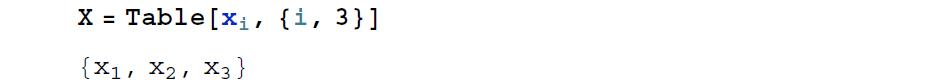
\includegraphics[width=0.9\textwidth]{18.jpg}
\end{figure}
The standard inner product \eqref{eq6} is implemented by a simple dot:
\begin{figure}
  \centering
  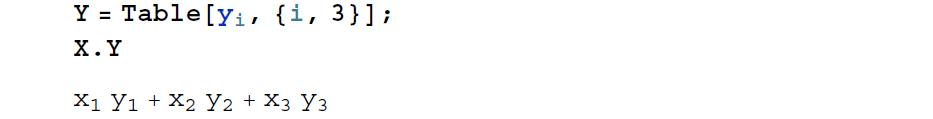
\includegraphics[width=0.9\textwidth]{19.jpg}
\end{figure}
The induced norm \eqref{eq7} is given by the \mathematicafont{\textbf{Norm}}~command:
\begin{figure}
  \centering
  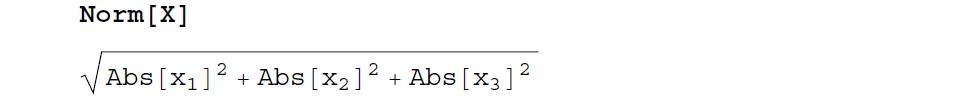
\includegraphics[width=0.9\textwidth]{20.jpg}
\end{figure}
\end{frame}
\begin{frame}[t,allowdisplaybreaks,allowframebreaks]{Orthogonality}
\begin{spacing}{0.9}
\alert{1.3.11. Definition.} Let $(V,\scpp)$ be an inner product vector space.
\begin{enumerate}[1.]
  \item Two vectors $u,v\in V$ are called orthogonal or perpendicular if $\scp{u}{v}=0$. We then write $u\perp v$.
  \item We call
  \begin{equation*}
    M^{\perp}:=\left\{v\in V:\mathop{\forall}_{m\in M}\scp{m}{v}=0\right\}
  \end{equation*}
  the orthogonal complement of a set $M\subset V$.
\end{enumerate}
For short, we sometimes write $v\perp M$ instead of $v\in M^{\perp}$ or $v\perp m$ for all $m\in M$.\\[10pt]
\alert{1.3.12. Lemma.} The orthogonal complement $M^{\perp}$ is a subspace of $V$.\\[10pt]
\alert{Proof.}\\[3pt]
If $v_1,v_2\in M^{\perp}$, then $\scp{v_1+v_2}{m}=\scp{v_1}{m}+\scp{v_2}{m}=0+0=0$ for all $m\in M$, so $v_1+v_2\in M^{\perp}$. Similarly, if $v\in M^{\perp}$ and $\lambda\in\F$, then $\scp{\lambda v}{m}=\overline{\lambda}\scp{v}{m}=0$, so $\lambda v\in M^{\perp}$. Thus $M^{\perp}$ is a subspace of $V$.\qquad\quad$\square$
\newpage
\alert{1.3.13. Pythagoras's Theorem.} Let $(V,\scpp)$ be an inner product space and $M$ some subset of $V$. Let $z=x+y$, where $x\in M$ and $y\in M^{\perp}$. Then
\[\|z\|^2=\|x\|^2+\|y\|^2.\]
\alert{Proof.}\\
We see directly that
\begin{align*}
  \|z\|^2 &=\scp{z}{z}=\scp{x+y}{x+y} \\
   &=\scp{x}{x}+\underbrace{\scp{x}{y}}_{=0}+\underbrace{\scp{y}{x}}_{=0}+\scp{y}{y}  \\
   &=\|x\|^2+\|y\|^2.
\end{align*}
\begin{flushright}
  $\square$
\end{flushright}
\end{spacing}
\end{frame}
\begin{frame}[t,allowdisplaybreaks,allowframebreaks]{Orthonormal Systems}
\begin{spacing}{1}
\alert{1.3.14. Definition.} Let $(V,\scpp)$ be an inner product vector space. A tuple of vectors (\myseries{v}{r})$\in V$ is called a \emph{(finite) orthonormal system} if
\begin{equation*}
  \scp{v_j}{v_k}=\delta_{jk}:=\left\{\begin{aligned}&1\;\;\;\text{for }j=k,\\&0\;\;\;\text{for}~j\neq k,\end{aligned}\right.,\qquad\qquad j,k=1,\ldots,r,
\end{equation*}
i.e., if $\|v_k\|=1$ and $v_j\perp v_k$ for $j\neq k$.\\[12pt]
\alert{1.3.15. Example.} The standard basis vectors in $\R^3$,
\[e_1=\begin{pmatrix}
        1 \\
        0 \\
        0
      \end{pmatrix},\qquad\qquad e_2=\begin{pmatrix}
            0 \\
            1 \\
            0
          \end{pmatrix},\qquad\qquad e_3=\begin{pmatrix}
                0 \\
                0 \\
                1
              \end{pmatrix},\]
form an orthonormal system $(e_1,e_2,e_3)$ with respect to the standard scalar product.
\newpage
\alert{1.3.16. Lemma.} Let $(V,\scpp)$ be an inner product vector space and $\mathcal{F}=$(\myseries{v}{r})$\subset V$ an orthonormal system. Then the elements of $\mathcal{F}$ are linearly independent.\\[6pt]
\alert{Proof.}\\
We want to prove that for any $\lambda_1,\ldots,\lambda_r\in\F$
\begin{equation}\label{eq8}
  \sum_{i=1}^{r}\lambda_iv_i=0
\end{equation}
implies $\lambda_1=\cdots=\lambda_r=0$. We take the scalar product of \eqref{eq8} with $v_1$:
\begin{align*}
  0 &=\scp{v_1}{0}=\scp{v_1}{\lambda_1v_1+\cdots+\lambda_rv_r}  \\
  &=\lambda_1\underbrace{\scp{v_1}{v_1}}_{=1}+\lambda_2\underbrace{\scp{v_1}{v_2}}_{=0}+\cdots+\lambda_r\underbrace{\scp{v_1}{v_r}}_{=0}=\lambda_1,
\end{align*}
so \eqref{eq8} implies $\lambda_1=0$. Similarly, we obtain $\lambda_2=\cdots=\lambda_r=0$.\multido{}{3}{\qquad}$\square$
\end{spacing}
\end{frame}
\begin{frame}[t,allowdisplaybreaks,allowframebreaks]{Orthonormal Bases}
\begin{spacing}{0.9}
\alert{1.3.17. Definition.} Let $(V,\scpp)$ be a finite-dimensional inner product vector space and $\mathcal{B}=(e_1,\ldots,e_n)$ a basis of $V$. If $\mathcal{B}$ is also an orthonormal system, we say that $\mathcal{B}$ is an \emph{orthonormal basis} (ONB).\\[12pt]
\alert{1.3.18. Theorem.} Let $(V,\scpp)$ be a finite-dimensional inner product vector space and $\mathcal{B}=(e_1,\ldots,e_n)$ an orthonormal basis of $V$. Then every $v\in V$ has the basis representation
\[v=\sum_{j=1}^{n}\scp{e_j}{v}e_j.\]
\alert{1.3.19. Definition.} The numbers $\scp{e_j}{v}$ are called \emph{Fourier coef{}ficients} of $v$ with respect to the basis $\mathcal{B}$. The vector
\[\pi_{e_i}v:=\scp{e_i}{v}e_i\]
is called the \emph{projection of v onto} $e_i$.
\newpage
\alert{Proof of Theorem 1.3.18.}\\
Since $\mathcal{B}$ is a basis, for every $v\in V$ there exists coef{}ficients \myseries{\lambda}{n}$\in\F$ such that
\[v=\sum_{j=1}^{n}\lambda_je_j.\]
Now for any $k=1,\ldots,n,$ we have
\[\scp{e_k}{v}=\sum_{j=1}^{n}\lambda_j\scp{e_k}{e_j}=\sum_{j=1}^{n}\lambda_j\delta_{kj}=\lambda_k,\]
so it follows that
\[v=\sum_{j=1}^{n}\lambda_je_j=\sum_{j=1}^{n}\scp{e_j}{v}e_j.\]
\begin{flushright}
  $\square$
\end{flushright}
\end{spacing}
\newpage
\begin{spacing}{1.05}
The following result, which follows directly from Theorem 1.3.18, generalizes Pythagoras's Theorem 1.3.13:\\
\alert{1.3.20. Parseval's Theorem.} Let $(V,\scpp)$ be a finite-dimensional inner product vector space and $\mathcal{B}=\{e_1,\ldots,e_n\}$ an orthonormal basis of $V$. Then
\begin{equation*}
  \|v\|^2=\sum_{i=1}^{n}|\scp{v}{e_i}|^2
\end{equation*}
for any $v\in V$.\\
We have generalized the concepts of angle and orthogonality to vector spaces and thereby obtained Pythagoras's Theorem and now Parseval's inequality. For understanding the geometry of vector spaces (and thereby extending the "elementary" geometry of $\R^3$, the projection of a vector onto subspaces is of fundamental importance. The following theorem
develops this concept a little further.
\end{spacing}
\end{frame}
\begin{frame}[t,allowdisplaybreaks,allowframebreaks]{The Projection Theorem}
\begin{spacing}{1}
\alert{1.3.21. Projection Theorem.} Let $(V,\scpp)$ be a (possibly infinite-dimensional) inner product vector space and (\myseries{e}{r}), $r\in\N$, be an orthonormal system in $V$. Denote $U:=\text{span}\{e_1,\ldots,e_r\}.$\\
Then for every $v\in V$ there exists a unique representation
\begin{equation*}
  v=u+w\multido{}{3}{\qquad}\text{where}~u\in U~\text{and}~w\in U^{\perp}
\end{equation*}
and $u=\sum\limits_{i=1}^{r}\scp{e_i}{v}e_i,\,w:=v-u.$\\
\alert{1.3.22. Definition.} The vector
\begin{equation*}
  \pi_Uv:=\sum_{i=1}^{r}\scp{e_i}{v}e_i
\end{equation*}
is called the orthogonal projection of $v$ onto $U$. The projection theorem
essentially states that $\pi_Uv$ always exists and is independent of the choice
of the orthonormal system (it depends only on the span $U$ of the system).
\newpage
\alert{1.3.23. Example.} Consider the subspace $U=\{(x_1,x_2,x_3)\in\R^3:x_3=0\}$ of $\R^3$. An orthonormal basis of $U$ is given by $\mathcal{B}=\{e_1,e_2\}$, where
\[e_1=\begin{pmatrix}
        1 \\
        0 \\
        0
      \end{pmatrix},\multido{}{3}{\qquad}e_2=\begin{pmatrix}
                                               0 \\
                                               1 \\
                                               0
                                             \end{pmatrix}.\]
Then the projection of a vector $y=(y_1,y_2,y_3)$ onto $U$ is given by
\begin{align*}
  \pi_Uy &=\scp{e_1}{y}e_1+\scp{e_2}{y}e_2  \\
   &=\scp{\begin{pmatrix}
            1 \\
            0 \\
            0
          \end{pmatrix}}{\begin{pmatrix}
                           y_1 \\
                           y_2 \\
                           y_3
                         \end{pmatrix}}\begin{pmatrix}
                                         1 \\
                                         0 \\
                                         0
                                       \end{pmatrix}+\scp{\begin{pmatrix}
                                                            0 \\
                                                            1 \\
                                                            0
                                                          \end{pmatrix}}{\begin{pmatrix}
                                                                           y_1 \\
                                                                           y_2 \\
                                                                           y_3
                                                                         \end{pmatrix}}\begin{pmatrix}
                                                                                         0 \\
                                                                                         1 \\
                                                                                         0
                                                                                       \end{pmatrix}  \\
   &=y_1\begin{pmatrix}
          1 \\
          0 \\
          0
        \end{pmatrix}+y_2\begin{pmatrix}
                           0 \\
                           1 \\
                           0
                         \end{pmatrix}=\begin{pmatrix}
                                         y_1 \\
                                         y_2 \\
                                         0
                                       \end{pmatrix}
\end{align*}
\newpage
\alert{Proof of the Projection Theorem.}\\[11pt]
We first show the uniqueness of the decomposition: Assume $v=u+w=u'+w'$. Then by Pythagoras's theorem,
\begin{equation*}
  0=\|u-u'+(w-w')\|^2=\|u-u'\|^2+\|w-w'\|^2,
\end{equation*}
so $\|u-u'\|=\|w-w'\|=0$. Thus $u=u'$ and $w=w'$.\\[11pt]
Regarding the existence of such a decomposition, it is clear that
\[u=\sum_{i=1}^{r}\scp{e_i}{v}e_i\]
lies in $U$. We need to show that $w\in U^{\perp}$, i.e., $u\perp v-u$.
\newpage
\alert{Proof of the Projection Theorem (continued).}\\
Note first that
\begin{align*}
  \|u\|^2 &=\scp{u}{u}=\scp{\sum_{i=1}^{r}\scp{e_i}{v}e_i}{\sum_{j=1}^{r}\scp{e_j}{v}e_j}  \\
   &=\sum_{i=1}^{r}\sum_{j=1}^{r}\overline{\scp{e_i}{v}}\scp{e_j}{v}\underbrace{\scp{e_i}{e_j}}_{=\delta_{ij}}=\sum_{i=1}^{r}|\scp{e_i}{v}|^2.
\end{align*}
It then follows that
\begin{align*}
  \scp{v-u}{u} &=\scp{v}{u}-\|u\|^2=\scp{v}{\sum_{i=1}^{r}\scp{e_i}{v}e_i}-\|u\|^2  \\
   &=\sum_{i=1}^{r}\scp{e_i}{v}\overline{\scp{e_i}{v}}-\sum_{i=1}^{r}|\scp{e_i}{v}|^2=0.
\end{align*}
\begin{flushright}
  $\square$
\end{flushright}
\end{spacing}
\end{frame}
\begin{frame}[c,shrink]{Orthogonal Subspaces}
\begin{spacing}{1}
An immediate consequence of the Projection Theorem is as follows:\\[12pt]
\alert{1.3.24. Corollary.} Let $(V,\scpp)$ be a (possibly infinite-dimensional) inner product vector space and let $U\subset V$ be a finite-dimensional subspace. Then
\[V=U\oplus U^{\perp}\]
If $V$ is finite-dimensional, then
\[\dim V=\dim U+\dim U^{\perp}.\]
 \\[14pt]
This follows directly from the Projection Theorem with Lemma 1.2.27 and
Theorem 1.2.28.
\end{spacing}
\end{frame}
\begin{frame}[c,shrink]{Bessel's Inequality}
\begin{spacing}{1}
As a consequence of the Projection Theorem 1.3.21 and Pythagoras's Theorem 1.3.13 we obtain the following important result:\\
\alert{1.3.25. Bessel Inequality.} Let $(V,\scpp)$ be an inner product space and (\myseries{e}{n}) an orthonormal system in $V$. Then, for any $v\in V$ and any $r\leq n$,
\begin{equation}\label{eq9}
  \sum_{k=1}^{r}|\scp{e_k}{v}|^2\leq\|v\|^2.
\end{equation}
\alert{Proof.}\\
By Pythagoras's Theorem 1.3.13 we then have $\|v-u\|^2+\|u\|^2=\|v\|^2$, so
\begin{equation*}
  0\leq\|v-u\|^2=\|v\|^2-\|u\|^2=\|v\|^2-\sum_{i=1}^{r}|\scp{e_i}{v}|^2.
\end{equation*}
\begin{flushright}
  $\square$
\end{flushright}
\end{spacing}
\end{frame}
\begin{frame}[t,allowdisplaybreaks,allowframebreaks]{Best Approximation}
\begin{spacing}{0.9}
Now suppose that we want to approximate an element $v\in V$ using a linear combination of the first $r$ elements of an orthonormal system,
\begin{equation}\label{eq10}
  v\approx\sum_{i=1}^{r}\lambda_ie_i,\multido{}{4}{\qquad}\lambda_1,\ldots,\lambda_r\in\F.
\end{equation}
The question is how to choose the coef{}ficients \myseries{\lambda}{r} to make the approximation "as good as possible". We note that
\begin{equation}\label{eq11}
  \begin{split}
     \|v-\sum_{i=1}^{r}\lambda_ie_i\|^2 &=\|v\|^2+\sum_{i=1}^{r}|\lambda_i|^2-\sum_{i=1}^{r}\lambda_i\scp{v}{e_i}-\sum_{i=1}^{r}\overline{\lambda}_i\scp{e_i}{v} \\
       &=\|v\|^2+\sum_{i=1}^{r}\left|\scp{e_i}{v}-\lambda_i\right|^2-\sum_{i=1}^{r}|\scp{e_i}{v}|^2
  \end{split}
\end{equation}
It is clear that \eqref{eq11} is minimal if $\lambda_i=\scp{e_i}{v}$, i.e., the coef{}ficients in \eqref{eq10} are just the Fourier coef{}ficients.
\end{spacing}
\newpage
\begin{spacing}{1.1}
From \eqref{eq11} we can also see that
\begin{equation}\label{eq12}
  \Big\|v-\sum_{i=1}^{r'}\scp{e_i}{v}e_i\Big\|\leq\Big\|v-\sum_{i=1}^{r}\scp{e_i}{v}e_i\Big\|\qquad\text{for any}~r'\geq r,
\end{equation}
so the approximation can only improve when we add further elements of
the orthonormal system $\mathcal{B}$ to the approximation.\\
Clearly, orthonormal systems and bases are extremely useful. We next discuss how to obtain an orthonormal system from any system of vectors.
\end{spacing}
\end{frame}
\begin{frame}[t,allowdisplaybreaks,allowframebreaks]{Gram-Schmidt Orthonormalization}
\begin{spacing}{0.9}
Assume that we have a system of vectors (perhaps a basis)(\myseries{v}{n}) in an inner product vector space $V$. We wish to construct a new system (\myseries{w}{n}) that is orthonormal. We start with $v_1$ and norm it, defining
\[w_1:=\frac{v_1}{\|v_1\|}\]
Next, we want to obtain from $v_2$ a vector $w_2$ such that $w_1\perp w_2$. By Theorem 1.3.21, $v_2$ has a unique representation as a sum $v_2=x+y$, where $x\in\text{span}\{w_1\}$ and $y\in(\text{span}\{w_1\})^{\perp}$. Now $x=\scp{w_1}{v_2}w_1$, so
\[y=v_2-\scp{w_1}{v_2}w_1\in(\text{span}\{w_1\})^{\perp}.\]
(Of course, $y$ is independent and even orthogonal to $w_1$.) It just remains to norm $y$, and we define
\[w_2:=\frac{v_2-\scp{w_1}{v_2}w_1}{\|v_2-\scp{w_1}{v_2}w_1\|}.\]
\newpage
Now we can write
\[v_3=\scp{w_1}{v_3}w_1+\scp{w_2}{v_3}w_2+y,\]
where $y\in(\text{span}\{w_1,w_2\})^{\perp}$. Thus
\[w_3:=\frac{v_3-\scp{w_2}{v_3}w_2-\scp{w_1}{v_3}w_1}{\|v_3-\scp{w_2}{v_3}w_2-\scp{w_1}{v_3}w_1\|}\]
will be normed and orthogonal to $w_1$ and $w_2$. Proceeding in this way, we set
\begin{align*}
  w_1 &:=\frac{v_1}{\|v_1\|} \\
  w_k &:=\frac{v_k-\sum_{j=1}^{k-1}\scp{w_j}{v_k}w_j}{\|v_k-\sum_{j=1}^{k-1}\scp{w_j}{v_k}w_j\|}\qquad\qquad k=2,\ldots,n,
\end{align*}
and hence obtain an orthonormal system as desired.
\newpage
\alert{1.3.26. Example.} Suppose we are given
\[v_1=\begin{pmatrix}
        1 \\
        0 \\
        1
      \end{pmatrix},\qquad\qquad v_2=\begin{pmatrix}
            1 \\
            1 \\
            1
          \end{pmatrix},\qquad\qquad v_3=\begin{pmatrix}
                1 \\
                2 \\
                0
              \end{pmatrix}.\]
Then $\|v_1\|=\sqrt{2}$ so
\[w_1=\frac{1}{\sqrt{2}}\begin{pmatrix}
                          1 \\
                          0 \\
                          1
                        \end{pmatrix}.\]
Next, we calculate the projection of $v_2$ onto $w_1$ and subtract it from $v_2$:
\[v_2-\scp{w_1}{v_2}w_1=\begin{pmatrix}
                          1 \\
                          1 \\
                          1
                        \end{pmatrix}-\left(\frac{1}{\sqrt{2}}\cdot1+\frac{1}{\sqrt{2}}\cdot1\right)\frac{1}{\sqrt{2}}\begin{pmatrix}
                                                                                                                        1 \\
                                                                                                                        0 \\
                                                                                                                        1
                                                                                                                      \end{pmatrix}=\begin{pmatrix}
                                                                                                                                      0 \\
                                                                                                                                      1 \\
                                                                                                                                      0
                                                                                                                                    \end{pmatrix}\]
\newpage
Since the norm of this vector is already one, we have
\[w_2=\begin{pmatrix}
        0 \\
        1 \\
        0
      \end{pmatrix}.\]
Next, we calculate
\[v_3-\scp{w_2}{v_3}w_2-\scp{w_1}{v_3}w_1=\begin{pmatrix}
                                            1 \\
                                            2 \\
                                            0
                                          \end{pmatrix}-2\begin{pmatrix}
                                                           0 \\
                                                           1 \\
                                                           0
                                                         \end{pmatrix}-\frac{1}{2}\begin{pmatrix}
                                                                                    1 \\
                                                                                    0 \\
                                                                                    1
                                                                                  \end{pmatrix}=\frac{1}{2}\begin{pmatrix}
                                                                                                             1 \\
                                                                                                             0 \\
                                                                                                             -1
                                                                                                           \end{pmatrix}\]
Norming,
\[w_3=\frac{1}{\sqrt{2}}\begin{pmatrix}
                          1 \\
                          0 \\
                          -1
                        \end{pmatrix}.\]
\end{spacing}
\end{frame}
\begin{frame}[c,allowdisplaybreaks,allowframebreaks]{Projections and Gram-Schmidt}
\begin{spacing}{1}
\includegraphics[scale=0.05]{mathematica.jpg}~~We can use the \mathematicafont{\textbf{Normalize}}~command to create a normed vector:\\[11pt]
~~~~~~\mathematicafont{$\text{\textcolor[rgb]{0.00,0.00,1.00}{\textbf{v}}}_\text{\textbf{1}}$\:\textbf{=}\:\textbf{\{1,0,1\}};}\\
~~~~~~\mathematicafont{$\text{\textcolor[rgb]{0.00,0.00,1.00}{\textbf{w}}}_\text{\textbf{1}}$\:\textbf{=}\;\textbf{Normalize[}$\text{\textcolor[rgb]{0.00,0.00,1.00}{\textbf{v}}}_\text{\textbf{1}}$\textbf{]}}\\[9pt]
~~~~~~\mathematicafont{\{$\frac{\text{1}}{\sqrt{\text{2}}}$,0,$\frac{\text{1}}{\sqrt{\text{2}}}$\}}\\[10pt]
The projection of $v_2$ onto $w_1$ can be calculated through the \mathematicafont{\textbf{Projection}}\\command.\\[10pt]
~~~~~~\mathematicafont{$\text{\textcolor[rgb]{0.00,0.00,1.00}{\textbf{v}}}_\text{\textbf{2}}$\:\textbf{=}\:\textbf{\{1,1,1\}};}\\
~~~~~~\mathematicafont{\textbf{$\text{\textcolor[rgb]{0.00,0.00,1.00}{\textbf{w}}}_\text{\textbf{2}}$\:\textbf{=}\;$\dfrac{\text{\textcolor[rgb]{0.00,0.00,1.00}{v}}_\text{2}-\text{Projection[}\text{\textcolor[rgb]{0.00,0.00,1.00}{v}}_\text{2},\text{\textcolor[rgb]{0.00,0.00,1.00}{w}}_\text{1}\text{]}}{\text{Norm[\textcolor[rgb]{0.00,0.00,1.00}{v}}_\text{2}-\text{Projection[\textcolor[rgb]{0.00,0.00,1.00}{v}}_\text{2,}\text{\textcolor[rgb]{0.00,0.00,1.00}{w}}_\text{1}\text{]]}}$}}\\[10pt]
~~~~~~\mathematicafont{\{0,1,0\}}\\[10pt]
Note that addition of vectors and multiplication with numbers work naturally.
\newpage
Mathematica has a built-in command for the Gram-Schmidt procedure, \mathematicafont{\textbf{Orthogonalize}}:\\[10pt]
~~~~~~\mathematicafont{$\text{\textcolor[rgb]{0.00,0.00,1.00}{\textbf{v}}}_\text{\textbf{3}}$\:\textbf{=}\:\textbf{\{1,2,0\}};}\\
~~~~~~\mathematicafont{\textbf{Orthogonalize[\{}\textbf{$\text{\textcolor[rgb]{0.00,0.00,1.00}{v}}_\text{1}$,$\text{\textcolor[rgb]{0.00,0.00,1.00}{v}}_\text{2}$,$\text{\textcolor[rgb]{0.00,0.00,1.00}{v}}_\text{3}$\}]}}\\[12pt]
~~~~~~\mathematicafont{$\left\{\left\{\dfrac{\text{1}}{\sqrt{\text{2}}},0,\dfrac{\text{1}}{\sqrt{\text{2}}}\right\},\{0,1,0\},\left\{\dfrac{\text{1}}{\sqrt{\text{2}}},0,-\dfrac{\text{1}}{\sqrt{\text{2}}}\right\}\right\}$}
\end{spacing}
\end{frame}
\subsection{Linear Maps}
\begin{frame}[c]
\begin{spacing}{2.5}
\tableofcontents[sectionstyle=hide,subsectionstyle=show/shaded/hide] \end{spacing}
\end{frame}
\begin{frame}[t,allowdisplaybreaks,allowframebreaks]{Linear maps on Vector Spaces}
\begin{spacing}{1}
In calculus, physics and engineering applications, a fundamental role is played by functions between vector spaces that are linear:\\[10pt]
\alert{1.4.1. Definition.} Let $(U,\oplus,\odot)$ and $(V,\boxplus,\boxdot)$ be vector spaces that are either both real or both complex. Then a map $L:U\rightarrow V$ is said to be \emph{linear} if it is both \emph{homogeneous}, i.e.,
\[L(\lambda\odot u)=\lambda\boxdot L(u)\eqno{(1.4.1a)}\]
and \emph{additive}, i.e.,
\[L(u\oplus u')=L(u)\boxplus L(u'),\eqno{(1.4.1b)}\]
for all $u,u'\in U$ and $\lambda\in\F$. The set of all linear maps $L:U\rightarrow V$ is denoted by $\mathcal{L}(U,V).$\\[10pt]
\alert{1.4.2. Remark.} A linear map $L:U\rightarrow V$ satisfies $L(0)=0$, where we use the same symbol $0$ for the zero in $U$ or in $V$.
\newpage
\vspace*{14pt}
\alert{1.4.3. Examples.}
\begin{enumerate}[(i)]
\item All linear maps $\R\rightarrow\R$ are of the form $x\mapsto\alpha x$ for some $\alpha\in\R$.
\item For $I\subset\R$, the map $\frac{d}{dx}:f\mapsto f'$ is a linear map $C^1(I)\rightarrow C(I)$.
\item The map $(a_n)\mapsto a_0$ is a linear map from the space of all sequences to $\C$.
\item The map $(a_n)\mapsto \lim_{n\to\infty}a_n$ is linear map from space of all convergent sequences to $\C$.
\item If $\C$ is regarded as a real vector space, the map $z\mapsto\overline{z}$ is linear $\C\rightarrow\C$. It is not linear if $\C$ is regarded as a complex vector space.
\item For any real or complex vector space $V$, the map $V\ni x\mapsto c\in\F$\\ $(\F=\R~\text{or}~\C)$ is linear if and only if $c=0$.
\end{enumerate}
For linear maps, we often write simply $Lu$ instead of $L(u)$.
\end{spacing}
\end{frame}
\begin{frame}[t,shrink]{Linear Maps are Structure-Preserving}
\begin{spacing}{1}
A linear map
\[L:U\to V\]
between vector spaces $(U,\oplus,\odot)$ and $(V,\boxplus,\boxdot)$ is a \emph{structure-preserving map}. What does this mean?\\[10pt]
Suppose (for the moment) that $L:U\to V$ is also bijective. Consider the scalar multiplication of a vector $x\in U$ with a number $\lambda$. There are now two ways of doing this: Either we calculate $\lambda\odot x$ directly, or we use the map $L$ to form $Lx\in V$, then multiply by $\lambda$, then use the inverse map $L^{-1}:V\to U$ to regain an element of U:
\setcounter{equation}{1}
\begin{equation}\label{eq13}
  \begin{diagram}
    \node{U} \arrow{e,t}{L} \arrow{s,l}{\lambda\odot}
    \node{V} \arrow{s,r}{\lambda\boxdot}\\
    \node{U}
    \node{V} \arrow{w,t}{L^{-1}}
  \end{diagram}
\end{equation}
\end{spacing}
\end{frame}
\begin{frame}[t,shrink]{Homomorphisms}
\begin{spacing}{1}
The validity of \eqref{eq13} follows from
\[L^{-1}(\lambda\boxdot Lx)=L^{-1}\left(L(\lambda\odot x)\right)=\lambda\odot x.\]
From now on, we will use $\cdot$ instead of symbols like $\odot$ or $\boxdot$ and $+$ instead of $\oplus$ or $\boxplus$. It is up to the reader (you!) to determine which operation in which space is indicated.\\[10pt]
Since linear maps have this important property of structure preservation,
they deserve an appropriately fancy name: they are also known as (vector
space) \emph{homomorphisms} (the Greek prefix \emph{homo} means "same", while
\emph{morphos} means "shape"). Thus, "homomorphism" and "linear map" both
denote the same thing.\\[10pt]
In fact linear maps are so intertwined with the linear structure of vector
spaces that in the finite-dimensional case it suf{}fices to know how a linear
map acts on basis vectors to determine it completely.
\end{spacing}
\end{frame}
\begin{frame}[t,allowdisplaybreaks,allowframebreaks]{Homomorphisms and Finite-Dimensional Spaces}
\begin{spacing}{1}
\alert{1.4.4. Theorem.} Let $U,V$ be real or complex vector spaces and (\myseries{b}{n}) a basis of $U$ (in particular, it is assumed that $\dim U=n<\infty$). Then for every $n$-tuple (\myseries{v}{n})$\in V^n$ there exists a unique linear map $L:U\to V$ such that $Lb_k=v_k,~k=1,\ldots,n.$\\[8pt]
\alert{Proof.}\\
We first show the uniqueness of $L$: Assume there exists a second homomorphism $M\in\mathcal{L}(U,V)$ with $Mb_k=v_k$. For any $u\in U$ we have numbers \myseries{\lambda}{n} such that $u=\sum\lambda_kb_k$. Then
\begin{equation*}
  \begin{split}
     Lu &=L(\lambda_1b_1+\ldots+\lambda_nb_n)=\sum_{k=1}^{n}\lambda_kL(b_k) \\
     &=\sum_{k=1}^{n}\lambda_kv_k=\sum_{k=1}^{n}\lambda_kM(b_k)=M(\lambda_1b_1+\ldots+\lambda_nb_n)=Mu.
  \end{split}
\end{equation*}
Since this is true for any $u\in U$, we have $L=M$.
\newpage
\alert{Proof (continued).}\\
We now prove the existence of such a linear map. i.e., given the tuple (\myseries{v}{n}) we want to show how to define $L$. We define $L$ by defining it for each $u\in U$. Every $u\in U$ has a unique basis decomposition $u=\sum\lambda_kb_k$ with numbers \myseries{\lambda}{n}$\in\F$. We hence define $Lu$ in the obvious way.
\[Lu:=\sum_{k=1}^{n}\lambda_kv_k.\]
It remains to check that $L$ is linear: if $u,u'\in U$ have coordinates $(\lambda_k)_{k=1}^n$ and $(\lambda_k')_{k=1}^n$, respectively, we have
\[L(u+u')=\sum_{k=1}^{n}(\lambda_k+\lambda_k')v_k=\sum_{k=1}^{n}\lambda_kv_k+\sum_{k=1}^{n}\lambda_k'v_k=Lu+Lu'.\]
The homogeneity of $L$ can be shown similarly.\multido{}{7}{\qquad}$\square$
\end{spacing}
\end{frame}
\begin{frame}[c,shrink]{Coordinate Map}
\begin{spacing}{1.1}
\alert{1.4.5. Remarks.}
\begin{enumerate}[(i)]
  \item The identity map id: $V\to V$, id$(v)=v$, is linear.
  \item The set $\mathcal{L}(U,V)$ is again a vector space when endowed with pointwise addition and scalar multiplication.
  \item If $L_1\in\mathcal{L}(U,V)$ and $L_2\in\mathcal{L}(V,W)$, then $L_2\circ L_1\in\mathcal{L}(U,W)$. (The composition of linear maps is linear.)
\end{enumerate}
\vspace*{10pt}
\alert{1.4.6. Examples.}
\begin{enumerate}[(i)]
  \item If $V$ is a real or complex vector space and (\myseries{b}{n}) a basis of $V$, then the \emph{coordinate map}
      \[\varphi:V\to\F^n,\qquad\qquad v=\sum_{k=1}^{n}\lambda_kb_k\mapsto\begin{pmatrix}
                                           \lambda_1 \\
                                           \vdots\\
                                           \lambda_n
                                         \end{pmatrix}\]
      is linear (and bijective).
\end{enumerate}
\end{spacing}
\end{frame}
\begin{frame}[c,shrink]{Dual Space}
\begin{spacing}{1.1}
\alert{1.4.7. Examples.}
\begin{itemize}
  \item[(ii)] Let $V$ be a real or complex vector space. Then $\mathcal{L}(V,\F)$ is known as the \emph{dual space} of $V$ and denoted by $V^*$. The dual space of $V$ is of course itself a vector space.\\[9pt]
      Let $\dim V=n<\infty$ and $\mathcal{B}=(b_1,\ldots,b_n)$ be a basis of $V$. Then for every $k=1,\ldots,n$ there exists a unique map
      \[b_k^*:V\to\F,\qquad\qquad b_k^*(b_j)=\delta_{jk}=\left\{\begin{aligned}1,\quad &j=k,\\ 0,\quad &j\neq k.\end{aligned}\right.\]
      It turns out (see exercises) that the tuple of maps $B^*=(b_1^*,\ldots,b_n^*)$ is a basis of $V^*=\mathcal{L}(V,\F)$ (called the \emph{dual basis of} $\mathcal{B}$) and thus $\dim V^*=\dim V=n$.
\end{itemize}
\end{spacing}
\end{frame}
\begin{frame}[c,shrink]{Range and Kernel}
\begin{spacing}{1.3}
\alert{1.4.8. Definition.} Let $U,V$ be real or complex vector spaces and $L\in\mathcal{L}(U,V)$. Then we define the range of $L$ by
\[\text{ran}L:=\left\{v\in V:\mathop{\exists}_{u\in U}v=Lu\right\}\]
and the \emph{kernel} of $L$ by
\[\text{ker}L:=\left\{u\in U:~Lu=0\right\}.\]
It is easy to see that $\text{ran}L\subset V$ and $\text{ker}L\subset U$ are subspaces.\\[11pt]
\alert{1.4.9. Remark.} It is not dif{}ficult to see that $L\in\mathcal{L}(U,V)$ is injective if and only if $\text{ker}L=\{0\}$.
\end{spacing}
\end{frame}
\begin{frame}[c]{Nomenclature}
\begin{spacing}{1.1}
According to their properties, there are several fancy names for linear
maps. A homomorphism $L\in\mathcal{L}(U,V)$ is said to be
\begin{itemize}
  \item an isomorphism if $L$ is bijective;
  \item an endomorphism if $U=V$;
  \item an automorphism if $U=V$ and $L$ is bijective;
  \item epimorph if $L$ is surjective;
  \item monomorph if $L$ is injective.
\end{itemize}
\alert{1.4.10. Remark.} If $L$ is an isomorphism, the its inverse, $L^{-1}$ is also linear and hence also an isomorphism.
\end{spacing}
\end{frame}
\begin{frame}[t,allowdisplaybreaks,allowframebreaks]{Isomorphisms}
\begin{spacing}{1.1}
\alert{1.4.11. Theorem.} Let $U,V$ be finite-dimensional vector spaces and $L\in\mathcal{L}(U,V)$. Then $L$ is an isomorphism if and only if for every basis (\myseries{b}{n}) of $U$ the tuple (\myseries{Lb}{n}) is a basis of $V$.\\
\alert{Proof.}\\
\begin{itemize}
  \item[($\Rightarrow$)] Assume that $L$ is bijective. Then for $y\in V$ the pre-image $x=L^{-1}y$ is uniquely determined. Let $x=\sum\lambda_kb_k$ be the representation of $x$ in the basis $\mathcal{B}=(b_1,\ldots,b_n)$. Now
      \[y=L\left(\sum_{k=1}^{n}\lambda_kb_k\right)=\sum_{k=1}^{n}\lambda_k\cdot Lb_k\]
      where the $\lambda_k$ are uniquely determined by $x$, which is uniquely determined by $y$. Thus for any $y$ we can find a representation in terms of (\myseries{Lb}{n}) by considering the pre-image $x=L^{-1}y$.\\
      We still need to show that this representation is unique, i.e., if $y=\sum\mu_k\cdot Lb_k$, then $\mu_k=\lambda_k$. Applying $L^{-1}$, we see that
      \[L^{-1}y=x=\sum_{k=1}^{n}\lambda_kb_k,\qquad
      L^{-1}y=L^{-1}\sum_{k=1}^{n}\mu_k\cdot Lb_k=\sum_{k=1}^{n}\mu_kb_k\]
      and because (\myseries{b}{n}) is a basis we see that $\mu_k=\lambda_k$.
  \item[($\Leftarrow$)] We need to show that $L$ is injective and surjective. Since any $y\in V$ may be written as $y=\sum\lambda_k\cdot Lb_k$, $y$ is obviously the image of $x=\sum\lambda_kb_k\in U$. Thus $L$ is surjective.\\
      To see that $L$ is injective, we show that $\text{ker}L=\{0\}$ (see Remark 1.4.9). Now $Lx=0$ for $x=\sum\lambda_kb_k$ implies $\sum\lambda_k\cdot Lb_k=0$. Since (\myseries{Lb}{n}) is a basis, this means that $\lambda_1=\cdots=\lambda_n=0$, so $x=0$.\multido{}{5}{\qquad}$\square$
\end{itemize}
\newpage
\alert{1.4.12. Definition.} Two vector spaces $U$ and $V$ are called \emph{isomorphic}, written $U\cong V$, if there exists an isomorphism $\varphi:U\to V$.\\[10pt]
\alert{1.4.13. Lemma.} Two finite-dimensional vector spaces $U$ and $V$ are isomorphic if and only if they have the same dimension:
\[U\cong V\qquad\Leftrightarrow\qquad\dim U=\dim V\]
\alert{Proof.}\\
\begin{itemize}
  \item[($\Rightarrow$)] Let $\varphi:U\to V$ be an isomorphism and (\myseries{b}{n}) a basis of $U$ ($\dim U=n$). Then $(\varphi(b_1),\ldots,\varphi(b_n))$ is a basis of $V$ and thus $\dim V=n=\dim U$.
  \item[($\Leftarrow$)] If (\myseries{a}{n}) and (\myseries{b}{n}) are basees of $U$ and $V$, respectively, define an isomorphism $\varphi$ by $\varphi(a_k)=b_k,~k=1,\ldots,n$.
\end{itemize}
\end{spacing}
\end{frame}
\begin{frame}[c,allowdisplaybreaks,allowframebreaks]{The Dimension Formula}
\begin{spacing}{1}
We can now prove a deep and fundamental result on linear maps:\\
\alert{1.4.14. Dimensional Formula.} Let $U,V$ be real or complex vector spaces, $\dim U<\infty$. Let $L\in\mathcal{L}(U,V)$. Then
\begin{equation}\label{eq14}
  \dim\text{ran}L+\dim\text{ker}L=\dim U.
\end{equation}
\alert{Proof.}\\
Let $\dim U=:n<\infty$. Since $\text{ker}L\subset U$, we have $\dim\text{ker}L=:r\leq n$. We choose a basis (\myseries{a}{r}) of the kernel, and use the Basis Completion Theorem 1.2.21 to construct a basis $(a_1,\ldots,a_r,a_{r+1},\ldots,a_n)$ of $U$. Then for any $x=\sum\lambda_ka_k\in U$,
\[Lx=L(\lambda_1a_1+\cdots+\lambda_na_n)=\lambda_{r+1}\underbrace{La_{r+1}}_{=:b_1}+\cdots+\lambda_n\underbrace{La_n}_{=:b_{n-r}}.\]
Thus $\text{ran}L=\text{span}\{b_1,\ldots,b_{n-r}\}$.
\newpage
\alert{Proof.}\\
We now claim that the vectors \myseries{b}{{n-r}} are independent; in that case they form a basis of $\text{ran}L$ and $\dim\text{ran}L=n-r$, proving \eqref{eq14}. Consider the equality
\begin{equation}\label{eq15}
  0=\mu_1b_1+\cdots+\mu_{n-r}b_{n-r}=L(\mu_1a_{r+1}+\cdots+\mu_{n-r}a_n).
\end{equation}
If \eqref{eq15} holds, then $\mu_1a_{r+1}+\cdots+\mu_{n-r}a_n\in\text{ker}L=\text{span}\{a_1,\ldots,a_r\}.$ Thus, there exist \myseries{\lambda}{r} such that
\[\mu_1a_{r+1}+\cdots+\mu_{n-r}a_n-(\lambda_1a_1+\cdots+\lambda_ra_r)=0.\]
Since (\myseries{a}{n}) is a basis of $U$, we thence obtain
\begin{equation}\label{eq16}
  \mu_1=\cdots=\mu_{n-r}=0,\qquad\qquad\lambda_1=\cdots=\lambda_r=0.
\end{equation}
Thus \eqref{eq15} implies \eqref{eq16} and \myseries{b}{{n-r}} are independent.\qquad\qquad\qquad$\square$
\newpage
\alert{1.4.15. Corollary.} Let $U,V$ be real or complex finite-dimensional vector spaces with $\dim U=\dim V$. Then a linear map $L\in\mathcal{L}(U,V)$ is injective if and only if it is surjective.\\[11pt]
\alert{\large{Proof.}}\\[13pt]
\begin{center}
  \begin{equation*}
    \begin{split}
       L~\text{injective}\qquad&\Leftrightarrow \qquad\text{ker}L=\{0\}\\
         &\Leftrightarrow\qquad\dim\text{ker}L=0  \\
         &\Leftrightarrow\qquad\dim\text{ran}L=\dim U=\dim V  \\
         &\Leftrightarrow\qquad\text{ran}L=V  \\
         &\Leftrightarrow\qquad L~\text{surjective}
    \end{split}
  \end{equation*}
\end{center}
\begin{flushright}
  $\square$
\end{flushright}
\end{spacing}
\end{frame}
\subsection{Matrices}
\begin{frame}[c]
\begin{spacing}{2.5}
\tableofcontents[sectionstyle=hide,subsectionstyle=show/shaded/hide] \end{spacing}
\end{frame}
\begin{frame}[c,allowdisplaybreaks,allowframebreaks]{A Calculus of Linear Maps}
\begin{spacing}{0.8}
We have seen in Lemma 1.4.13 that two vector spaces are isomorphic if their dimensions are equal. In particular:
\begin{itemize}
  \item Every real $n$-dimensional vector space is isomorphic to $\R^n$
  \item Every complex $n$-dimensional vector space is isomorphic to $\C^n\cong\R^{2n}$
\end{itemize}
This means that if we can find a \emph{calculus} for linear maps $\R^n\to\R^m$, we can automatically treat maps from an $n$-dimensional space $U$ to an $m$-dimensional space $V$:
\begin{equation*}
  \begin{diagram}
    \node{U} \arrow{e,t}{L} \arrow{s,l}{\varphi_1}
    \node{V} \arrow{s,r}{\varphi_2}\\
    \node{\R^n} \arrow{e,t}{A}
    \node{\R^m}
  \end{diagram}
\end{equation*}
Here $L\in\mathcal{L}(U,V),\varphi_1,\varphi_2$ are isomorphisms and $A\in\mathcal{L}(\R^n,\R^m)$. If
\[L=\varphi_2^{-1}\circ A\circ\varphi_1\]
we obtain all relevant properties of $L$ (range, kernel) by analyzing $A$.
\end{spacing}
\newpage
\begin{spacing}{1.2}
The word \emph{calculus} means a "scheme of calculating" that transforms a
procedure that otherwise needs to be performed individually into an
algorithm that can be (easily) applied in general.\\
For example, the revolutionary aspect of Newton/Leibniz's calculus was
the fact that areas under curves, which earlier had been calculated by hand
for each individual type of curve, could suddenly easily be computed through inverse dif{}ferentiation (by finding the primitive of a function).\\
This was exemplified by the fundamental theorem of calculus. As an
example, compare Exercises 4 and 19 of Chapter 14 of Spivak's book with
the simplicity of applying the Fundamental Theorem of Calculus.\\
In the following, we will establish an analogous calculus for linear maps,
where we are able, due to Lemma 1.4.13, to concentrate on those in $\mathcal{L}(\R^n,\R^m)$.
\end{spacing}
\end{frame}
\begin{frame}[t,shrink]{Matrices}
\begin{spacing}{1}
\alert{1.5.1. Definition.} An $m\times n$ matrix over the matrix over the complex numbers is a map
\[a:\{1,\ldots,m\}\times\{1,\ldots,n\}\to\C,\qquad\qquad(i,j)\mapsto a_{ij}.\]
We represent the graph of $a$ through
\begin{equation*}
  A:=\begin{pmatrix}
       a_{11} & a_{12} & \cdots & a_{1n} \\
       a_{21} & a_{22} & \cdots & a_{2n} \\
       \vdots & \vdots & \ddots & \vdots \\
       a_{m1} & a_{m2} & \cdots & a_{mn}
     \end{pmatrix}=(a_{ij})_{\begin{subarray}~1\leq i\leq m\\ 1\leq j\leq n\end{subarray}}.
\end{equation*}
We denote the set of all $m\times n$ matrices over $\C$ by Mat$(m\times n;\C)$.\\
\alert{1.5.2. Remarks.}
\begin{enumerate}[1.]
  \item With the usual pointwise addition and scalar multiplication of maps, Mat$(m\times n;\C)$ becomes a complex vector space.
  \item Matrices over $\R$ instead of $\C$ are defined in the same way. Occasionally, we may also replace $\C$ by a real or complex vector space.
\end{enumerate}
\end{spacing}
\end{frame}
\begin{frame}[t,allowdisplaybreaks,allowframebreaks]{Matrices as Linear Maps}
\begin{spacing}{1}
Matrices turn out to be important tools in the analysis of linear maps:
every linear map between finite-dimensional vector spaces may be expressed as a matrix, and every matrix corresponds (in a certain way) to some such linear map. We first restrict ourselves to the case of $\R^n$.\\[12pt]
\alert{1.5.3. Theorem.} Each matrix $A\in\text{Mat}(m\times n;\R)$ uniquely determines a linear map $j(A)\in\mathcal{L}(\R^n,\R^m)$ such that the columns $a_{\cdot k}$ are the images of the standard basis vectors $e_k\in\R^n$; in particular,
\[j:\text{Mat}(m\times n;\R)\to\mathcal{L}(\R^n,\R^m)\]
is an isomorphism, Mat$(m\times n;\R)\cong\mathcal{L}(\R^n,\R^m)$, so every map $L\in\mathcal{L}(\R^n,\R^m)$ corresponds to a matrix $j^{-1}(L)$ whose columns $a_{\cdot k}$ are the images of the standard basis vectors $e_k\in\R^n$.
\newpage
\alert{Proof.}\\
Given a matrix $A$ with columns $a_{\cdot k},k=1,\ldots,n,$ we simply define $j(A)$ by
\[j(A):\R^n\to\R^m,\qquad\qquad e_k\mapsto a_{\cdot k},\qquad\qquad k=1,\ldots,n.\]
Given a map $L\in\mathcal{L}(\R^n,\R^m)$ we define $j^{-1}(L)\in\text{Mat}(m\times n;\R)$ by
\[j^{-1}(L)=(a_{\cdot1},\ldots,a_{\cdot n}),\qquad\qquad a_{\cdot k}=L(e_k),\qquad\qquad k=1,\ldots,n.\]
Obviously, $j^{-1}$ is actually the inverse of $j$; hence $j$ is bijective. It remains to show that $j$ is linear. Let $A=(a_{ik}),~B=(b_{ik})$. Then
\[j(A+B)e_k=(a+b)_{\cdot k}=a_{\cdot k}+b_{\cdot k}=j(A)e_k+j(B)e_k,\]
so $j$ is additive. The homogeneity can be shown analogously.
\begin{flushright}
  $\square$
\end{flushright}
\newpage
We have thus established that every matrix $A=(a_{ik})$ represents a linear map $j(A)$. In particular,
\[j(A)e_k=\begin{pmatrix}
            a_{1k} \\
            \vdots \\
            a_{mk}
          \end{pmatrix}=\sum_{i=1}^{n}a_{ik}e_i,\qquad\qquad\qquad k=1,\ldots,n.\]
We also note that we can represents $x\in\R^n$ as
\[x=\begin{pmatrix}
      x_1 \\
      \vdots \\
      x_n
    \end{pmatrix}=x_1\begin{pmatrix}
                       1 \\
                       0 \\
                       \vdots \\
                       0
                     \end{pmatrix}+\cdots+x_n\begin{pmatrix}
                                               0 \\
                                               \vdots \\
                                               0 \\
                                               1
                                             \end{pmatrix}=\sum_{k=1}^{n}x_ke_k.\]
\newpage
Then $j(A)\in\mathcal{L}(\R^n,\R^m)$ acts on a general $x\in\R^n$ as follows,
\begin{equation*}
  \begin{split}
     j(A)x &=j(A)\left(\sum_{i=1}^{n}x_ke_k\right)=\sum_{k=1}^{n}x_kj(A)e_k  \\
           &=\sum_{k=1}^{n}x_k\begin{pmatrix}
                                a_{1k} \\
                                \vdots \\
                                a_{mk}
                              \end{pmatrix}  \\
           &=\begin{pmatrix}
               x_1a_{11}+\cdots+x_na_{1n} \\
               \vdots \\
               x_1a_{m1}+\cdots+x_na_{mn}
             \end{pmatrix}.
  \end{split}
\end{equation*}
\newpage
From a practical point of view, we start with $A\in\text{Mat}(m\times n;\R)$ and some $x\in\R^n$ and obtain
\[\begin{pmatrix}
               x_1a_{11}+\cdots+x_na_{1n} \\
               \vdots \\
               x_1a_{m1}+\cdots+x_na_{mn}
             \end{pmatrix}\in\R^m.\]
It seems unnecessary to include the map $j:\text{Mat}(n\times m;\R)\to\mathcal{L}(\R^n,\R^m)$ in this. In fact, we might directly\emph{ interpret the matrix $A$ as a linear map without mentioning $j$!}\\[11pt]
The isomorphism $j$ can be simply left out; mathematicians routinely consider sets of objects that are isomorphic as being \emph{actually identical}. In this way, $A$ has a \emph{double meaning}: it is on the one hand a matrix, and on the other hand a linear map. This avoids always mentioning a superfluous isomorphism and greatly simplifies the formulation of statements.
\end{spacing}
\newpage
\begin{spacing}{1.2}
We therefore write $Ax$ instead of $j(A)x$; in particular,
\setcounter{equation}{0}
\begin{equation}\label{eq17}
  Ax=\begin{pmatrix}
       a_{11} & \cdots & a_{1n} \\
       \vdots & \ddots & \vdots \\
       a_{m1} & \cdots & a_{mn}
     \end{pmatrix}\begin{pmatrix}
                    x_1 \\
                    \vdots \\
                    x_n
                  \end{pmatrix}=\begin{pmatrix}
                                  x_1a_{11}+\cdots+x_na_{1n} \\
                                  \vdots \\
                                  x_1a_{m1}+\cdots+x_na_{mn}
                                \end{pmatrix}.
\end{equation}
We can interpret \eqref{eq17} as the action of a matrix $A\in\text{Mat}(m\times n;\R)$ on a vector $x\in\R^n$, yielding a vector $Ax\in\R^m$.\\[12pt]
This is the beginning of our \emph{calculus of linear maps}. We now need to develop this further to deal with (e.g.) compositions and inverses of linear
maps.
\end{spacing}
\end{frame}
\begin{frame}[c]{Compositions}
\begin{spacing}{1.2}
Let $\R^n\xrightarrow[]{j(A)}\R^m\xrightarrow[]{j(B)}\R^l$ be linear maps and consider their composition $j(B)\circ j(A)$. We want to find a matrix $C$ such that $j(B)\circ j(A)=j(C)$. Now:
\begin{equation*}
  \begin{split}
     j(B)\circ j(A)e_k &=j(B)\sum_{s=1}^{n}a_{sk}e_s=\sum_{s=1}^{m}a_{sk}j(B)e_s=\sum_{s=1}^{m}a_{sk}\sum_{t=1}^{l}b_{ts}e_t \\
     &=\sum_{t=1}^{l}\underbrace{\left(\sum_{s=1}^{m}b_{ts}a_{sk}\right)}_{=:c_{tk}}e_t
  \end{split}
\end{equation*}
where $C=(c_{tk})\in\text{Mat}(l\times n;\R)$. We thus introduce $C$ as the \emph{matrix product} of $B$ and $A$.
\end{spacing}
\end{frame}
\begin{frame}[t,allowdisplaybreaks,allowframebreaks]{Matrix Product}
\begin{spacing}{0.8}
\alert{1.5.4. Definition.} Let $A\in\text{Mat}(l\times m;\C)$ and $B\in\text{Mat}(m\times n;\C)$. Then we define the \emph{product of} $A=(a_{ik})$ \emph{and} $B=(b_{kj})$ by
\[AB\in\text{Mat}(l\times n;\C),\qquad\qquad AB:=\left(\sum_{k=1}^{m}a_{ik}b_{kj}\right)_{\begin{subarray}
                                               ~i=1,\ldots,l\\j=1,\ldots,n
                                             \end{subarray}}\]
We have seen that the matrix product satisfies $j(A)\circ j(B)=j(AB)$. Furthermore, the product is \emph{associative}, i.e.,
\begin{equation*}
  \begin{split}
     A(BC) &=j^{-1}\left(j(A)\circ j(BC)\right)=j^{-1}\left(j(A)(\circ(j(B)\circ j(C))\right)  \\
           &=j^{-1}\left((j(A)\circ j(B))\circ j(C)\right)=j^{-1}\left(j(AB)\circ j(C)\right)  \\
           &=(AB)C
  \end{split}
\end{equation*}
If $A,B\in\text{Mat}(n\times n;\C)$ both products $AB$ and $BA$ exist; however
\[AB\neq BA,\] so the matrix product is \emph{not comutative}.
\end{spacing}
\newpage
\begin{spacing}{1.1}
The matrix product is easily memorized through "row-by-column multiplication," as seen in the following examples:\\
\alert{1.5.5. Examples.}
\begin{enumerate}[1.]
  \item $A=\begin{pmatrix}
            1 & 2 \\
            3 & 4
          \end{pmatrix},~B=\begin{pmatrix}
                             5 & 6 & 7 \\
                             1 & 0 & 2
                           \end{pmatrix},$\\
        $AB=\begin{pmatrix}
             1\cdot5+2\cdot1 & 1\cdot6+2\cdot0 & 1\cdot7+2\cdot2 \\
             3\cdot5+4\cdot1 & 3\cdot6+4\cdot0 & 3\cdot7+4\cdot2
           \end{pmatrix}=\begin{pmatrix}
                           7 & 6 & 11 \\
                           19 & 18 & 29
                         \end{pmatrix}$
  \item $A=\begin{pmatrix}
             1 & 1 \\
             2 & 2
           \end{pmatrix},~B=\begin{pmatrix}
                              2 & 1 \\
                              1 & 0
                            \end{pmatrix},~AB=\begin{pmatrix}
                                                3 &1 \\
                                                6 & 2
                                              \end{pmatrix},~BA=\begin{pmatrix}
                                                                  4 &4 \\
                                                                  1 & 1
                                                                \end{pmatrix}$
  \item $A=\begin{pmatrix}
             1 & 0 \\
             0 & 1
           \end{pmatrix},B=\begin{pmatrix}
                             2 & 1 \\
                             1 & 0
                           \end{pmatrix},AB=\begin{pmatrix}
                                              2 &1 \\
                                              1 & 0
                                            \end{pmatrix}=BA$
  \item $A=\begin{pmatrix}
             0 & \alpha \\
             0 & 0
           \end{pmatrix},~A^2=AA=\begin{pmatrix}
                                   0 & 0 \\
                                   0 & 0
                                 \end{pmatrix}\,\,\,\forall\alpha\in\C$
\end{enumerate}
\end{spacing}
\end{frame}
\begin{frame}[t,shrink]{Matrix Transpose}
\begin{spacing}{1}
For $A=(a_{ij})\in\text{Mat}(m\times n;\F)$ we define the \emph{transpose} of $A$ by
\[A^T\in\text{Mat}(n\times m;\F),\qquad\qquad\qquad A^T=(a_{ji}).\]
For example,
\[\begin{pmatrix}
    5 & 6 & 7 \\
    1 & 0 & 2
  \end{pmatrix}^T=\begin{pmatrix}
                    5 & 1 \\
                    6 & 0 \\
                    7 & 2
                  \end{pmatrix}.\]
We also define the \emph{adjoint}
\[A^*\in\text{Mat}(n\times m;\F),\qquad\qquad\qquad A^*=\overline{A}^T=(\overline{a_{ji}}).\]
where in addition to the transpose the complex conjugate of each entry is
taken.\\[9pt]
It is easy to see (in the assignments) that for $A\in\text{Mat}(m\times n;\F),~x\in\F^m,~y\in\F^n$,
\[\scp{x}{Ay}=\scp{A^*x}{y}.\]
\end{spacing}
\end{frame}
\begin{frame}[c]{Matrices}
\begin{spacing}{1}
\includegraphics[scale=0.05]{mathematica.jpg} ~~In Mathematica, a matrix is defined as follows:
\begin{figure}
  \centering
  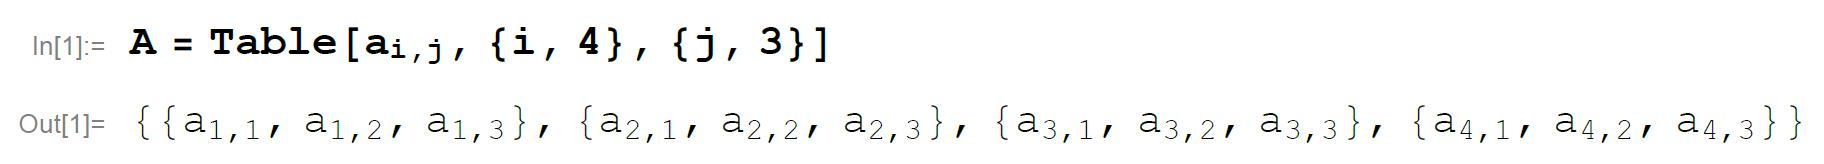
\includegraphics[width=\textwidth]{23.jpg}
\end{figure}
The \mathematicafont{\textbf{MatrixForm}} ~command can be used for nicer formatting.
\begin{figure}
  \centering
  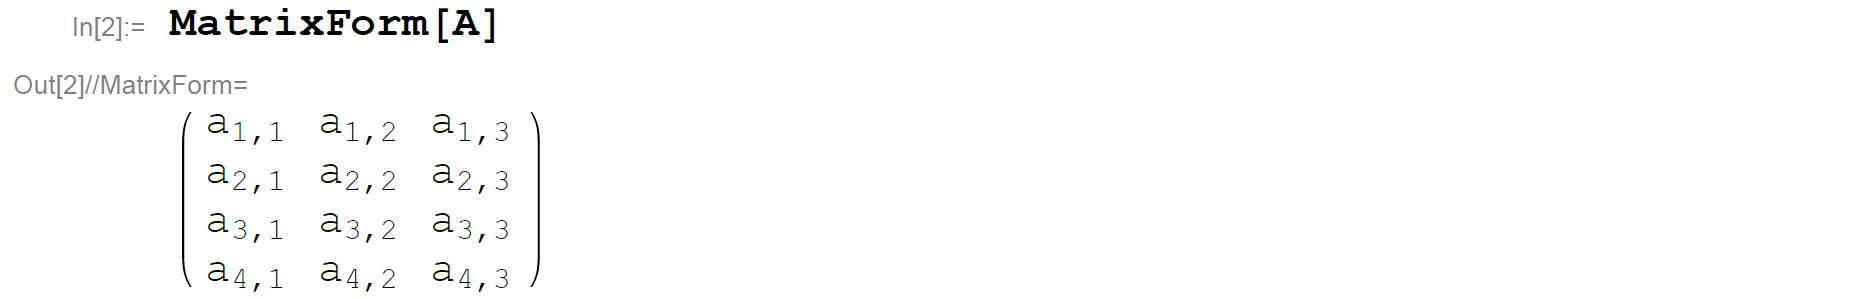
\includegraphics[scale=0.4]{24.jpg}
\end{figure}
\end{spacing}
\end{frame}
\begin{frame}[t]{Matrix Multiplication}
\begin{spacing}{1.2}
\includegraphics[scale=0.05]{mathematica.jpg} ~~Matrix multiplication works using the same dot as for the inner product:
\begin{figure}
  \centering
  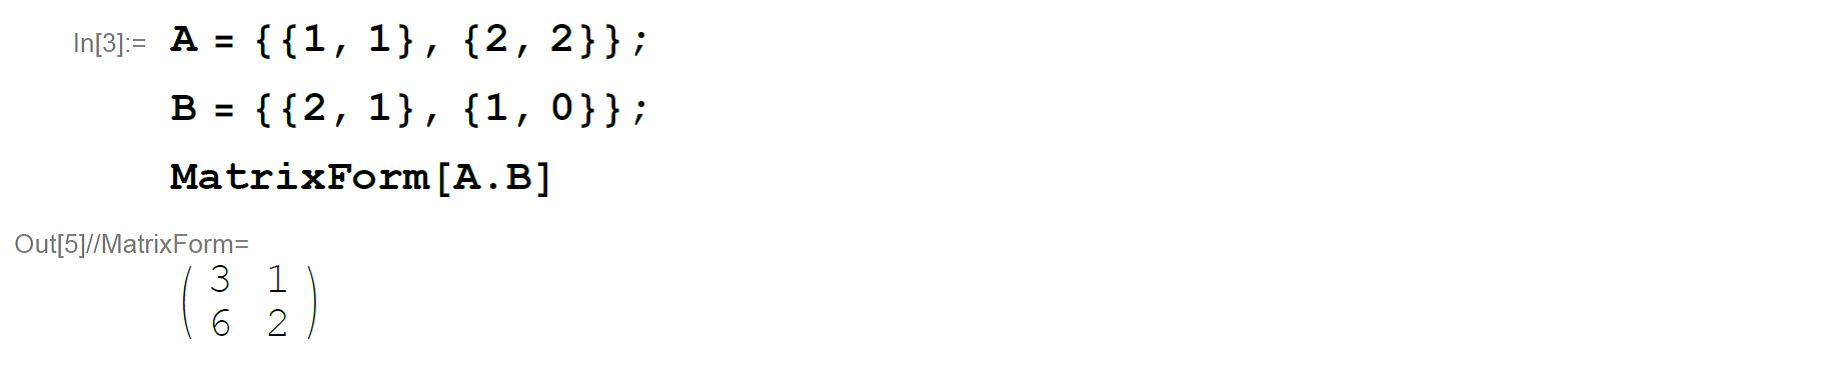
\includegraphics[width=\textwidth]{25.jpg}
\end{figure}
The \mathematicafont{\textbf{Transpose}}~command gives the transpose:
\begin{figure}
  \centering
  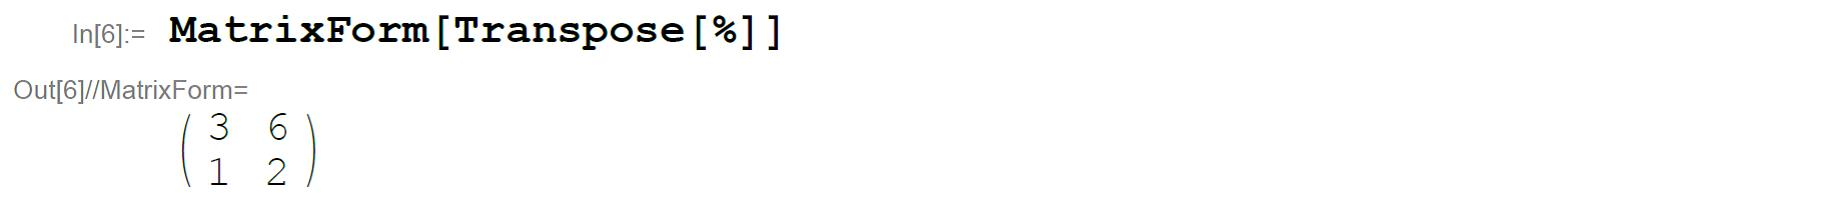
\includegraphics[width=\textwidth]{26.jpg}
\end{figure}
\end{spacing}
\end{frame}
\begin{frame}[t,allowdisplaybreaks,allowframebreaks]{Matrix Multiplication}
\begin{spacing}{1}
There are two very useful facts to keep in mind:
\begin{enumerate}[(i)]
  \item When a vector $x\in\R^n$ is multiplied by a matrix $A\in\text{Mat}(m\times n)$, the result is a linear combination of the column vectors of $A$. For illustration, in the case of $n=3$ and $m=2$, we have
      \begin{equation*}
        \begin{split}
           \begin{pmatrix}
             a_{11} & a_{12} & a_{13} \\
             a_{21} & a_{22} & a_{23}
           \end{pmatrix}\begin{pmatrix}
                          x_1 \\
                          x_2 \\
                          x_3
                        \end{pmatrix} &=\begin{pmatrix}
                            a_{11}x_1+a_{12}x_2+a_{13}x_3 \\
                            a_{21}x_1+a_{22}x_2+a_{23}x_3
                          \end{pmatrix} \\
             &=x_1\binom{a_{11}}{a_{21}}+x_2\binom{a_{12}}{a_{22}}+x_3\binom{a_{13}}{a_{23}}
        \end{split}
      \end{equation*}
  \item When a matrix $B$ is multiplied by a matrix $A$, the result is a matrix
whose columns are the products of the columns of $B$ multiplied with
$A$. Again, for illustration, we give a simple example.
\newpage
Write
\[A=\begin{pmatrix}
      a_{11} & a_{12} \\
      a_{21} & a_{22}
    \end{pmatrix},\qquad\qquad B=\begin{pmatrix}
        b_{11} & b_{12} & b_{13} \\
        b_{21} & b_{22} & b_{23}
      \end{pmatrix}=(b_1,b_2,b_3)\]
where
\[b_1=\binom{b_{11}}{b_{21}},\qquad b_2=\binom{b_{12}}{b_{22}},\qquad
b_3=\binom{b_{13}}{b_{23}}.\]
Then
\begin{equation*}
  \begin{split}
     AB &=\begin{pmatrix}
      a_{11} & a_{12} \\
      a_{21} & a_{22}
    \end{pmatrix}\begin{pmatrix}
        b_{11} & b_{12} & b_{13} \\
        b_{21} & b_{22} & b_{23}
      \end{pmatrix} \\
       &=\begin{pmatrix}
 a_{11} b_{11}+a_{12} b_{21} & a_{11} b_{12}+a_{12} b_{22} & a_{11} b_{13}+a_{12} b_{23} \\
 a_{21} b_{11}+a_{22} b_{21} & a_{21} b_{12}+a_{22} b_{22} & a_{21} b_{13}+a_{22} b_{23} \\
\end{pmatrix} \\
       &=(Ab_1,Ab_2,Ab_3).
  \end{split}
\end{equation*}
\end{enumerate}
\end{spacing}
\end{frame}
\begin{frame}[t,shrink]{Matrix of a Linear Map}
\begin{spacing}{0.9}
We are now able to properly define the matrix of a linear map between two
finite-dimensional vector spaces.\\
Let $U,V$ be finite-dimensional real or complex vector spaces with bases
\[\mathcal{A}=(a_1,\ldots,a_n)\subset U\qquad\qquad\text{and}\qquad\qquad\mathcal{B}=(b_1,\ldots,b_m)\subset V.\]
Define the isomorphisms
\begin{center}
$\varphi_{\mathcal{A}}:U\xrightarrow[]{\cong}\R^n,\qquad\qquad\varphi_{\mathcal{A}}(a_j)=e_j,\qquad\qquad j=1,\ldots,n,$\\
$\varphi_{\mathcal{B}}:V\xrightarrow[]{\cong}\R^m,\qquad\qquad\varphi_{\mathcal{B}}(b_j)=e_j,\qquad\qquad j=1,\ldots,m.$ \end{center}
Then any linear map $L\in\mathcal{L}(U,V)$ induces a matrix $A=\Phi_{\mathcal{A}}^{\mathcal{B}}(L)\in\text{Mat}(m\times n;\R)$ through
\begin{equation*}
  \begin{diagram}
     \node{U} \arrow{e,t}{L} \arrow{s,l}{\varphi_{\mathcal{A}}}
    \node{V} \arrow{s,r}{\varphi_{\mathcal{B}}}\\
    \node{\R^n} \arrow{e,t}{A}
    \node{\R^m}
  \end{diagram}
  \qquad\qquad\Phi_{\mathcal{A}}^{\mathcal{B}}(L)=A=\varphi_{\mathcal{B}}\circ L\circ\varphi_{\mathcal{A}}^{-1}
\end{equation*}
\end{spacing}
\end{frame}
\begin{frame}[t,allowdisplaybreaks,allowframebreaks]{Matrix of Complex Conjugation}
\begin{spacing}{0.9}
\alert{1.5.6. Example.} Consider $\C$ as a real two-dimensional vector space with basis $\mathcal{B}=(1,i)$. The complex conjugation $L:\C\to\C, z\mapsto\overline{z}$ is then a linear map. We want to determine the matrix of this map with respect to the basis $\mathcal{B}$. The isomorphism is
\[\varphi_\mathcal{B}:\C\to\R^2,\qquad\qquad 1\mapsto\binom{1}{0},\qquad\qquad i\mapsto\binom{0}{1}.\]
Thus $\varphi_\mathcal{B}(a+bi)=\binom{a}{b}$. The most convenient way to determine $A=\Phi_\mathcal{B}^\mathcal{B}(L)$ is to calculate
\[\varphi_\mathcal{B}(a+bi)=\binom{a}{b},\qquad
\varphi_\mathcal{B}\left(L(a+bi)\right)=\varphi_\mathcal{B}(a-bi)=\binom{a}{-b}\]
and then find $A\in\text{Mat}(2\times 2;\R)$ such that $A\binom{a}{b}=\binom{a}{-b}$. It is easily seen that
\[A=\Phi_\mathcal{B}^\mathcal{B}(L)=\begin{pmatrix}
                                      1 & 0 \\
                                      0 & -1
                                    \end{pmatrix}.\]
\newpage
\alert{1.5.7. Example.} If we change the basis we used in the previous example,
we get a dif{}ferent matrix. Let us take the basis $\mathcal{A}=(1+i,1-i)$ for $\C$. Then the isomorphism is
\[\varphi_\mathcal{A}:\C\to\R^2,\qquad\qquad 1+i\mapsto\binom{1}{0},\qquad\qquad 1-i\mapsto\binom{0}{1}.\]
Thus
\begin{equation*}
  \begin{split}
     \varphi_\mathcal{A}(a+bi) &=\frac{1}{2}\varphi_\mathcal{A}\left((a+b)(1+i)+(a-b)(1-i)\right) \\
       &=\frac{a+b}{2}\varphi_\mathcal{A}(1+i)+\frac{a-b}{2}\varphi_\mathcal{A}(1-i)=\frac{1}{2}\binom{a+b}{a-b}.
  \end{split}
\end{equation*}
Hence we need to find $A\in\text{Mat}(2\times 2;\R)$ such that $A\binom{a+b}{a-b}=\binom{a-b}{a+b}$, i.e.,
\[A=\Phi_\mathcal{A}^\mathcal{A}(L)=\begin{pmatrix}
                                      0 & 1 \\
                                      1 & 0
                                    \end{pmatrix}.\]
\end{spacing}
\end{frame}
\begin{frame}[t]{Systems of Equations}
\begin{spacing}{1}
Before we proceed, we take a step back to the beginning of the course. Recall that a system of linear equations was given by
\begin{equation}\label{eq18}
  \begin{aligned}
    a_{11}x_1+\cdots+a_{1n}x_n &=b_1 \\
     &~~\vdots  \\
    a_{m1}x_1+\cdots+a_{mn}x_n &=b_m
  \end{aligned}
\end{equation}
We can express \eqref{eq18} using vectors and matrices by writing
\[Ax=b,\]
where
\[A=\begin{pmatrix}
      a_{11} & \cdots & a_{1n} \\
      \vdots & \ddots & \vdots \\
      a_{m1} & \cdots & a_{mn}
    \end{pmatrix},\qquad x=\begin{pmatrix}
                             x_1 \\
                             \vdots \\
                             x_n
                           \end{pmatrix},\qquad b=\begin{pmatrix}
                               b_1 \\
                               \vdots \\
                               b_m
                             \end{pmatrix}.\]
\end{spacing}
\end{frame}
\begin{frame}[t,allowdisplaybreaks,allowframebreaks]{Elementary Matrix Manipulations}
\begin{spacing}{1}
The Gau\ss-Jordan algorithm introduced \emph{elementary row manipulation}, which we now reformulate in the context of matrices:\\[9pt]
\alert{1.5.8. Elementary Matrix Manipulations.} An elementary row manipulation of a matrix is one of the following:
\begin{enumerate}[(i)]
  \item Swapping (interchanging) of two rows,
  \item Multiplication of a row with a non-zero number,
  \item Addition of a multiple of one row to another row.
\end{enumerate}
The additions and multiplications are performed componentwise in each
row.\\[8pt]
If the word "row" is replaced by "column" these operations are termed
elementary column operations.\\[7pt]
The Gau\ss-Jordan algorithm uses only row operations. We seek to find
matrices that implement these row manipulations through multiplication of
$Ax=b$ from the left.
\newpage
For illustration, we consider the case $n=4, m=3$.\\[8pt]
Consider the most trivial operation possible: we do nothing. This would be
represented by multiplying with the unit matrix,
\[\begin{pmatrix}
    1 & 0 & 0 \\
    0 & 1 & 0 \\
    0 & 0 & 1
  \end{pmatrix}\begin{pmatrix}
                 b_1 \\
                 b_2 \\
                 b_3
               \end{pmatrix}=\begin{pmatrix}
                 b_1 \\
                 b_2 \\
                 b_3
               \end{pmatrix}\]
and
\[\begin{pmatrix}
    1 & 0 & 0 \\
    0 & 1 & 0 \\
    0 & 0 & 1
  \end{pmatrix}\begin{pmatrix}
                 a_{11} & a_{12} & a_{13} & a_{14}\\
                 a_{21} & a_{22} & a_{23} & a_{24}\\
                 a_{31} & a_{32} & a_{33} & a_{34}
               \end{pmatrix}=\begin{pmatrix}
                 a_{11} & a_{12} & a_{13} & a_{14}\\
                 a_{21} & a_{22} & a_{23} & a_{24}\\
                 a_{31} & a_{32} & a_{33} & a_{34}
               \end{pmatrix}\]
 \\[7pt]
Note that we do not need to mention $x$ at all in these equations! This is
the true underlying philosophy of the notational scheme used in the
Gau\ss-Jordan algorithm.
\newpage
Now how would we swap the first and second row? We can see that
\[\underbrace{\begin{pmatrix}
    0 & 1 & 0 \\
    1 & 0 & 0 \\
    0 & 0 & 1
  \end{pmatrix}}_{=:S_{12}}\begin{pmatrix}
                 b_1 \\
                 b_2 \\
                 b_3
               \end{pmatrix}=\begin{pmatrix}
                               b_2 \\
                               b_1 \\
                               b_3
                             \end{pmatrix}\]
and\\[7pt]
\[\begin{pmatrix}
    0 & 1 & 0 \\
    1 & 0 & 0 \\
    0 & 0 & 1
  \end{pmatrix}\begin{pmatrix}
                 a_{11} & a_{12} & a_{13} & a_{14}\\
                 a_{21} & a_{22} & a_{23} & a_{24}\\
                 a_{31} & a_{32} & a_{33} & a_{34}
               \end{pmatrix}=\begin{pmatrix}
                 a_{21} & a_{22} & a_{23} & a_{24}\\
                 a_{11} & a_{12} & a_{13} & a_{14}\\
                 a_{31} & a_{32} & a_{33} & a_{34}
               \end{pmatrix}\]
                \\[8pt]
               Note that we have swapped the first and second row of the unit matrix to
obtain $S_{12}$!
\newpage
Furthermore, in order to add 3 times the second row to the third row, we
would use
\[\begin{pmatrix}
    1 & 0 & 0 \\
    0 & 1 & 0 \\
    0 & 3 & 1
  \end{pmatrix}\begin{pmatrix}
                 b_1 \\
                 b_2 \\
                 b_3
               \end{pmatrix}=\begin{pmatrix}
                               b_1 \\
                               b_2 \\
                               b_3+3b_2
                             \end{pmatrix}\]
and
\begin{multline*}
  \begin{pmatrix}
    1 & 0 & 0 \\
    0 & 1 & 0 \\
    0 & 3 & 1
  \end{pmatrix}\begin{pmatrix}
                 a_{11} & a_{12} & a_{13} & a_{14}\\
                 a_{21} & a_{22} & a_{23} & a_{24}\\
                 a_{31} & a_{32} & a_{33} & a_{34}
               \end{pmatrix} \\
  =\begin{pmatrix}
                 a_{11} & a_{12} & a_{13} & a_{14}\\
                 a_{21} & a_{22} & a_{23} & a_{24}\\
                 a_{31}+3a_{21} & a_{32}+3a_{22} & a_{33}+3a_{23} & a_{34}+3a_{24}
               \end{pmatrix}
\end{multline*}
Again we have performed the elementary row operation on the unit matrix to obtain the matrix that implements this operation.
\newpage
In conclusion, we remark that
\begin{enumerate}[(i)]
  \item An elementary row operation on a system of equations may be simply
considered as a multiplication of $Ax = b$ from the left with a suitable
matrix, a so-called elementary matrix.
  \item An elementary matrix is obtained by applying the desired elementary
row operation to the unit matrix. [Why must this be the case?]
  \item If we apply two elementary operations, the product of their respective matrices gives the matrix corresponding to these two operations, in order.
\end{enumerate}
This means that in solving a system $Ax = b$, the sum of all row operations
in forward elimination and backward substitution may be represented by a
single matrix $S\in\text{Mat}(m\times m;\R)$. We thus have
\[SAx=Sb.\]
If $m=n$, the system $Ax=b$ may have a unique solution; in that case, $SA$ is a diagonal matrix of the form (1.1.3), i.e., $SA=\text{id}$.
\end{spacing}
\end{frame}
\begin{frame}[t,allowdisplaybreaks,allowframebreaks]{Inverse of a Matrix}
\begin{spacing}{1}
Let us now return to the question of finding the inverse of a linear map $A:\R^n\to\R^n$ (of course, we must assume that $A$ is an isomorphism, so
$m = n$). Of course, we say that a matrix is invertible if the corresponding
linear map is invertible and the inverse of a matrix is just the matrix of the inverse map. However, it may be useful to clarify this.\\
\alert{1.5.9. Definition.} A matrix $A\in\text{Mat}(n\times n;\R)$ is called \emph{invertible} if there exists some $B\in\text{Mat}(n\times n;\R)$ such that
\begin{equation}\label{eq19}
  AB=BA=\text{id}=\begin{pmatrix}
                    1 &  & 0 \\
                      & \ddots &  \\
                    0 &  & 1
                  \end{pmatrix}.
\end{equation}
We then write $B=A^{-1}$ and say that $A^{-1}$ is the \emph{inverse} of $A$.\\
\alert{1.5.10. Remark.} The inverse is of course unique; if $B$ and $\widetilde{B}$ both satisfy \eqref{eq19} for some $A$, then
\[B=(\widetilde{B}A)B=\widetilde{B}(AB)=\widetilde{B}.\]
\newpage
\alert{1.5.11. Remark.} It is obvious that the matrix S corresponding to a series of
elementary row manipulations will be invertible, because the operations
themselves are invertible. Thus the matrix $S:\R^m\to\R^m$ represents an isomorphism.\\[9pt]
\alert{1.5.12. Remark.} Given a matrix $A\in\text{Mat}(n\times n;\R)$ (identified with a linear map $L\in\mathcal{L}(\R^n,\R^n)$) and a putative inverse matrix $B=A^{-1}\in\text{Mat}(n\times n;\R)$ it is suf{}ficient to verify that\\[5pt]
\[BA=\text{id}.\]
 \\[5pt]
In this case, $B$ corresponds to a linear map $M$ such that $M\circ L$ is the identity map. Thus $\dim\text{ran}M=n$, so $M$ is bijective. Hence $M$ is invertible and $L=M^{-1}$ is bijective. Then $L\circ M=M\circ L=\text{id}$, so we have $AB=BA=\text{id}$.
\newpage
\alert{1.5.13. Lemma.} Let $A\in\mathcal{L}(\R^n,\R^n)$. Then $A$ is \emph{invertible} if and only if there exists an elementary matrix $S$ corresponding to elementary row operations that transform $A$ into the unit matrix $SA = \text{id}$.\\[8pt]
\alert{Proof.}
\begin{itemize}
  \item[($\Rightarrow$)] If $A$ is bijective, for every $y\in\R^n$ there exists a unique solution $x$ to $Ax=y$. Thus there exists a matrix $S$ corresponding to row operations such that
      \[SAx=x=Sy.\]
      For every $x$ there exists a unique $y$ such that $y=Ax$. Thus $SAx=x$ for every $x\in\R^n$, and so $SA=\text{id}$.
  \item[($\Leftarrow$)] By Remark 1.5.12, $SA=AS=\text{id}$, and by Remark 1.5.10, $S=A^{-1}$ so $A$ is invertible.
\end{itemize}
\begin{flushright}
  $\square$
\end{flushright}
\end{spacing}
\end{frame}
\begin{frame}[c,allowdisplaybreaks,allowframebreaks]{Finding the Inverse}
\begin{spacing}{1.1}
Lemma 1.5.13 tells us how to actually find the inverse of a matrix $A$: it is
simply the elementary matrix that transforms $A$ into the unit matrix. If
this transformation is not possible, $A$ is not invertible.\\[7pt]
\alert{1.5.14. Example.} Consider the matrix
\[A=\begin{pmatrix}
      2 & 3 \\
      2 & 1
    \end{pmatrix}.\]
In order to find the inverse, we transform $A$ into the unit matrix through a sequence of elementary row operations $S$, keeping track of the elementary matrix that implements these operations.
\newpage
\begin{equation*}
\begin{array}{c|c}
  SA & S \\
  \begin{pmatrix}
    2 & 3 \\
    2 & 1
  \end{pmatrix} & \begin{gmatrix}[p]
                    1 & 0 \\
                    0 & 1
                    \rowops
                    \mult{0}{:2}
                    \add[\cdot(-2)]{0}{1}
                  \end{gmatrix} \\
  \begin{pmatrix}
    1 & 3/2 \\
    0 & -2
  \end{pmatrix} & \begin{gmatrix}[p]
                    1/2 & 0 \\
                    -1 & 1
                    \rowops
                    \mult{1}{:(-2)}
                    \add[\cdot(-3/2)]{1}{0}
                  \end{gmatrix} \\
  \begin{pmatrix}
    1 & 0 \\
    0 & 1
  \end{pmatrix} & \underbrace{\begin{pmatrix}
                                -1/4 & 3/4 \\
                                1/2 & -1/2
                              \end{pmatrix}}_{A^{-1}}
\end{array}
\end{equation*}
We may immediately check that
\begin{align*}
  A^{-1}A &=\begin{pmatrix}
                                -1/4 & 3/4 \\
                                1/2 & -1/2
                              \end{pmatrix}\begin{pmatrix}
    2 & 3 \\
    2 & 1
  \end{pmatrix}=\begin{pmatrix}
                  1 & 0 \\
                  0 & 1
                \end{pmatrix} \\
  AA^{-1} &=\begin{pmatrix}
    2 & 3 \\
    2 & 1
  \end{pmatrix}\begin{pmatrix}
                                -1/4 & 3/4 \\
                                1/2 & -1/2
                              \end{pmatrix}=\begin{pmatrix}
                  1 & 0 \\
                  0 & 1
                \end{pmatrix}
\end{align*}
\end{spacing}
\end{frame}
\begin{frame}[t]{Matrix Inverse}
\includegraphics[scale=0.05]{mathematica.jpg}~ Mathematica has a command for finding the inverse:
\begin{figure}
  \centering
  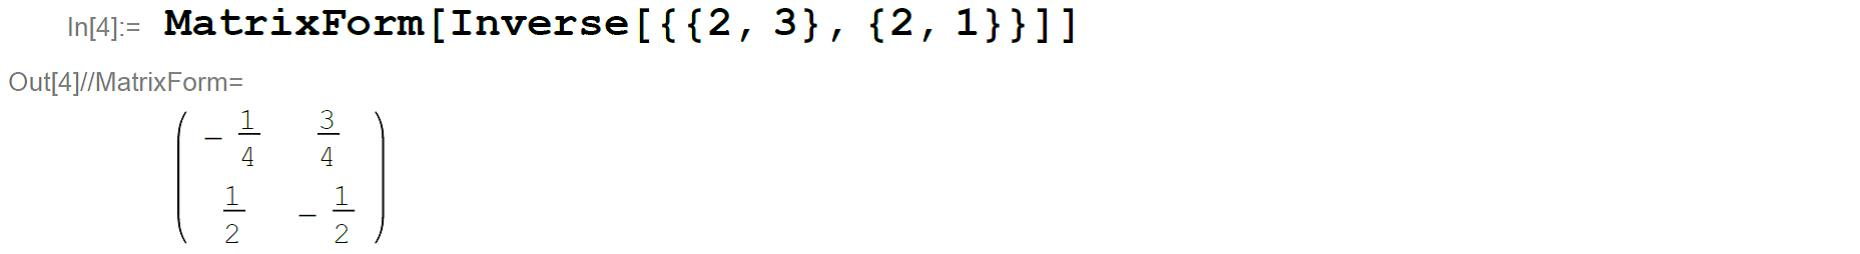
\includegraphics[width=\textwidth]{27.jpg}

\end{figure}
\end{frame}
\begin{frame}[t,allowdisplaybreaks,allowframebreaks]{Inverse Maps}
\begin{spacing}{1.1}
\alert{1.5.15. Remark.} We note that if $A,B\in\text{Mat}(n\times n;\R)$ are invertible, then so is their product $AB\in\text{Mat}(n\times n;\R)$ and $(AB)^{-1}=B^{-1}A^{-1}$.\\
We can use this procedure to find the inverse of any vector space isomorphism $L$:
\begin{equation*}
  \begin{diagram}
    \node{U} \arrow{e,t}{L} \arrow{s,l}{\varphi_\mathcal{A}}
    \node{V} \arrow{s,r}{\varphi_\mathcal{B}}\\
    \node{\R^n} \arrow{e,t}{A}
    \node{\R^m}
  \end{diagram}
  \qquad\qquad L^{-1}=\varphi_\mathcal{A}^{-1}\circ A^{-1}\circ\varphi_\mathcal{B}
\end{equation*}
\alert{1.5.16. Example.} Let $\mathcal{P}_2$ be the space of polynomials of degree not more than 2. Consider the linear map
\[L:\mathcal{P}_2\to\mathcal{P}_2,\qquad ax^2+bx+c\mapsto\frac{a+b+c}{3}x^2+\frac{a+b}{2}x+\frac{a-c}{2}\]
\newpage
We choose a basis (any will do) of $\mathcal{P}_2:\mathcal{B}=(x^2,x,1)$. Then
\[\varphi_\mathcal{B}(ax^2+bx+c)=\begin{pmatrix}
                                   a \\
                                   b \\
                                   c
                                 \end{pmatrix},\qquad \varphi_\mathcal{B}(L(ax^2+bx+c))=\begin{pmatrix}
                                                                     \frac{a+b+c}{3} \\
                                                                     \frac{a+b}{2}\\
                                                                     \frac{a-c}{2}
                                                                   \end{pmatrix}\]
We can read of{}f that
\[A=\begin{pmatrix}
      1/3 & 1/3 & 1/3 \\
      1/2 & 1/2 & 0 \\
      1/2 & 0 & -1/2
    \end{pmatrix}\]
and (with a little bit of work) calculate
\[A^{-1}=\begin{pmatrix}
           3 & -2 & 2 \\
           -3 & 4 & -2 \\
           3 & -2 & 0
         \end{pmatrix}\]
\newpage
Now we are able to calculate the inverse of $L$:
\begin{equation*}
  \begin{split}
     L^{-1}(ax^2+bx+c) &=\varphi_\mathcal{B}^{-1}\circ A^{-1}\circ\varphi_\mathcal{B}(ax^2+bx+c) \\
       &=\varphi_\mathcal{B}^{-1}\circ A^{-1}\begin{pmatrix}
               a \\
               b \\
               c
             \end{pmatrix}  \\
       &=\varphi_\mathcal{B}^{-1}\begin{pmatrix}
           3 & -2 & 2 \\
           -3 & 4 & -2 \\
           3 & -2 & 0
         \end{pmatrix}\begin{pmatrix}
                        a \\
                        b \\
                        c
                      \end{pmatrix}  \\
       &=\varphi_\mathcal{B}^{-1}\begin{pmatrix}
                                   3a-2b+2c \\
                                   -3a+4b-2c \\
                                   3a-2b
                                 \end{pmatrix}  \\
       &=(3a-2b+2c)x^2+(-3a+4b-2c)x+3a-2b
  \end{split}
\end{equation*}
\end{spacing}
\end{frame}
\begin{frame}[c,allowdisplaybreaks,allowframebreaks]{Linear Maps - Active and Passive Points of View}
\begin{spacing}{0.8}
Consider the rotation of the plane $\R^2$ by $45^{\circ}$ in the clockwise direction. In the \textcolor[rgb]{1.00,0.00,0.00}{active} point of view we apply a linear map
\[T:\R^2\to\R^2,\qquad \binom{1}{0}\mapsto\frac{1}{\sqrt{2}}\binom{1}{-1},\qquad \binom{0}{1}\mapsto\frac{1}{\sqrt{2}}\binom{1}{1}\]
so
\[T=\frac{1}{\sqrt{2}}\begin{pmatrix}
                        1 & 1 \\
                        -1 & 1
                      \end{pmatrix}.\]
\begin{figure}
  \centering
  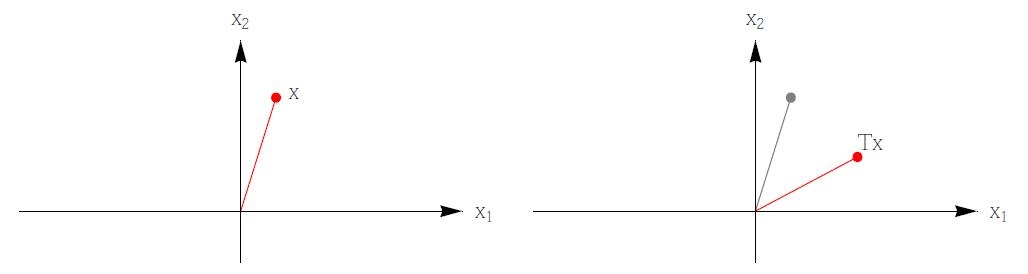
\includegraphics[width=\textwidth]{28.jpg}

\end{figure}
\newpage
In the \textcolor[rgb]{1.00,0.00,0.00}{passive} point of view we do not apply a map $T$ to $x$, but rather transform the coordinate system, i.e., the basis vectors of $\R^2$:
\begin{figure}
  \centering
  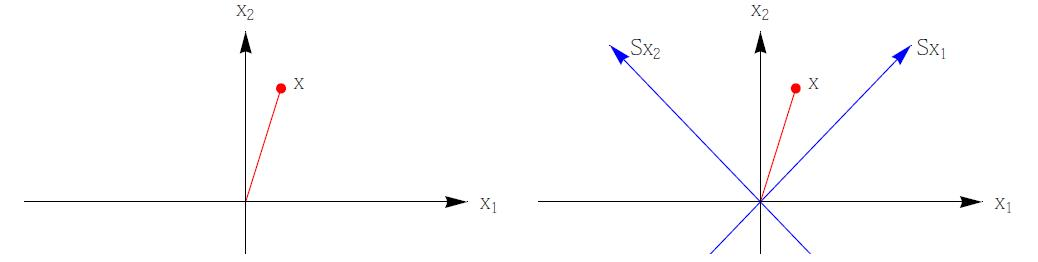
\includegraphics[width=\textwidth,height=2.5cm]{29.jpg}

\end{figure}
The basis vectors must be transformed with the map $S=T^{-1}$. If $e_1=\binom{1}{0}$,\\ $e_2=\binom{0}{1}$ are the original standard basis vectors and $e_1'=T^{-1}e_1,e_2'=T^{-1}e_2$ are the transformed basis vectors, we have
\[x=\sum x_ie_i=\sum x_iTT^{-1}e_i=T\left(\sum x_ie_i'\right).\]
Thus, the point $x$ remains unchanged, but with respect to the new basis $(e_1',e_2')$ it appears that $T$ has been applied.
\end{spacing}
\newpage
\begin{spacing}{1.1}
Both points of view are equally valid; beginners usually prefer to work with
the active point of view (we are \textcolor[rgb]{1.00,0.00,0.00}{doing something}, e.g., rotating the vectors
in the plane), while more experienced mathematicians consider the passive
point of view (we are \textcolor[rgb]{1.00,0.00,0.00}{not doing anything}, just expressing the same vectors in a dif{}ferent basis) more elegant and frequently more useful.
\end{spacing}
\end{frame}
\begin{frame}[c,allowdisplaybreaks,allowframebreaks]{Change of Basis - Active Point of View}
\begin{spacing}{1.05}
A special case that is of particular interest is the changing of a basis. (Of course, any isomorphism can be regarded as a basis change.) Suppose we have a basis $\mathcal{A}=(e_1,\ldots,e_n)$ of $\R^n$ and we wish to represent a vector $x$ not as
\[x=\sum_{i=1}^{n}x_ie_i,\qquad\qquad\qquad x_1,\ldots,x_n\in\R\]
but rather as
\[x=\sum_{i=1}^{n}x_i'e_i',\qquad\qquad\qquad x_1',\ldots,x_n'\in\R\]
where $\mathcal{B}=(e_1',\ldots,e_n')$ is another basis of $\R^n$. Our goal is to calculate the $x_i'$ based on the $x_i$.
\newpage
Assume that there exists some matrix $T$ such that $e_i'=Te_i,~i=1,\ldots,n$. Then
\[T^{-1}x=\sum_{i=1}^{n}x_i'T^{-1}e_i'=\sum_{i=1}^{n}x_i'e_i\]
Thus, if we apply $T^{-1}$ to $x$ we obtain the coordinates $x_i'$ of $x$ with respect to the basis vectors $e_i'=Te_i$. Alternatively, we could say that the change of basis $e_i\mapsto Te_i$ is accomplished by applying $T^{-1}$ to $x$.
\end{spacing}
\end{frame}
\begin{frame}[t,shrink]{Change of Basis - Passive Point of View}
\begin{spacing}{1}
We can also view the passive point of view as follows: we consider the
identity map $\text{id}:\R^2\to\R^2$, but wee imbue the original space $\R^2$ with the standard basis $\mathcal{A}=(e_1,e_2)$, while the image space gets the basis $\mathcal{B}=(e_1',e_2')=(Te_1,Te_2)$. Then we have $\varphi_\mathcal{A}=\text{id}$ and $\varphi_\mathcal{B}=T^{-1}$ consider the matrix $A=\Phi_\mathcal{A}^\mathcal{B}(\text{id})$:
\begin{equation*}
  \begin{diagram}
    \node{\R^2} \arrow{e,t}{\text{id}} \arrow{s,l}{\varphi_\mathcal{A}}
    \node{\R^2} \arrow{s,r}{\varphi_\mathcal{B}}\\
    \node{\R^2} \arrow{e,t}{A}
    \node{\R^2}
  \end{diagram}
  \qquad A\circ\varphi_\mathcal{A}=A=\varphi_\mathcal{B}\circ\text{id}=\varphi_\mathcal{B}=T^{-1}
\end{equation*}
Thus, $T^{-1}$ is just the representing matrix of the basis change.\\[7pt]
Regardless of the point of view, we arrive at a change to a basis $(Te_1,Te_2)$ by applying $T^{-1}$ to $x$. While we have focused on $\R^2$ here, this generalized to $\R^n$ in a natural way.
\end{spacing}
\end{frame}
\begin{frame}[c,allowdisplaybreaks,allowframebreaks]{Reflection in $\R^2$}
\begin{spacing}{1}
\alert{1.5.17. Example.} Consider the reflection of vectors in $\R^2$ by the $x_1$ axis, i.e., the map
\[A:\R^2\to\R^2,\qquad\qquad A\binom{x_1}{x_2}=\binom{x_1}{-x_2}.\]
The matrix representation of $A$ is simply
\begin{equation}\label{eq20}
  A=\begin{pmatrix}
      1 & 0 \\
      0 & -1
    \end{pmatrix}
\end{equation}
Now we want to consider the reflection in $\R^2$ about the line through the vector
\[y=\binom{1}{2}.\]
Of course, the correct matrix for this reflection can be found geometrically.
However, here we want to illustrate how a change of basis can help us
determine this matrix algebraically.
\newpage
Denote by $L$ the reflection about the line through $y=b_1=\binom{1}{2}$. A vector perpendicular to $y$ is $b_2=\binom{-2}{1}$ and so we can choose $\mathcal{A}=(b_1,b_2)$ as a basis. These vectors have the property that
\begin{equation*}
  Lb_1=b_1\qquad\qquad\qquad\text{and}\qquad\qquad\qquad
  Lb_2=-b_2,
\end{equation*}
so in this basis we know how $L$ acts. Now $b_1=Te_1$ and $b_2=Te_2$ where
\begin{equation*}
  T=\begin{pmatrix}
      1 & -2 \\
      2 & 1
    \end{pmatrix}\qquad\text{and we note that}\qquad T^{-1}=\frac{1}{5}\begin{pmatrix}
                        1 & 2 \\
                        -2 & 1
                      \end{pmatrix}.
\end{equation*}
The strategy for calculating the action of the reflection $L$ is now as follows:
\begin{enumerate}[1.]
  \item Change to the basis $(b_1,b_2)$;
  \item Execute the reflection in this basis. It is given by the matrix $A$ of \eqref{eq20};
  \item Change back to the basis $(e_1,e_2)$.
\end{enumerate}
\newpage
Implementing these steps requires applying, in order, $T^{-1}$ to change the basis, $A$ for the reflection in this basis, $T$ to change back:
\[L=TAT^{-1}=\begin{pmatrix}
               1 & -2 \\
               2 & 1
             \end{pmatrix}\begin{pmatrix}
                            1 & 0 \\
                            0 & -1
                          \end{pmatrix}\frac{1}{5}\begin{pmatrix}
                                                    1 &2 \\
                                                    -2 & 1
                                                  \end{pmatrix}=\frac{1}{5}\begin{pmatrix}
                                                                             -3 &4 \\
                                                                             4 & 3
                                                                           \end{pmatrix}\]
It is easily verified that $Lb_1=b_1$ and $Lb_2=-b_2$, as expected.
\end{spacing}
\end{frame}
\subsection{Theory of Systems of Linear Equations}
\begin{frame}[c]
\begin{spacing}{2.5}
\tableofcontents[sectionstyle=hide,subsectionstyle=show/shaded/hide] \end{spacing}
\end{frame}
\begin{frame}[t,shrink]{The Solution Set of Systems of Equations}
\begin{spacing}{1.1}
We briefly return to the theory of solvability of linear systems of equations $Ax=b$. We define the \emph{solution set}
\[\text{Sol}(A,b)=\{x\in\R^n:Ax=b\}.\]
If $x_0\in\R^n$ satisfies
\[Ax_0=b\]
we say that $x_0$ is a \emph{particular solution} of $Ax=b$. The \emph{associated homogeneous solution set} is
\[\text{Sol}(A,0)=\{x\in\R^n:Ax=0\}=\text{ker}A.\]
A very important, fundamental result states:
\begin{quotation}
The solution set of $Ax = b$ is the sum of the homogeneous solution set and a particular solution.
\end{quotation}
\end{spacing}
\end{frame}
\begin{frame}[t,shrink]{Structure of the Solution Set}
\begin{spacing}{1}
\alert{1.6.1. Lemma.} Let $x_0\in\R^n$ be a particular solution of $Ax=b$. Then
\[\text{Sol}(A,b)=\{x_0\}+\text{ker}A=\{y\in\R^n:y=x_0+x,x\in\text{ker}A\}.\]
where the sum of sets is understood as in Definition 1.2.24.\\[7pt]
\alert{Proof.}
\begin{enumerate}[(i)]
  \item $\text{Sol}(A,b)\supset\{x_0\}+\text{ker}A$: Let $x\in\text{ker}A$. Then
      \[A(x_0+x)=Ax_0+Ax=Ax_0=b,\]
      so $x_0+x\in\text{Sol}(a,b).$
  \item $\text{Sol}(A,b)\subset\{x_0\}+\text{ker}A$: Let $v\in\text{Sol}(A,b)$. Then
      \[A(v-x_0)=Av-Ax_0=b-b=0,\]
      so $v-x_0\in\text{ker}A$, implying $v\in\{x_0\}+\text{ker}A$.\multido{}{6}{\qquad}$\square$
\end{enumerate}
\end{spacing}
\end{frame}
\begin{frame}[c,allowdisplaybreaks,allowframebreaks]{Solvabillity of Systems of Equations}
\begin{spacing}{1.1}
The following results follow immediately:\\[7pt]
\alert{1.6.2. Corollary.} If $x_0$ is a solution of $Ax=b$ and \{\myseries{v}{r}\} a basis of $\text{ker}A$, then
\[\text{Sol}(A,b)=\{x\in\R^n:x=x_0+\lambda_1v_1+\cdots+\lambda_rv_r:\lambda_1,\ldots,\lambda_r\in\R\}.\]
Here $r=\dim\text{ker}A$.\\[8pt]
\alert{1.6.3. Corollary.} Suppose that the linear system of equations $Ax=b$ has a solution. Then the solution is unique if and only if $\text{ker}A=\{0\}$.
\newpage
This gives rise to a further, fundamentally important result:\\[7pt]
\alert{1.6.4. Fredholm Alternative.} Let $A$ be an $n\times n$ matrix. Then
\begin{itemize}
  \item \alert{either} $Ax=b$ has a unique solution for any $b\in\R^n$
  \item \alert{or} $Ax=0$ has a non-trivial solution.
\end{itemize}
\vspace*{10pt}
\alert{Proof.}\\
Either $\text{ker}A=\{0\}$ (in which case $Ax=b$ has the solution $x=A^{-1}b$ for any $b\in\R^n$) or $x_0\in\text{ker}A$ is a non-trivial solution of $Ax=0$.\multido{}{5}{\qquad}$\square$ \\[8pt]
The Fredholm alternative occurs in many more complicated contexts. This
is the most basic case.
\end{spacing}
\end{frame}
\begin{frame}[c,allowdisplaybreaks,allowframebreaks]{Matrix Rank}
\begin{spacing}{1}
\alert{1.6.5. Definition.} Let $A\in\text{Mat}(m\times n;\F)$ be a matrix with columns $a_{\cdot j}\in\F^n$,\\$1\leq j\leq n$, and rows $a_{i\cdot}\in\F^n,1\leq i\leq m$. Then we define
\begin{itemize}
  \item the \emph{column rank} of $A$ to be
      \[\text{column rank}A:=\dim\text{span}\{a_{\cdot 1},\ldots,a_{\cdot n}\}\]
  \item and the \emph{row rank} of $A$ to be
      \[\text{row rank}A:=\dim\text{span}\{a_{1\cdot},\ldots,a_{m\cdot}\}.\]
\end{itemize}
\alert{1.6.6. Remark.} From the definition of a matrix it is obvious that the column rank of $A$ equals dim ran $A$.\\[8pt]
The column rank is also the greatest number of independent column
vectors $a_{\cdot j}$ that can be selected from all columns. This is analogously true for the row rank.
\newpage
\alert{1.6.7. Theorem.} Let $A\in\text{Mat}(m\times n;\F)$. Then the column rank is equal to the row rank and we simply write
\[\text{rank}~A:=\text{column rank}~A=\text{row rank}~A.\]
\alert{Long Proof.}\\[7pt]
We first note that the row rank of $A$ does not change if we interchange
rows of $A$ and the same is true for the column rank if we interchange
columns. Write
\[r:=\text{column rank}~A,\qquad\qquad s:=\text{row rank}~A.\]
Then we can assume that the rows $a_{1\cdot},\ldots,a_{s\cdot}$ are linearly independent and the same is true for the columns $a_{\cdot 1},\ldots,a_{\cdot r}$. Furthermore, any column vector $a_{\cdot i}$ is a linear combination of the vectors $\{a_{\cdot 1},\ldots,a_{\cdot r}\}$.
\newpage
\alert{Long Proof (continued).}\\[7pt]
\alert{Step 1: $s\leq r$} Suppose that $s>r$ and that a linear combination of the first $s$ rows vanishes, i.e.,
\setcounter{equation}{0}
\begin{equation}\label{eq21}
  \sum_{i=1}^{s}x_ia_{i\cdot}=0,\qquad\qquad\qquad x_1,\ldots,x_s\in\F.
\end{equation}
Since the rows are independent, this must imply that $x_1=\cdots=x_s=0$.
Now \eqref{eq21} can be written as a system of equations because each column of the row vector on the left-hand side must vanish. In particular, the first $r$ columns must vanish and we obtain the $r$ equations
\begin{equation}\label{eq22}
  \sum_{i=1}^{s}x_ia_{ij}=0,\qquad\qquad\qquad j=1,\ldots,r.
\end{equation}
\newpage
\alert{Long Proof (continued).}\\[7pt]
Under our assumption of $s>r$, by the Fundamental Lemma 1.1.8 there exists a non-zero solution $x=(x_1,\ldots,x_s)$ to the $r$ equations \eqref{eq22}.\\
However, this does not yet imply that there exists a non-zero solution to \eqref{eq21}.\\[6pt]
We now use that every column vector has the representation
\begin{equation}\label{eq23}
  a_{\cdot j}=\sum_{k=1}^{r}\lambda_{jk}a_{\cdot k},\qquad\qquad\qquad j=1,\ldots,n,
\end{equation}
so we have
\begin{equation}\label{eq24}
  a_{ij}=\sum_{k=1}^{r}\lambda_{jk}a_{ik},\qquad
  \lambda_{ij}\in\F,\qquad i=1,\ldots,m,~j=1,\ldots,n.
\end{equation}
\newpage
\alert{Long Proof (continued).}\\[7pt]
Then, for any $j=1,\ldots,n,$
\begin{equation}\label{eq25}
  \sum_{i=1}^{s}x_ia_{ij}=\sum_{i=1}^{s}x_i\sum_{k=1}^{r}\lambda_{jk}a_{ik}=\sum_{k=1}^{r}\lambda_{jk}\underbrace{\sum_{i=1}^{s}x_ia_{ik}}_{=0}=0
\end{equation}
The $n$ equations \eqref{eq25} are equivalent to \eqref{eq21}, so we have a non-zero solution of \eqref{eq21}. Hence, the $s$ rows can not be independent and we arribe at a contradiction.\\[5pt]
\alert{Step 2: $r\leq s.$} By definition, $\text{row rank}A=\text{column rank}A^T$. This implies \[r=\text{column rank}A=\text{row rank}A^T\leq\text{column rank}A^T=\text{row rank}A=s\]
and hence $r=s$.\multido{}{13}{\qquad}$\square$
\newpage
\alert{Short Proof.}\\
In the assignments it will be shown that
\[\text{ran}A^T=(\text{ker}A)^{\perp}.\]
Then, using Corollary 1.3.24 and the dimension formula \eqref{eq14},
\begin{equation*}
  \begin{split}
     \text{row rank}A &=\text{column rank}A^T=\dim\text{ran}A^T=\dim(\text{ker}A)^{\perp} \\
       &=n-\dim\text{ker}A=\dim\text{ran}A=\text{column rank}A.
  \end{split}
\end{equation*}
\end{spacing}
\end{frame}
\begin{frame}[t]{Existence of Solutions}
The fundamental theorem on the existence of solutions to a linear system of equations is the following:\\
\alert{1.6.8. Theorem.} There exists a solution $x$ for $Ax=b$ if and only if $\text{rank}A=\text{rank}(A\,|\,b)$, where
\[(A\,|\,b)=\begin{pmatrix}
          a_{11} & \cdots & a_{1n} & b_1 \\
          \vdots &   & \vdots & \vdots
           \\
          a_{m1} & \cdots & a_{mn} & b_m
        \end{pmatrix}\in\text{Mat}((n+1)\times m).\]
\end{frame}
\begin{frame}[t]{Solvability of Systems of Equations}
\begin{spacing}{1}
\alert{Proof.}\\
We write $A=(a_1,\ldots,a_n)$, where the $a_k\in\R^m$ are column vectors of $A$. Then we use that the range of a matrix is the span of its column vectors and the rank is the dimension of the range, so
\begin{equation*}
  \begin{split}
       &~~~~~Ax=b~\text{has solution} ~x\in\R^n \\
       &\Leftrightarrow b\in\text{ran}A  \\
       &\Leftrightarrow b\in\text{span}(a_1,\ldots,a_n)  \\
       &\Leftrightarrow b ~\text{is not independent of}~ a_1,\ldots,a_n  \\
       &\Leftrightarrow \dim\text{span}(a_1,\ldots,a_n)=\dim\text{span}(a_1,\ldots,a_n,b)  \\
       &\Leftrightarrow \dim\text{ran}A=\dim\text{ran}(A\,|\,b)   \\
       &\Leftrightarrow \text{rank}~A=\text{rank}(A\,|\,b)
  \end{split}
\end{equation*}
\begin{flushright}
  $\square$
\end{flushright}
\end{spacing}
\end{frame}
\begin{frame}[c,allowdisplaybreaks,allowframebreaks]{Manipulating Matrices}
\begin{spacing}{1.1}
\includegraphics[scale=0.05]{mathematica.jpg}~ A matrix is just a list of lists. The command \mathematicafont{\textbf{Append}}~is used to add elements to a list:
\begin{figure}
  \centering
  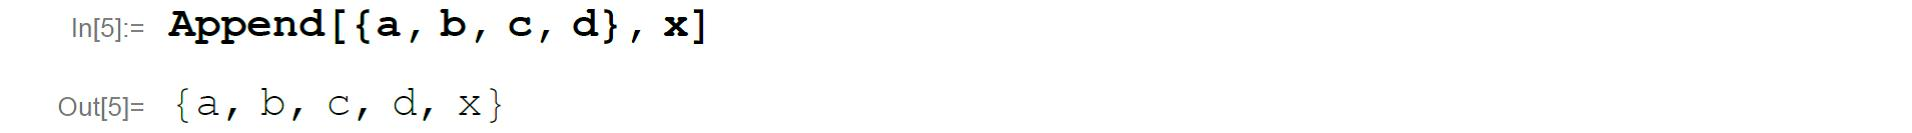
\includegraphics[width=\textwidth]{30.jpg}

\end{figure}
We want to use this to check $\text{rank}A=\text{rank}(A\,|\,b)$. Define a matrix $A$ and a vector $b$ as follows:
\begin{figure}
  \centering
  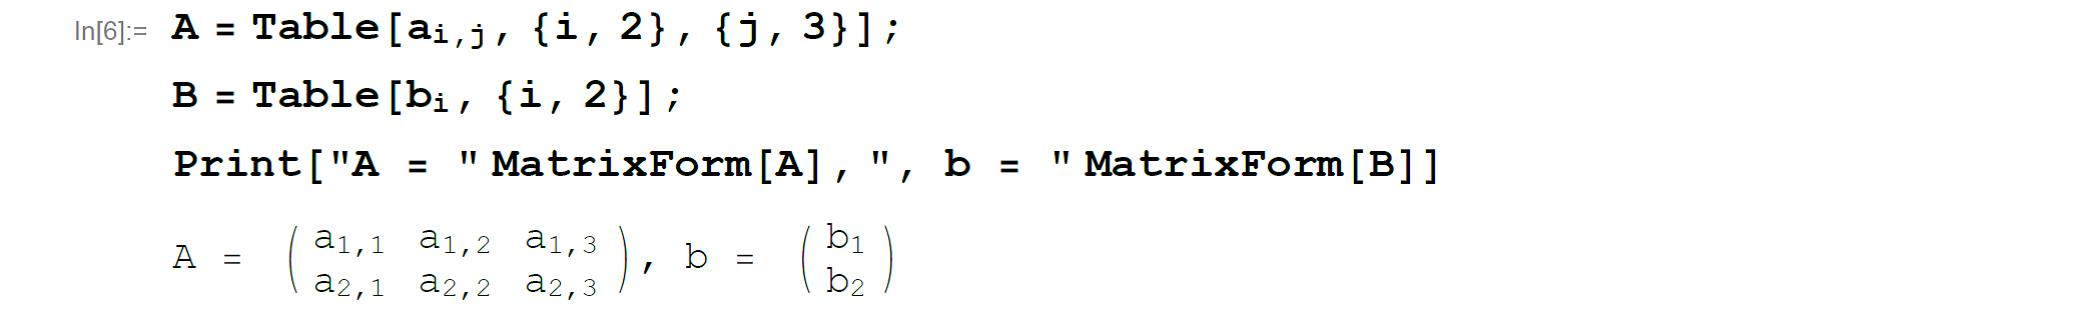
\includegraphics[width=\textwidth]{31.jpg}

\end{figure}
\newpage
Since a matrix is a list of row vectors, it is easy to add a row:
\begin{figure}
  \centering
  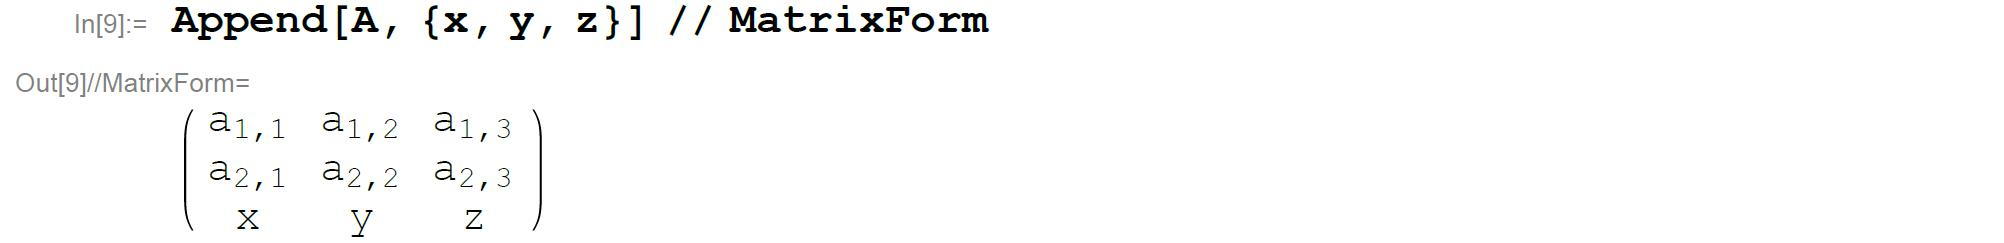
\includegraphics[width=\textwidth]{32.jpg}

\end{figure}
To add a column, we could transpose, add a row, and transpose again:
\begin{figure}
  \centering
  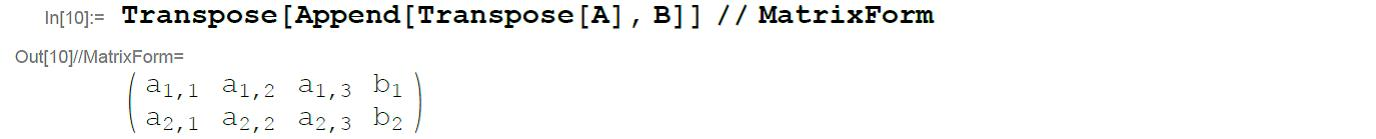
\includegraphics[width=\textwidth]{33.jpg}

\end{figure}
However, the repeated transposition is inef{}ficient and may cost significant computing resources for large matrices.
\newpage
There exists a specialized command to achieve the same result without
transposition:
\begin{figure}
  \centering
  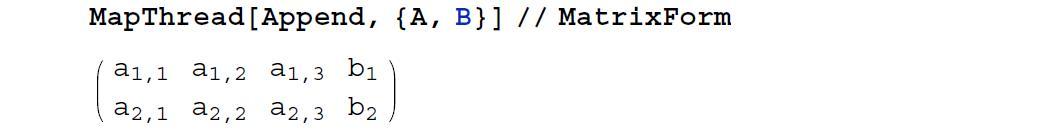
\includegraphics[width=\textwidth]{34.jpg}

\end{figure}
The rank of a matrix is found through the \mathematicafont{\textbf{MatrixRank}}~command.
\newpage
\alert{1.6.9. Example.}
\begin{figure}
  \centering
  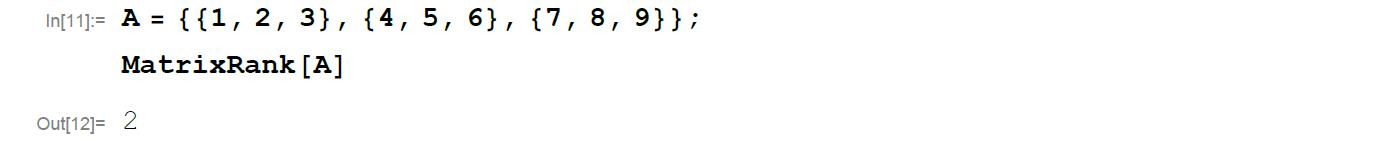
\includegraphics[width=\textwidth]{35.jpg}
\end{figure}
\begin{figure}
  \centering
  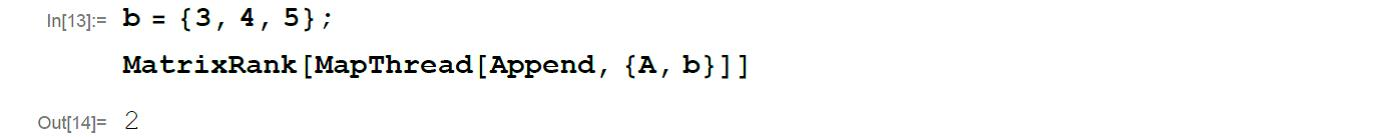
\includegraphics[width=\textwidth]{36.jpg}

\end{figure}
\begin{figure}
  \centering
  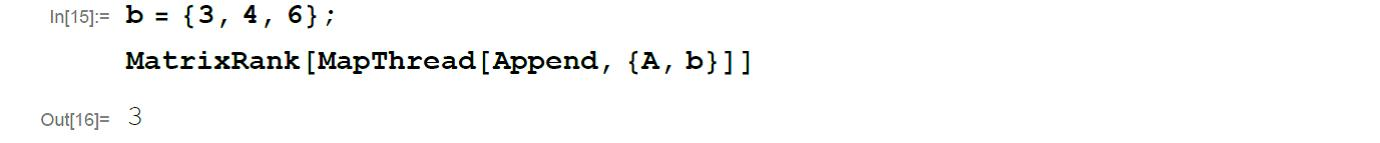
\includegraphics[width=\textwidth]{37.jpg}

\end{figure}
\newpage
The kernel of a matrix is obtained from the \mathematicafont{\textbf{NullSpace}}~command:
\begin{figure}
  \centering
  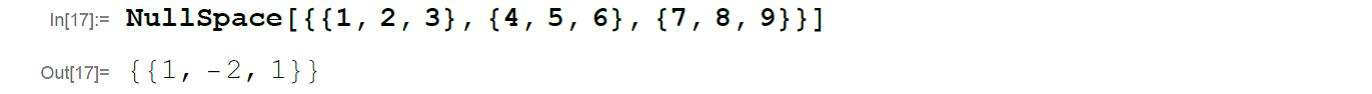
\includegraphics[width=\textwidth]{38.jpg}

\end{figure}
The output is a list of basis vectors of the kernel of the matrix.
\end{spacing}
\end{frame}
\subsection{Determinants}
\begin{frame}[c]
\begin{spacing}{2.5}
\tableofcontents[sectionstyle=hide,subsectionstyle=show/shaded/hide] \end{spacing}
\end{frame}
\begin{frame}[t,shrink]{Parallelograms}
\begin{spacing}{1.1}
We will motivate determinants geometrically (as areas of
parallelograms/volumes of parallelepipeds) rather than algebraically (via
solutions of systems of linear equations).\\[6pt]
Consider a parallelogram $P(a,b)$ spanned by two non-colinear vectors $a,b\in\R^2$.
\begin{columns}[onlytextwidth]
\begin{column}{0.35\textwidth}
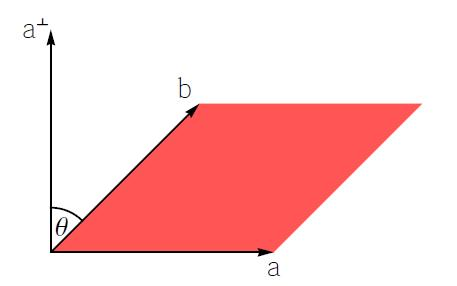
\includegraphics[width=\columnwidth]{para.jpg}
\end{column}
\begin{column}{0.65\textwidth}
We are interested in the area $A(a,b)$ of the parallelogram, which is equal to the area of the rectangle with width $|a|$ and height given by $|b||\cos\theta|$. Let $a=(a_1,a_2),a^{\perp}=(-a_2,a_1)$. Then $a\perp a^{\perp}$, i.e., $\scp{a}{a^{\perp}}=0$ and $|a^{\perp}|=|a|$.
\end{column}
\end{columns}
\vspace*{5pt}
From \eqref{eq7} it follows that
\[|b|\cos\theta=\scp{\frac{a^{\perp}}{|a^{\perp}|}}{b}\]
\end{spacing}
\end{frame}
\begin{frame}[t,shrink]{The Determinant in $\R^2$}
\begin{spacing}{1.05}
We obtain
\[A(a,b)=|a|\left|\scp{\frac{a^{\perp}}{|a^{\perp}|}}{b}\right|=\frac{|a|}{|a^{\perp}|}|\scp{a^{\perp}}{b}|=|\scp{a^{\perp}}{b}|=|a_1b_2-a_2b_1|.\]
We remark that
\[A(a,b)=|\scp{a^{\perp}}{b}|=|a||b|\sin\sphericalangle(a,b)\]
We define the determinant as a map
\setcounter{equation}{0}
\begin{equation}\label{eq26}
  \det:\R^2\times\R^2\to\R,\qquad\det\left(\binom{a_1}{a_2},\binom{b_1}{b_2}\right)=a_1b_2-a_2b_1,
\end{equation}
so that $A(a,b)=|\det(a,b)|$. The determinant is an \emph{oriented area}.\\
Equivalently, the determinant may be regarded as a map
\begin{equation}\label{eq27}
  \det:\text{Mat}(2\times 2;\R)\to\R,\qquad\det\begin{pmatrix}
                         a_1 & b_1 \\
                         a_2 & b_2
                       \end{pmatrix}=a_1b_2-a_2b_1.
\end{equation}
\end{spacing}
\end{frame}
\begin{frame}[c,allowdisplaybreaks,allowframebreaks]{Properties of the Determinant}
\begin{spacing}{1.3}
Both interpretations of the determinant will be used frequently.\\
\alert{1.7.1. Remark.} We note the following properties of the determinant:
\begin{itemize}
  \item[1.] det is \emph{normed}, i.e.,
        \[\det(e_1,e_2)=\det\begin{pmatrix}
                              1 & 0 \\
                              0 & 1
                            \end{pmatrix}=1.\]
  \item[2.] det is \emph{bilinear}:
        \begin{center}
          $\det(\lambda a,b)=\lambda\det(a,b)=\det(a,\lambda b)$,\\
          $\det(a+b,c)=\det(a,c)+\det(b,c)$,\\
          $\det(a,b+c)=\det(a,b)+\det(a,c)$.
        \end{center}
        This can be easily seen geometrically by considering the volumes of
        the parallelograms.
        \newpage
  \item[3.] det is \emph{alternating}, i.e., $\det(a,a)=a_1a_2-a_2a_1=0$. Note that this implies that $\det(a,b)=-\det(b,a)$, since (using the bilinearity)
      \begin{equation*}
        \begin{split}
           0 &=\det(a+b,b+a)  \\
             &=\det(a,a)+\det(b,b)+\det(a,b)+\det(b,a)  \\
             &=\det(a,b)+\det(b,a).
        \end{split}
      \end{equation*}
      (In the case of two variables, an alternating map is often called
      \emph{antisymmetric}.)
\end{itemize}
\end{spacing}
\end{frame}
\begin{frame}[t,shrink]{Vector Product in $\R^3$}
\begin{spacing}{1.2}
We now introduce the "vector product" $a\times b$ of two vectors $a,b\in\R^3$. The vector $a\times b\in\R^3$ is determined by
\begin{itemize}
  \item[1.] its length: we set $|a\times b|=A(a,b)$, the area of the parallelogram spanned by $a$ and $b$ (if $a$ and $b$ are linearly dependent, we set $a\times b=0$);
  \item[2.] its direction: we want $a\times b$ to be orthogonal to $a$ and $b$ - in other words, $a\times b\perp\text{span}\{a,b\}$;
  \item[3.] its orientation: $(a,b,a\times b)$ should form a "right-hand system"
      (defined using the thumb, index finger and middle finger of the right
      hand).
\end{itemize}
This is suf{}ficient to define a unique vector $a\times b$ for $a,b\in\R^3$, i.e., we have a map $\times:\R^3\times\R^3\to\R^3$.\\
\alert{1.7.2. Remark.} In contradistinction to the scalar product, which can be defined on
$\R^n$ for $n=1,2,\ldots,$ the vector product is only defined on $\R^3$.
\end{spacing}
\end{frame}
\begin{frame}{The Right Hand Rule}
\begin{figure}
  \centering
  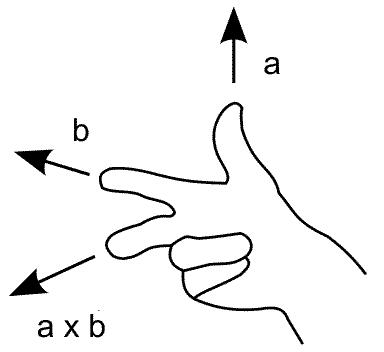
\includegraphics[scale=0.8]{righthand.jpg}

\end{figure}
\begin{center}
  {\tiny\href{https://commons.wikimedia.org/wiki/File:RHR.svg}{Rechte Hand Regel [modified]. Wikimedia Commons. Wikimedia Foundation. Web. 9 May 2012}}
\end{center}
\end{frame}
\begin{frame}[t,shrink]{Properties of the Vector Product in $\R^3$}
\begin{spacing}{1}
Note that the vector product is
\begin{itemize}
  \item[1.] \emph{bilinear}: the homogeneity $(\lambda a)\times b=\lambda(a\times b)=a\times(\lambda b)$ follows from the definition of the cross product, the additivity $a\times(b+c)=a\times b+a\times c,(a+b)\times c=a\times c+b\times c$ is easy to see geometrically when $a, b, c$ are coplanar and slightly more dif{}ficult
      to show when they are not.
  \item[2.] \emph{antisymmetric}: $a\times a=0$, or $a\times b=-b\times a$.
\end{itemize}
We can compute the vector product of the standard basis vectors with
each other:\\[5pt]
\begin{columns}[c,totalwidth=0.9\textwidth]
\begin{column}{0.4\textwidth}
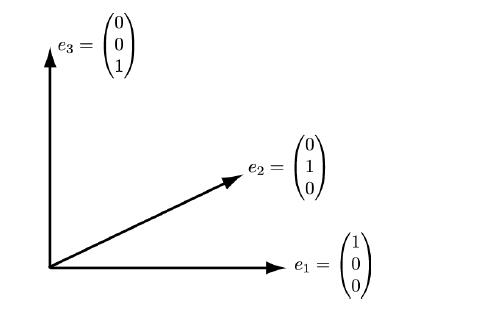
\includegraphics[width=\columnwidth]{84.jpg}
\end{column}
\begin{column}{0.5\textwidth}
\begin{align}\label{1.7.3}
  e_1\times e_2 &=e_3=-e_2\times e_1\nonumber \\
  e_2\times e_3 &=e_1=-e_3\times e_2\nonumber \\
  e_3\times e_1 &=e_2=-e_1\times e_3\nonumber \\
  e_1\times e_1 &=0=e_2\times e_2=e_3\times e_3
\end{align}
\end{column}
\end{columns}
\end{spacing}
\end{frame}
\begin{frame}[t,shrink]{Calculating the Vector Product in $\R^3$}
\begin{spacing}{1.1}
Using the bilinearity and (1.7.3), we can now calculate $a\times b$ for arbitrary $a,b\in\R^3$:
\setcounter{equation}{3}
\begin{equation}\label{1.7.4}
  \begin{split}
     a\times b &=(a_1e_1+a_2e_2+a_3e_3)\times (b_1e_1+b_2e_2+b_3e_3) \\
       &=\sum_{i,j=1}^{3}a_ib_j(e_i\times e_j)  \\
       &=(a_2b_3-a_3b_2)e_1+(a_3b_1-a_1b_3)e_2+(a_1b_2-a_2b_1)e_3  \\
       &=\begin{pmatrix}
           +\det\begin{pmatrix}
                  a_2 & b_2 \\
                  a_3 & b_3
                \end{pmatrix} \\
           -\det\begin{pmatrix}
                  a_1 & b_1 \\
                  a_3 & b_3
                \end{pmatrix} \\
           +\det\begin{pmatrix}
                  a_1 & b_1 \\
                  a_2 & b_2
                \end{pmatrix}
         \end{pmatrix}
  \end{split}
\end{equation}
\end{spacing}
\end{frame}
\begin{frame}[t,shrink]{Parallel Epipeds}
\begin{spacing}{1.05}
We now consider the problem of finding the volume of a parallel epiped spanned by three vectors
$a,b,c\in\R^3$.\\[8pt]
\begin{columns}[onlytextwidth]
\begin{column}{0.5\textwidth}
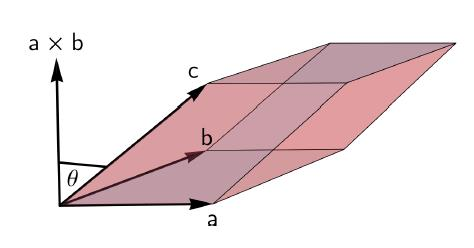
\includegraphics[width=\columnwidth]{cube.jpg}
\end{column}
\begin{column}{0.5\textwidth}
The volume is given by the base area
(the area of the parallelogram spanned by $a, b$) multiplied with the height, $|c||\cos\theta|$. Using the fact that $a\times b$ is orthogonal to $a$ and $b$ we have
\[|c|\cos\theta=\scp{\frac{a\times b}{|a\times b|}}{c},\]
\end{column}
\end{columns}
\vspace*{6pt}
so the volume is given by
\[V(a,b,c)=|a\times b|\left|\scp{\frac{a\times b}{|a\times b|}}{c}\right|=|\scp{a\times b}{c}|.\]
\end{spacing}
\end{frame}
\begin{frame}[t,shrink]{The Determinant in $\R^3$}
\begin{spacing}{1.1}
We therefore define the determinant as an \emph{oriented volume},
\begin{equation}\label{eq28}
  \det:\R^3\times\R^3\times\R^3\to\R,\qquad\det(a,b,c)=\scp{a\times b}{c}.
\end{equation}
(Again, we note that it can be equivalently defined $\text{Mat}(3\times 3;\R)\to\R$.) \\Note that
\begin{align}\label{eq29}
  \det(a,b,c)>0~~~ & \text{if}~(a,b,c)~\text{form a right-hand system,} \\
  \det(a,b,c)<0~~~ & \text{if}~(a,b,c)~\text{form a left-hand system,} \\
  \det(a,b,c)=0~~~ &\text{if}~a=\lambda b~\text{or}~a=\lambda c~\text{or}~b=\lambda c~\text{for any}~\lambda\in\R. \label{1.7.8}
\end{align}
The last property follows from the properties of the vector and scalar
products: if $a=\lambda b$ then $a\times b=0$, and since $a\times b$ is orthogonal both $a$ and $b$, the scalar product $\scp{a\times b}{c}$ will vanish if $a=\lambda c$ or $b=\lambda c$.
\end{spacing}
\end{frame}
\begin{frame}[c]{Cyclic Permutations}
\begin{spacing}{1.05}
Let $(x_1,\ldots,x_n)$ be an ordered list of elements. Define a relation $\prec$ by $x_1\prec x_2\prec x_3\prec\cdots\prec x_{n-1}\prec x_n\prec x_1$ ("$x_1$ precedes $x_2$ precedes $x_3$ etc."). Let $\pi:\{x_1,\ldots,x_n\}\to\{x_1,\ldots,x_n\}$ be a bijective map (such map is called a \emph{permutation}). Then any list $\left(\pi(x_1),\ldots,\pi(x_n)\right)$ is called a cyclic permutation of $(x_1,\ldots,x_n)$ if $\pi(x_1)\prec\pi(x_2)\prec\cdots\prec\pi(x_n)\prec\pi(x_1)$.\\
Furthermore, if $(a,b,c)$ form a right-hand system, then $V(a,b,c)=\det(a,b,c)$. Since the volume is independent of the
designation of the vectors, we observe that a \emph{cyclic permutation} of $(a,b,c)$ preserves the right-handedness and
\[\det(a,b,c)=\det(c,a,b)=\det(b,c,a)\]
or
\[\scp{a\times b}{c}=\scp{c\times a}{b}=\scp{b\times c}{a}.\]
\end{spacing}
\end{frame}
\begin{frame}[c,allowdisplaybreaks,allowframebreaks]{Calculating Determinants in $\R^3$}
\begin{spacing}{1}
Note that by \eqref{1.7.4},
\vspace*{-7pt}
\begin{equation}\label{1.7.9}
  \begin{split}
     \det(a,b,c) &=\scp{b\times c}{a}=\sum_{i=1}^{3}a_i(b\times c)_i \\
       &=a_1\det\begin{pmatrix}
                  b_2 & c_2 \\
                  b_3 & c_3
                \end{pmatrix}-a_2\begin{pmatrix}
                                   b_1 &c_1 \\
                                    b_3& c_3
                                 \end{pmatrix}+a_3\begin{pmatrix}
                                                    b_1 &c_1 \\
                                                    b_2 & c_2
                                                  \end{pmatrix}  \\
       &=\det\begin{pmatrix}
               a_1 & b_1 & c_1 \\
               a_2 & b_2 & c_2 \\
               a_3 & b_3 & c_3
             \end{pmatrix}
  \end{split}
\end{equation}
We may therefore calculate a $3\times 3$ determinant $\det A$ by calculating $2\times 2$
\emph{subdeterminants}. Denote by $A_{kj}$ the $2\times 2$ matrix obtained from $A$ by
deleting the $k$th row and the $j$th column, \eqref{1.7.9} can be written as
\begin{equation}\label{1.7.10}
  \det A=\det\begin{pmatrix}
               a_{11} & a_{12} & a_{13} \\
               a_{21} & a_{22} & a_{23} \\
               a_{31} & a_{32} & a_{33}
             \end{pmatrix}=\sum_{k=1}^{3}(-1)^{k+1}a_{k1}\det A_{k1}
\end{equation}
\newpage
We will prove later that in fact
\[\det\begin{pmatrix}
        a_1 & b_1 & c_1 \\
        a_2 & b_2 & c_2 \\
        a_3 & b_3 & c_3
      \end{pmatrix}=\det\begin{pmatrix}
                          a_1 & a_2 & a_3\\
                          b_1 & b_2 & b_3\\
                          c_1 & c_2 & c_3
                        \end{pmatrix}.\]
This (together with \eqref{1.7.9}) motivates the mnemonic
\[a\times b=\det\begin{pmatrix}
                  e_1 & e_2 & e_3 \\
                  a_1 & a_2 & a_3 \\
                  b_1 & b_2 & b_3
                \end{pmatrix},\]
where $e_1,e_2,e_3$ are the standard unit basis vectors and $a=(a_1,a_2,a_3)$,\\$b=(b_1,b_2,b_3)$.
\end{spacing}
\end{frame}
\begin{frame}[t]{Properties of the Determinant in $\R^3$}
\begin{spacing}{1.1}
We once more note the following properties of the determinant:
\begin{enumerate}[1.]
  \item det is \emph{normed}, i.e.,
  \[\det(e_1,e_2,e_3)=\det\begin{pmatrix}
                            1 & 0 & 0\\
                             0& 1 & 0\\
                            0 & 0 & 1
                          \end{pmatrix}=1.\]
  \item det is \emph{trilinear}:
  \begin{center}
    $\det(\lambda a,b,c)=\lambda\det(a,b,c)=\det(a,\lambda b,c)=\det(a,b,\lambda c)$,\\
    $\det(a+b,c,d)=\det(a,c,d)+\det(b,c,d)$,\\
    $\det(a,b+c,d)=\det(a,b,d)+\det(a,c,d)$,\\
    $\det(a,b,c+d)=\det(a,b,c)+\det(a,b,d)$
  \end{center}
  These properties follow from the correponding properties of the scalar and vector products.
  \item det is \emph{alternating} (see \eqref{1.7.8}).
\end{enumerate}
\end{spacing}
\end{frame}
\begin{frame}[c,allowdisplaybreaks,allowframebreaks]{Preview of Determinants in $\R^n$}
\begin{spacing}{1}
Our goal is now to find a generalization of the determinant that has the three main properties of being
\begin{itemize}
  \item multilinear,
  \item alternating and
  \item normed.
\end{itemize}
It will turn out that these three properties are actually suf{}ficient to define the determinant uniquely; there is only one map $\text{Mat}(n\times n;\R)\to\R$ with these properties, and for $n=2,3$ it is given by \eqref{eq27} and \eqref{eq28}, respectively.\\[6pt]
In the case of $n=1,\text{Mat}(1\times 1;\R)$ is equivalent to $\R$ and we define $\det(a)=a$. This definition trivially has the properties of being normed and linear; while it makes no sense to define what alternating means.
\newpage
We will further see that one possible formula for determinants $\det:\text{Mat}(n\times n)\to\R$ can be constructed recursively, similar to \eqref{1.7.10}.\\[6pt]
In fact, if $A\in\text{Mat}(n\times n;\R)$, we define $A_{kj}\in\text{Mat}((n-1)\times(n-1);\R)$ as the matrix obtained from $A$ by deleting the $k$th row and the $j$th column. Then for any $j=1,\ldots,n$ we will obtain the recursion formula
\begin{equation}\label{1.7.11}
  \det A=\sum_{k=1}^{n}(-1)^{k+j}a_{kj}\det A_{kj}
\end{equation}
In order to understand the extension of determinants to $\R^n$ better, we
need to formalize the concept of permutations.
\end{spacing}
\end{frame}
\begin{frame}[c]{Groups}
\begin{spacing}{1.3}
\alert{1.7.3. Definition.} A \emph{group} is a pair $(G,\circ)$ consisting of a set $G$ and a \emph{group operation} $\circ:G\times G\to G$ such that
\begin{itemize}
  \item[1.] $a\circ(b\circ c)=(a\circ b)\circ c$ for all $a,b,c\in G$(associativity),
  \item[2.] there exists an element $e\in G$ such that $a\circ e=e\circ a=a$ for all $a\in G$ (existence of a unit element),
  \item[3.] for every $a\in G$ there exists an element $a^{-1}\in G$ such that $a\circ a^{-1}=a^{-1}\circ a=e$ (existence of an inverse).
\end{itemize}
A group is called commutative if in addition to the above properties
\begin{itemize}
  \item[4.] $a\circ b=b\circ a$ for all $a,b\in G$ (commutativity).
\end{itemize}
\end{spacing}
\end{frame}
\begin{frame}[t,shrink]{Groups and Permutations}
\begin{spacing}{1.1}
\alert{1.7.4. Examples.}
\begin{enumerate}[1.]
  \item Any vector space $(V,+,\cdot)$ may be regarded as a commutative group $(V,+)$ with the additional operation of scalar multiplication.
  \item The set of invertible matrices,
      \[\text{GL}(n;\R):=\{A\in\text{Mat}(n\times n;\R):~A~\text{is invertible}\}\]
      is a group with the group operation given by matrix multiplication (composition of maps).
\end{enumerate}
\alert{1.7.5. Definition.} The set of all \emph{permutations of n elements}
\[S_n=\{\pi:\{x_1,\ldots,x_n\}\to\{x_1,\ldots,x_n\}:\pi~\text{bijective}\}\]
together with the group operation "composition of maps", $\pi_1\circ\pi_2(x)=\pi_1(\pi_2(x))$ is called the \emph{symmetric group}.
\end{spacing}
\end{frame}
\begin{frame}[c]{Permutations}
\begin{spacing}{1.1}
\begin{sloppypar}
It is easy to check that $(S_n,\circ)$ in fact has peroperties i)-iii), but not property iv). We will often denote a group by $G$ instead of $(G,\circ)$ if no confusion arises therefrom.\\[6pt]
A permutation of $n$ elements is a finite map; recall that a function $f$ is defined by pairs of the form $(x,f(x))$, where $x$ is the independent variable. A permutation is defined on a set of $n$ elements; instead of $\{x_1,\ldots,x_n\}$ we can also simply write $\{1,\ldots,n\}$, replacing the permutation $\pi$ through a set of pairs $\{(1,\pi(1)),\ldots,(n,\pi(n))\}$. In fact, we do represent permutations in this way, but us a dif{}ferent notation, writing
\end{sloppypar}
\[\pi=\begin{pmatrix}
1 & 2 & \cdots & n \\
\pi(1) & \pi(2) & \cdots & \pi(n)
\end{pmatrix}\]
\end{spacing}
\end{frame}
\begin{frame}[t,shrink]{Transpositions}
\begin{spacing}{1}
For example, if $n=2$, there are only two permutations $\pi_1,\pi_2\in S_2$,
\begin{equation}\label{1.7.12}
\begin{aligned}
\pi_{1}:1\mapsto 1,\qquad\qquad 2\mapsto 2,\qquad \pi_1&=\begin{pmatrix}1&2\\1&2\end{pmatrix},\\
\pi_{2}:1\mapsto 2,\qquad\qquad 2\mapsto 1,\qquad \pi_{2}&=\begin{pmatrix}1&2\\2&1\end{pmatrix}.
\end{aligned}
\end{equation}
\alert{1.7.6. Definition.} A permutation in $S_n$ that leaves exactly $n-2$ elements invariant is called a \emph{transposition}.\\[6pt]
A transposition $\tau\in S_n$ has the form
\begin{equation}\label{1.7.13}
\tau(k)=\left\{\begin{aligned}&i\qquad\text{if}~k=j\\
&j\qquad\text{if}~k=i\\
&k\qquad\text{otherwise}\end{aligned}\right.
\end{equation}
for some $i,j\in\{1,\ldots,n\}$.
\end{spacing}
\end{frame}
\begin{frame}[t,allowdisplaybreaks,allowframebreaks]{Permutations as Transpositions}
\begin{spacing}{1}
\alert{1.7.7. Lemma.} Every permutation $\pi\in S_n,n\geq2$, is a composition of transpositions, $\pi=\tau_1\circ\cdots\circ\tau_k$.\\[6pt]
Note that the transpositions $\tau_j$ and the number $k$ are \textcolor[rgb]{1.00,0.00,0.00}{not} uniquely defined.\\[5pt]
\alert{Proof.}\\
We proceed by induction. For $n=2$ there are only two permutations $\pi_1$ and $\pi_2$ (see \eqref{1.7.12}); $\pi_2$ is a transposition, and $\pi_1=\pi_2\circ\pi_2$. We now assume that any permutation in $S_n$ can be written as a composition of transpositions and prove that this is also true for any permutation in $S_{n+1}$.\\[7pt]
Let $\pi\in S_n$. Then we can consider
\begin{equation}\label{1.7.14}
  \widetilde{\pi}=\begin{pmatrix}
                    1 & \cdots & n & n+1 \\
                    \pi(1) & \cdots & \pi(n)& n+1
                  \end{pmatrix}
\end{equation}
as an element of $S_{n+1}$. Also, every element $\widetilde{\pi}\in S_{n+1}$ of the form \eqref{1.7.14} can be regarded as an element $\pi\in S_n$.
\newpage
\alert{Proof (continued).}\\
Now let $\sigma\in S_{n+1}$ and let $\tau$ be the transposition that exchanges $n+1$ and $\sigma^{-1}(n+1)$. Then
\[\sigma\circ\tau:n+1\xmapsto[]{\tau}\sigma^{-1}(n+1)\xmapsto[]{\sigma}n+1\]
so that
\[\sigma\circ\tau=\begin{pmatrix}
                    1 & \cdots & n & n+1 \\
                    \pi(1) & \cdots & \pi(n) & n+1
                  \end{pmatrix}\]
for some values $\pi(1),\ldots,\pi(n),\pi\in S_n$. It follows that $\sigma\circ\tau$ can be written as a composition of transpositions $\tau_1\circ\cdots\circ\tau_k$,
\[\sigma\circ\tau=\tau_1\circ\cdots\circ\tau_k,\]
so $\sigma=\tau_1\circ\cdots\circ\tau_k\circ\tau^{-1}$, which proves the assertion.
\begin{flushright}
  $\square$
\end{flushright}
\end{spacing}
\end{frame}
\begin{frame}[t,shrink]{Sign of a Permutation}
\begin{spacing}{1.2}
While the number of transpositions that make up a permutation is not
unique, we do have the following:\\
\alert{1.7.8. Definition and Theorem.} Let $\pi\in S_n$ be represented as a composition of $k$ transpositions, $\pi=\tau_1\circ\cdots\circ\tau_k$. Then the \emph{sign} of $\pi$,
\[\text{sgn}\,\pi:=(-1)^k\]
does not depend on the representation chosen.\\
In order to prove this, we need an additional concept from group theory,
which we introduce on the following slide.\\
In advance, we that the sign is "well-behaved":
\[\text{sgn}(\pi_1\circ\pi_2)=\text{sgn}\,\pi_1\,\text{sgn}\,\pi_2\]
for any $\pi_1,\pi_2\in S_n$.
\end{spacing}
\end{frame}
\begin{frame}[t,allowdisplaybreaks,allowframebreaks]{Group Actions}
\begin{spacing}{1.1}
\alert{1.7.9. Definition.} Let $(G,\circ)$ be a group and $X$ a set. Then an \emph{action (or operation) of G on X from the left} is a map
\[\Phi:G\times X\to X\qquad\qquad (g,x)\mapsto\Phi(g,x)=\Phi_g x=gx\]
with the properties
\begin{itemize}
  \item[1.] $ex=x$ ($e\in G$ is the unit element),
  \item[2.] $(a\circ b)x=a(bx)$ for $a,b\in G,x\in X$.
\end{itemize}
We say that $G$ acts (operates) on $X$.\\[10pt]
\alert{1.7.10. Proposition.} Let $X$ be the set of all maps $f:\R^n\to\R$. Then $S_n$ acts on $X$ via
\[(\pi f)(x_1,\ldots,x_n)=f(x_{\pi(1)},\ldots,x_{\pi(n)}),\qquad\qquad
\pi\in S_n.\]
\newpage
\alert{Proof.}\\
We need to show the properties i) and ii) of Definition 1.7.9. The unit
element of $S_n$ is
\[\pi_e=\begin{pmatrix}
          1 & \cdots & n \\
          1 & \cdots & n
        \end{pmatrix}\]
so trivially $\pi_ef=f$, since
\[(\pi_ef)(x_1,\ldots,x_n)=f(x_{\pi_e(1)},\ldots,x_{\pi_e(n)})=f(x_1,\ldots,x_n).\]
Furthermore, let $\sigma,\pi\in S_n$. Then
\begin{equation*}
  \begin{split}
     [\sigma(\pi f)](x) &=(\sigma f)(x_{\pi(1)},\ldots,x_{\pi(n)})=f(x_{\sigma(\pi(1))},\ldots,x_{\sigma(\pi(n))}) \\
       &=f(x_{(\sigma\circ\pi)(1)},\ldots,x_{(\sigma\circ\pi)(n)})=[(\sigma\circ\pi)f](x_1,\ldots,x_n),
  \end{split}
\end{equation*}
so $\sigma(\pi f)=(\sigma\circ\pi)f$.\multido{}{12}{\qquad}$\square$
\newpage
\alert{1.7.11. Lemma.} Denote by $\Delta:\R^n\to\R$ the function
\begin{equation}\label{1.7.15}
  \Delta(x_1,\ldots,x_n)=\prod_{i<j}(x_j-x_i).
\end{equation}
Then
\[\tau\Delta=-\Delta\qquad\qquad\qquad\text{for any transposition}~\tau\in S_n.\]
 \\[12pt]
\alert{Proof.}\\
Let $r,s\in\{1,\ldots,n\},r<s,$ and $\tau$ the transposition exchanging $r$ and $s$,
\begin{equation*}
\tau=\begin{pmatrix}
       1 & \cdots & r-1 & r & r+1 & \cdots & s-1 & s & s+1 & \cdots & n \\
        1& \cdots & r-1 & s & r+1 & \cdots & s-1 & r & s+1 & \cdots & n
     \end{pmatrix}
\end{equation*}
\newpage
\alert{Proof (continued).}\\
Note that
\[\tau\Delta(x_1,\ldots,x_n)=\prod_{i<j}\tau(x_j-x_i).\]
Then
\begin{equation}\label{1.7.16}
  \tau(x_r-x_s)=-(x_r-x_s).
\end{equation}
All other factors in \eqref{1.7.15} either do not contain $x_r$ or $x_s$ (and are left unchanged by $\tau$) or occur in one of the following pairings:
\begin{itemize}
  \item $j<r:(x_r-x_j)(x_s-x_j)$
  \item $r<j<s:(x_s-x_j)(x_j-x_r)$
  \item $s<j:(x_j-x_s)(x_j-x_r)$
\end{itemize}
Each of these pairs is left invariant by $\tau$, so the sign change in \eqref{1.7.16} is the only ef{}fect of $\tau$ on $\Delta$.
\end{spacing}
\end{frame}
\begin{frame}[t,shrink]{Sign of a Permutation}
\begin{spacing}{1}
\alert{1.7.12. Corollary.} For every permutation $\pi=\tau_1\circ\cdots\circ\tau_k\in S_n$,
\[\pi\Delta=(\tau_1\circ\cdots\circ\tau_k)\Delta=(-1)^k\Delta.\]
In particular,
\[\text{sgn}\,\pi=(-1)^k,\]
does not depend on the decomposition of $\pi$ into transpositions and is
therefore well-defined.\\[9pt]
\alert{Proof.}\\
Let $\pi\in S_n$ and assume that there are transpositions $\tau_1,\ldots,\tau_k,\widetilde{\tau_1},\ldots,\widetilde{\tau_l}$ such that
\[\pi=\tau_1\circ\cdots\circ\tau_k=\widetilde{\tau_1}\circ\cdots\circ\widetilde{\tau_l}.\]
Then $\pi\Delta(x_1,\ldots,x_n)=(-1)^k\Delta(x_1,\ldots,x_n)=(-1)^l\Delta(x_1,\ldots,x_n)$. Choosing some \myseries{x}{n} such that $\Delta(x_1,\ldots,x_n)\neq0$ we obtain $(-1)^k=(-1)^l$.
\end{spacing}
\end{frame}
\begin{frame}[t,shrink]{$p$-Multilinear Maps}
\begin{spacing}{1.05}
\alert{1.7.13. Definition.} A function $f:\underbrace{\R^n\times\cdots\times\R^n}_{p ~\text{times}}\to\R$ is said to be a \emph{p-multilinear map} (or \emph{p-multilinear form}) if $f$ is linear in each entry, i.e.,
\[f(\lambda a_1,a_2,\ldots,a_p)=\lambda f(a_1,a_2,\ldots,a_p)\]
and
\[f(a_1+b,a_2,\ldots,a_p)=f(a_1,a_2,\ldots,a_p)+f(b,a_2,\ldots,a_p)\]
for $b,a_1,\ldots,a_p\in\R^n$ and $\lambda\in\R$ and analogous equations hold for the other entries.\\[7pt]
The form is said to be \emph{alternating} if $f(a_1,\ldots,a_p)=0$ whenever $a_j=a_k$ for any $j\neq k$.\\
An $n$-multilinear form is said to be \emph{normed} if $f(e_1,\ldots,e_n)=1$, where \myseries{e}{n} are the standard basis vectors in $\R^n$.
\end{spacing}
\end{frame}
\begin{frame}[c]{Characterization of Alternating Forms}
\begin{spacing}{1.05}
We will prove that the properties of being multilinear, alternating and
normed are suf{}ficient to uniquely define the determinant in $\R^n$. First, however, we give a useful result:\\[5pt]
\alert{1.7.14. Lemma.} Let $f:\underbrace{\R^n\times\cdots\times\R^n}_{p ~\text{times}}\to\R$ be a $p$-multilinear map. Then the following are equivalent:
\begin{itemize}
  \item[(i)] $f$ is alternating
  \item[(ii)] $f(a_1,\ldots,a_{j-1},a_j,a_{j+1},\ldots,a_{k-1},a_k,a_{k+1},\ldots,a_p)$\\ \begin{flushright}
         $=-f(a_1,\ldots,a_{j-1},a_k,a_{j+1},\ldots,a_{k-1},a_j,a_{k+1},\ldots,a_p)$
      \end{flushright}
  \item[(iii)] $f(a_1,\ldots,a_p)=0$ if \myseries{a}{p} are linearly dependent.
\end{itemize}
The proof is not dif{}ficult and left as an exercise!
\end{spacing}
\end{frame}
\begin{frame}[c,allowdisplaybreaks,allowframebreaks]{Determinants in $\R^n$}
\begin{spacing}{1.05}
We will now define the determinant as an alternating, normed,
$n$-multilinear function for column vectors in $\R^n$ and corresponding square
matrices whose columns consist of these vectors, using the notation
\[a_j=\begin{pmatrix}
        a_{1j} \\
        \vdots \\
        a_{nj}
      \end{pmatrix},\qquad(j=1,\ldots,n),\qquad A=(a_1,\ldots,a_n)=\begin{pmatrix}
                           a_{11} & a_{12} & \cdots & a_{1n} \\
                           \vdots & \vdots &  & \vdots \\
                           a_{n1} & a_{n2} & \cdots & a_{nn}
                         \end{pmatrix}\]
\alert{1.7.15. Theorem.} For every $n\in\N,n>1$, there exists a unique, normed, alternating $n$-multilinear form det:$\underbrace{\R^n\times\cdots\times\R^n}_{n~\text{times}}\cong\text{Mat}(n\times n;\R)\to\R$.\\[7pt]
Furthermore,
\begin{equation}\label{1.7.17}
  \det(a_1,\ldots,a_n)=\det A=\sum_{\pi\in S_n}\text{sgn}\,\pi a_{\pi(1)1}\cdots a_{\pi(n)n},
\end{equation}
\newpage
\alert{Proof.}\\
We will first show that the determinant defined in \eqref{1.7.17} in fact has the required properties.
\begin{itemize}
  \item[1.] (det is multilinear) Let $a_1,\ldots,a_n,b\in\R^n$. Then we show the
additivity in the first entry (the proof for all other entries is completely analogous)
\begin{align*}
    &~\det(a_1+b,a_2,\ldots,a_n) \\
   &=\sum_{\pi\in S_n}\text{sgn}~\pi(a_{\pi(1)1}+b_{\pi(1)})a_{\pi(2)2}\cdots a_{\pi(n)n}  \\
   &=\sum_{\pi\in S_n}\text{sgn}~\pi a_{\pi(1)1}\cdots a_{\pi(n)n}+\sum_{\pi\in S_n}\text{sgn}~\pi b_{\pi(1)}\cdots a_{\pi(n)n}  \\
   &=\det(a_1,a_2,\ldots,a_n)+\det(b,a_2,\ldots,a_n)
\end{align*}
The homogeneity is shown analogously.
\end{itemize}
\newpage
\vspace*{20pt}
\alert{Proof (continued).}\\
\begin{itemize}
  \item[2.] (det is normed) Let
  \[e_j=\begin{pmatrix}
          \delta_{1j} \\
          \vdots \\
          \delta_{nj}
        \end{pmatrix}\qquad (j=1,\ldots,n),\qquad\qquad \delta_{ij}=\left\{\begin{aligned}1~~~&i=j,\\ 0~~~&i\neq j.\end{aligned}\right.\]
  Then for any permutation $\pi\in S_n$,
  \[\delta_{1\pi(1)}\cdots\delta_{n\pi(n)}=\left\{\begin{aligned}1~~~&\pi(k)=k,~k=1,\ldots,n,\\
  0~~~&\text{otherwise.}\end{aligned}\right.\]
\end{itemize}
\newpage
\vspace*{18pt}
\alert{Proof (continued).}\\
\begin{itemize}
  \item[2.] It follows that in the summation of the permutations only the summand with
      \[\pi=\begin{pmatrix}
              1 & 2 & \cdots & n-1 & n \\
              1 & 2 & \cdots & n-1 & n
            \end{pmatrix},\qquad\qquad\text{sgn}\,\pi=1,\]
      survives. Thus
      \[\det(e_1,\ldots,e_n)=\sum_{\pi\in S_n}\text{sgn}\,\pi\delta_{\pi(1)1}\cdots\delta_{\pi(n)n}=1.\]
\end{itemize}
\newpage
\vspace*{20pt}
\alert{Proof (continued).}\\
\begin{itemize}
  \item[3.] (det is alternating) We will show that $\det(a_1,a_2,\ldots,a_{n-1},a_n)=-\det(a_n,a_2,\ldots,a_{n-1},a_1)$ (again, the proof is similar when any other entries are exchanged). Let
      \begin{equation}\label{1.7.18}
        \tau=\begin{pmatrix}
               1 & 2 & \cdots & n-1 & n \\
               n & 2 & \cdots & n-1 & 1
             \end{pmatrix}\in S_n.
      \end{equation}
      be be the transposition exchanging 1 and $n$. We will use that $\text{sgn}\,\tau=-1$
      and that summing over all permutations $\pi\in S_n$ is the same as summing over all $\tau\circ\pi\in S_n$, when $\tau$ is fixed by \eqref{1.7.18}.
\end{itemize}
\newpage
\vspace*{20pt}
\alert{Proof (continued).}\\
\begin{itemize}
  \item[3.] Then
  \begin{equation*}
    \begin{split}
         &~\det(a_n,a_2,\ldots,a_{n-1},a_1)  \\
         &=\sum_{\pi\in S_n}\text{sgn}\,\pi a_{\pi(1)n}a_{\pi(2)2}\cdots a_{\pi(n-1)(n-1)}a_{\pi(n)1}  \\
         &=\sum_{\pi\in S_n}\text{sgn}\,\pi a_{\pi(n)1}a_{\pi(2)2}\cdots a_{\pi(n-1)(n-1)}a_{\pi(1)n}  \\
         &=-\sum_{\tau\circ\pi\in S_n}\text{sgn}(\tau\circ\pi)a_{\tau\circ\pi(1)1}a_{\tau\circ\pi(2)2}\cdots a_{\tau\circ\pi(n-1)(n-1)}a_{\tau\circ\pi(n)n}  \\
         &=\det(a_1,a_2,\ldots,a_{n-1},a_n).
    \end{split}
  \end{equation*}
\end{itemize}
\newpage
\alert{Proof (continued).}\\
We next show that the properties of the determinant imply the formula \eqref{1.7.17}. By multilinearity we have
\begin{equation*}
  \begin{split}
     \det(a_1,\ldots,a_n) &=\det\left(\sum_{j_1=1}^{n}a_{j_11}e_{j_1},\ldots,\sum_{j_n=1}^{n}a_{j_nn}e_{j_n}\right) \\
       &=\sum_{j_1,\ldots,j_n=1}^{n}a_{j_11}\cdots a_{j_nn}\det(e_{j_1},\ldots,e_{j_n})
  \end{split}
\end{equation*}
Since det is supposed to be alternating, all summands vanish where any $j_k$ occurs more than once. We therefore sum only over permutations of
$\{1,\ldots,n\}$,
\[\det(a_1,\ldots,a_n)=\sum_{\pi\in S_n}a_{\pi(1)1}\cdots a_{\pi(n)n}\det(e_{\pi(1)},\ldots,e_{\pi(n)})\]
\newpage
\alert{Proof (continued).}\\
Again, because det is alternating and assuming each $\pi$ is composed of $k$ transpositions,
\[\det(e_{\pi(1)},\ldots,e_{\pi(n)})=(-1)^{k}\det(e_1,\ldots,e_n)=\text{sgn}\,\pi\det(e_1,\ldots,e_n).\]
Since det is normed, $\det(e_1,\ldots,e_n)=1$, so we finally have
\[\det(a_1,\ldots,a_n)=\sum_{\pi\in S_n}a_{\pi(1)1}\cdots a_{\pi(n)n}\,\text{sgn}\,\pi.\]
\begin{flushright}
  $\square$
\end{flushright}
\end{spacing}
\end{frame}
\begin{frame}[t]{Determinant and Elementary Column Operations}
\begin{spacing}{1.05}
Since the determinant is alternating and multilinear, we see that the
Elementary Column Operations 1.5.8 af{}fect the determinant as follows:
\begin{itemize}
  \item The determinant of a matrix $A$ changes sign if two columns of $A$ are interchanged, e.g.,
      \[\det(a_2,a_1,\ldots,a_n)=-\det(a_1,a_2,\ldots,a_n)\]
  \item Multiplying all the entries in a column with a number $\lambda$ leads to the determinant being multiplied by this constant:
      \[\det(a_1,\ldots,\lambda a_j,\ldots,a_n)=\lambda\det(a_1,\ldots,a_j,\ldots,\ldots,a_n)\]
  \item Adding a multiple of a column to another column does not change the value of the determinant:
      \[\det(a_1,\ldots,a_j,\ldots,a_k+\lambda a_j,\ldots,a_n)=\det(a_1,\ldots,a_j,\ldots,a_k,\ldots,a_n)\]
\end{itemize}
\end{spacing}
\end{frame}
\begin{frame}[t]{Determinants of Transposed Matrices}
\begin{spacing}{1.05}
\alert{1.7.16. Lemma.} Let $A\in\text{Mat}(n\times n;\R)$. Then
\[\det A=\det A^T,\]
 \\[9pt]
\alert{Proof.}\\
We first note that for every $\pi\in S_n,\text{sgn}\,\pi=\text{sgn}\,\pi^{-1}$ and the sum over all $\pi$ is equal to the sum over all $\pi^{-1}$. Then we can reorder the terms in each summand, so that
\begin{equation*}
  \begin{split}
     \det A &=\sum_{\pi\in S_n}\text{sgn}\,\pi a_{\pi(1)1}\cdots a_{\pi(n)n}=\sum_{\pi\in S_n}\text{sgn}\,\pi a_{1\pi^{-1}(1)}\cdots a_{n\pi^{-1}(n)} \\
       &=\sum_{\pi^{-1}\in S_n}\text{sgn}\,\pi^{-1}a_{1\pi^{-1}(1)}\cdots a_{n\pi^{-1}(n)}=\sum_{\pi\in S_n}\text{sgn}\,\pi a_{1\pi(1)}\cdots a_{n\pi(n)}  \\
       &=\det A^T.
  \end{split}
\end{equation*}
\begin{flushright}
  $\square$
\end{flushright}
\end{spacing}
\end{frame}
\begin{frame}[t]{Determinants and Elementary Row Operations}
\begin{spacing}{1.05}
As a corollary, we can rewrite \eqref{1.7.17} in a more commonly seen form:\\
\alert{1.7.17. Leibnitz Formula.}
\begin{equation}\label{1.7.19}
  \det A=\sum_{\pi\in S_n}\text{sgn}\,\pi a_{1\pi(1)}\cdots a_{n\pi(n)}
\end{equation}
\alert{1.7.18. Corollary.} Elementary row manipulations of a matrix $A$ af{}fect the
determinant of $A$ in the same way as the corresponding elementary column
manipulations.\\[6pt]
\alert{Proof.}
\[
\begin{CD}
\det{A} @>{\text{row manipulation}}>{}> \det{B}\\
@| @| \\
\det{A^T} @>{\text{column manipulation}}>{}> \det{B^T}
\end{CD}
\]
\begin{flushright}
  $\square$
\end{flushright}
\end{spacing}
\end{frame}
\begin{frame}[c,allowdisplaybreaks,allowframebreaks]{Triangular Determinants}
\begin{spacing}{1.05}
\vspace*{19pt}
\alert{1.7.19. Proposition.} Let $A\in\text{Mat}(n\times n)$ have upper triangular form, i.e.,
\[A=\begin{pmatrix}
      \lambda_1 &  & * \\
       & \ddots &  \\
      0 &   & \lambda_n
    \end{pmatrix}\]
for diagonal elements \myseries{\lambda}{n}$\in\R$ and arbitrary values (denoted by $*$) above the diagonal. Then
\vspace*{13pt}
\[\det A=\lambda_1\cdots\lambda_n.\]
\newpage
\alert{Proof.}\\
By multilinearity,
\[\det A=\left(\prod_{i=k}^{n}\lambda_k\right)\det\begin{pmatrix}
                                             1 &  & * \\
                                              & \ddots &  \\
                                             0 &  & 1
                                           \end{pmatrix}.\]
The matrix in the determinant on the right can be transformed into the
unit matrix through elementary row manipulations that do not change the
value of the determinant. Therefore its determinant is 1, proving the
result.
\begin{flushright}
  $\square$
\end{flushright}
%\vspace*{7pt}
Proposition 1.7.19 can be applied to calculate determinants of matrices $A\in\text{Mat}(n\times n)$ when $A$ is first transformed to upper triangular form using elementary matrix manipulations. This is of practical use for $n\geq 4$.
\end{spacing}
\end{frame}
\begin{frame}[t]{Determinants and Invertibility of Matrices}
\begin{spacing}{1.05}
The following result is of fundamental importance for many applications:\\[7pt]
\alert{1.7.20. Proposition.} A matrix $A\in\text{Mat}(n\times n)$ is invertible if and only if $\det A\neq 0$.\\[8pt]
\alert{Proof.}\\
We first show that if $A$ is not invertible, then $\det A=0$. The linear map $A:\R^n\to\R^n$ is invertible if and only if $\text{ran}\,A=\R^n$. Since $\text{ran}\,A$ is the span of the column vectors, $A$ is invertible if and only if the column vectors are independent. But if the column vectors are not independent, then $\det A$ vanishes.\\[7pt]
Now let $A=(a_1,\ldots,a_n)$ be invertible. By Lemma 1.5.13 $A$ can be transformed into the unit matrix by elementary row operations. These only change the value of the determinant by a non-zero factor. Since the determinant of the unit matrix is 1, it follows that $\det A\neq 0$.
\begin{flushright}
  $\square$
\end{flushright}
\end{spacing}
\end{frame}
\begin{frame}[t,allowdisplaybreaks,allowframebreaks]{Determinants and Systems of Equations}
\begin{spacing}{1.05}
The determinant can be used to give another formulation of Fredholm's
Alternative 1.6.4:\\[6pt]
\alert{1.7.21. Fredholm Alternative.} Let $A\in\text{Mat}(n\times n).$ Then either
\begin{itemize}
  \item $\det A=0$, in which case $Ax=0$ has a non-zero solution $x\in\ker A$, or
  \item $\det A\neq0$, then $Ax=b$ has a unique solution $x=A^{-1}b$ for any $b\in\R^n$.
\end{itemize}
The proof is a straightforward application of the definitions and left to the reader.\\[6pt]
\alert{1.7.22. Cramer's Rule.} Let $A=(a_1,\ldots,a_n)\in\text{Mat}(n\times n),\,a_1,\ldots,a_n\in\R^n$ be invertible. Then the system $Ax=b,b\in\R^n$ has the solution
\begin{equation}\label{1.7.20}
  x_i=\frac{1}{\det A}\det(a_1,\ldots,a_{i-1},b,a_{i+1},\ldots,a_n),\qquad i=1,\ldots,n.
\end{equation}
\newpage
\alert{Proof.}\\
We note that $Ax=\sum\limits_{k=1}^{n}x_ka_k$ for $A=(a_1,\ldots,a_n)\in\text{Mat}(n\times n)$. Therefore,
\begin{equation*}
  \begin{split}
       &~~~~~\det(a_1,\ldots,a_{i-1},b,a_{i+1},\ldots,a_n)  \\
       &=\det(a_1,\ldots,a_{i-1},Ax,a_{i+1},\ldots,a_n)  \\
       &=\det\left(a_1,\ldots,a_{i-1},\sum_{k=1}^{n}x_ka_k,a_{i+1},\ldots,a_n\right)  \\
       &=\sum_{k=1}^{n}x_k \det(a_1,\ldots,a_{i-1},a_k,a_{i+1},\ldots,a_n)  \\
       &=x_i\det(a_1,\ldots,a_{i-1},a_i,a_{i+1},\ldots,a_n)+0  \\
       &=x_i\det A.
  \end{split}
\end{equation*}
\begin{flushright}
  $\square$
\end{flushright}
\end{spacing}
\end{frame}
\begin{frame}[t]{Minors and Cofactors}
\begin{spacing}{1}
\alert{1.7.23. Definition.} Let $A=(a_{ij})\in\text{Mat}(n\times n)$. Denote the $(n-1)\times (n-1)$ matrix obtained from $A$ by deleting the $i$th row and $j$th column by
\[A_{ij}=(a_{kl})_{\begin{subarray}~1\leq k,l\leq n.\\ ~~~k\neq i\\ ~~~l\neq j\end{subarray}}\]
Then
\[m_{ij}:=\det A_{ij}\]
is called the $(i,j)$\emph{th minor of A}. The number
\[c_{ij}:=(-1)^{i+j}m_{ij}=(-1)^{i+j}\det A_{ij}\]
is called the $(i,j)$\emph{th cofactor of A} and the matrix
\[\text{Cof}\,A:=(c_{ij})_{1\leq i,j\neq n}\]
is called the \emph{cofactor matrix of A}.
\end{spacing}
\end{frame}
\begin{frame}[c,allowdisplaybreaks,allowframebreaks]{Determinants and Inversion of Matrices}
\begin{spacing}{1.1}
\vspace*{18pt}
\alert{1.7.24. Definition.} Let $A=(a_{ij})\in\text{Mat}(n\times n)$. The transpose of the cofactor matrix of $A$ is called the \emph{adjugate} of $A$, denoted by
\[A^{\sharp}:=(\text{Cof}\,A)^T\]
 \\[9pt]
\alert{1.7.25. Theorem.} Let $A=(a_{ij})\in\text{Mat}(n\times n)$ be invertible. Then
\[A^{-1}=\frac{1}{\det A}A^{\sharp}\]
The proof is based on a useful lemma, which we first establish.
\newpage
\vspace*{14pt}
\alert{1.7.26. Lemma.} Let $A=(a_1,\ldots,a_n)\in\text{Mat}(n\times n)$ and $e_i$ be the $i$th standard basis vector in $\R^n$. Then
\[\det(a_1,\ldots,a_{j-1},e_i,a_{j+1},\ldots,a_n)=(-1)^{i+j}\det A_{ij}=c_{ij}\]
where $c_{ij}$ is the $(i,j)$th cofactor of $A$.\\[8pt]
\alert{Proof.}\\
Since the determinant is multilinear, we have
\begin{equation*}
  \begin{split}
       &~~~\det(a_1,\ldots,a_{j-1},e_i,a_{j+1},\ldots,a_n)  \\
       &=-\det(a_1,\ldots,a_{j-1},a_{j+1},e_i,a_{j+2},\ldots,a_n)  \\
       &=(-1)^{n-j-1}\det(a_1,\ldots,a_{j-1},a_{j+1},\ldots,a_n,e_i).
  \end{split}
\end{equation*}
\newpage
\vspace*{15pt}
\alert{Proof (continued).}\\
Swapping $i$th and the $(i+1)$st row, etc., we obtain
\begin{equation*}
  \begin{split}
     \det(a_1,\ldots,a_{j-1},e_i,a_{j+1},\ldots,a_n) &=(-1)^{n-j-1+n-i-1}\det\begin{pmatrix}
                               A_{ij} & 0 \\
                               * & 1
                             \end{pmatrix} \\
       &=(-1)^{i+j}\det B.
  \end{split}
\end{equation*}
where the entries in $*$ represent the elements of the $i$th row of $A$ (with the
$j$th entry deleted). Now from the definition (1.7.17),
\begin{equation*}
  \det\begin{pmatrix}
        A_{ij} & 0 \\
        * & 1
      \end{pmatrix}=\det B=\sum_{\pi\in S_n}\text{sgn}\,\pi b_{\pi(1)1}\cdots b_{\pi(n)n}
\end{equation*}
\newpage
\alert{Proof (continued).}\\
Since $b_{\pi(n)n}=\delta_{n\pi(n)}$, we can write
\[\det\begin{pmatrix}
        A_{ij} & 0 \\
        * & 1
      \end{pmatrix}=\det B=\sum_{\pi\in S_{n-1}}\text{sgn}\,\pi b_{\pi(1)1}\cdots b_{\pi(n-1)(n-1)}\underbrace{b_{nn}}_{=1}=\det A_{ij},\]
complete the proof.\multido{}{12}{\qquad}\quad{$\square$}\\
\alert{Proof of Theorem 1.7.25.}\\
Let $A^{-1}=(x_1,\ldots,x_n)=(x_{ij})$ be a matrix of column vectors \myseries{x}{n}. The inverse of $A$ satisfies $AA^{-1}=\text{id}$, so we need to find columns $x_j$ of $A^{-1}$ satisfying $Ax_j=e_j,j=1,\ldots,n$.\\[4pt]
By Cramer's rule and Lemma 1.7.26,
\begin{equation*}
x_{ij}=\frac{1}{\det A}\det(a_1,\ldots,a_{i-1},e_j,a_{i+1},\ldots,a_n)=\frac{1}{\det A}(-1)^{i+j}A_{ji}.\qquad\qquad\square
\end{equation*}
\end{spacing}
\end{frame}
\begin{frame}[t,allowdisplaybreaks,allowframebreaks]{Laplace Expansion}
\begin{spacing}{1.05}
Another application of Lemma 1.7.26 is the expansion of $\det A$ in terms of
the minors of A:\\[5pt]
\alert{1.7.27. Laplace Expansion.} For $A\in\text{Mat}(n\times n)$ and any $j=1,\ldots,n$ the recursion formula
\begin{equation}\label{1.7.21}
  \det A=\sum_{i=1}^{n}(-1)^{i+j}a_{ij}\det A_{ij}
\end{equation}
holds.\\[6pt]
Note that when using this expansion to calculate the determinant of an $n\times n$ matrix, $n$ determinants of $(n-1)\times(n-1)$ matrices need to be
evaluated. This means the number of computational steps required is
much larger than when Proposition 1.7.19 is used.
\newpage
\alert{Proof.}\\
Let $A=(a_1,\ldots,a_n),a_k\in\R^n,k=1,\ldots,n$. Then the $j$th column has the representation $a_j=\sum_{i=1}^{n}a_{ij}e_i$ and
\begin{equation*}
  \begin{split}
     \det A &=\det\left(a_1,\ldots,a_{j-1},\sum_{i=1}^{n}a_{ij}e_i,a_{j+1},\ldots,a_n\right) \\
       &=\sum_{i=1}^{n}a_{ij}\det\left(a_1,\ldots,a_{j-1},e_i,a_{j+1},\ldots,a_n\right)  \\
       &=\sum_{i=1}^{n}a_{ij}(-1)^{i+j}\det A_{ij},
  \end{split}
\end{equation*}
where the last equality follows from Lemma 1.7.26.
\begin{flushright}
  $\square$
\end{flushright}
\end{spacing}
\end{frame}
\begin{frame}[t,allowdisplaybreaks,allowframebreaks]{Determinants and Minors}
\begin{spacing}{1.1}
\includegraphics[scale=0.05]{mathematica.jpg}~We can obtain the determinant of a matrix as follows:
\begin{figure}
  \centering
  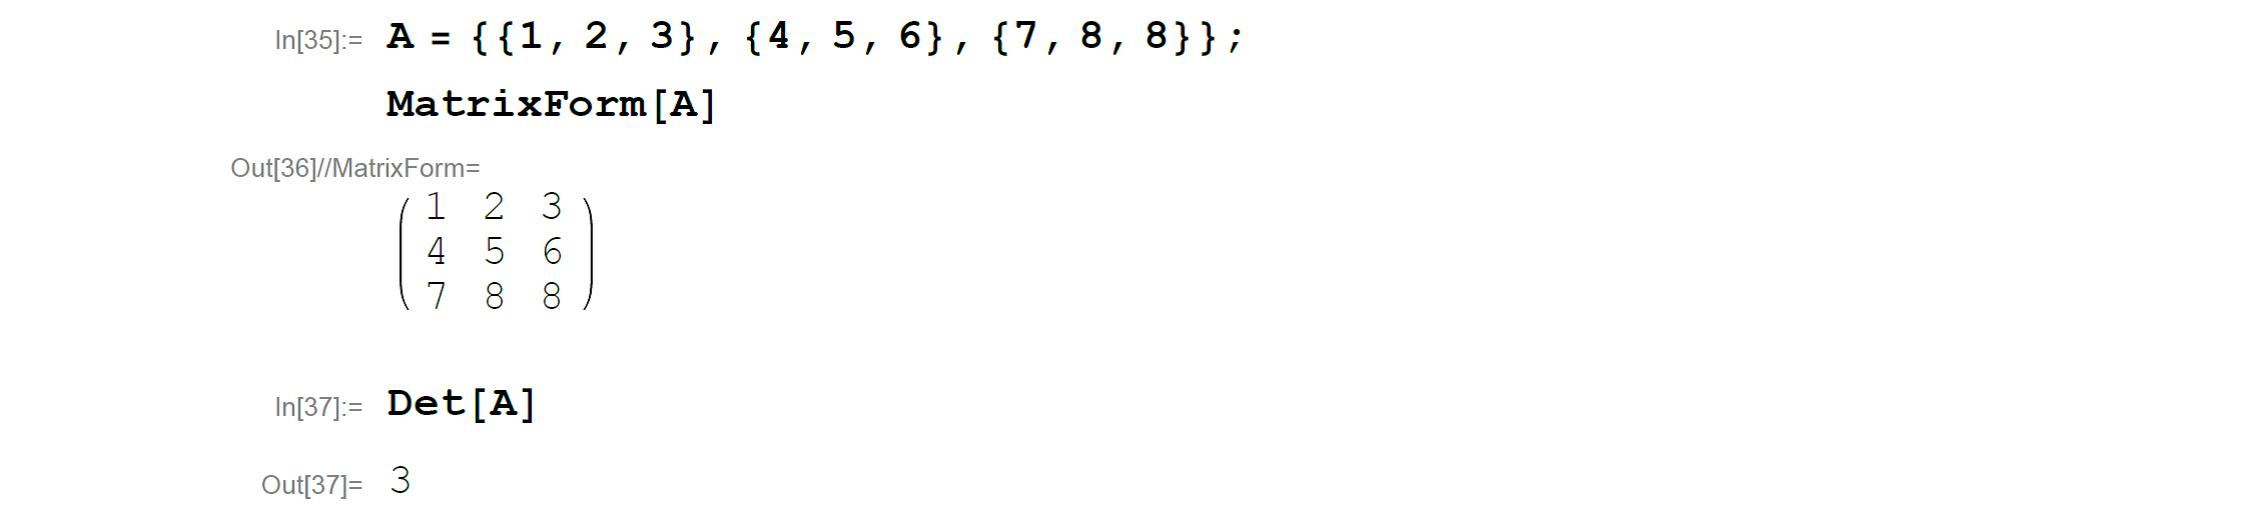
\includegraphics[width=\textwidth]{39.jpg}

\end{figure}
The Mathematica command \mathematicafont{\textbf{Minors}}~gives the matrix of minors of $A$.
However, the command returns the determinants of the submatrix found
by deleting the $(n-i-1)$th row and $(m-j-1)$th column. To conform
to our definition, the command needs to be modified slightly.
\newpage
\begin{figure}
  \centering
  
\includegraphics[width=\textwidth]{40.jpg}

\end{figure}
The adjugate matrix can be defined as follows:
\begin{figure}
  \centering
  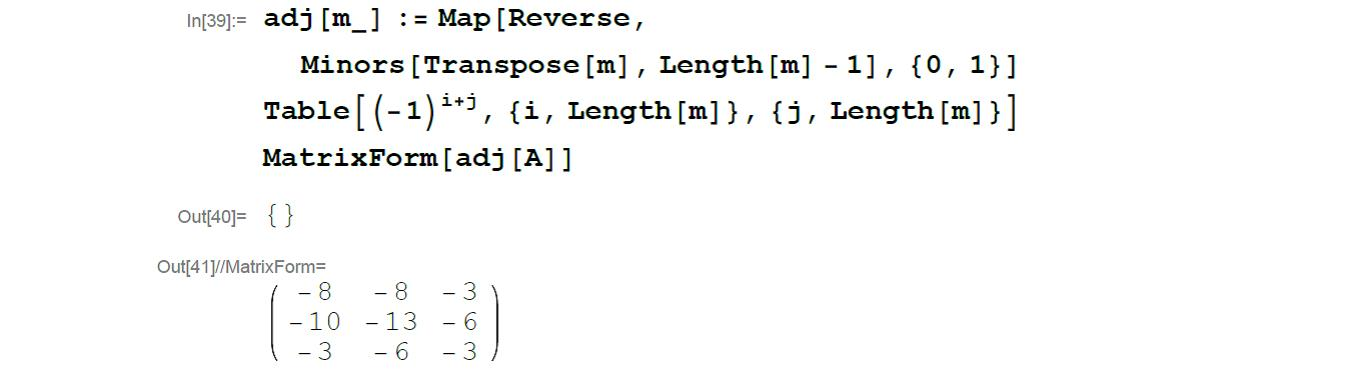
\includegraphics[width=\textwidth]{41.jpg}

\end{figure}
\end{spacing}
\end{frame}
\begin{frame}[t,allowdisplaybreaks,allowframebreaks]{Product Rule for Determinants}
\begin{spacing}{1.1}
\alert{1.7.28. Proposition.} Let $A,B\in\text{Mat}(n\times n)$. Then $\det(AB)=\det A\det B$.\\[6pt]
\alert{Proof.}\\
If $A=(a_{ik}),B=(b_{kj})$ then $AB=C=(c_{ij})$ with column vectors $c_j$,
\[c_j=\begin{pmatrix}
        c_{1j} \\
        \vdots \\
        c_{nj}
      \end{pmatrix},\qquad\qquad\qquad c_{ij}=\sum_{k=1}^{n}a_{ik}b_{kj}.\]
Let $b_j$ denote the columns of $B$, then
\[c_j=Ab_j.\]
We can assume that $A$ is invertible (otherwise $\det(AB)=0=\det A\det B$). Therefore $A$ is a bijective map.
\newpage
\alert{Proof (continued).}\\
Hence we can write
\begin{equation*}
  \begin{split}
     \det AB &=\det(c_1,\ldots,c_n)=\det(Ab_1,\ldots,Ab_n) \\
       &=\det(A(\cdot),\ldots,A(\cdot))[b_1,\ldots,b_n]=:f(b_1,\ldots,b_n)
  \end{split}
\end{equation*}
The so defined function $f$ is clearly multilinear. It is also alternating, because $A$ is bijective ($Ab_k=Ab_j$ if and only if $b_k=b_j,j,k=1,\ldots,n$). We will now norm $f$ by considering
\[\frac{1}{f(e_1,\ldots,e_n)}f(\cdot)=\frac{1}{\det A}f(\cdot),\]
Now the function $\frac{1}{\det A}f(\cdot)$ is multilinear, normed and alternating. Therefore, by the uniqueness of the determinant, it must be the determinant.
\newpage
\vspace*{18pt}
\alert{Proof (continued).}\\
That means that
\[\frac{1}{\det A}f(B)=\det B\qquad\qquad\qquad\Leftrightarrow\qquad\qquad\qquad f(B)=\det A\det B.\]
Since $f(B)$ was defined as $\det AB$, this proves the assertion.
\begin{flushright}
  $\square$
\end{flushright}
\alert{1.7.29. Corollary.} Let $A\in\text{Mat}(n\times n)$ be invertible. Then
\[\det A^{-1}=\frac{1}{\det A}.\]
\end{spacing}
\end{frame}
\begin{frame}[c]{First Midterm Exam}
The preceding material completes the first third of the course material. It
encompasses everything that will be the subject of the \textcolor[rgb]{1.00,0.00,0.00}{First Midterm Exam}.\\[8pt]
The exam date will be posted on SAKAI.\\[8pt]
No calculators or other aids will be permitted during the exam. A sample
exam with solutions has been uploaded to SAKAI. Please study it carefully,
including the instructions on the cover page.
\end{frame}
\section{Dif{}ferential Calculus}
\begin{frame}[c]
\begin{center}
  \Huge{Part II}\\ \alert{Dif{}ferential Calculus}
\end{center}
\end{frame}
\begin{frame}[c] \begin{spacing}{2.5}
\tableofcontents[hideothersubsections,sectionstyle=hide] \end{spacing}
\end{frame}
\subsection{Convergence and Continuity}
\begin{frame}[c]
\begin{spacing}{2.5}
\tableofcontents[sectionstyle=hide,subsectionstyle=show/shaded/hide]
\end{spacing}
\end{frame}
\begin{frame}[t,shrink]{Finite-Dimensional Vector Spaces}
\begin{spacing}{1}
For the rest of the term, we will focus on functions of several variables, e.g., functions
\[f:\R^n\to\R^m.\]
Our previously developed knowledge of linear algebra is essential for this,
since, for example, the derivative of such a function at a point x turns out
to be a matrix. More precisely, the derivative is a map
\[Df:\R^n\to\text{Mat}(m\times n;\R).\]
It is not suf{}ficient to restrict ourselves to functions defined on $\R^n$ with
values in $\R^m$. On the one hand, the second derivative of $f$ is then the
derivative of $Df$, a matrix-valued function. Another aspect occurs in the
study of ordinary dif{}ferential equations, when we need to dif{}ferentiate
functions such as the determinant of a matrix. Therefore, we need to
define concepts such as continuity for arbitrary vector spaces.
\end{spacing}
\end{frame}
\begin{frame}[t,shrink]{Open Balls}
\begin{spacing}{1}
The basic ingredient in our discussion are open balls:\\
\alert{2.1.1. Definition.} Let $(V,\|\cdot\|)$ be a normed vector space. Then
\setcounter{equation}{0}
\begin{equation}\label{2.1.1}
  B_\varepsilon(a):=\left\{x\in V:\|x-a\|<\varepsilon\right\},\qquad a\in V,\varepsilon>0,
\end{equation}
is called an \emph{open ball} of radius $\varepsilon$ about $a$.\\[7pt]
Of course, the "shape" of an open ball depends on the vector space $V$ and the norm $\|\cdot\|$. For instance, the open balls in $\R^2$ with norms
\begin{equation}\label{2.1.2}
  \begin{aligned}
  \|x\|_1&=|x_1|+|x_2|,\\
  \|x\|_2&=\sqrt{|x_1|^2+|x_2|^2},\\
  \|x\|_{\infty}&=\max\{|x_1|,|x_2|\}
  \end{aligned}
\end{equation}
all have quite dif{}ferent shapes.\\
Furthermore, if $V=\mathcal{P}_n$, for example, open balls do not have an obvious "shape" at all.
\end{spacing}
\end{frame}
\begin{frame}[t,allowdisplaybreaks,allowframebreaks]{Open Sets}
\begin{spacing}{1.05}
\alert{2.1.2. Definition.} Let $(V,\|\cdot\|)$ be a normed vector space. A set $U\subset V$ is called \emph{open} if for every $a\in U$ there exists an $\varepsilon>0$ such that $B_{\varepsilon}(a)\subset U$.\\[6pt]
\alert{2.1.3. Examples.}
\begin{itemize}
  \item[(i)] Any open ball $B_{\varepsilon}(a),\varepsilon>0,a\in V$, is an open set.\\ (For any $b\in B_{\varepsilon}(a)$ take $\delta<\varepsilon-\|a-b\|$. Then $B_{\delta}(b)\subset B_{\varepsilon}(a)$.)
  \item[(ii)] The empty set $\emptyset\subset V$ is open.\\
      (Since there is no $a\in\emptyset$ for which we need to check that $B_{\varepsilon}(a)\subset\emptyset$, this is an example of a vacuously \emph{true statement}.)
  \item[(iii)] The entire space $V$ is an open set in $V$.
\end{itemize}
\newpage
We will see that open sets are fundamental for understanding properties of
continuous functions, convergence in vector spaces and much more.
Therefore, it becomes important to answer a basic question:
\begin{quote}
  If a set is open in a vector space $(V,\|\cdot\|)$, is it also open if $\|\cdot\|$ is replaced by some other norm?
\end{quote}
\alert{2.1.4. Example.} If a set $\Omega\subset\R^2$ is open with respect to any one of the norms \eqref{2.1.2}, it is also open with respect to any of the other norms given tin \eqref{2.1.2} here. Why?
\end{spacing}
\end{frame}
\begin{frame}[t]{Equivalent Norms}
\begin{spacing}{0.95}
\alert{2.1.5. Definition.} Let $V$ be a vector space on which we may define two norms $\|\cdot\|_1$ and $\|\cdot\|_2$. Then the two norms are called \emph{equivalent} if there exists two constants $C_1,C_2>0$ such that
\begin{equation}\label{2.1.3}
  C_1\|x\|_1\leq\|x\|_2\leq C_2\|x\|_1\qquad\qquad\text{for all}~x\in V.
\end{equation}
\alert{2.1.6. Example.} In $\R^n$ we have (amongst others) the following two possible choices of norms:
\begin{equation}\label{2.1.4}
  \|x\|_2:=\left(\sum_{i=1}^{n}|x_i|^2\right)^{1/2},\qquad\qquad
  \|x\|_{\infty}:=\max\limits_{1\leq i\leq n}|x_i|.
\end{equation}
It is easily verified that for all $x\in\R^n$,
\[\frac{1}{\sqrt{n}}\|x\|_2\leq\|x\|_{\infty}\leq\|x\|_2,\]
so the two norms are equivalent.
\end{spacing}
\end{frame}
\begin{frame}[t]{Convergence of Sequences}
\begin{spacing}{1.1}
\alert{2.1.7. Remark.} It is obvious from the definition that if two norms on a
vector space are equivalent, then any set that is open with respect to the
first norm is also open with respect to the second norm.\\
We recall the following from Vv186:\\
\alert{2.1.8. Definition.} Let $(V,\|\cdot\|)$ be a normed vector space and $(v_n)$ a sequence in $V$. Then $(v_n)$ converges to a (unique) limit $v\in V$,
\[v_n\xrightarrow[]{n\to\infty}v\qquad\qquad\text{if and only if}\qquad\qquad\|v_n-v\|\xrightarrow[]{n\to\infty}0.\]
For later use, we note:\\
\alert{2.1.9. Remark.} If a sequence $(v_n)$ in $(V,\|\cdot\|)$ converges to $v\in V$, then $\|v_n\|\to\|v\|$. This follows from
\[\big|\|v_n\|-\|v\|\big|\leq\|v-v_n\|\to0.\]
\end{spacing}
\end{frame}
\begin{frame}[t]{Equivalence of All Norms}
\begin{spacing}{1.1}
\alert{2.1.10. Remark.} It is again easy to see from the definition that if two
norms on a vector space are equivalent, then a sequence that converges to
a limit with respect to the first norm also converges to the same limit with
respect to the second norm.\\[9pt]
Therefore, the following theorem is of fundamental importance:\\[9pt]
\alert{2.1.11. Theorem.} In a finite-dimensional vector space, all norms are equivalent.\\[8pt]
A major consequence of Theorem 2.1.11 is that if we have several norms
at our disposal in a finite-dimensional space, then we can freely choose a
convenient one in order to show openness of sets, convergence of
sequences, etc.\\[7pt]
The proof of Theorem 2.1.11 requires some preliminary work.
\end{spacing}
\end{frame}
\begin{frame}[t]{The Theorem of Bolzano-Weierstra\ss}
\begin{spacing}{1.1}
We recall two basic facts from the theory of sequences of real numbers:
\begin{enumerate}[(i)]
  \item Every bounded and monotonic sequence of real numbers converges.
  \item Every sequence of real numbers has a monotonic subsequence.
\end{enumerate}
Together, these yield the following fundamental result (cf. 186 Theorem 2.2.35):\\[5pt]
\alert{2.1.12. Theorem of Bolzano-Weierstra\ss.} Every bounded sequence of real
numbers has a convergent subsequence.\\[6pt]
We remark that the Theorem of Bolzano-Weierstra\ss ~easily implies that
every Cauchy sequence of real numbers converges, because every Cauchy
sequence that has a convergent subsequence must itself converge. Thus
the basic ingredient in proving that the real numbers (with the usual
metric) are complete is the fact that a bounded, monotonic sequence
converges.
\end{spacing}
\end{frame}
\begin{frame}[c,allowdisplaybreaks,allowframebreaks]{The Theorem of Bolzano-Weierstra\ss~in $\R^n$}
\begin{spacing}{1.1}
\vspace*{11pt}
\alert{2.1.13. Theorem of Bolzano-Weierstra\ss~in $\R^n$.} Let $(x^{(m)})_{m\in\N}$ be a sequence of vectors in $\R^n$, i.e., $x^{(m)}=\left(x_1^{(m)},\ldots,x_n^{(m)}\right)$. Suppose that there exists a constant $C>0$ such that $\left|x_k^{(m)}\right|<C$ for all $m\in\N$ and each $k=1,\ldots,n$. Then there exists a subsequence $\left(x^{(m_j)}\right)_{j\in\N}$ that converges to a vector $y\in\R^n$.\\[7pt]
\alert{Proof.}\\
Consider the real coordinate sequence $\left(x_1^{(m)}\right)_{m\in\N}$. By assumption, this sequence is bounded, so by the Theorem of Bolzano-Weierstra\ss~2.1.12 there exists a convergent subsequence $\left(x_1^{(m_{j_1})}\right)$ with some limit, say $y_1\in\R$.\\[6pt]
The second coordinate sequence $\left(x_2^{(m)}\right)$ is also bounded and has a convergent subsequence, but this subsequence does not need to have the ssame indices as that for $\left(x_1^{(m)}\right)$.
\newpage
\alert{Proof (continued).}\\
We therefore employ a trick: The subsequence $(x_2^{(m_{j_1})})$ that uses the indices from our above subsequence for the first coordinate is of course also bounded and hence has a sub-subsequence $(x_2^{(m_{j_2})})$ that converges, say to $y_2\in\R$. Taking the corresponding sub-subsequence for the first coordinate, $(x_1^{(m_{j_2})})$ still converges to $y_1$.\\[6pt]
Similarly, we a sub-sub-subsequence of the third coordinate will converge
to some $y_3\in\R$ while the corresponding sub-sub-subsequences of the first two coordinates will still converge to $y_1$ to $y_2$, respectively. Repeating the procedure $n$ times, the $n$-fold subsequence $(x_k^{(m_{j_n})})$ converges to some $y_k\in\R,k=1,\ldots,n$. Hence, the subsequence $(x_k^{(m_{j_n})})$ converges to some $y\in\R^n.$
\begin{flushright}
  $\square$
\end{flushright}
\end{spacing}
\end{frame}
\begin{frame}[t,allowdisplaybreaks,allowframebreaks]{A Basic Norm inequality}
\begin{spacing}{1.1}
\alert{2.1.14. Lemma.} Let $(V,\|\cdot\|)$ be a finite- or infinite-dimensional normed vector space and $\{v_1,\ldots,v_n\}$ an independent set in $V$. Then there exists a $C>0$ such that for any \myseries{\lambda}{n}$\in\F$
\begin{equation}\label{2.1.5}
  \|\lambda_1v_1+\cdots+\lambda_nv_n\|\geq C\left(|\lambda_1|+\cdots+|\lambda_n|\right).
\end{equation}
 \\[8pt]
\alert{Proof.}\\
Let $s:=|\lambda_1|+\cdots+|\lambda_n|$. If $s=0$, then all $\lambda_k=0$ and the inequality \eqref{2.1.5} holds trivially for any $C$, so we can assume $s>0$. Dividing by $s$, \eqref{2.1.5} becomes
\begin{equation}\label{2.1.6}
  \|\mu_1v_1+\cdots+\mu_nv_n\|\geq C,\qquad\qquad\sum_{k=1}^{n}|\mu_k|=1,
\end{equation}
with $\mu_k=\lambda_k/s.$
\newpage
\alert{Proof (continued).}\\
Hence, we need to show
\[\mathop{\exists}_{C>0}\mathop{\forall}_{\begin{subarray}~~~~\mu_1,\ldots,\mu_n\in\F\\|\mu_1|+\cdots+|\mu_n|=1\end{subarray}}\|\mu_1v_1+\cdots+\mu_nv_n\|\geq C.\]
Suppose that this is false, i.e.,
\[\mathop{\exists}_{C>0}\mathop{\forall}_{\begin{subarray}~~~~\mu_1,\ldots,\mu_n\in\F\\|\mu_1|+\cdots+|\mu_n|=1\end{subarray}}\|\mu_1v_1+\cdots+\mu_nv_n\|< C.\]
In particular, choosing $C=1/m,m=1,2,3,\ldots,$ we can find a sequence of vectors
\[u^{(m)}:=\mu_1^{(m)}v_1+\cdots+\mu_n^{(m)}v_n\]
such that $\|u^{(m)}\|\to 0$ as $m\to\infty$ and $|\mu_1^{(m)}|+\cdots+|\mu_n^{(m)}|=1$ for all $m$.
\newpage
\alert{Proof (continued).}\\
Hence, for each $k=1,\ldots,n,\big|\mu_k^{(m)}\big|\leq1$ and so each coef{}ficient sequence $(\mu_k^{(m)})$ is bounded. Write
\[\mu^{(m)}:=(\mu_1^{(m)},\ldots,\mu_n^{(m)})\]
By the Theorem of Bolzano Weierstra\ss~in $\R^n$, there exists a subsequence of vectors $(\mu^{(m_j)})_{j\in\N}$ that converges to some $\alpha=(\alpha_1,\ldots,\alpha_n)\in\R^n$. This corresponds to a subsequence $u^{(m_j)}$ of $u^{(m)}$ such that
\[u^{(m_j)}\xrightarrow[]{j\to\infty}\alpha_1v_1+\cdots+\alpha_nv_n=:u\qquad\text{with}~|\alpha_1|+\cdots+|\alpha_n|=1.\]
Since the vectors \myseries{v}{n} are independent and not all $\alpha_k$ vanish, it follows that $u\neq0$.
\newpage
\alert{Proof (continued).}\\
Remark 2.1.9 then implies,
\[\|u^{(m_j)}\|\xrightarrow[]{j\to\infty}\|u\|\neq0.\]
But by our construction, $\|u^{(m)}\|\to 0$ as $m\to\infty$, so the subsequence $(\|u^{(m_j)}\|)$ must also converge to zero. This gives a contradiction.
\begin{flushright}
  $\square$
\end{flushright}
We can now proceed to prove Theorem 2.1.11.
\end{spacing}
\end{frame}
\begin{frame}[c,allowdisplaybreaks,allowframebreaks]{Equivalence of Norms}
\begin{spacing}{1.05}
\alert{Proof of Theorem 2.1.11.}\\
Let $V$ be a finite-dimensional vector space, $\|\cdot\|$ be any norm on $V$ and $\{v_1,\ldots,v_n\}$ a basis of $V$. Let $v\in V$ have the representation $v=\lambda_1v_1+\cdots+\lambda_nv_n$ with $\lambda_1,\ldots,\lambda_n\in\F$. By the triangle inequality,
\[\|v\|=\|\lambda_1v_1+\cdots+\lambda_nv_n\|\leq\sum_{i=1}^{n}|\lambda_i|\|v_i\|\leq C\sum_{i=1}^{n}|\lambda_i|\]
where $C:=\max\limits_{1\leq i\leq n}\|v_i\|$ depends only on the basis and not on $v$. We hence see that for any norm there are constants $C_1,C_2>0$ such that
\begin{equation}\label{2.1.7}
  C_1\sum_{i=1}^{n}|\lambda_i|\leq\|v\|\leq C_2\sum_{i=1}^{n}|\lambda_i|,
\end{equation}
where the first inequality is just \eqref{2.1.5}. Given two norms $\|\cdot\|_1$ and $\|\cdot\|_2$, it follows from their respective inequalities \eqref{2.1.7} that \eqref{2.1.3} holds.\multido{}{3}{\qquad}{$\square$}
\newpage
It is essential that Theorem 2.1.11 assumes that $V$ is a finite-dimensional
vector space. In an infinite-dimensional vector space, it is possible to
define non-equivalent norms.\\[5pt]
\alert{2.1.15. Example.} Consider the space of continuous functions on $[0,1],C([0,1])$. We can define the two norms
\[\|f\|_{\infty}=\sup\limits_{x\in[0,1]}|f(x)|,\qquad\qquad
\|f\|_1=\int_{0}^{1}|f(x)|dx.\]
You will show in the assignments that these two norms are not equivalent.
\end{spacing}
\end{frame}
\begin{frame}[c]{Interior, Exterior and Boundary Points}
\begin{spacing}{1.1}
\alert{2.1.16. Definition.} Let $(V,\|\cdot\|)$ be a normed vector space and $M\subset V$.
\begin{enumerate}[(i)]
  \item A point $x\in M$ is called an \emph{interior point of M} if there exists an $\varepsilon>0$ such that $B_{\varepsilon}(x)\subset M$.
  \item The set of interior points of $M$ is denoted by $\text{int}~M$.
  \item A point $x\in V$ is called a \emph{boundary point of M} if for every $\varepsilon>0,B_{\varepsilon}(x)\cap M\neq\emptyset$ and $B_{\varepsilon}(x)\cap(V\setminus M)\neq\emptyset$.
  \item The set of boundary points of $M$ is denoted by $\partial M$.
  \item A point that is neither a boundary nor an interior point of $M$ is called an \emph{exterior point of M}.
\end{enumerate}
\alert{2.1.17. Lemma.} An exterior point of $M$ is an interior point of $V\setminus M$. The proof is left to you.
\end{spacing}
\end{frame}
\begin{frame}[c,allowdisplaybreaks,allowframebreaks]{Closed Sets}
\vspace*{19pt}
\begin{spacing}{1.1}
\alert{2.1.18. Definition.} Let $(V,\|\cdot\|)$ be a normed vector space and $M\subset V$. Then $M$ is said to be \emph{closed} if its complement $V\setminus M$ is open.\\[5pt]
\alert{2.1.19. Remark.} Of course, a set $M$ does not need to be either open or closed. Some sets are open and closed at the same time.\\[5pt]
\alert{2.1.20. Examples.}
\begin{enumerate}[(i)]
  \item A set consisting of a single point, $M=\{a\}\subset V$, is a closed set.
  \item The empty set $\emptyset\subset V$ is closed.
  \item The entire space $V$ is a closed set in $V$.
\end{enumerate}
\newpage
\alert{2.1.21. Lemma.} Let $(V,\|\cdot\|)$ be a normed vector space and $M\subset V$.
\begin{enumerate}[(i)]
  \item The set $M$ is open if and only if $M=\text{int}~M$.
  \item The set $M$ is closed if and only if $\partial M\subset M$.
\end{enumerate}
\vspace*{6pt}
\alert{Proof.}\\
\begin{enumerate}[(i)]
  \item This is just a restatement of the definition of an open set.
  \item Suppose that $M$ is closed. Then $V\setminus M$ is open. An open set can not contain a boundary point, since all its points are interior points. Hence, $\partial M\cap(V\setminus M)=\emptyset$ and so $\partial M\subset M$.\\[5pt]
      Suppose that $\partial M\subset M$. Then $V\setminus M$ contains only exterior points of $M$. But an interior point of $M$ is an interior point of $V\setminus M$, so $V\setminus M$ is open. Hence, $M$ is closed.
\end{enumerate}
\begin{flushright}
  $\square$
\end{flushright}
\end{spacing}
\end{frame}
\begin{frame}[t,allowdisplaybreaks,allowframebreaks]{The Closure}
\begin{spacing}{1.05}
\alert{2.1.22. Definition.} Let $(V,\|\cdot\|)$ be a normed vector space and $M\subset V$. Then
\[\overline{M}:=M\cup\partial M\]
is called the \emph{closure} of $M$.\\[6pt]
\alert{2.1.23. Remark.} Of course, the closure of a set $M$ is a closed set. In fact, it is the smallest set that both contains $M$ and is closed.\\[6pt]
The following result shows that Definition 2.1.22 coincides with Vv186 Definition 4.1.12.\\[4pt]
\alert{2.1.24. Lemma.} Let $(V,\|\cdot\|)$ be a normed vector space and $M\subset V$. Then
\begin{equation}\label{2.1.8}
  \overline{M}=\left\{x\in V:\mathop{\exists}_{(x_n)_{n\in\N}}x_n\in M~\text{and}~x_n\to x\right\}
\end{equation}
\newpage
\alert{Proof.}\\
\begin{enumerate}[(i)]
  \item Suppose that $x\in V$ is such that there exists a sequence $(x_n)$ with $x_n\in M$ and $x_n\to x$. Then for every $\varepsilon>0,B_{\varepsilon}(x)$ contains at least one $x_n$. Hence, $B_{\varepsilon}(x)\cap M\neq\emptyset$ and so $x$ can not be an exterior point. This implies $x\in M\cup\partial M$.\\[6pt]
  \item Suppose $x\in M\cup\partial M$. Then for every $\varepsilon>0,B_{\varepsilon}(x)\cap M\neq\emptyset$. Choose $\varepsilon=1/n$ for $n\in\N\setminus\{0\}$ to find a sequence of points $x_n\in B_{1/n}(x)\cap M$. This sequence converges to $x$, so $x$ is in the set on the right-hand side of \eqref{2.1.8}.
\end{enumerate}
\begin{flushright}
  $\square$
\end{flushright}
\end{spacing}
\end{frame}
\begin{frame}[t]{Continuous Functions}
\begin{spacing}{1.1}
Recall the following definition of continuity in normed vector spaces:\\[6pt]
\alert{2.1.25. Definition.} Let $(U,\|\cdot\|_1)$ and $(V,\|\cdot\|_2)$ be normed vector spaces and $f:U\to V$ a function. Then $f$ is \emph{continuous at $a\in U$} if
\begin{equation}\label{2.1.9}
  \mathop{\forall}_{\varepsilon>0}\mathop{\exists}_{\delta>0}\mathop{\forall}_{x\in U}~\|x-a\|_1<\delta\qquad\quad\Rightarrow\qquad\quad\|f(x)-f(a)\|_2<\varepsilon.
\end{equation}
\vspace*{9pt}
Of course, we can prove as usual the following:\\
\alert{2.1.26. Theorem.} Let $(U,\|\cdot\|_1)$ and $(V,\|\cdot\|_2)$ be normed vector spaces and $f:U\to V$ a function. Then $f$ is \emph{continuous at $a\in U$} if and only if
\begin{equation}\label{2.1.10}
  \mathop{\forall}_{\begin{subarray}
                      ~(x_n)_{n\in\N}\\
                      ~x_n\in U
                    \end{subarray}}x_n\to a\qquad\quad\Rightarrow\qquad\quad f(x_n)\to f(a).
\end{equation}
\end{spacing}
\end{frame}
\begin{frame}[t]{Image and Pre-Image of Sets}
\begin{spacing}{0.9}
Suppose that $f:M\to N$, where $M,N$ are any sets. Let $A\subset M$. Then we define the \emph{image of A} by
\[f(A):=\{y\in N:y=f(x)~\text{for some }x\in A\}.\]
In particular, we can write
\[\text{ran }f=f(M).\]
Similarly, for $B\subset N$ we define the \emph{pre-image of B} by
\begin{equation}\label{2.1.11}
  f^{-1}(B):=\{x\in M:f(x)=y~\text{for some}~y\in B\}.
\end{equation}
\alert{2.1.27. Examples.}\\
\begin{enumerate}[(i)]
  \item Let $f:\R\to\R,f(x)=\sin x$. Then $f([0,\pi])=[0,1]$.
  \item Let $f:\R^2\to\R,f(x,y)=x^2+y^2.$ Then
  \[f^{-1}(\{1\})=\{(x,y)\in\R^2:x^2+y^2=1\}\]
(This is the unit circle in $\R^2$).
\end{enumerate}
\end{spacing}
\end{frame}
\begin{frame}[t,allowdisplaybreaks,allowframebreaks]{Continuous Functions}
\begin{spacing}{1}
It is often useful to characterize continuous maps by using open sets:\\[4pt]
\alert{2.1.28. Theorem.} Let $(U,\|\cdot\|_1)$ and $(V,\|\cdot\|_2)$ be normed vector spaces and $f:U\to V$ a function. Then $f$ is continuous if and only if the pre-image $f^{-1}(\Omega)$ of every open set $\Omega\subset V$ is open.\\[6pt]
\alert{Proof.}
\begin{itemize}
  \item[($\Rightarrow$)] Let $f$ be continuous and $\Omega\subset V$ open. We will show that $f^{-1}(\Omega)$ is open. Let $a\in f^{-1}(\Omega)$. Then $f(a)\in\Omega$, and since $\Omega$ is open we can find $\varepsilon>0$ such that $B_{\varepsilon}(f(a))\subset\Omega$.\\[5pt]
      Now let $\delta>0$. By the continuity of $f$ we can choose $\delta$ small enough to ensure that $f(B_{\delta}(a))\subset B_{\varepsilon}(f(a)).$ But then $B_{\delta}(a)\subset f^{-1}(\Omega)$. Since this is true for any $a\in f^{-1}(\Omega)$, it follows that $f^{-1}(\Omega)$ is open.
\end{itemize}
\newpage
\alert{Proof (continued).}
\begin{itemize}
   \item[($\Leftarrow$)] Let $f:U\to V$ be such that the pre-image $f^{-1}(\Omega)$ of every open set $\Omega\subset V$ is open. We will show that $f$ is continuous. Let $a\in U$ be arbitrary and fix $\varepsilon>0$. We want to show that there exists a $\delta>0$ such that
       \begin{equation}\label{2.1.12}
         x\in B_{\delta}(a)\qquad\quad\Rightarrow\qquad\quad f(x)\in B_{\varepsilon}(f(a)).
       \end{equation}
       The set $B_{\varepsilon}(f(a))$ is open, and by assumption $f^{-1}(B_{\varepsilon}(f(a)))\ni a$ is also open. Thus, we can find $\delta>0$ such that $B_{\delta}(a)\subset f^{-1}(B_{\varepsilon}(f(a)))$. But then \eqref{2.1.12} holds and we are finished.
\end{itemize}
\begin{flushright}
  $\square$
\end{flushright}
\newpage
\alert{2.1.29. Example.} The function
\[\det:\text{Mat}(n\times n;\C)\to\C,\qquad\det A=\sum_{\pi\in S_n}\text{sgn}\,\pi a_{\pi(1)1}\cdots a_{\pi(n)n}\]
is continuous.\\
In particular, we can choose to use the norm $\|A\|=\max_{i,j}|a_{ij}|$. Then fix $A=(a_{ij})\in\text{Mat}(n\times n;\C)$ and suppose that $(A_m)$ is a sequence converging to $A$. Our choice of norm implies that all coef{}ficients converge, $a_{ij}^{(m)}\to a_{ij}$. Since $\det A$ is a polynomial in the coef{}ficients $a_{ij}$, $\det A_m\to\det A$ and therefore det is continuous at $A\in\text{Mat}(n\times n;\C)$.\\
Note that the pre-image of the set of non-zero complex numbers is
\[\det\nolimits^{-1}(\C\setminus\{0\})=\text{GL}(n;\C),\]
the \emph{general linear group} of invertible matrices. Since $\C\setminus\{0\}$ is an open set, Theorem 2.1.28 implies that $\text{GL}(n;\C)$ is an open set in $\text{Mat}(n\times n;\C)$.
\end{spacing}
\end{frame}
\begin{frame}[c]{Compact Sets}
\begin{spacing}{1.1}
\alert{2.1.30. Definition.} Let $(V,\|\cdot\|)$ be a normed vector space and $K\subset V$. Then $K$ is said to be \emph{compact} if every sequence in $K$ has a convergent subsequence with limit contained in $K$.\\[7pt]
\alert{2.1.31. Example.} Any closed and bounded set $K\subset\R$ is compact (for example, a closed interval).\\[5pt]
To see this, note that every sequence in $K$ is bounded and hence has a
convergent subsequence by the Theorem of Bolzano-Weierstra\ss.
Furthermore, the limit of this subsequence must lie in $K$ because $K$ is
closed. Therefore, $K$ is compact.\\[6pt]
It is an immediate question whether a closed and bounded set is always
compact and vice-versa.
\end{spacing}
\end{frame}
\begin{frame}[t]{Compact Sets are Closed and Bounded}
\begin{spacing}{1.1}
\alert{2.1.32. Theorem.} Let $(V,\|\cdot\|)$ be a (possibly infinite-dimensional) normed vector space and $K\subset V$ be compact. Then $K$ is closed and bounded.\\[7pt]
\alert{Proof.}\\
We first show that $K$ is closed by establishing $K=\overline{K}$. Let $x\in\overline{K}$. Then there exists a sequence $(x_n)$ in $K$ converging to $x$. Since $K$ is compact, $(x_n)$ has a subsequence $(x_{n_k})$ that converges to $x'\in K$. Since $(x_n)$ converges to $x,x=x'\in K$, so $K=\overline{K}$ and $K$ is closed.\\[6pt]
Now suppose that $K$ is unbounded. Then, for any chosen $y\in K$ there exists a sequence $(x_n)$ such that $\|y-x_n\|>n$. Such a sequence can not have a convergent subsequence, so $K$ can not be compact. This contradiction implies that $K$ must be bounded.
\end{spacing}
\end{frame}
\begin{frame}[t,allowdisplaybreaks,allowframebreaks]{Closed and Bounded Sets are Sometimes Compact}
\begin{spacing}{1.1}
\alert{2.1.33. Theorem.} Let $(V,\|\cdot\|)$ be a \textcolor[rgb]{1.00,0.00,0.00}{finite-dimensional} vector space and let $K\subset V$ be closed and bounded. Then $K$ is compact.\\[7pt]
\alert{Proof.}\\
Suppose that (\myseries{b}{n}) be a basis of $V$ and $K$ closed and compact. Let $(v_m)$ be a sequence in $K$. Then each sequence term has the representation
\[v_m=\lambda_1^{(m)}b_1+\cdots+\lambda_n^{(m)}b_n,\qquad\quad
\lambda_1^{(m)},\ldots,\lambda_n^{(m)}\in\F,\qquad m\in\N.\]
By Lemma 2.1.14 and the boundedness of $K$, there exist constants $C_1,C_2>0$ such that
\[C_1\geq\|v_m\|\geq C_2\sum_{k=1}^{n}|\lambda_k^{(m)}|.\]
\newpage
\alert{Proof (continued).}\\
It follows that for each $k$, the sequence $(\lambda_k^{(m)})$ is bounded. Write
\[\lambda^{(m)}=(\lambda_1^{(m)},\ldots,\lambda_n^{(m)}).\]
By the Theorem of Bolzano-Weierstra\ss~in $\R^n$,$(\lambda^{(m)})$ has a convergent subsequence $(\lambda^{(m_j)})$ so that $(v_{m_j})$ converges to some element $v\in\overline{K}$. Since $K$ is closed,$v\in K$. This implies that $K$ is compact.
\begin{flushright}
  $\square$
\end{flushright}
\newpage
Theorem 2.1.33 is in general false in infinite-dimensional spaces:\\[5pt]
\alert{2.1.34. Example.} Consider the vector space of summable complex sequences,
\[I^1:=\Big\{(a_n):\N\to\C:\sum_{n=0}^{\infty}|a_n|<\infty\Big\}.\]
The natural norm is given by
\[\|(a_n)\|_1:=\sum_{n=0}^{\infty}|a_n|.\]
Then the set
\[\overline{B_1(0)}=\Big\{(a_n)\in I^1:\sum_{n=0}^{\infty}|a_n|\leq1\Big\}\]
is closed and bounded, but not compact. (You will prove this in the
assignments.)
\end{spacing}
\end{frame}
\begin{frame}[c]{Compact Sets and Continuity}
\begin{spacing}{1.1}
Why are we so interested in compact sets? Well, it turns out that compact
sets are natural extensions of closed intervals in $\R$ for the purpose of
generalizing some major theorems on continuous functions.\\[6pt]
\alert{2.1.35. Proposition.} Let $(U,\|\cdot\|_1),(V,\|\cdot\|_2)$ be normed vector spaces and $K\subset U$ compact. Let $f:K\to V$ be continuous. Then $\text{ran}\,f=f(K)$ is compact in $V$.\\[6pt]
\alert{Proof.}\\
Let $(y_n)$ be a sequence in $f(K)$. Then there exists a sequence $(x_n)$ in $K$ with $y_n=f(x_n)$. Since $K$ is compact, a subsequence $(x_{n_k})$ of $(x_n)$ converges to some $a\in K$. But because $f$ is continuous the subsequence $(f(x_{n_k}))$ of $(y_n)$ converges to $f(a)\in f(K)$. Hence, $(y_n)$ has a convergent subsequence and $f(K)$ is compact.
\begin{flushright}
  $\square$
\end{flushright}
\end{spacing}
\end{frame}
\begin{frame}[c]{Extrema of Continuous Functions on Compact Sets}
\begin{spacing}{1.1}
\alert{2.1.36. Theorem.} Let $(V,\|\cdot\|)$ be a normed vector space and $K\subset V$ compact. Let $f:K\in\R$ be continuous. Then $f$ has a maximum in $K$, i.e., there exists an $x\in K$ such that $f(y)\leq f(x)$ for all $y\in K$.\\[6pt]
\alert{Proof.}\\
The range $\text{ran}\,f=f(K)$ is compact by Proposition 2.1.35, so it is closed and bounded
by Theorem 2.1.32. The least upper bound $b=\sup f(K)$ exists because $f(K)$ is bounded. Since $b$ is the \emph{least} upper bound, there exists a sequence $(v_n)$ in $K$ converging to $b$, i.e., $b\in\overline{f(K)}$. Since $f(K)$ is closed, $b\in f(K)$. Thus there exists $x\in K$ with $f(x)=b$ and $f(y)\leq b$ for all $y\in K$.
\begin{flushright}
  $\square$
\end{flushright}
\end{spacing}
\end{frame}
\begin{frame}[c,allowdisplaybreaks,allowframebreaks]{Uniform Continuity on Compact Sets}
\begin{spacing}{1.1}
Recall the definition of uniform continuity for functions in vector spaces:\\[6pt]
\alert{2.1.37. Definition.} Let $(U,\|\cdot\|_1)$ and $(V,\|\cdot\|_2)$ be normed vector spaces, $\Omega\subset U$ and $f:\Omega\to V$ a function. Then $f$ is \emph{uniformly continuous in $\Omega$} if
\begin{equation}\label{2.1.13}
  \mathop{\forall}_{\varepsilon>0}\mathop{\exists}_{\delta>0}\mathop{\forall}_{x,y\in\Omega}\|x-y\|_1<\delta\qquad
  \quad\Rightarrow\qquad\quad\|f(x)-f(y)\|_2<\varepsilon.
\end{equation}
(Compare with Definition 2.1.25.)\\[3pt]
\alert{2.1.38. Theorem.} Let $(U,\|\cdot\|_1)$ and $(V,\|\cdot\|_2)$ be normed vector spaces, $K\subset U$ a compact set and $f:K\to V$ continuous on $K$. Then $f$ is uniformity continuous on $K$.
\newpage
\alert{Proof.}\\
Suppose that $f$ is continuous but not uniformly continuous on $K$. Then
\[\mathop{\exists}_{\varepsilon>0}\mathop{\forall}_{\delta>0}\mathop{\exists}_{x,y\in K}\|x-y\|_1<\delta\qquad\wedge\qquad\|f(x)-f(y)\|_2\geq\varepsilon.\]
Denote this $\varepsilon$ by $\varepsilon_0$. Then for each $\delta=1/n$ there exist vectors $x_n,y_n\in K$ such that
\[\|x_n-y_n\|_1<\frac{1}{n}\qquad\wedge\qquad\|f(x_n)-f(y_n)\|_2\geq\varepsilon_0.\]
Since $K$ is compact, there exist subsequences $(x_{n_k})$ and $(y_{n_k})$ that converge, say to $\xi$ and $\eta$, respectively. Since $\|x_{n_k}-y_{n_k}\|_1<\frac{1}{n_k}$, we see that $\xi=\eta$. However, then
\[x_{n_k}\to\xi\wedge y_{n_k}\to\xi\qquad\wedge\qquad\|f(x_{n_k})-f(y_{n_k})\|_2\geq\varepsilon_0\nrightarrow0.\]
which contradicts the continuity of $f$ at $\xi$.\multido{}{8}{\qquad}{$\square$}
\end{spacing}
\end{frame}
\subsection{Functions and Derivatives}
\begin{frame}[c]
\begin{spacing}{2.5}
\tableofcontents[sectionstyle=hide,subsectionstyle=show/shaded/hide]
\end{spacing}
\end{frame}
\begin{frame}[t]{Representing Functions $f:\R^2\to\R$}
\begin{spacing}{1.1}
Suppose we have a function $f:\R^2\to\R$, i.e., a real function of two variables. One method of graphing such a function is using a three-dimensional graph showing the $(x_1,x_2,z)$-axes and plotting $z=f(x_1,x_2)$. For example, the graph below shows the function
\begin{equation*}
  f:[0,4\pi]\times[0,4\pi]\to\R,\qquad\qquad f(x_1,x_2)=\cos x_1+\cos x_2
\end{equation*}
\begin{figure}
  \centering
  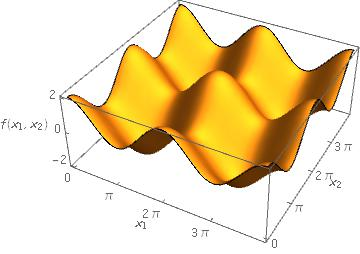
\includegraphics[width=0.5\textwidth,height=100pt]{mt1.jpg}

\end{figure}
\end{spacing}
\end{frame}
\begin{frame}[t]{3D Plots with Mathematica}
\begin{spacing}{1.2}
\includegraphics[scale=0.05]{mathematica.jpg}~\alert{2.2.1. Example.} The following Mathematica command creates the three-dimensional plot on the previous slide:
\begin{figure}
  \centering
  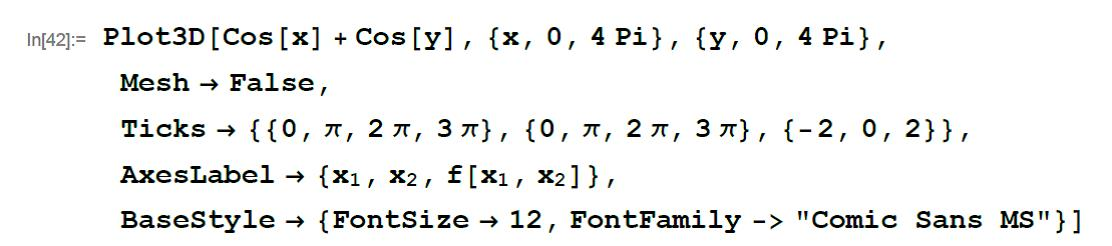
\includegraphics[width=\textwidth]{42.jpg}

\end{figure}
\end{spacing}
\end{frame}
\begin{frame}[t,allowdisplaybreaks,allowframebreaks]{Contour Plots}
\begin{spacing}{1}
Another representation for functions $f:\R^2\to\R$ is the so-called \emph{contour plot}. In this two-dimensional graph we plot curves
\[C_\alpha=f^{-1}(\{\alpha\})\]
for several values of $\alpha$. These are the pre-image sets (see (\eqref{2.1.11}) of $\{\alpha\}$.
\newpage
To illustrate, we successively show contours of
\[f:[0,4\pi]\times[0,4\pi]\to\R,\qquad\qquad f(x_1,x_2)=\cos x_1+\cos x_2\]
\begin{figure}
  \centering
  \includegraphics[width=0.5\textwidth,height=145pt]{mt2(2).jpg}

\end{figure}
\newpage
Instead of labeling, Mathematica can also color-code the contours
according to their values. Here, dark colors represent smaller values, light
colors larger values.
\begin{figure}
  \centering
  \includegraphics[scale=0.3]{mt3(2).jpg}

\end{figure}
\end{spacing}
\end{frame}
\begin{frame}[c]{Contour Plots with Mathematica}
\begin{spacing}{1.1}
\includegraphics[scale=0.05]{mathematica.jpg}~\alert{2.2.2. Example.} The following Mathematica commands creates the
contour plots on the previous slides:
\begin{figure}
  \centering
  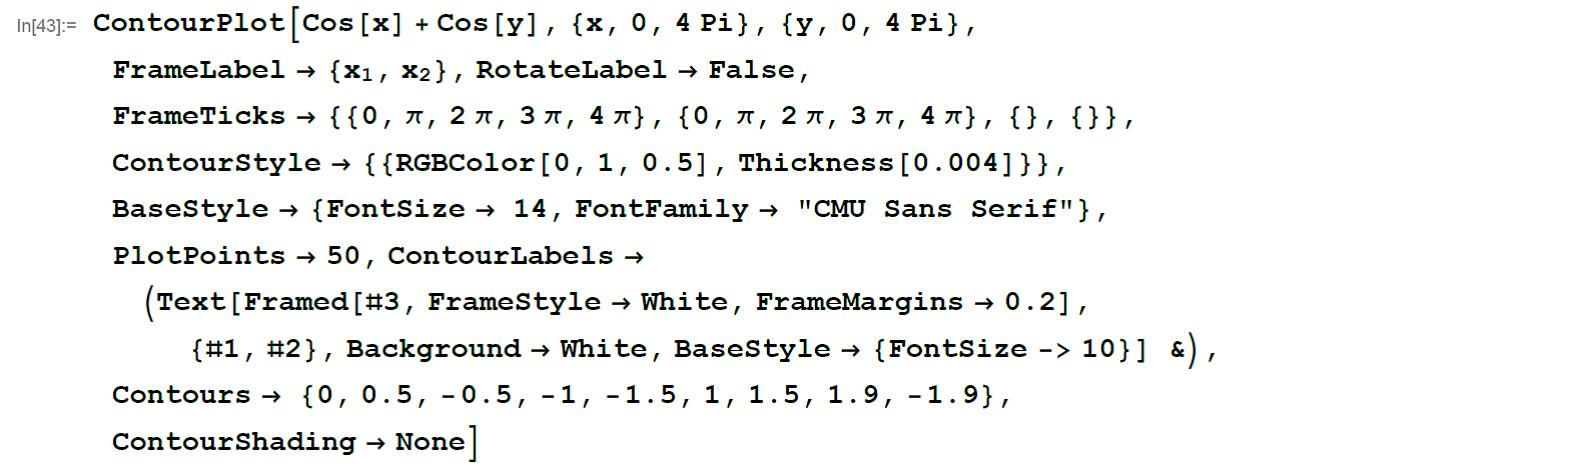
\includegraphics[width=\textwidth]{43.jpg}

\end{figure}
\begin{figure}
  \centering
  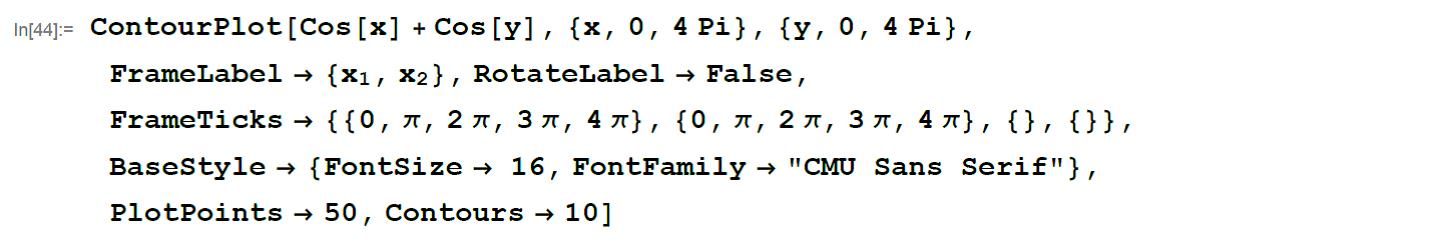
\includegraphics[width=\textwidth]{44.jpg}

\end{figure}
\end{spacing}
\end{frame}
\begin{frame}[t]{Contour Plots IV}
\begin{spacing}{1.05}
\alert{2.2.3. Example.} Sketch the contour plot of the function $f:\R^2\to\R,$\\$f(x,y)=x+y$.
\begin{figure}
  \centering
  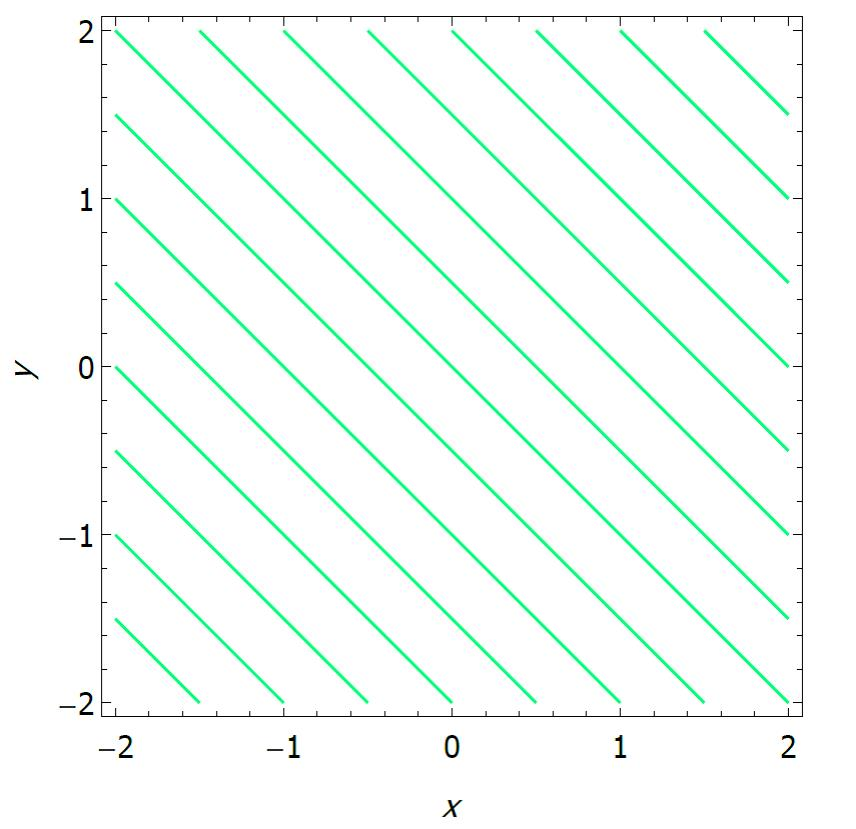
\includegraphics[width=0.55\textwidth,height=150pt]{mt4.jpg}

\end{figure}
\end{spacing}
\end{frame}
\begin{frame}[t,allowdisplaybreaks,allowframebreaks]{Phase Curves}
\begin{spacing}{1.05}
\vspace*{16pt}
In the hamiltonian formulation of analytical mechanics, one defines a
so-called \emph{Hamilton function} $H$ for a mechanical system. This function is
the sum of the kinetic energy ($T$) and potential energy ($V$). It represents
the total energy of the system, and remains constant if the system satisfies
the law of energy conservation (there are not, for example, any frictional
forces). We will assume this for our present discussion.\\[7pt]
In the hamiltonian formulation of mechanics, the essential variables of a
system are the position $x$ and the momentum $p$. The variables are tracked
in so-called \emph{phase space} $\R_{x}^{n}\times\R_{p}^{n}=\R_{(x,p)}^{2n}$, where, typically, $n=1,2$ or 3. The time-evolution of the system is represented through \emph{phase curves} in
$\R^{2n}$, which are given by the contour lines of H, which is regarded as a
function $\R^{2n}\to\R$. In other words, a phase curve is the set $H^{-1}(E)$, where
$E$ is the conserved energy of the system.
\newpage
\alert{2.2.4. Example.} For the simple harmonic oscillator, the kinetic energy is
given by $T=\frac{1}{2}mv^2=p^2/(2m)$ and the potential energy is given by $V=\frac{k}{2}x^2$, so
\[H(x,p)=\frac{1}{2m}p^2+\frac{k}{2}x^2.\]
\begin{columns}[c,onlytextwidth]
\begin{column}{0.6\textwidth}
The phase curves of the system are ellipses in $\R_{x,p}^2$, with each ellipse describing the behavior of a harmonic oscillator at a fixed energy $E$.
\end{column}
\begin{column}{0.4\textwidth}
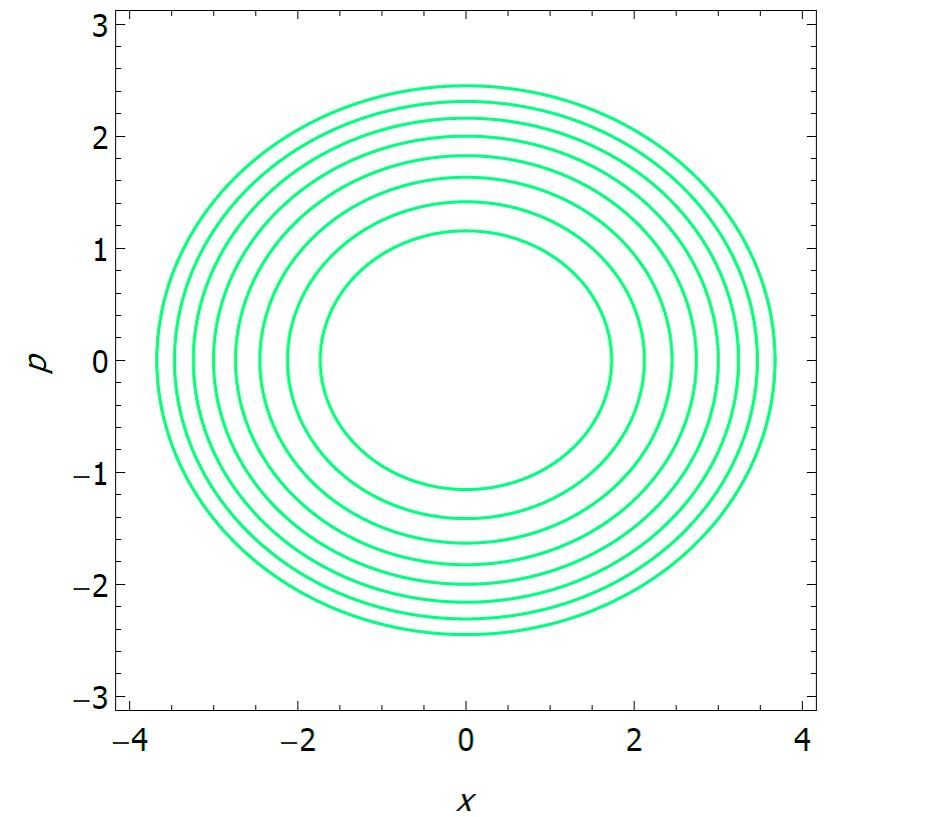
\includegraphics[width=\columnwidth]{mt5.jpg}
\end{column}
\end{columns}
\newpage
\alert{2.2.5. Example.} For a mathematical pendulum of length $l$ with mass $m$, $V=-mgl\cos\theta$, so
\[H(\theta,p)=\frac{1}{2m}p^2-mgl\cos\theta.\]
Sketch the phase curves of the pendulum for dif{}ferent energies and
interpret them physically!\\
\begin{center}
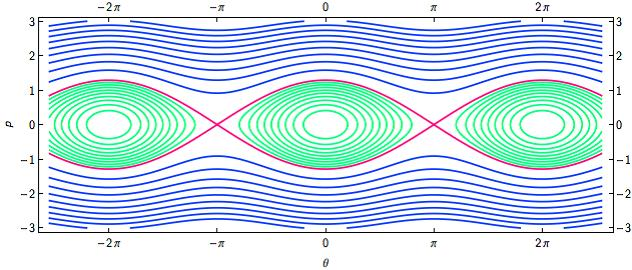
\includegraphics[width=0.8\textwidth]{mt6.jpg}
\end{center}
\end{spacing}
\end{frame}
\begin{frame}[t]{Calculus on Vector Spaces}
\begin{spacing}{1.1}
In the rest of this term we will develop calculus for "functions of multiple
variables". This generally means functions defined on (a subset of) $\R^n$, but
it is not any more dif{}ficult to treat functions defined on finite-dimensional
vector spaces.\\[6pt]
Throughout the following discussion, we assume that $V$ and $X$ denote
finite-dimensional, normed vector spaces. The concrete norm will be
irrelevant, as all norms are equivalent (see Theorem 2.1.11). We will
consider first the derivative of a function
\[f:X\to V.\]
\alert{2.2.6. Definition.} Let $f:X\to V_1,g:X\to V_2$ and $x_0\in X$. We say that
\[f(x)=o(g(x))\qquad\text{as}~x\to x_0\qquad\qquad\Leftrightarrow\qquad\qquad\lim_{x\to x_0}\frac{\|f(x)\|_{V_1}}{\|g(x)\|_{V_2}}=0\]
\end{spacing}
\end{frame}
\begin{frame}[t,allowdisplaybreaks,allowframebreaks]{The Derivative of a Function}
\begin{spacing}{0.95}
\alert{2.2.7. Definition.} Let $X,V$ be finite-dimensional vector spaces and $\Omega\subset X$ an open set. Then a map $f:\Omega\to V$ is called \emph{dif{}ferentiable at $x\in\Omega$} if there exists a linear map $L_x\in\mathcal{L}(X,V)$ such that
\setcounter{equation}{0}
\begin{equation}\label{2.2.1}
  f(x+h)=f(x)+L_xh+o(h)\qquad\qquad\text{as}~h\to 0.
\end{equation}
In this case we call $L_x$ the \emph{derivative of f at x} and write
\[L_x=Df|_x=df|_x.\]
We say that $f$ is dif{}ferentiable on $\Omega$ if it is dif{}ferentiable for every $x\in\Omega$.\\[5pt]
\alert{2.2.8. Remarks.}
\begin{itemize}
  \item Just as in the proof of 186 Lemma 3.1.2 we can show that the
derivative is uniquely defined by \eqref{2.2.1}.
  \item We may also copy the proof of Lemma 186 3.1.8 to see that every
dif{}ferentiable function is continuous.
\end{itemize}
\newpage
If $f$ is dif{}ferentiable on $\Omega$, we may regard $Df$ as a map
\[Df:\Omega\to\mathcal{L}(X,V),\qquad\qquad x\mapsto Df|_x.\]
\alert{2.2.9. Definition.} We define
\begin{align*}
  C(\Omega,V) &:=\{f:\Omega\to V:f~\text{is continuous}\}, \\
  C^1(\Omega,V) &:=\{f:\Omega\to V:f~\text{is dif{}ferentiable and $Df$ is continuous}\}.
\end{align*}
We may thus regard the \emph{derivative} $D$ as a (linear) map
\[D:C^1(\Omega,V)\to C(\Omega,\mathcal{L}(X,V)),\qquad\qquad f\mapsto Df.\]
\newpage
\alert{2.2.10. Example.} Let $X,V$ be finite-dimensional vector spaces and $L:\mathcal{L}(X,V)$ a linear map. Then
\[L(x+h)=Lx+Lh\xlongequal[]{!}Lx+DL|_xh+o(h)\qquad\quad(h\to0),\]
so the derivative of $L$ at any $x\in X$ is $DL|_x=L$.\\[12pt]
\alert{2.2.11. Examples.} Explicit instances of Example 2.2.10 are, e.g.,
\begin{itemize}
  \item Let $X=V=\C$ be regarded as real vector spaces and $f:z\to\overline{z}$ be the (then linear) complex conjugation. Then for $z,h\in\C$
      \[\overline{z+h}=\overline{z\mathstrut}+\overline{h\mathstrut},\]
      so $Df|_z(h)=\overline{h}$.
  \newpage
\vspace*{16pt}
  \item Regard $A\in\text{Mat}(2\times 2;\R)$ as a linear map $\R^2\to\R^2$. Then for $x,h\in\R^2$
      \[A(x+h)=Ax+Ah,\]
      so $DA|_x(h)=Ah$.
  \item Let tr:~$\text{Mat}(n\times n;\C)\to\C$ be the \emph{trace} of a square matrix, i.e.,
      \[\text{tr}\,A=\text{tr}(a_{ij})_{1\leq i,j\leq n}=\sum_{i=1}^{n}a_{ii}.\]
      Then the trace is linear and for $A,H\in\text{Mat}(n\times n;\C)$
      \[D\,\text{tr}|_AH=\text{tr}\,H.\]
\end{itemize}
\newpage
\alert{2.2.12. Example.} Some examples of derivatives of non-linear maps are as follows:
\begin{itemize}
  \item Let $X=V=\C$ be regarded as real vector spaces and $f:z\to z^2$. Then for $z,h\in\C$
      \[(z+h)^2=z^2+2zh+h^2,\]
      so $Df|_z(h)=2zh$.
  \item Let $f:\R^2\to\R$ be given by
  \[f(x)=f(x_1,x_2)=x_1+2x_2x_1+x_2^2.\]
  Then, for $h=(h_1,h_2)\in\R^2$ and $x\in\R^2$,
  \begin{equation*}
    \begin{split}
       f(x+h) &=f(x_1+h_1,x_2+h_2) \\
         &=x_1+h_1+2(x_2+h_2)(x_1+h_1)+(x_2+h_2)^2  \\
         &=f(x)+h_1+2(h_2x_1+h_1x_2+h_2x_2)+2h_1h_2+h_2^2.
    \end{split}
  \end{equation*}
\end{itemize}
\end{spacing}
\end{frame}
\begin{frame}[t,allowdisplaybreaks,allowframebreaks]{The Derivative of a Function as a Matrix}
\begin{spacing}{1}
In
\[f(x+h)=f(x)+\underbrace{h_1+2(h_2x_1+h_1x_2+h_2x_2)}_{=:L_{(x_1,x_2)}h}+2h_1h_2+h_2^2\]
the term $L_{(x_1,x_2)}h$ is clearly linear in $h$, while
\[\lim_{h\to0}\frac{\|2h_1h_2\|_{\R}}{\|h\|_{\R^2}}=\lim_{h_1,h_2\to0}\frac{|2h_1h_2|}{\sqrt{h_1^2+h_2^2}}=2\lim_{h_1,h_2\to0}\frac{|h_2|}{\sqrt{1+(h_2/h_1)^2}}.\]
Since $|h_2|\to0$ as $h_2\to0$ and $\nicefrac{1}{\sqrt{1+(h_2/h_1)^2}}$ is bounded, we see that
\[\lim_{h\to0}\frac{\|2h_1h_2\|_{\R}}{\|h\|_{\R^2}}=0,\]
and so $2h_1h_2=o(h)$ as $h\to0$. Similarly, we show that $h_2^2=o(h)$, so we conclude
\[Df|_xh=(1+2x_2)h_1+2(x_1+x_2)h_2.\]
\newpage
Notice that we may express the derivative as a $1\times 2$ matrix,
\begin{center}
$\displaystyle Df|_xh=\left(1+2x_2,2(x_1+x_2)\right)\binom{h_1}{h_2}.$
\end{center}
This is of course not surprising; if $X=\R^n$ and $V=\R^m$, i.e., we are considering a function
\[f:\R^n\supset\Omega\to\R^m,\qquad\quad f(x_1,\ldots,x_n)=\begin{pmatrix}
                    f_1(x_1,\ldots,x_n) \\
                    \vdots \\
                    f_m(x_1,\ldots,x_n)
                  \end{pmatrix},\]
then its derivative at $x\in\Omega$ (if it exists) is
\begin{center}
$Df|_x\in\mathcal{L}(\R^n,\R^m)\cong\text{Mat}(m\times n;\R).$
\end{center}
How to obtain this matrix? Denote by $e_j$ the $j$th standard basis vector in $\R^n$ or $\R^m$. We now consider the columns of $Df|_x$, which are given by $Df|_xe_j,$\\ $j=1,\ldots,n.$
\newpage
Assuming that $f$ is dif{}ferentiable, for any $h\in\R,x\in\R^n$ and $j=1,\ldots,n$ we have
\begin{center}
  $\displaystyle f(x+he_j)=f(x)+Df|_x(he_j)+o(h),$
\end{center}
which we may rewrite as
\[Df|_xe_j=\frac{1}{h}(f(x+he_j)-f(x))+o(1)
=\frac{1}{h}\sum_{k=1}^{m}(f_k(x+he_j)-f_k(x))e_k
+o(1).\]
The $(i,j)$th element of $Df|_x$ is given by $\scp{e_i}{Df|_xe_j}$, so
\[(Df|_x)_{ij}=\scp{e_i}{Df|_xe_j}=\frac{1}{h}
(f_i(x+he_j)-f_i(x))+o(1).\]
We now take the limit $h\to0$ to obtain
\[(Df|_x)_{ij}=\scp{e_i}{Df|_xe_j}=\lim_{h\to0}
\frac{f_i(x+he_j)-f_i(x)}{h}.\]
\end{spacing}
\end{frame}
\begin{frame}[t,allowdisplaybreaks,allowframebreaks]{Partial Derivatives}
\begin{spacing}{0.9}
\alert{2.2.13. Definition.} Let $\Omega\subset\R^n$ and $f:\Omega\to\R$ be dif{}ferentiable on $\Omega$.
We then define the \emph{partial derivative with
respect to $x_j$ at $x\in\Omega$} by
\begin{equation*}
  \begin{split}
     \left.\frac{\partial f}{\partial x_j}\right|_x &:=\lim_{h\to0}\frac{f(x+he_j)-f(x)}{h} \\
       &=\lim_{h\to0}\frac{f(x_1,\ldots,x_{j-1},x_j+h,x_{j+1},\ldots,x_n)-f(x)}{h}
  \end{split}
\end{equation*}
In this notation,
\begin{center}
  $\displaystyle(Df|_x)_{ij}=\frac{\partial f_i}{\partial x_j}$
\end{center}
or rather
\[Df|_x=\left.\begin{pmatrix}
          \frac{\partial f_1}{\partial x_1} & \cdots & \frac{\partial f_1}{\partial x_n} \\
          \vdots &  & \vdots \\
          \frac{\partial f_m}{\partial x_1} & \cdots & \frac{\partial f_m}{\partial x_n}
        \end{pmatrix}\right|_x\]
\newpage
There are several notations for he partial derivatives of a function. If $f:\R^n\to\R$, we may use any of the following:
\[\frac{\partial f}{\partial x_j}=\partial_{x_j}f=\partial_jf=f_{x_j}=f_j\]
to denote dif{}ferentiation w.r.t. the variable $x_j$. In practice, we calculate the partial derivative w.r.t. to $x_j$ by holding all other variables constant and simply dif{}ferentiating $f$ as a function of $x_j$.\\
\alert{2.2.14. Example.} Let $f(x_1,x_2,x_3)=x_1\sin(x_1x_2x_3)+3x_2^2x_1$. Then
\begin{align*}
  \frac{\partial f}{\partial x_1}&=\sin(x_1x_2x_3)+x_1x_2x_3\cos(x_1x_2x_3)+3x_2^2,\\
  \frac{\partial f}{\partial x_2}&=x_1^2x_3\cos(x_1x_2x_3)+6x_2x_1,\\
  \frac{\partial f}{\partial x_3}&=x_1^2x_2\cos(x_1x_2x_3).
\end{align*}
\end{spacing}
\end{frame}
\begin{frame}[c,allowdisplaybreaks,allowframebreaks]{The Jacobian}
\begin{spacing}{1}
Of course, if $Df|_x$ exists, we may write it as a matrix of partial derivatives.
However, it is not clear whether the existence of all partial derivatives
implies the existence of the derivative $Df|_x$. Thus it is useful to consider
the matrix of partial derivatives on its own; in fact, it deserves a special
designation.\\[6pt]
\alert{2.2.15. Definition.} Let $\Omega\subset\R^n$ and $f:\Omega\to\R^m$. Assume that all partial derivatives $\frac{\partial f_i}{\partial x_j}$ of $f$ exist at $x\in\Omega$. The matrix
\[J_f(x):=\left.\begin{pmatrix}
          \frac{\partial f_1}{\partial x_1} & \cdots & \frac{\partial f_1}{\partial x_n} \\
          \vdots &  & \vdots \\
          \frac{\partial f_m}{\partial x_1} & \cdots & \frac{\partial f_m}{\partial x_n}
        \end{pmatrix}\right|_x\]
called the \emph{Jacobian} of $f$.\\[4pt]
If the derivative $Df|_x\in\mathcal{L}(\R^n,\R^m)$ exists, $J_f(x)\in\text{Mat}(m\times n;\R)$ is the representing matrix of $Df|_x$ w.r.t. the standard bases in $\R^n$ and $\R^m$.
\newpage
\vspace*{11pt}
\alert{2.2.16. Example.} Let $f:\R^2\to\R^2$ be given by $f(x_1,x_2)=(x_1^2+x_2^2,x_2-x_1)$. Then the partial derivatives are
\begin{equation*}
  \begin{aligned}
  \frac{\partial f_1}{\partial x_1}&=\frac{\partial}{\partial x_1}(x_1^2+x_2^2)=2x_1,\\
  \frac{\partial f_2}{\partial x_1}&=\frac{\partial}{\partial x_1}(x_2-x_1)=-1,
  \end{aligned}
  \qquad\qquad
  \begin{aligned}
  \frac{\partial f_1}{\partial x_2}&=\frac{\partial}{\partial x_2}(x_1^2+x_2^2)=2x_2,\\
  \frac{\partial f_2}{\partial x_2}&=\frac{\partial}{\partial x_2}(x_2-x_1)=1.
  \end{aligned}
\end{equation*}
The Jacobian is given by
\[J_f(x_1,x_2)=\begin{pmatrix}
                 2x_1 & 2x_2 \\
                 -1 & 1
               \end{pmatrix}\]
The natural question that arises is,"Does the existence of $J_f(x)$ imply the dif{}ferentiability of $f$ and $x$?"
\newpage
\vspace*{3pt}
Regrettably, the answer to that question is negative, as the following
example shows:\\[6pt]
\alert{2.2.17. Examples.} Let $g:\R^2\to\R$ be given by
\[g(x_1,x_2)=\left\{\begin{aligned}
                      \frac{x_1x_2}{x_1^2+x_2^2}\qquad\quad(x_1,x_2)&\neq(0,0) \\
                      0\qquad\qquad\quad(x_1,x_2)&=(0,0)
                    \end{aligned}\right.\]
Then all partial derivatives of $g$ exist at $x=0$, since
\begin{equation*}
  \begin{aligned}
    \frac{\partial g}{\partial x_1}\Big|_{x=0}&=\lim_{h\to0}\frac{g(0+h,0)-g(0)}{h}=0,\\
    \frac{\partial g}{\partial x_2}\Big|_{x=0}&=\lim_{h\to0}\frac{g(0,0+h)-g(0)}{h}=0.
  \end{aligned}
\end{equation*}
Thus both partial derivatives exist at $x=0$ and in fact vanish.
\newpage
However, $g$ is not even continuous at $0$ since
\begin{equation*}
  \lim_{h\to0}g(h,h)=\frac{h^2}{h^2+h^2}=\frac{1}{2},\qquad\quad
  \lim_{h\to0}g(-h,h)=\frac{-h^2}{(-h)^2+h^2}=-\frac{1}{2}.
\end{equation*}
Thus $g$ can not be dif{}ferentiable at $x=0$.
\begin{figure}
  \centering
  \includegraphics[width=0.6\textwidth,height=130pt]{mt7(2).jpg}

\end{figure}
\newpage
\vspace*{6pt}
Thus the existence of the partial derivatives of a function $f:\R^n\to\R^m$ is not even enough to guarantee the continuity of $f$. However, we have the following result:\\[6pt]
\alert{2.2.18. Theorem.} Let $\Omega\subset\R^n$ be an open set and $f:\Omega\to\R^m$ such that all partial derivatives $\partial_{x_j}f_i$ exist on $\Omega$.
\begin{enumerate}[(i)]
  \item If all partial derivatives are bounded (there exists a constant $M>0$ such that $|\partial_{x_j}f_i|\leq M$ on $\Omega$), then $f$ is continuous i.e., $f\in C(\Omega,\R^m)$.
  \item If all partial derivatives are continuous on $\Omega$, then $f$ is continuously dif{}ferentiable on $\Omega$, i.e., $f\in C^1(\Omega,\R^m)$. In particular,
      \[Df|_x=J_f(x)=\left.\begin{pmatrix}
          \frac{\partial f_1}{\partial x_1} & \cdots & \frac{\partial f_1}{\partial x_n} \\
          \vdots &  & \vdots \\
          \frac{\partial f_m}{\partial x_1} & \cdots & \frac{\partial f_m}{\partial x_n}
        \end{pmatrix}\right|_x\]
      for all $x\in\Omega$.
\end{enumerate}
\newpage
\vspace*{17pt}
\alert{Proof.}\\
Let
\[f:\R^n\to\R^m,\qquad\qquad f(x)=\begin{pmatrix}
                                    f_1(x_1,\ldots,x_n) \\
                                    \vdots \\
                                    f_m(x_1,\ldots,x_n)
                                  \end{pmatrix}.\]
For both statements of the theorem, we need to consider $f(x+h)-f(x)$. To illustrate, let us first look at the case $n=2$. Then
\begin{equation*}
  \begin{split}
     f_i(x+h)-f_i(x) &=f_i(x_1+h_1,x_2+h_2)-f_i(x_1,x_2) \\
       &=[f_i(x_1+h_1,x_2+h_2)-f_i(x_1+h_1,x_2)]  \\
       &~~~~+[f_i(x_1+h_1,x_2)-f_i(x_1,x_2)].
  \end{split}
\end{equation*}
\newpage
\vspace*{14pt}
\alert{Proof (continued).}\\[5pt]
For fixed $h_1$, the first dif{}ference can be treated by the Mean Value Theorem 3.2.7 of Vv186: define
\[g:\R\to\R,\qquad\qquad\qquad g(y)=f_i(x_1+h_1,y).\]
Then there exists a $\theta_2\in(x_2,x_2+h_2)$ such that
\begin{equation*}
  \begin{split}
       &~~~f_i(x_1+h_1,x_2+h_2)-f_i(x_1+h_1,x_2) \\
       &=g(x_2+h_2)-g(x_2)  \\
       &=h_2\cdot g'(\theta_2)=h_2\partial_2f_i(x_1+h_1,x_2+\tau_2h_2)
  \end{split}
\end{equation*}
where we have chosen $\tau_2\in(0,1)$ such that $\theta_2=x_2+\tau_2h_2$.
\newpage
\alert{Proof (continued).}\\
Similarly, we find that
\[f_i(x_1+h_1,x_2)-f_i(x_1,x_2)=h_1\frac{\partial f_i}{\partial x_1}(x_1+\tau_1h_1,x_2)\]
for some $\tau_1\in(0,1)$. Generalizing to $n\geq2$, we have constants \myseries{\tau}{n}$\in(0,1)$ such that
\begin{equation*}
  \begin{split}
       &~~~~f_i(x+h)-f_i(x)  \\
       &=f_i(x_1+h_1,x_2+h_2,\ldots,x_n+h_n)-f_i(x_1,x_2+h_2,
       \ldots,x_n+h_n)  \\
       &~~~+f_i(x_1,x_2+h_2,\ldots,x_n+h_n)-f_i(x_1,x_2,x_3+h_3,\ldots,x_n+h_n)  \\
       &~~~+\cdots+f_i(x_1,x_2,\ldots,x_{n-1},x_n+h_n)-f_i(x_1,x_2,\ldots,x_n)  \\
       &=h_1\partial_1f_i(x_1+\tau_1h_1,x_2+h_2,\ldots,x_n+h_n)  \\
       &~~~+h_2\partial_2f_i(x_1,x_2+\tau_2h_2,x_3+h_3,\ldots,x_n+h_n)  \\
       &~~~+\cdots+h_n\partial_nf_i(x_1,x_2,\ldots,x_n+\tau_nh_n).
  \end{split}
\end{equation*}
\newpage
\alert{Proof (continued).}\\
We proceed with the proof of the theorem.
\begin{itemize}
  \item[(i)] Suppose that the partial derivatives are bounded. We want to prove that $f$ is continuous at $x\in\Omega$, i.e.,
      \[\lim_{h\to0}f(x+h)=f(x)\]
      where we are free to choose arbitrary norms in $\R^n$ and $\R^m$ for the convergence. In both spaces we choose the maximum norm $\|\cdot\|_{\infty}$ (see \eqref{2.1.4}):
  \begin{equation*}
    \begin{split}
       \|f(x+h)-f(x)\|_{\infty} &=\max_{i=1,\ldots,n}|f_i(x+h)-f_i(x)| \\
         &\leq n\cdot\max_{j=1,\ldots,n}|h_j|\max_{i,j=1,\ldots,n}\sup\limits_{x\to\Omega}\left|\frac{\partial f_i}{\partial x_j}(x)\right|  \\
         &\leq n\cdot M\cdot\|h\|_{\infty}\xrightarrow[]{h\to0}0.
    \end{split}
  \end{equation*}
\end{itemize}
\newpage
\alert{Proof (continued).}\\[7pt]
\begin{itemize}
  \item[(ii)] Write
  \[L=\left(\frac{\partial f_i}{\partial x_j}\right)_{\begin{subarray}
          ~i=1,\ldots,m\\
          j=1,\ldots,n
        \end{subarray}}=(L_{ij})_{\begin{subarray}
          ~i=1,\ldots,m\\
          j=1,\ldots,n
        \end{subarray}}\]
  for the Jacobian. We want to show that
  \[f(x+h)-f(x)-Lh=o(h)\qquad\qquad\text{as}~h\to0.\]
  We again choose the maximum norm $\|\cdot\|_{\infty}$ to establish the convergence and write
  \[u^j=(x_1,\ldots,x_{j-1},x_j+\tau_jh_j,x_{j+1}+h_{j+1},\ldots,x_n+h_n).\]
  for $j=1,\ldots,n$. We have the following estimate:
\end{itemize}
\newpage
\alert{Proof (continued).}
\begin{equation*}
  \begin{split}
     \|f(x+h)-f(x)-Lh\|_{\infty} &=\max_{i=1,\ldots,m}\Big|f_i(x+h)-f_i(x)-\sum_{j=1}^{n}L_{ij}h_j\Big| \\
       &=\max_{i=1,\ldots,m}\Big|\sum_{j=1}^{n}h_j(\partial_jf_i(u^j)-\partial_jf_i(x))\Big| \\
       &\leq\|h\|_{\infty}\sum_{j=1}^{n}\underbrace{\max_{i=1,\ldots,m}|\partial_jf_i(u^j)-\partial_jf_i(x)|}_{\to0~\text{as}~h\to0}  \\
       &=o(h)\qquad\quad\text{as}~h\to0.
  \end{split}
\end{equation*}
Observe that we use the assumption that $\partial_jf_i(x)$ is continuous at $x$. This proves that $f$ is dif{}ferentiable, $L=Df|_x$ and $Df|_x$ depends continuously on $x$.
\begin{flushright}
  $\square$
\end{flushright}
\newpage
\alert{2.2.19. Remark.} Let $\Omega\subset\R^n$ be an open set. Then
\begin{equation*}
  \begin{split}
     C^1(\Omega,\R^m) &:=\{f:\Omega\to\R^m:\partial_jf_i~\text{is continuous for}~j=1,\ldots,n \\
       &~~~\text{and}~i=1,\ldots,m\}.
  \end{split}
\end{equation*}
If $m=1$, we write $C^1(\Omega):=C^1(\Omega,\R)$ for short.\\[6pt]
We will next establish the product and chain rules for dif{}ferentiation.
\end{spacing}
\end{frame}
\begin{frame}[t]{Generalized Products}
 \begin{spacing}{1.05}
   To avoid having to re-prove the product rule for various types of products
that we will encounter, we first define a generalized product through
precisely those properties that we shall need.\\[6pt]
\alert{2.2.20. Definition.} Let $X_1,X_2,V$ be normed vector spaces. A map $\odot:X_1\times X_2\to V$ is called a \emph{(generalized) product} if
\begin{itemize}
  \item[1.] $\odot$ is bilinear, i.e., linear in each entry and
  \item[2.] $\|u\odot v\|_V\leq\|u\|_{X_1}\|v\|_{X_2}$ for all $u\in X_1,v\in X_2$.
\end{itemize}
\alert{2.2.21. Examples.}
\begin{itemize}
  \item[1.] The scalar products in $\R^n$ and $\C^n$;
  \item[2.] The cross product $\times:\R^3\times\R^3\to\R^3$;
  \item[3.] For a compact non-empty set $K\subset\R^n$ and $f,g\in C(K,\R)$ the pointwise product $f\cdot g\in C(K,\R)$, defined by
      \[(f\cdot g)(x)=f(x)g(x)\]
\end{itemize}
 \end{spacing}
\end{frame}
\begin{frame}[c,allowdisplaybreaks,allowframebreaks]{The Product Rule}
\begin{spacing}{0.9}
\vspace*{23pt}
\alert{2.2.22. Product Rule.} Let $U,X_1,X_2,V$ be finite-dimensional vector spaces and $\Omega\subset U$ an open set. Let $f:\Omega\to X_1$ and $g:\Omega\to X_2$ be dif{}ferentiable maps and $\odot:X_1\times X_2\to V$ a generalized product. Then $f\odot g:\Omega\to V$ is also dif{}ferentiable and
\begin{equation}\label{2.2.2}
  D(f\odot g)=(Df)\odot g+f\odot(Dg).
\end{equation}
At $x\in\Omega$ the right-hand side is interpreted as a linear map $U\to V$
\begin{equation}\label{2.2.3}
  u\mapsto D(f\odot g)|_xu=(Df|_xu)\odot g(x)+f(x)\odot(Dg|_xu).
\end{equation}
\newpage
\alert{Proof.}\\
The proof is similar to that for the product rule for functions of one
variable. We telescope the dif{}ference,
\begin{equation*}
  \begin{split}
       &~~f(x+h)\odot g(x+h)-f(x)\odot g(x)  \\
       &=f(x+h)\odot (g(x+h)-g(x))+(f(x+h)-f(x))\odot g(x)  \\
       &=(f(x)+O(h))\odot(Dg|_xh+o(h))+(Df|_xh+o(h))\odot g(x)
  \end{split}
\end{equation*}
as $h\to0$. Extending the relevant limit theorems from the pointwise
product to the generalized product, we have
\begin{equation*}
  \begin{split}
       &~~f(x+h)\odot g(x+h)-f(x)\odot g(x)  \\
       &=f(x)\odot (Dg|_xh)+O(\|h\|^2)+o(h)+(Df|_xh)\odot g(x)+o(h)  \\
       &=f(x)\odot(Dg|_xh)+(Df|_xh)\odot g(x)+o(h)
  \end{split}
\end{equation*}
\begin{flushright}
  $\square$
\end{flushright}
\end{spacing}
\end{frame}
\begin{frame}[t,allowdisplaybreaks,allowframebreaks]{The Chain Rule}
\begin{spacing}{1}
\alert{2.2.23. Chain Rule.} Let $U,X,V$ be finite-dimensional vector spaces and $\Omega\subset U,\Sigma\subset X$ open sets. Let $g:\Omega\to\Sigma$ and $f:\Sigma\to V$ be dif{}ferentiable maps. Then the composition $f\circ g:\Omega\to V$ is also dif{}ferentiable and for all $x\in\Omega$
\begin{equation}\label{2.2.4}
  D(f\circ g)|_x=Df|_{g(x)}\circ Dg|_x,
\end{equation}
where the right-hand side is a composition of linear maps.\\[5pt]
The proof is basically identical to that of 186 Theorem 3.1.12, the chain
rule for functions of one real variable. You are encouraged to revisit that
proof and apply it to the general chain rule here.\\[4pt]
\alert{2.2.24. Example.} Consider the polar coordinates $(r,\phi)\in(0,\infty)\times[0,2\pi),$ defined through the map
\[\Phi(r,\phi)=\binom{r\cos\phi}{r\sin\phi}.\]
\newpage
Then
\[D\Phi|_{(r,\phi)}=\begin{pmatrix}
                      \frac{\partial\Phi_1}{\partial r} & \frac{\partial\Phi_1}{\partial \phi} \\
                      \frac{\partial\Phi_2}{\partial r} & \frac{\partial\Phi_2}{\partial \phi}
                    \end{pmatrix}=\begin{pmatrix}
                                    \cos\phi & -r\sin\phi \\
                                    \sin\phi & r\cos\phi
                                  \end{pmatrix}.\]
Next, consider the map $U:\R^2\to\R,(x_1,x_2)\mapsto x_1^2+x_2^2$. The derivative is
\[DU|_x=\left(\frac{\partial U}{\partial x_1},\frac{\partial U}{\partial x_2}\right)=(2x_1,2x_2)\]
Now $U\circ\Phi=(r\cos\phi)^2+(r\sin\phi)^2=r^2$. Clearly, $D(U\circ\Phi)|_{(r,\phi)}=(2r,0)$. We can also apply the chain rule
\begin{equation*}
  \begin{split}
     D(U\circ\Phi)|_{(r,\phi)} &=DU|_{(r\cos\phi,r\sin\phi)}D\Phi|_{(r,\phi)} \\
       &=(2r\cos\phi,2r\sin\phi)\begin{pmatrix}
                                  \cos\phi & -r\sin\phi \\
                                  \sin\phi & r\cos\phi
                                \end{pmatrix} \\
       &=(2r\cos^2\phi+2r\sin^2\phi,-2r^2\cos\phi\sin\phi+2r^2\sin\phi\cos\phi)  \\
       &=(2r,0)
  \end{split}
\end{equation*}
\end{spacing}
\end{frame}
\begin{frame}[t]{Integrals of Vector-Space-Valued Functions}
\begin{spacing}{1}
The following important result will require the integral of a function of a
single variable, albeit with values in a vector space $V$. In other words, we
need to assign a meaning to
\[\int_{a}^{b}f(x)dx,\qquad\qquad\text{where}~f:[a,b]\to V.\]
Fortunately, the procedure is completely analogous to that of functions $f:\R\to\R$, at least for the regulated integral: we define step functions on $[a,b]$ with respect to a partition $\mathcal{P}$ by setting them constant on sub-intervals of the partition:\\[14pt]
\alert{2.2.25. Definition.} A $V$ be a real or complex vector space. A function $f:[a,b]\to V$ is called a \emph{step function with respect to a partition $P=(a_0,\ldots,a_n)$} if there exist elements $y_i\in V$ such that $f(t)=y_i$ whenever $a_{i-1}<t<a_i$,\\$i=1,\ldots,n$. We denote the set of all step functions by Step$([a,b],V)$
\end{spacing}
\end{frame}
\begin{frame}[t]{Step Functions}
\begin{spacing}{1}
\alert{2.2.26. Example.} The map
\begin{equation*}
  f:[0,1]\to\R^2,\qquad\qquad f(x)=\left\{\begin{subarray}
  ~\binom{0}{1/2}\qquad 0\leq x<1/2\\
  \binom{1}{1}\qquad ~~x=1/2\\
  \binom{2}{0}\qquad ~~1/2<x\leq 1
            \end{subarray}\right.
\end{equation*}
is a step function.\\[5pt]
We then follow through with analogous definitions to the ones for real
functions, replacing the modulus in $\R$ by the norm in a vector space:\\[5pt]
\alert{2.2.27. Definition.} Let $I\subset\R$ be an interval and $(V,\|\cdot\|_V)$ a normed vector space. We say that a map $f:I\to V$ is \emph{bounded} if
\begin{equation}\label{2.2.5}
  \|f\|_{\infty}:=\sup\limits_{x\in I}\|f(x)\|_V<\infty.
\end{equation}
The set of all bounded functions $f:I\to V$ is denoted $L^{\infty}(I,V)$.
\end{spacing}
\end{frame}
\begin{frame}[c]{Bounded Functions}
\begin{spacing}{1.05}
\alert{2.2.28. Example.} The map
\[f:\R\to\R^2,\qquad\qquad\qquad f(t)=\binom{\sin t}{e^{-t^2}}\]
is a bounded map. To see this, we endow $\R^2$ with the norm $\|x\|_1:=|x_1|+|x_2|$. (Since all norms inn $\R^n$ are equivalent, it doesn't matter which norm we take.) Then
\begin{equation*}
  \begin{split}
     \|f\|_{\infty} &:=\sup\limits_{t\in\R}\|f(t)\|_1=\sup\limits_{t\in\R}(|\sin t|+|e^{-t^2}|) \\
       &\leq\sup\limits_{t\in\R}|\sin t|+\sup\limits_{t\in\R}|e^{-t^2}|=2<\infty.
  \end{split}
\end{equation*}
\end{spacing}
\end{frame}
\begin{frame}[c,allowdisplaybreaks,allowframebreaks]{Integrals of Step Functions}
\begin{spacing}{1.05}
\vspace*{16pt}
We then define the integral of a step function as before:\\[6pt]
\alert{2.2.29. Theorem.} Let $f:[a,b]\to V$ be a step function with respect to some partition $P$. Then
\[I_p(f):=(a_1-a_0)y_1+\cdots+(a_n-a_{n-1})y_n\in V\]
is independent of the choice of the partition $P$ and is called the \emph{integral} of $f$.\\[5pt]
Note that if $f:[a,b]\to V$, then $\int_{a}^{b}f(x)dx\in V$, the integral of $f$ is an element of the space $V$.\\[6pt]
(This makes it impossible to define the Riemann integral for functions $f:I\to V$, because it relies comparing the size of upper and lower step functions.)
\newpage
\vspace*{19pt}
The main ingredient is again uniform convergence, where we now say that a sequence of functions $(f_n),f_n:I\to V,I\subset\R$, converges uniformly to $f:I\to V$ in a normed vector space $(V,\|\cdot\|_V)$ if
\[\|f_n-f\|_{\infty}:=\sup_{x\in I}\|f_n(x)-f(x)\|_V\xrightarrow[]{x\to\infty}0.\]
The set of regulated functions is then the closure of the set of step
functions in the uniform norm. You are invited to check that everything in
fact works just as in the regulated integral for scalar real functions!
\newpage
The upshot is the following: if $f:[a,b]\to\R^n$ is piecewise continuous, then $f$ is regulated and
\[\int_{a}^{b}f(x)dx=\int_{a}^{b}\begin{pmatrix}
                                   f_1(x) \\
                                   \vdots \\
                                   f_n(x)
                                 \end{pmatrix}dx=\begin{pmatrix}
                                                   \int_{a}^{b}f_1(x)dx \\
                                                   \vdots \\
                                                   \int_{a}^{b}f_n(x)dx
                                                 \end{pmatrix}\]
(This follows because a sequence of step functions converging uniformly to
f will converge uniformly in each component; the individual components
are then equal to the "usual" regulated integrals of real-valued functions.)\\[5pt]
Furthermore, we have the standard estimate
\[\left|\int_{a}^{b}f(x)dx\right|_V\leq\int_{a}^{b}\|f(x)\|_Vdx\leq|b-a|\cdot\sup\limits_{x\in[a,b]}\|f(x)\|_V.\]
\end{spacing}
\end{frame}
\begin{frame}[c,allowdisplaybreaks,allowframebreaks]{The Mean Value Theorem}
\begin{spacing}{1.05}
In general, the mean value theorem (186 Theorem 3.2.7) that we proved
last term does not survive here. However, we can formulate an "integrated
version:"\\[5pt]
\alert{2.2.30. Mean Value Theorem.} Let $X,V$ be finite-dimensional vector spaces, $\Omega\subset X$ open and $f\in C^1(\Omega,V)$. Let $x,y\in\Omega$ and assume that the line segment $x+ty,0\leq t\leq 1$, is wholly contained in $\Omega$. Then
\begin{equation}\label{2.2.6}
  f(x+y)-f(x)=\int_{0}^{1}Df|_{x+ty}ydt=\left(\int_{0}^{1}Df|_{x+ty}dt\right)y.
\end{equation}
\alert{2.2.31. Remark.} The integrals in \eqref{2.2.6} are integrals of elements of $V$ (the integrand $Df|_{x+ty}y$) and $\mathcal{L}(X,V)$~(the integrand $Df|_{x+ty}$). The definition of the regulated integral in Vv186 can easily be extended to such vector-space valued functions. However, in the case of $V=\R^m$ and $\mathcal{L}(X,V)=\text{Mat}(m\times n;\R)$ the vectors and matrices are simply integrated in each component to yield again vectors and matrices, respectively.
\newpage
The Mean Value Theorem 2.2.30 can also be understood as a
generalization of the fundamental theorem of calculus: For single-variable
functions, the fundamental theorem of calculus can be expressed as
\[f(x+y)-f(x)=\int_{x}^{x+y}f'(\xi)d\xi.\]
Substituting $t=(\xi-x)/y$ in the integral, we have the equivalent identity
\[f(x+y)-f(x)=\int_{0}^{1}f'(x+yt)ydt,\]
a special case of \eqref{2.2.6}.
\newpage
\alert{Proof of Theorem 2.2.30.}\\
Define the auxiliary function $g\in C^1([0,1],V)$ by $g(t):=f(x+ty)$. Thus (by 186 Lemma 4.2.3) we have
\[f(x+y)-f(x)=g(1)-g(0)=\int_{0}^{1}g'(t)dt.\]
For $\gamma(t)=x+ty$ we have $\gamma'(t)=y$. Applying the chain rule,
\[g'(t)=D(f\circ\gamma)|_t=Df|_{\gamma(t)}D\gamma|_t=Df|_{x+ty}y.\]
Thus we obtain
\[f(x+y)-f(x)=\int_{0}^{1}Df|_{x+ty}ydt.\]
proving the first equality.
\newpage
\alert{Proof of Theorem 2.2.30 (continued).}\\
We now prove that $y$ may be "taken out" of the integral. Let us abbreviate $L(t)=Df|_{x+ty}$. For $z\in(0,1)$ we have
\[\frac{d}{dz}\int_{0}^{z}L(t)ydt=L(z)y=\frac{d}{dz}\left\{\left(\int_{0}^{z}
L(t)dt\right)y\right\}.\]
Furthermore, setting $z=0$ we have
\[\int_{0}^{0}L(t)ydt=0=\left(\int_{0}^{0}L(t)dt\right)y.\]
Therefore,
\[\int_{0}^{z}L(t)ydt=\left(\int_{0}^{z}L(t)dt\right)y\]
for all $z\in[0,1]$, in particular also for $z=1$.\multido{}{7}{\qquad}\quad{$\square$}
\newpage
\alert{2.2.32. Corollary.} From the standard estimate
\[\bigg\|\int_{a}^{b}f(t)dt\bigg\|_V\leq|b-a|\cdot\sup_{t\in[a,b]}\|f(t)\|_V\]
Theorem 2.2.30 yields
\[\|f(x+y)-f(x)\|_V\leq\|y\|_X\cdot\sup_{0\leq t\leq 1}\|Df|_{x+ty}\|,\]
where $\|Df|_{x+ty}\|$ denotes the operator norm of $Df|_{x+ty}\in\mathcal{L}(X,V)$.
\end{spacing}
\end{frame}
\begin{frame}[t,allowdisplaybreaks,allowframebreaks]{Dif{}ferentiating
Under an Integral}
\begin{spacing}{1.05}
We close this section with a useful result concerning the interchanging of
dif{}ferentiation and integration.\\[6pt]
\alert{2.2.33. Theorem.} Let $X,V$ be finite-dimensional vector spaces, $I=[a,b]\subset\R$ an interval and $\Omega\subset X$ an open set. Let $f:I\times\Omega\to V$ be a continuous function such that $Df(t,\cdot)$ exists and is continuous for every $t\in I$. Then
\[g(x)=\int_{a}^{b}f(t,x)dt\]
is dif{}ferentiable in $\Omega$ and
\[Dg(x)=\int_{a}^{b}Df(t,\cdot)|_xdt\]
\newpage
\alert{Proof.}\\
Fix $x\in\Omega$ and choose $h$ small enough such that $x+h\in\Omega$. In any case, we assume $\|h\|<1$. We need to prove
\begin{equation}\label{2.2.7}
  g(x+h)-g(x)-\underbrace{\left(\int_{a}^{b}Df(t,\cdot)|_xdt
  \right)}_{=:L}h=o(h).
\end{equation}
By the Mean Value Theorem, the left-hand side equals
\begin{equation*}
  \begin{split}
       &~~~\int_{a}^{b}\left(f(t,x+h)-f(t,x)-Df(t,\cdot)|_xh\right)dt  \\
       &=\int_{a}^{b}\left(\int_{0}^{1}Df(t,\cdot)|_{x+sh}ds\,h-Df(t,\cdot)|_xh\right)dt \\
       &=\int_{a}^{b}\left(\int_{0}^{1}\left(Df(t,\cdot)|_{x+sh}-Df(t,\cdot)|_x\right)\,ds\right)hdt.
  \end{split}
\end{equation*}
\newpage
\alert{Proof (continued).}\\
Taking the norm, we have
\begin{equation*}
  \begin{split}
       &~~~\|g(x+h)-g(x)-Lh\|_V  \\
       &\leq(b-a)\sup\limits_{t\in[a,b]}\bigg\|\int_{0}^{1}\left(Df(t,\cdot)|_{x+sh}-Df(t,\cdot)|_x\right)ds\bigg\|\cdot\|h\|_X  \\
       &\leq(b-a)\sup\limits_{t\in[a,b]}\sup\limits_{s\in[0,1]}\left\|Df(t,\cdot)|_{x+sh}-Df(t,\cdot)|_x\right\|\cdot\|h\|_X
  \end{split}
\end{equation*}
Here $\|\cdot\|$ denotes the operator norm. We now need to show that
\[\sup_{t\in[a,b]}\sup_{s\in[0,1]}\left\|Df(t,\cdot)|_{x+sh}-Df(t,\cdot)|_x\right\|\]
vanishes when $h\to0$. However, this requires a subtle argument, because $s$ and $t$ are free to vary independent of $h$.
\newpage
\alert{Proof (continued).}\\
Consider the function $Df(t,\cdot)|_y$ where $y$ varies in the closed and bounded set $\overline{B_1(x)}$. Since $V$ is finite-dimensional, this set is compact and so is $[a,b]\times\overline{B_1(x)}$.\\[5pt]
Since $Df(t,\cdot)|_y$ is continuous in the compact set $[a,b]\times\overline{B_1(x)}$, it is also uniformly continuous by Theorem 2.1.38. Hence, if $\varepsilon>0$ is given we can find $\delta>0$ such that
\[\|h\|_X<\delta\qquad\quad\Rightarrow\qquad\quad\big\|Df(t,
\cdot)|_{x+sh}-Df(t,\cdot)|_x\big\|<\varepsilon,\]
independent of $s$ and $t$. This implies that
\[\|h\|_X<\delta\qquad\Rightarrow\qquad\frac{\|g(x+h)-g(x)-Lh\|_V}{\|h\|_X}
<(b-a)\varepsilon,\]
proving \eqref{2.2.7}.
\newpage
\vspace*{17pt}
Dif{}ferentiating an integral with respect to a parameter can be very useful
for calculating integrals that are otherwise dif{}ficult to evaluate directly. For
example, by dif{}ferentiating
\[g(x):=\int_{0}^{\infty}\frac{\sin t}{t}e^{-xt}dt\]
with respect to $x$ you will show in the assignments that
\[g(0)=\int_{0}^{\infty}\frac{\sin t}{t}dt=\frac{\pi}{2}.\]
(Compare with the discussion of the Dirichlet integral last term, see
186 Example 4.2.14.)
\end{spacing}
\end{frame}
\subsection{Curves in Vector Spaces}
\begin{frame}[c]
\begin{spacing}{2.5}
\tableofcontents[sectionstyle=hide,subsectionstyle=show/shaded/hide]
\end{spacing}
\end{frame}
\begin{frame}[t]{Curves}
\begin{spacing}{1}
An important case of a map between vector space is a map $\R\to V$, where $(V,\|\cdot\|)$ is a normed vector space.\\[4pt]
\alert{2.3.1. Definition.} Let $V$ be a finite-dimensional vector space and $I\subset\R$ an interval.
\begin{itemize}
  \item A set $\mathcal{C}\subset V$ for which there exists a continuous, surjective and locally injective map $\gamma:I\to\mathcal{C}$ is called a \emph{curve}.
  \item The map $\gamma$ is called a \emph{parametrization} of $\mathcal{C}$.
  \item A curve $\mathcal{C}$ together with a parametrization is called a \emph{parametrized} curve.
\end{itemize}
\vspace*{12pt}
\alert{2.3.2. Remark.} Here \emph{locally injective} means that in the neighborhood $B_{\varepsilon}(x)\cap I$ of any point $x\in I$ the parametrization is injective.\\[5pt]
More generally, let f be a function of a single real variable. We say that a
property holds \emph{locally at a point} $p\in\R$ if this property holds in some $\varepsilon$-neighborhood $B_{\varepsilon}(p)$.
\end{spacing}
\end{frame}
\begin{frame}[c]{Local Properties of Real Functions}
\begin{spacing}{1.1}
\alert{2.3.3. Examples.}
\begin{itemize}
  \item If $f\in C(\R)$ and $f(0)>0$, then $f$ is \emph{locally positive at} 0.
  \item If $f\in C^1(\R)$ and $f'(0)>0$, then $f$ is \emph{locally increasing at} 0.
  \item If $f\in C^1(\R)$ and $f'(0)\neq0$, then $f$ is \emph{locally invertible at} 0.
\end{itemize}
We simply say that a property holds locally if this property holds locally at
every point $p\in\R$.\\[5pt]
\alert{2.3.4. Example.} The sequence of functions $(f_n)$ given by $f_n(x)=(x-1/n)^2$ converges to $f(x)=x^2$ locally uniformly, because at every point $p\in\R$ there is an $\varepsilon$-neighborhood such that the convergence is uniform in this neighborhood.
\end{spacing}
\end{frame}
\begin{frame}[t,allowdisplaybreaks,allowframebreaks]{Curves}
\begin{spacing}{0.9}
\alert{2.3.5. Example.} The set
\[S^1:=\{(x_1,x_2)\in\R^2:x_1^2+x_2^2=1\}\]
is a curve in $\R^2$ because we can find a parametrization, e.g.,
\[\gamma:[0,2\pi]\to S^1,\qquad\qquad\qquad\quad\gamma(t)=\binom{\cos(t)}{\sin(t)}.\]
It is clear that $\gamma$ is continuous. Furthermore, $\text{ran}\,\gamma\subset S^1$ since
\[\cos^2 t+\sin^2 t=1\qquad\qquad\qquad\text{for all}\,t\in[0,2\pi].\]
The map $\gamma$ is not injective, since $\gamma(0)=\gamma(2\pi)=(1,0)$, but it is injective on $(0,2\pi)$: If $\gamma(t_1)=\gamma(t_2)\neq(1,0)$, then $\cos t_1=\cos t_2$ and $\sin t_1=\sin t_2$. The second equation implies $t_1,t_2\in(0,\pi]$ or $t_1,t_2\in(\pi,2\pi)$. However, since the cosine function is injective on $(0,\pi]$ and on $(\pi,2\pi)$ we obtain $t_1=t_2$. Hence\\ $\gamma$ is locally injective.
\newpage
Now suppose $(x_1,x_2)\in S^1$ is given. Then taking
\setcounter{equation}{0}
\begin{equation}\label{2.3.1}
  t_0=\left\{\begin{array}{ll}
                 \arctan\frac{x_2}{x_1} & \text{if}\,x_2>0,x_1\neq0,\\[4pt]
                 \pi/2 & \text{if}\,(x_1,x_2)=(0,1), \\[4pt]
                 \pi+\arctan\frac{x_2}{x_1} & \text{if}\,x_2<0,x_1\neq0, \\[4pt]
                 3\pi/2 & \text{if}\,(x_1,x_2)=(0,-1), \\[4pt]
               \end{array}\right.
\end{equation}
(where we use a suitable branch of the inverse tangent) gives $\gamma(t_0)=(x_1,x_2)$ for some $t_0\in[0,2\pi]$. Thus, $\gamma$ is surjective and therefore a parametrization.\\[6pt]
Another parametrization is
\[\widetilde{\gamma}:[0,1]\to S^1,\qquad\qquad\quad\widetilde{\gamma}(t)=\binom{\cos(2\pi t)}{-\sin(2\pi t)}.\]
Both $(\mathcal{C},\gamma)$ and $(\mathcal{C},\widetilde{\gamma})$ are parametrized curves.
\end{spacing}
\end{frame}
\newpage
\begin{frame}[c]{Parametrizations of Curves}
\begin{spacing}{1}
It is clear that a curve will have an infinite number of parametrizations.
Physically, a curve $\mathcal{C}$ might be considered to be the path of a particle, while
the parametrization $\gamma$ gives the position of the particle at each time $t$.\\[9pt]
Hence, in Example 2.3.5, $\gamma$ describes the counter-clockwise movement of a particle around the unit circle, while $\widetilde{\gamma}$ describes a clockwise movement around the same path. The parametrization $\gamma$ corresponds to completing the path in time $2\pi$, while $\widetilde{\gamma}$ corresponds to completing the path in time 1. Hence, the parametrization $\widetilde{\gamma}$ can be said to correspond to a greater velocity of the particle.
\end{spacing}
\end{frame}
\begin{frame}[t]{Simple, Open and Closed Curves}
\begin{spacing}{1}
\alert{2.3.6. Definition.} Let $\mathcal{C}\subset V$ be a curve possessing a parametrization $\gamma:I\to\mathcal{C}$ with $\text{int}\,I=(a,b)$ for $-\infty\leq a<b\leq\infty$.
\begin{itemize}
  \item[(i)] If $\gamma$ is (globally) injective parametrization we say that $\mathcal{C}$ is a \emph{simple curve}.
  \item[(ii)] If
  \[\lim_{t\to a}\gamma(t)=\lim_{t\to b}\gamma(t),\]
  the curve $\mathcal{C}$ is said to be \emph{closed}.
  \item[(iii)] If a curve is not closed, it is said to be \emph{open}. The points
      \[x:=\lim_{t\to a}\gamma(t)\qquad\qquad\text{and}\qquad\qquad y:=\lim_{t\to b}\gamma(t)\]
      are called the \emph{initial point} and the \emph{final point} of the parametrized curve $(\mathcal{C},\gamma)$. The open curve is said t join $x$ and $y$.
\end{itemize}
\end{spacing}
\end{frame}
\begin{frame}[t]{Sketches of Simple, Open and Closed Curves}
\vspace*{-20pt}
\begin{figure}
  \centering
  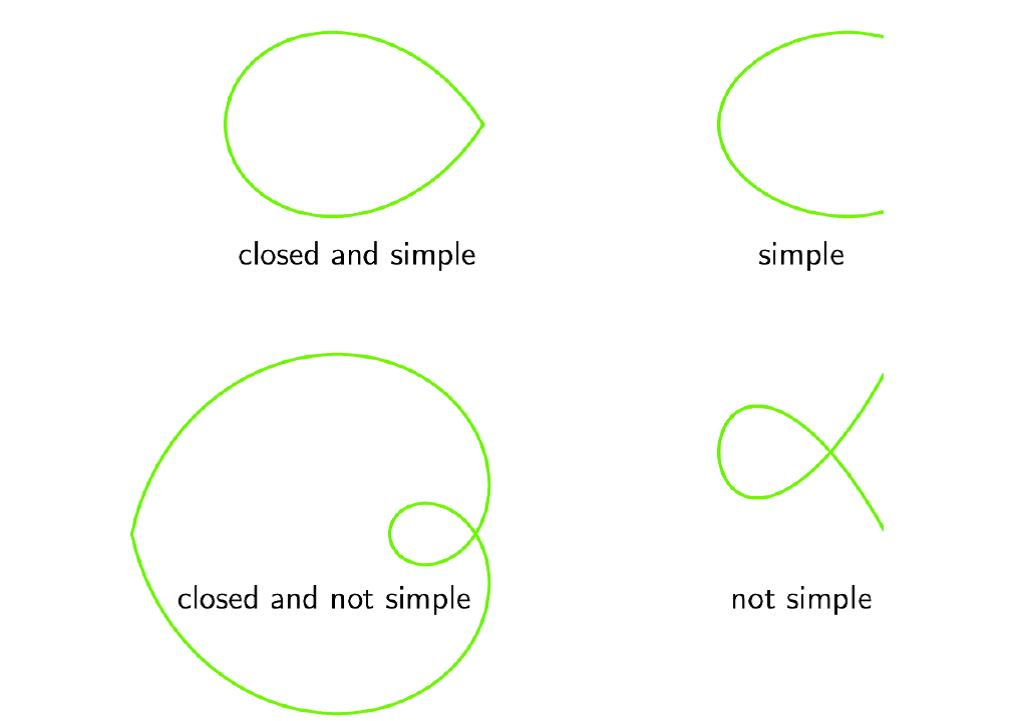
\includegraphics[width=\textwidth,height=200pt]{curves.jpg}

\end{figure}
\end{frame}
\begin{frame}[c]{Initial and Final Points of Open Curves}
\begin{spacing}{1}
\alert{2.3.7. Remark.} Whether a point is an initial or final point of an open curve
depends on the parametrization. We will explore this a little further.\\[5pt]
\alert{2.3.8. Example.} The simple open curve
\[\mathcal{C}=\{(x_1,x_2)\in\R^2:0\leq x_1\leq 1,x_2=x_1^2\}\]
joins the points $x=(0,0)$ and $y=(1,1)$. Either may be considered the initial point or the final point. Possible parametrizations are
\[\gamma(t)=\binom{t}{t^2},\qquad\qquad\qquad\widetilde{\gamma}
(t)=\binom{1-t}{(1-t)^2}\]
where both $\gamma,\widetilde{\gamma}:[0,1]\to \mathcal{C}.$
\end{spacing}
\end{frame}
\begin{frame}[t,allowdisplaybreaks,allowframebreaks]{Reparametrization of Curves}
\begin{spacing}{1.1}
\alert{2.3.9. Definition.} Let $\mathcal{C}\subset V$ be a curve with parametrization $\gamma:I\to\mathcal{C}$.
\begin{itemize}
  \item[(i)] Let $J\subset\R$ be an interval. A continuous, bijective map $r:J\to I$ is called a \emph{reparametrization} of the parametrized curve $(\mathcal{C},\gamma)$.
  \item[(ii)] If $r$ is \emph{increasing} the reparametrization is said to be \emph{orientation-preserving}.
  \item[(iii)] If $r$ is \emph{decreasing} the reparametrization is said to be \emph{orientation-reversing}.
\end{itemize}
\vspace*{12pt}
\alert{2.3.10. Remarks.}\\
\begin{enumerate}[(i)]
  \item Given any two parametrizations $\gamma,\widetilde{\gamma}$ of an open curve, one can always find a reparametrization by setting $r=\gamma^{-1}\circ\widetilde{\gamma}$(the
      continuity and local injectivity is enough for this definition to make sense).
  \item Since every bijective map in $\R$ is either decreasing or increasing (see 186 Theorem 2.5.20), it follows that a reparametrization is either orientation-preserving or orientation-reversing.
\end{enumerate}
\newpage
\alert{2.3.11. Example.} Consider the unit circle $S^1$ of Example 2.3.5 with parametrizations
\begin{center}
  $\displaystyle\gamma:[0,2\pi]\to S^1,\qquad\qquad\quad\gamma(t)=\binom{\cos(t)}{\sin(t)},$\\[6pt]
  $\displaystyle\widetilde{\gamma}:[0,1]\to S^1,\qquad\qquad\quad\widetilde{\gamma}(t)=\binom{\cos(2\pi t)}{-\sin(2\pi t)}$.
\end{center}
Then $r:[0,1]\to[0,2\pi],\,r(t)=-2\pi t$, is a reparametrization of the parametrized curve $(\mathcal{C},\gamma)$. In fact,
\[\widetilde{\gamma}=\gamma\circ r.\]
The reparametrization is not orientation-preserving since $r'(t)=-2\pi<0$.
\end{spacing}
\end{frame}
\begin{frame}[c,allowdisplaybreaks,allowframebreaks]{Orientation of Curves}
\begin{spacing}{1.05}
A reparametrization of a parametrized curve $(\mathcal{C},\gamma)$ yields a new parametrized curve $(\mathcal{C},\widetilde{\gamma})$ where $\widetilde{\gamma}=\gamma\circ r$.\\[5pt]
It is easy to see that an orientation-preserving reparametrization of an
open curve $(\mathcal{C},\gamma)$ yields an open parametrized curve $(\mathcal{C},\widetilde{\gamma})$ with the same initial and final points.\\[6pt]
\alert{2.3.12. Definition.} Let $(\mathcal{C},\gamma)$ be a parametrized curve and $r$ a reparametrization of $(\mathcal{C},\gamma)$.\\[4pt]
The curve $(\mathcal{C},\widetilde{\gamma})$ with $\widetilde{\gamma}=\gamma\circ r$ is said to have the \emph{same orientation} as $(\mathcal{C},\gamma)$ if $r$ is orientation-preserving. Otherwise it is said to have \emph{reverse orientation}.\\[5pt]
\alert{2.3.13. Remark.} The orientation of an open curve can be fixed by selecting
the initial and final points. The orientation of a closed curve can be fixed
by splitting the curve into two disjoint simple curves and fixing appropriate
orientations for them.
\newpage
Hence a curve can have two possible orientations. If we want to fix a curve
$\mathcal{C}$ together with an orientation (but not necessarily a concrete
parametrization), we denote it by $\mathcal{C}^*$ and if necessary give a single
parametrization $\gamma$
 so that $(\mathcal{C},\gamma)$ has the desired orientation. The same
curve with opposite orientation is denoted by $-\mathcal{C}^*$. (This will be quite
important when we discuss integration later.)\\[4pt]
There is in general no natural way to select a "proper" or positive
orientation of a curve; rather both possible orientations have equal validity.
There is a single exception, however:\\[4pt]
\alert{2.3.14. Definition.} Let $(\mathcal{C},\gamma)$ be a parametrized, simple, closed curve in $\R^2$. Then $\mathcal{C}$ is said to have \emph{positive orientation} if $\gamma$ traverses $\mathcal{C}$ in a \emph{counter-clockwise} direction.
\end{spacing}
\end{frame}
\begin{frame}[c,allowdisplaybreaks,allowframebreaks]{Curves in Polar Coordinates}
\begin{spacing}{1.05}
\vspace*{16pt}
When we previously introduced polar coordinates in $\C$, we remarked that
there is a one-to-one correspondence
\begin{equation*}
  \C\setminus\{0\}\ni x+iy\leftrightarrow(r,\varphi)\in\R_{+}\times[0,2\pi)
\end{equation*}
We want to adopt this to $\R^2$ instead of $\C$, i.e., associate an angle $\varphi$ and a distance $r$ to every point $(x_1,x_2)\in\R^2$.\\[5pt]
One of the main dif{}ficulties stems from the fact that we can not associate an angle $\varphi$ to $x=0$. However, if we do not focus on associating an angle $\varphi$ to every point $x\in\R^2$, but only on finding a cartesian point $(x_1,x_2)\in\R^2$ given $(r,\varphi)$, we can be a bit more flexible.
\newpage
We will allow $(r,\varphi)\in\R^2$, and associate to them a point $x\in\R^2$ as follows:
\[x=\binom{r\cos\varphi}{r\sin\varphi}\]
Of course this association is not injective, but this will not matter for our
present purposes. We consider a particular type of curve, defined through
the map
\begin{equation}\label{2.3.2}
  \gamma(t)=\binom{f(t)\cos t}{f(t)\sin t},
\end{equation}
where $f:\R\to\R$ is some function. For short, such a curve is sometimes written as
\begin{equation}\label{2.3.3}
  r=f(t)
\end{equation}
A curve given \eqref{2.3.3} is known as a \emph{curve in polar coordinates}. The equation \eqref{2.3.3} is to be interpreted in the sense of \eqref{2.3.2}.
\newpage
\alert{2.3.15. Example.} The \emph{cardioid} is given by $r=1-\sin t$:
\begin{figure}
  \centering
  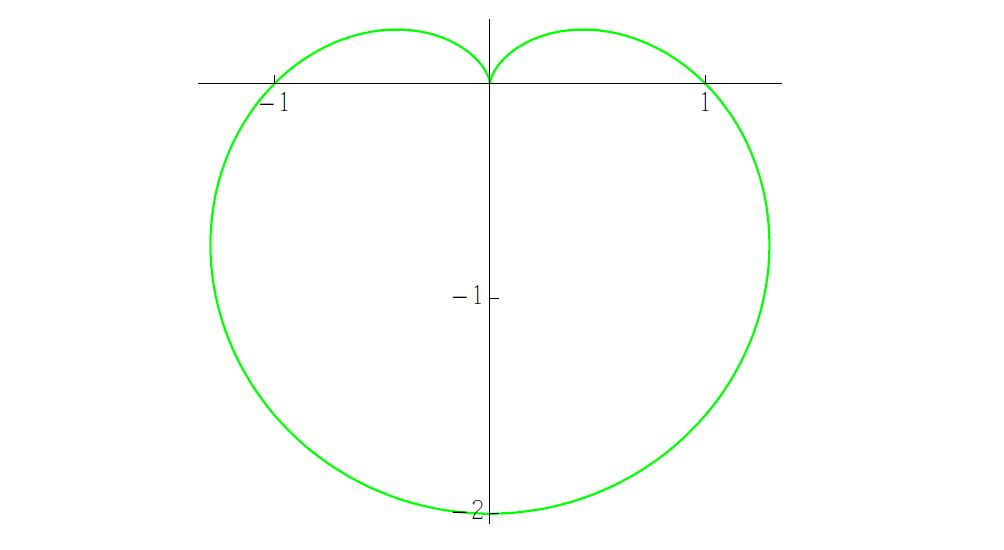
\includegraphics[width=0.8\textwidth]{cardioid.jpg}

\end{figure}
\end{spacing}
\end{frame}
\begin{frame}[c]{Smooth Curves}
\alert{2.3.16. Definition.} A curve $\mathcal{C}\subset V$ is said to be \emph{smooth} if there exists a parametrization $\gamma:I\to\mathcal{C}$ such that
\begin{enumerate}[(i)]
  \item $\gamma$ is continuously dif{}ferentiable on $\text{int}\,I$ and
  \item $D\gamma|_t\neq0$ for all $t\in\text{int}\,I$.
\end{enumerate}
A \emph{smooth reparametrization} is a reparametrization that is continuously
dif{}ferentiable with non-vanishing derivative in the interior of its domain.\\[6pt]
If $V=\R^n$, the Jacobian $D\gamma=\gamma'$ of a smooth curve $\gamma:I\to\R^n$ is given by
\[\gamma'(t)=\begin{pmatrix}
               \gamma_1'(t) \\
               \vdots \\
               \gamma_n'(t)
             \end{pmatrix},\qquad\qquad\qquad
             t\in\text{int}\,I.\]
\end{frame}
\begin{frame}[t]{Graphs of Functions as Curves}
\begin{spacing}{1.1}
Let us consider the case of the graph $\Gamma$ of a function $f:I\to\R,I\subset\R$ an interval: it is defined as the set
\[\Gamma=\{(x,y)\in\R^2:x\in I,y=f(x)\}.\]
This set can be regarded as a curve with parametrization
\[\gamma:I\to\R^2,\qquad\qquad\qquad t\mapsto\binom{t}{f(t)}.\]
\alert{2.3.17. Example.} Consider the function $f:\R\to\R,f(x)=x^2$. Its graph is just the curve parametrized by
\[\gamma(t)=\binom{\gamma_1(t)}{\gamma_2(t)}=\binom{t}{t^2}.\]
\end{spacing}
\end{frame}
\begin{frame}[t,allowdisplaybreaks,allowframebreaks]{Curves and Graphs of Functions}
\begin{spacing}{1}
\begin{figure}
  \centering
  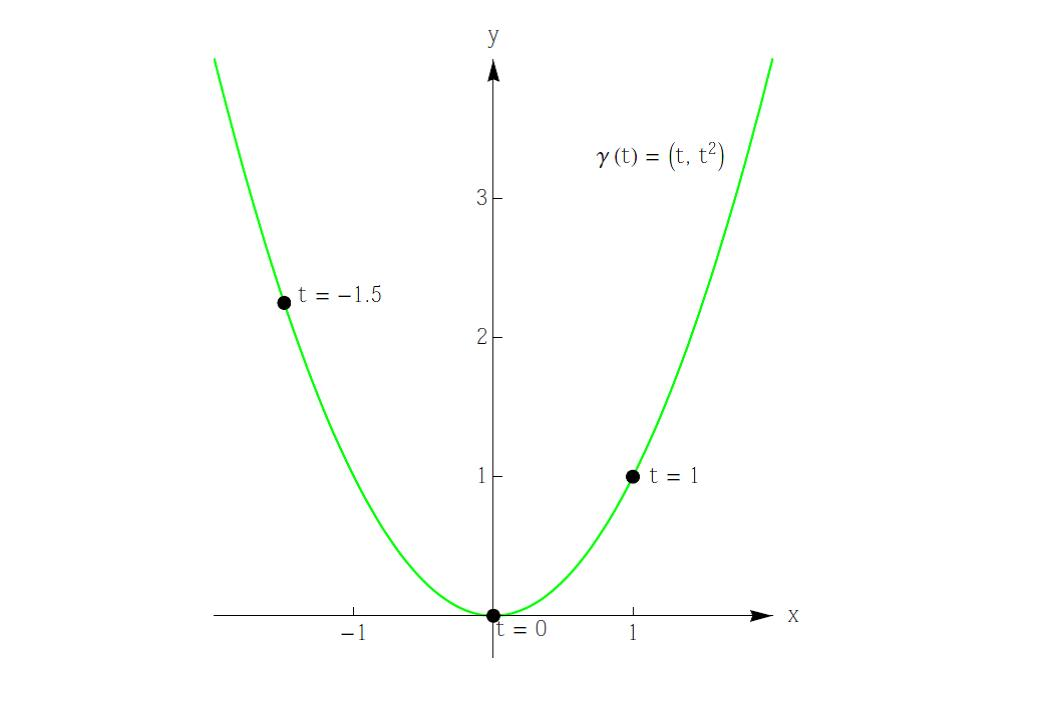
\includegraphics[width=0.8\textwidth]{45.jpg}

\end{figure}
\newpage
\begin{columns}[c,onlytextwidth]
\begin{column}{0.35\textwidth}
\includegraphics[width=\columnwidth,height=190pt]{46.jpg}
\end{column}
\begin{column}{0.65\textwidth}
By our previous considerations, $\gamma$ is dif{}ferentiable and
\[\gamma'(t)=\binom{\gamma_1'(t)}{\gamma_2'(t)}=\binom{1}{2t}.\]
The graph of $\gamma'$ is quite unspectacular.
\end{column}
\end{columns}
\end{spacing}
\end{frame}
\begin{frame}[t,allowdisplaybreaks,allowframebreaks]{Tangent Lines of Curves}
\begin{spacing}{1}
So what is the interpretation of $\gamma'$? If $\gamma=(t,f(t))$ parametrizes the graph function of some function $f$, then $\gamma'(t)=(1,f'(t))$. Recall that the derivative satisfies
\[\gamma(t_0+t)=\gamma(t_0)+\gamma'(t_0)t+o(t),\]
so $\gamma(t_0)+\gamma'(t_0)t$ is a linear approximation to the parametrization $\gamma$ at a point $t_0$.\\[5pt]
In fact, if $\mathcal{C}\subset\R^n$ is a curve and $p=\gamma(t_0)\in\mathcal{C}$, then
\[T_p\mathcal{C}=\{x\in\R^n:x=\gamma(t_0)
+\gamma'(t_0)t:t\in\R\}\]
gives the \emph{tangent line} to $\Gamma$ at $p$.
\newpage
Continuing from Example 2.3.17, we have the following tangent line $T_p\Gamma$ for $p=(1,1)$:
\begin{figure}
  \centering
  \includegraphics[width=0.9\textwidth,height=160pt]{47.jpg}
\end{figure}
\newpage
\begin{columns}[c,onlytextwidth]
\begin{column}{0.5\textwidth}
\alert{2.3.18. Example.} Consider the curve given by
\[\gamma\!:\,[0,8\pi]\to\R^3,~~\gamma(t)=\begin{pmatrix}
                                           t \\
                                           \cos t \\
                                           \sin t
                                         \end{pmatrix}\]
This curve is called a \emph{helix}.
\end{column}
\begin{column}{0.5\textwidth}
\includegraphics[width=\columnwidth]{85.jpg}
\end{column}
\end{columns}
\newpage
\begin{columns}[onlytextwidth]
\begin{column}{0.4\textwidth}
This is the graph of
\[\gamma'(t)=\begin{pmatrix}
               1 \\
               -\sin t \\
               \cos t
             \end{pmatrix}\]
\end{column}
\begin{column}{0.6\textwidth}
\includegraphics[width=\columnwidth]{86.jpg}
\end{column}
\end{columns}
\newpage
The tangent line makes sense as a linear approximation
\[\gamma(t_0+t)=\begin{pmatrix}
                  t_0 \\
                  \cos t_0 \\
                  \sin t_0
                \end{pmatrix}+\begin{pmatrix}
                                1 \\
                                -\sin t_0 \\
                                \cos t_0
                              \end{pmatrix}t+o(t)\]
\vspace*{-13pt}
\begin{figure}
  \centering
  \includegraphics[width=\textwidth,height=130pt]{50.jpg}

\end{figure}
\end{spacing}
\end{frame}
\begin{frame}[t,allowdisplaybreaks,allowframebreaks]{The Tangent Vector to a Curve}
\begin{spacing}{1.05}
\alert{2.3.19. Definition.} Let $\mathcal{C}^*\subset\R^n$ be an oriented smooth curve and $p\in\mathcal{C}^*$. Let $\gamma:I\to\R^n$ be a parametrization of $\mathcal{C}^*$. Then we define the \emph{unit tangent vector} to $\mathcal{C}^*$ at $p=\gamma(t)$ by
\begin{equation}\label{2.3.4}
  T\circ\gamma(t):=\frac{\gamma'(t)}{\|\gamma'(t)\|},
  \qquad\qquad\quad t\in\text{int}\,I.
\end{equation}
This defines the \emph{tangent vector field} $T:\mathcal{C}^*\to\R^n$ on $\mathcal{C}$.\\[5pt]
Note that \eqref{2.3.4} does not depend on the parametrization $\gamma$, as long as $\gamma$ corresponds to the orientation of $\mathcal{C}^*$.\\[5pt]
In fact, suppose $\gamma:I\to\mathcal{C},\widetilde{\gamma}:J\to
\mathcal{C}$ are two smooth parametrizations connected by a reparametrization $r:J\to I$ so that $\widetilde{\gamma}=\gamma\circ r$. Let $p\in\mathcal{C}$ satisfy $p=\gamma(t)=\widetilde{\gamma}(\tau),t=r(\tau)$.\\
Then
\[\widetilde{\gamma}'(\tau)=\frac{d}{d\tau}\gamma(r(\tau))=\gamma'(r(\tau))r'(\tau)=\gamma'(t)r'(\tau).\]
\newpage
Hence,
\begin{equation}\label{2.3.5}
T\circ\widetilde{\gamma}(\tau)=\frac{\widetilde{\gamma}(\tau)}{\|\widetilde{\gamma}'(\tau)\|}=\frac{r'(\tau)}{|r'(\tau)|}
\frac{\gamma'(t)}{\|\gamma'(t)\|}=\frac{r'(\tau)}{|r'(\tau)|}T\circ\gamma(t).
\end{equation}
We see that if $r$ is orientation-preserving, then $r'(t)>0$ and the tangent vector
is the same when calculated using $\gamma$ as when using $\widetilde{\gamma}$. If $r$ is
orientation-reversing, the tangent vector reverses direction. This proves that \eqref{2.3.4} defines a unique tangent vector for an oriented curve.
\end{spacing}
\newpage
\begin{spacing}{0.6}
\alert{2.3.20. Example.} Consider the circle of radius $R$ in $\R^2$,
\[\mathcal{C}:=\{x\in\R^2:x_1^2+x_2^2=R^2\}.\]
By choosing the parametrization
\[\gamma:[0,2\pi)\to\mathcal{C},\qquad\qquad\quad
\gamma(t)=\binom{R\cos t}{R\sin t}\]
we endow $\mathcal{C}$ with a positive (counter-clockwise) orientation. The unit
tangent vector at $\gamma(t)$ is then given by
\[T\circ\gamma(t)=\frac{\gamma'(t)}{\|\gamma'(t)\|}=\frac{1}{R}
\binom{-R\sin t}{R\cos t}=\binom{-\sin t}{\cos t}.\]
Thus, if $p=(p_1,p_2)\in\mathcal{C}$, then
\[T(p)=\frac{1}{R}\binom{-p_2}{p_1}.\]
Hence $T(p)\perp p$.
\end{spacing}
\end{frame}
\begin{frame}[t]{Rate of Change of the Tangent Vector}
\begin{spacing}{1.2}
In order to gain more insight into the geometric properties of a curve, we
will study the rate of change of the tangent vector as it "travels" along a
curve. We assume from now on that
\begin{itemize}
  \item $V$ is a real inner product space and
  \item $\mathcal{C}\subset V$ has a parametrization $\gamma$ such that $\gamma''$ exists and $\gamma''\neq0$.
\end{itemize}
We call such a $\mathcal{C}$ a \emph{smooth $C^2$-curve} and $\gamma$ a $C^2$-parametrization.\\[5pt]
We are interested in
\begin{equation}\label{2.3.6}
  \frac{d}{dt}\left(T\circ\gamma(t)\right).
\end{equation}
Now $T\circ\gamma$ itself parametrizes a curve $\mathcal{T}$, so \eqref{2.3.6} gives the tangent vector of $\mathcal{T}$ at $T\circ\gamma(t)$. Moreover, since $\|T\|=1$ we see that
\[\mathcal{T}\subset S=\{x\in V:\|x\|=1\}.\]
\end{spacing}
\end{frame}
\begin{frame}[t,allowdisplaybreaks,allowframebreaks]{The Normal Vector of a Curve}
\begin{spacing}{1.05}
Just as in Example 2.3.20, this implies that \eqref{2.3.6} is perpendicular to $T\circ\gamma(t)$:
\begin{equation}\label{2.3.7}
  \begin{split}
       &1=\|T\circ\gamma(t)\|^2=\scp{T\circ\gamma(t)}{T\circ\gamma(t)}  \\
     \Rightarrow~~~ &0=\frac{d}{dt}\scp{T\circ\gamma(t)}{T\circ\gamma(t)}
     =2\scp{(T\circ\gamma)'(t)}{T\circ\gamma}
  \end{split}
\end{equation}
 \\[18pt]
\alert{2.3.21. Definition.} Let $\mathcal{C}\subset V$ be a smooth $C^2$-curve. Let $\gamma:I\to V$ be a smooth $C^2$-parametrization of $\mathcal{C}$. Then the unit normal vector $N:\mathcal{C}\to\R$ is defined by
\begin{equation}\label{2.3.8}
  N\circ\gamma(t):=\frac{(T\circ\gamma)'(t)}{\|(T\circ\gamma)'(t)\|},
  \qquad\qquad\quad t\in\text{int}\,I.
\end{equation}
\newpage
The unit normal vector does not depend on $\gamma$, not even up to orientation: suppose $\gamma:I\to\mathcal{C},\widetilde{\gamma}:J\to\mathcal{C}$ are two $C^2$-parametrizations connected by a $C^2$-reparametrization $r:J\to I$ so that $\widetilde{\gamma}=\gamma\circ r$. Let $p\in\mathcal{C}$ satisfy $p=\gamma(t)=\widetilde{\gamma}(\tau),\,
t=r(\tau)$.\\
By \eqref{2.3.5},
\[T\circ\widetilde{\gamma}(\tau)=\frac{r'(\tau)}{|r'(\tau)|}
T\circ\gamma(t).\]
Suppose that $r$ is orientation-reversing. Then
\[\frac{d}{d\tau}T\circ\widetilde{\gamma}(\tau)=-\frac{d}{d\tau}
T\circ\gamma(r(\tau))=-(T\circ\gamma)'(r(\tau))r'(\tau)\]
and
\[N\circ\widetilde{\gamma}(\tau)=-\frac{r'(\tau)}{|r'(\tau)|}
\frac{(T\circ\gamma)'(t)}{\|(T\circ\gamma)'(t)\|}=
\frac{(T\circ\gamma)'(t)}{\|(T\circ\gamma)'(t)\|}.\]
Of course, if $r$ is orientation-preserving, the proof is similar.
\end{spacing}
\newpage
\begin{spacing}{0.4}
\alert{2.3.22. Example.} We return to Example 2.3.20 and study the circle of radius $R$ in $\R^2$ with parametrization
\[\gamma:[0,2\pi)\to\mathcal{C},\qquad\qquad\quad
\gamma(t)=\binom{R\cos t}{R\sin t}.\]
The unit tangent vector at $\gamma(t)$ is given by
\[T\circ\gamma(t)=\binom{-\sin t}{\cos t}\qquad\Rightarrow\qquad(T\circ\gamma)'(t)
=\binom{-\cos t}{-\sin t}\]
and $\|(T\circ\gamma)'(t)\|=1$. Then
\[N\circ\gamma(t)=\frac{(T\circ\gamma)'(t)}{\|(T\circ\gamma)'(t)\|}=\binom{-\cos t}{-\sin t}\]
Thus, if $p=(p_1,p_2)\in\mathcal{C}$, then
\[N(p)=-\frac{1}{R}p\]
and we see $N(p)\perp T(p)$.
\end{spacing}
\end{frame}
\begin{frame}[t,allowdisplaybreaks,allowframebreaks]{Physical interpretation of Tangent and Normal Vectors}
\begin{spacing}{1}
If the parametrization $\gamma(t)$ describes the trajectory of a particle (point
mass) and the curve $\mathcal{C}\subset\R^3$ the travelled path in space, then $\gamma'(t)$ gives
the velocity of the particle.\\[10pt]
Hence, the unit tangent vector $T$ gives the direction of the velocity and
the unit normal vector $N$ gives the direction of the change in $T$. By
Newton's laws, a force $F$ acting on a particle causes an acceleration, i.e., a
change in $\gamma'(t)$. The acceleration will have a component parallel to $T$ and
a component orthogonal to $T$, given by $N$. Then $F$, proportional to the
acceleration, can be decomposed as
\[F=F_T+F_N\qquad\text{where}\qquad
F_T=\scp{F}{T}T,\qquad F_N=\scp{F}{N}N.\]
The plane spanned by $N$ and $T$ is called the osculating plane (the latin
word \emph{osculum} means "to kiss"). It lies geometrically closest to the curve
at the point where $T$ and $N$ are calculated.
\newpage
\alert{2.3.23. Example.} Consider a mathematical pendulum, where a mass point swings at the length of a string under the influence of gravity $F_g=mg$.\\[9pt]
\begin{columns}[onlytextwidth]
\begin{column}{0.4\textwidth}
\includegraphics[width=\columnwidth,height=170pt]{87.jpg}
\end{column}
\begin{column}{0.6\textwidth}
The trajectory is a circle (segment) centered
at the fulcrum of the pendulum. If we place
the origin of our coordinate system at this
fulcrum, the tangent vector will be orthogonal
to the position of the mass point, pointing in
the direction of movement. We obtain
\[F_T:=\langle F,T\rangle T=m\langle g,T\rangle T=mg\sin\theta T,\]
\[F_N:=\langle F,N\rangle N=m\langle g,N\rangle N=mg\cos\theta N,\]
where $\theta$ is shown in the image. The normal component $F_N$ induces tension in the string, while $F_T$ causes acceleration of the mass point along its trajectory.
\end{column}
\end{columns}
\end{spacing}
\end{frame}
\begin{frame}[t,allowdisplaybreaks,allowframebreaks]{Curve Length}
\begin{spacing}{1.1}
Consider a simple curve $\mathcal{C}\subset V$ parametrized by $\gamma:[a,b]\to V$, where $(V,\|\cdot\|)$ is a normed vector space. Then a natural approximation to the length of $\gamma$, which \emph{will} depend on the norm used, is found by taking a partition $\mathcal{P}=(a_0,\ldots,a_n)$ of $[a,b]$ and considering the lengths of the straight line segments joining $(a_{i-1},\gamma(a_{i-1})$ to $(a_i,\gamma(a_i)),i=1,\ldots,n$.\\[4pt]
The sum of the lengths of these line segments is given by
\[\ell_\mathcal{P}(\mathcal{C})=\sum_{i=1}^{n}
\|\gamma(a_i)-\gamma(a_{i-1})\|.\]
We will say that a curve has a length if there exists an upper bound to
these lengths. Note that $\ell_\mathcal{P}(\mathcal{C})$ is of course independent of the parametrization $\gamma$, since only the actual points $\gamma(a_i)\in\mathcal{C}$ are used in this definition.
\end{spacing}
\newpage
\begin{spacing}{0.85}
\alert{2.3.24. Definition.} Let $(V,\|\cdot\|)$ be a normed vector space and $\mathcal{C}\subset V$ an open curve. Then we say that $\mathcal{C}$ is \emph{rectifiable} if
\[\ell(\mathcal{C}):=\sup\limits_{\text{partitions}\,\mathcal{P}}\ell_\mathcal{P}(\mathcal{C})\]
exists. We then call $\ell(f)$ the \emph{curve length} or \emph{arc length} of $\mathcal{C}$.\\[4pt]
\alert{2.3.25. Theorem.} Let $\mathcal{C}\subset V$ be a smooth and open curve with parametrization $\gamma:[a,b]\to\mathcal{C}$. Then $\mathcal{C}$ is rectifiable if and only if
\[\int_{a}^{b}\|\gamma'(t)\|dt<\infty.\]
Furthermore, if $\mathcal{C}$ is rectifiable,
\[\ell(\mathcal{C})=\int_{a}^{b}\|\gamma'(t)\|dt,\]
where the right-hand side is independent of $\gamma$.
\end{spacing}
\newpage
\begin{spacing}{1.05}
\alert{2.3.26. Example.} Consider the helix segment $\mathcal{C}$ given by the graph of
\[\gamma:[0,2\pi]\to\R^3,\qquad\qquad
\gamma(t)=\begin{pmatrix}
            \alpha t \\
            R\cos t \\
            R\sin t
          \end{pmatrix},\qquad\alpha,R>0.\]
The length of $\mathcal{C}=\gamma([0,2\pi])$ is given by
\begin{equation*}
  \begin{split}
     \ell(\mathcal{C}) &=\int_{0}^{2\pi}\|\gamma'(t)\|dt
     =\int_{0}^{2\pi}\sqrt{\alpha^2+(-R\sin t)^2+R^2\cos^2t}dt \\
       &=2\pi\sqrt{\alpha^2+R^2}.
  \end{split}
\end{equation*}
\alert{2.3.27. Remark.} Definition 2.3.24 and Theorem 2.3.25 refer to open
curves. To find the length of a closed curve, we express it as the disjoint
union of two simple curves and find their lengths separately.
\newpage
\alert{Proof of Theorem 2.3.25.}\\
We first show that the value of the integral
\[\int_{a}^{b}\|\gamma'(t)\|dt\]
does not depend on the parametrization $\gamma$. Let $\mathcal{C}\subset V$ be a smooth curve and $\gamma:[a,b]\to\mathcal{C}$ a parametrization of $\mathcal{C}$. Let $\widetilde{\gamma}:[\alpha,\beta]\to\mathcal{C}$ be some other parametrization and let $r:[\alpha,\beta]\to[a,b]$ be a smooth reparametrization, so that
\[\widetilde{\gamma}(\tau)=\gamma(r(\tau))\]
Suppose that $r$ is orientation-preserving. Then $r(\alpha)=a$ and $r(\beta)=b$.
\newpage
\alert{Proof (continued).}\\
Let $t=r(\tau)$ so $dt=r'(\tau)d\tau$. Furthermore,
\[\widetilde{\gamma}'(\tau)=\left(\gamma\circ
r(\tau)\right)'=\gamma'(r(\tau))r'(\tau)
\qquad\Leftrightarrow\qquad\gamma'(r(\tau))=
\frac{\widetilde{\gamma}'(\tau)}{r'(\tau)}\]
Thus, substituting $t=r(\tau)$,
\begin{equation*}
  \begin{split}
     \int_{a}^{b}\|\gamma'(t)\|dt &=\int_{\alpha}^{\beta}\|\gamma'(r(\tau))\|r'(\tau)d\tau
     =\int_{\alpha}^{\beta}\left\|\frac{\widetilde{\gamma}(\tau)}{r'(\tau)}
     \right\|r'(\tau)d\tau \\
       &=\int_{\alpha}^{\beta}\frac{\|\widetilde{\gamma}(\tau)\|}{|r'(\tau)|}r'(\tau)d\tau
       =\int_{\alpha}^{\beta}\|\widetilde{\gamma}'(\tau)\|d\tau,
  \end{split}
\end{equation*}
where we have used that $r$ is increasing, i.e., $r'(\tau)>0$. This proves that $\int_{a}^{b}\|\gamma'(t)\|dt$ is independent of the parametrization $\gamma$.
\newpage
\alert{Proof (continued).}\\
Now, for any partition $\mathcal{P}$ of $[a,b]$ and any parametrization $\gamma$ we have
\begin{equation*}
  \begin{split}
     \ell_\mathcal{P}(\mathcal{C}) &=\sum_{i=1}^{n}\|\gamma(a_i)-\gamma
     (a_{i-1})\|\\
       &=\sum_{i=1}^{n}\Big\|\int_{a_{i-1}}^{a_i}
       \gamma'(t)dt\Big\|  \\
       &\leq\sum_{i=1}^{n}\int_{a_{i-1}}^{a_i}\|\gamma'(t)
       \|dt  \\
       &=\int_{a}^{b}\|\gamma'(t)\|dt.
  \end{split}
\end{equation*}
Hence, $\ell(\mathcal{C})\leq\int_{a}^{b}\|\gamma'(t)\|dt$.
\newpage
\alert{Proof (continued).}\\
Proving the converse inequality is slightly more dif{}ficult. We first establish
three preliminary estimates. We will use the fact that since $\mathcal{C}$ is smooth, $\gamma':[a,b]\to V$ is continuous and hence uniformly continuous on $[a,b]$ (see Theorem 2.1.38). Fix $\varepsilon>0$.
\begin{enumerate}[(i)]
  \item Choose a $\delta>0$ such that
      \[|t-\tau|<\delta\qquad\Rightarrow\qquad
      \|\gamma'(t)-\gamma'(\tau)\|<\frac{\varepsilon}{2(b-a)}\]
      for all $t,\tau\in[a,b]$.
\end{enumerate}
\newpage
\alert{Proof (continued).}
\begin{itemize}
  \item[(ii)] Consider the function $f:[a,b]\to\R,f(t)=\|\gamma'(t)\|$. Since $\gamma$ is smooth, $f$ is continuous and we can find a step function that uniformly approximates $f$. In fact, there is a $0<\delta_1<\delta$ and a partition $\mathcal{P}=(a_0,\ldots,a_n)$ with $a_i-a_{i-1}<\delta_1,i=1,\ldots,n$, of $[a,b]$ such that
      \[\left|\int_{a}^{b}\|\gamma'(t)\|dt-\sum_{i=1}^{n}
      (a_i-a_{i-1})\|\gamma'(a_{i-1})\|\right|<\varepsilon/2\]
\end{itemize}
\newpage
\alert{Proof (continued).}\\
\begin{itemize}
  \item[(iii)] For any $t\in(a,b)$ and $h<\delta$ with $t+h\in[a,b]$,
  \begin{equation*}
    \begin{split}
       \Big\|\frac{\gamma(t+h)-\gamma(t)}{h}-\gamma'(t)\Big\| &=\Big\|\frac{1}{h}\int_{t}^{t+h}\gamma'(\tau)d\tau-\gamma'(t)\Big\| \\
         &=\Big\|\frac{1}{h}\int_{t}^{t+h}\left(\gamma'(\tau)-\gamma'(t)\right)d\tau\Big\|  \\
         &\leq\frac{1}{h}\int_{t}^{t+h}\|\gamma'(\tau)-\gamma'(t)\|d\tau  \\
         &\leq\frac{h}{h}\sup\limits_{\tau\in[t,t+h]}\|\gamma'(\tau)-\gamma'(t)\|<\frac{\varepsilon}{2(b-a)}.
    \end{split}
  \end{equation*}
This implies $\displaystyle \|\gamma'(t)\|\leq\left\|\frac{\gamma(t+h)-\gamma(t)}{h}\right\|+\frac{\varepsilon}{2(b-a)}.$
\end{itemize}
\newpage
\alert{Proof (continued).}\\
We then have
\begin{equation*}
  \begin{split}
     \int_{a}^{b}\|\gamma'(t)\|dt &\leq\sum_{i=1}^{n}(a_i-a_{i-1})\|\gamma'(a_{i-1})\|
     +\frac{\varepsilon}{2} \\
       &\leq\sum_{i=1}^{n}(a_i-a_{i-1})\Big\|\frac{\gamma(a_i)-\gamma(a_{i-1})}{a_i-a_{i-1}}\Big\|
       +\frac{\varepsilon}{2(b-a)}(b-a)+\frac{\varepsilon}{2}  \\
       &\leq\sum_{i=1}^{n}(a_i-a_{i-1})\frac{\|\gamma(a_i)-\gamma(a_{i-1})\|}{|a_i-a_{i-1}|}+\varepsilon  \\
       &=\sum_{i=1}^{n}\|\gamma(a_i)-\gamma(a_{i-1})\|+\varepsilon
       =\ell_\mathcal{P}(\mathcal{C})+\varepsilon  \\
       &\leq\ell(\mathcal{C})+\varepsilon
  \end{split}
\end{equation*}
\vspace*{-5pt}
Letting $\varepsilon\to0$, we obtain the desired inequality.\multido{}{6}{\qquad}\quad{$\square$}
\newpage
We can now express the total curve length by
\[\ell(\mathcal{C})=\int_{a}^{b}\|\gamma'(t)\|dt.\]
More generally, we can define a \emph{length function}
\begin{equation}\label{2.3.9}
  (\ell\circ\gamma)(s)=\int_{a}^{s}\|\gamma'(t)\|dt
\end{equation}
so that $\ell\circ\gamma(b)=\ell(\mathcal{C})$.\\[6pt]
The function
\[\ell\circ\gamma:[a,b]\to[0,\infty)\]
associates to each value of $t$ the length of the curve at $\gamma(t)$. Since the integral \eqref{2.3.9} is strictly monotonic, $\ell\circ\gamma$ is strictly increasing and hence bijective.
\end{spacing}
\newpage
\begin{spacing}{0.95}
\alert{2.3.28. Example.} We return to Example 2.3.20 and study the circle of radius $R$ in $\R^2$ with parametrization
\[\gamma:[0,2\pi)\to\mathcal{C},\qquad\qquad
\gamma(t)=\binom{R\cos t}{R\sin t}.\]
The curve length is given by
\[(\ell\circ\gamma)(s)=\int_{0}^{s}\|\gamma'(t)\|dt
=\int_{0}^{s}R\,dt=Rs.\]
Thus, for $p=(p_1,p_2)\in\mathcal{C}$, we can read of{}f
\[\ell(p)=R\cdot\arctan\frac{p_2}{p_1}.\]
where the arctangent is understood in the sense of \eqref{2.3.1}; i.e., the
appropriate branch is chosen depending on the signs of $p_1$ and $p_2$.
\end{spacing}
\end{frame}
\begin{frame}[t]{Parametrization Through Curve Length}
\begin{spacing}{1}
The map $\ell:\mathcal{C}^*\to[0,\infty)$ is bijective, since its inverse is given by
\[\ell^{-1}=\gamma\circ(\ell\circ\gamma)^{-1}.\]
If $s=\ell(p)$ is the curve length at $p\in\mathcal{C}^*$, then $p=\ell^{-1}(s)$ is the unique point in $\mathcal{C}$ associated to this curve length.\\[5pt]
In other words, once we fix an orientation of a simple curve $\mathcal{C}$, the curve
length determines all other points of $\mathcal{C}^*$ uniquely. This means that we can
use the curve length as a \emph{natural parametrization} of $\mathcal{C}$, i.e., we can
parametrize $\mathcal{C}$ using
\[\gamma=\ell^{-1}:I\to\mathcal{C},\qquad
\qquad\quad\text{int}\,I=(0,\ell(\mathcal{C})).\]
If we want to parametrize closed curves through curve length, we must fix
an "initial point" in some fashion.
\end{spacing}
\end{frame}
\begin{frame}[t,allowdisplaybreaks,allowframebreaks]{Curvature}
\begin{spacing}{1}
We are interested in the rate of change of the direction of the tangent
vector to a curve. However, while $T$ does not depend on $\gamma$, if we simply dif{}ferentiate $T\circ\gamma(t)$, the derivative \emph{will} depend on $\gamma$. In order to obtain a purely geometric measure for the rate of change of $T$, we need to settle on a "canonical" parametrization. Luckily, we have just developed one:
parametrization using curve length. This parametrization takes into
account only the specific geometric properties of the curve.\\[5pt]
\alert{2.3.29. Definition.} The \emph{curvature} of a smooth $C^2$-curve $\mathcal{C}\subset V$ is
\[\kappa:\mathcal{C}\to\R,\qquad\quad
\kappa\circ\ell^{-1}(s):=\left\|\frac{d}{ds}
\left(T\circ\ell^{-1}(s)\right)\right\|\]
where $T$ is the unit tangent vector and $\ell^{-1}:I\to\mathcal{C}$ is the curve length parametrization of $\mathcal{C}$.\\[5pt]
Note that, like the unit normal vector $N$, $\kappa$ also does not depend on the orientation of $\mathcal{C}$.
\newpage
If we have a parametrization $\gamma:I\to\mathcal{C}$ of $\mathcal{C}$ (which is not the curve length), then by the chain rule
\[\left.\frac{d(T\circ\gamma)}{dt}\right|_t=
\left.\frac{d(T\circ\ell^{-1})}{ds}\right|_{s=\ell\circ\gamma(t)}
\left.\frac{d(\ell\circ\gamma)}{dt}\right|_t\]
and so we obtain for the curvature on $I$
\begin{equation}\label{2.3.10}
  \kappa\circ\gamma(t)=\left\|\frac{d(T\circ\gamma)}{dt}\Big|_t\left(
  \frac{d(\ell\circ\gamma)}{dt}\Big|_t\right)^{-1}\right\|
  =\frac{\|(T\circ\gamma)'(t)\|}{\|\gamma'(t)\|},
\end{equation}
where we have used \eqref{2.3.9}.\\[5pt]
\alert{2.3.30. Remark.} For technical reasons we have defined curvature only for
simple open curves. Of course, the curvature is a local property, and if we
are interested in the curvature at point, we may simply look at a simple
and open subsection of the curve that includes this point.
\newpage
\alert{2.3.31. Example.} We returnto Example 2.3.20 and study the circle of radius $R$ in $\R^2$ with parametrization
\[\gamma:[0,2\pi)\to\mathcal{C},\qquad\qquad
\gamma(t)=\binom{R\cos t}{R\sin t}.\]
We have
\[T\circ\gamma(t)=\binom{-\sin t}{\cos t},\qquad\qquad\quad
\ell\circ\gamma(t)=Rt.\]
Then by \eqref{2.3.10} we have
\[\kappa\circ\ell^{-1}(t)=\left\|\frac{d(T\circ\gamma)}{dt}\Big|_t
\left(\frac{d(\ell\circ\gamma)}{dt}\Big|_t\right)^{-1}\right\|=
\left\|\binom{-\cos t}{-\sin t}R^{-1}\right\|=\frac{1}{R}.\]
Thus, the curvature of circle is constant and equal to the inverse of its
radius.
\end{spacing}
\end{frame}
\begin{frame}[t,allowdisplaybreaks,allowframebreaks]{Curvature in $\R^3$}
\begin{spacing}{1}
For curves $\gamma:I\to\R^3$ there is a useful geometric formula for the curvature.\\[5pt]
\alert{2.3.32. Lemma.} Let $\mathcal{C}\subset\R^3$ be a smooth $C^2$-curve with parametrization $\gamma:I\to\mathcal{C}$. Then
\begin{equation}\label{2.3.11}
  \kappa\circ\gamma(t)=\frac{\|\gamma'(t)\times\gamma''(t)\|}{\|\gamma'(t)\|^3}
\end{equation}
\alert{Proof.}\\
From \eqref{2.3.4} we have $\gamma'(t)=\|\gamma'(t)\|(T\circ\gamma)(t)$. The product rule yields
\[\gamma''(t)=\frac{d\|\gamma'(t)\|}{dt}(T\circ\gamma)(t)
+\|\gamma'(t)\|(T\circ\gamma)'(t).\]
Now, since $T\times T=0$ and $T\perp T'$ we have
\begin{equation}\label{2.3.12}
  \begin{split}
     \|\gamma'(t)\times\gamma''(t)\| &=\|\gamma'(t)\|^2\cdot\left\|(T\circ\gamma)(t)\times
     (T\circ\gamma)'(t)\right\| \\
       &=\|\gamma'(t)\|^2\cdot\|(T\circ\gamma)'(t)\|
  \end{split}
\end{equation}
\end{spacing}
\newpage
\begin{spacing}{1.2}
\alert{Proof (continued).}\\
From
\[\|\gamma'(t)\times\gamma''(t)\|=\|\gamma'(t)\|^2\cdot
\|(T\circ\gamma)'(t)\|\]
we obtain
\[\kappa\circ\gamma(t)=\frac{\|(T\circ\gamma)'(t)\|}{\|\gamma'(t)\|}
=\frac{\|\gamma'(t)\times\gamma''(t)\|}{\|\gamma'(t)\|^3}\]
\begin{flushright}
  $\square$
\end{flushright}
\end{spacing}
\end{frame}
\subsection{Potential Functions}
\begin{frame}[c]
\begin{spacing}{2.5}
\tableofcontents[sectionstyle=hide,subsectionstyle=show/shaded/hide]
\end{spacing}
\end{frame}
\begin{frame}[t]{Potentials}
\begin{spacing}{1.05}
A map $f:\Omega\to\R$ where $\Omega\subset\R^n$ is called a scalar function or a \emph{potential}. Physically, if $n=3$, a potential assigns to each point in space a scalar value. Examples include temperature, pressure or height.\\[5pt]
The Jacobian of a dif{}ferentiable potential is given by
\[Df|_x=\begin{pmatrix}
          \frac{\partial f}{\partial x_1}\big|_x & \cdots & \frac{\partial f}{\partial x_n}\big|_x
        \end{pmatrix}.\]
The row vector $Df|_x$ may be regarded as a linear map $Df|_x:\R^n\to\R$,
\[Df|_xy=\begin{pmatrix}
          \frac{\partial f}{\partial x_1}\big|_x & \cdots & \frac{\partial f}{\partial x_n}\big|_x
        \end{pmatrix}\begin{pmatrix}
                       y_1 \\
                       \vdots \\
                       y_n
                     \end{pmatrix}=\left.\sum_{i=1}^{n}y_i\frac{\partial f}{\partial x_i}\right|_x\]
Thus $Df|_x\in(\R^n)^*$, the dual space of $\R^n$ (see Examples 1.4.6 ii)).
\end{spacing}
\end{frame}
\begin{frame}[t]{Coordinate Maps}
\begin{spacing}{1.05}
Classically, we considered $x_j(1\leq j\leq n)$ as a coordinate of the vector $x=(x_1,\ldots,x_n)\in\R^n$. We now introduce a dif{}ferent interpretation. Define the map
\[\R^n\to\R,\qquad\qquad\quad
x=\begin{pmatrix}
    x_1 \\
    \vdots \\
    x_n
  \end{pmatrix}\mapsto x_j.\]
This map is clearly linear; it is the \emph{coordinate map} that assigns to $x\in\R^n$ its coordinate $x_j$. We denote this map by $x_j$ also; hence $x_j:x\mapsto x_j$ or $x_j(x)=x_j$. The dual meaning of $x_j$ as a map and the value of this map is very convenient. In fact, the entire discipline of \emph{dif{}ferential geometry} hinges
on exploiting this ambiguity.\\[6pt]
The derivative of the map $x_j$ is given by
\setcounter{equation}{0}
\begin{equation}\label{2.4.1}
  dx_j=(0,\ldots,0,\mathop{1}_{\begin{subarray}
                                 ~\uparrow\\
                                 j
                               \end{subarray}},0,\ldots,0)
\end{equation}
\end{spacing}
\end{frame}
\begin{frame}[t]{The Dif{}ferential and the Gradient}
\begin{spacing}{1.05}
Note that we have written $dx_j$ instead of $Dx_j$; this is traditional. The derivative of a scalar map $f$ is also called a \emph{dif{}ferential} and written $df$ instead of $Df$. Note also that $dx_j|_x$ does not depend on $x$. Therefore, we have
\[df|_x=\begin{pmatrix}
          \frac{\partial f}{\partial x_1}\big|_x & \cdots & \frac{\partial f}{\partial x_n}\big|_x
        \end{pmatrix}=\left.\frac{\partial f}{\partial x_1}\right|_x dx_1+\cdots+\left.\frac{\partial f}{\partial x_n}\right|_x dx_n\]
Each dif{}ferential $dx_j=e_j^*$ is the dual basis vector to the standard basis vector $e_j$ with respect to the euclidian scalar product.\\[5pt]
The transpose of the Jacobian is the \emph{gradient},
\[\nabla f(x):=(J_f(x))^T=\begin{pmatrix}
                            \frac{\partial f}{\partial x_1}\big|_x \\
                            \vdots
                             \\
                            \frac{\partial f}{\partial x_n}\big|_x
                          \end{pmatrix}\]
The triangle is pronounced "nabla"; we will study the gradient more closely later.
\end{spacing}
\end{frame}
\begin{frame}[t,allowdisplaybreaks,allowframebreaks]{The Directional Derivative}
\begin{spacing}{1}
\alert{2.4.1. Definition.} Let $\Omega\subset\R^n$ be an open set, $f:\Omega\to\R$ continuous and $h\in\R^n,\,\|h\|=1$, be a unit vector. Then the \emph{directional derivative $D_hf$} in the direction $h$ is defined by
\begin{equation}\label{2.4.2}
D_hf|_x:=\frac{d}{dt}f(x+th)\Big|_{t=0}.
\end{equation}
The directional derivative has the following interpretation: if
$\gamma(t)=x+th,t\in[0,1]$, parametrizes the straight line segment joining $x$ and $x+h$, then $D_hf$ is simply the derivative of $f\circ\gamma$.\\
Hence,
\begin{quote}
  The directional derivative $D_hf|_x$ is the derivative of $f$ at $x$ along the line segment joining $x$ and $x+h$.
\end{quote}
\vspace*{-3pt}
Another way of stating this is
\begin{quote}
  The directional derivative $D_hf|_x$ gives the slope of the tangent line of $f$ at $x$ in the direction of $h$.
\end{quote}
\newpage
It is essential that $\|h\|=1$, otherwise the slope will not be scaled correctly!
\begin{figure}
  \centering
  \includegraphics[width=0.8\textwidth]{52.jpg}

\end{figure}
\newpage
We note that the tangent line of $f:\R^n\to\R$ at $x$ in the direction $h$ is given by
\begin{equation}\label{2.4.3}
  t_{f,x;h}(s)=\binom{x+sh}{f(x)+D_hf|_xs},\qquad\qquad
  s\in\R,
\end{equation}
where $h\in\R^n$ (so the above vector is a "block vector" with $n+1$ entries).\\[5pt]
For function $f:\R^2\to\R$ the directional derivative is sometimes specified through the angle $\theta$. This understood to mean that
\[h=\binom{\cos\theta}{\sin\theta}.\]
Note that the directional derivative is a \emph{number}, in contradistinction to
the derivative. Thus it should perhaps be more properly known as the
"directional slope."
\newpage
\alert{2.4.2. Example.} Let $f:\R^2\to\R,f(x_1,x_2)=x_1^2-4x_2$. Then the directional derivative of $f$ at $x$ in the direction is
\begin{equation*}
  \begin{split}
     D_hf|_x &=\left.\frac{d}{dt}f(x+th)\right|_{t=0}
     =\left.\frac{d}{dt}\left((x_1+th_1)^2-4(x_2+th_2)\right)\right|_{t=0} \\
       &=2h_1(x_1+th_1)-4h_2|_{t=0}  \\
       &=2h_1x_1-4h_2.
  \end{split}
\end{equation*}
For $h=(\nicefrac{1}{\sqrt{2}},\nicefrac{1}{\sqrt{2}})$ (or $\theta=\nicefrac{\pi}{4}$) we would have
\[D_hf|_x=\sqrt{2}x_1-2\sqrt{2}.\]
At $x=(0,0)$, the directional derivative in direction $h$ is
\[D_hf|_{x=0}=-2\sqrt{2}\]
\end{spacing}
\newpage
\begin{spacing}{1.2}
Suppose that $f$ is dif{}ferentiable. If $\gamma(t)=x+th,t\in[0,1]$, parametrizes the straight line segment joining $x$ and $x+h$, then by the chain rule
\[D_hf|_x=\left.\frac{d}{dt}f(x+th)\right|_{t=0}
=Df|_{x+th}h\Big|_{t=0}=Df|_xh\]
so
\begin{equation}\label{2.4.4}
  D_hf|_x=Df|_xh=\scp{\nabla f(x)}{h}.
\end{equation}
This is a useful expression for calculating the directional derivative, but it
supposes that $f$ is dif{}ferentiable. In practice, \eqref{2.4.4} will be valid if the
partial derivatives if $f$ exist and are continuous at $x$.
\newpage
\alert{2.4.3. Example.} Returning to Example 2.4.2, we have
\[\nabla f(x)=\binom{2x_1}{-4}\]
Since the partial derivatives are continuous,
\[D_hf|_x=\scp{\nabla f(x)}{h}=\scp{\binom{2x_1}{-4}}{\binom{h_1}{h_2}}
=2x_1h_1-4h_2.\]
This coincides with the result obtained previously.
\end{spacing}
\end{frame}
\begin{frame}[t,allowdisplaybreaks,allowframebreaks]{The Normal Derivative in $\R^2$}
\begin{spacing}{1.05}
An important special case of the directional derivative is the \emph{normal
derivative} in $\R^2$.\\
\alert{2.4.4. Definition.} Let $\Omega\subset\R^2$ be an open set, $f:\Omega\to\R$ and $\mathcal{C}$ a simple smooth $C^2$ curve in $\Omega$. Let $p\in\mathcal{C}$ and $N(p)$ denote the normal vector at $p$. Then
\[\left.\frac{\partial f}{\partial n}\right|_p:=D_{N(p)}f|_p\]
is called the \emph{normal derivative of $f$ at $p$} (with respect to the curve $\mathcal{C}$).\\[5pt]
\alert{2.4.5. Example.} Let $f:\R^2\to\R,f(x_1,x_2)=x_1^2-4x_2$, and
\[\mathcal{C}=\{(x_1,x_2)\in\R^2:x_2=x_1^2,
x_1\in\R\}.\]
\vspace*{-4pt}
Then $\mathcal{C}$ is parametrized by $\gamma(t)=(t,t^2),t\in\R$, and
\[T\circ\gamma(t)=\frac{1}{\sqrt{1+4t^2}}\binom{1}{2t}.\]
\newpage
The normal vector is then found from
\begin{equation*}
  \begin{split}
     (T\circ\gamma)'(t) &=\frac{-4t}{(1+4t^2)^{3/2}}\binom{1}{2t}+
     \frac{1}{\sqrt{1+4t^2}}\binom{0}{2} \\
       &=\binom{\frac{-4t}{(1+4t^2)^{3/2}}}{\frac{-8t^2+2(1+4t^2)}{(1+4t^2)^{3/2}}}  \\
       &=\frac{2}{(1+4t^2)^{3/2}}\binom{-2t}{1}
  \end{split}
\end{equation*}
The unit normal vector is found by normalizing $(T\circ\gamma)'$, so we have
\[N\circ\gamma(t)=\frac{1}{\sqrt{1+4t^2}}\binom{-2t}{1}.\]
\newpage
\vspace*{20pt}
At a point $p=\gamma(t)$ on $\mathcal{C}$ the normal derivative is hence
\begin{equation*}
  \begin{split}
     \frac{\partial f}{\partial n}\Big|_{\gamma(t)} &=\scp{\nabla f(\gamma(t))}{N\circ\gamma(t)} \\
       &=\frac{1}{\sqrt{1+4t^2}}\scp{\binom{2t}{-4}}{\binom{-2t}{1}}  \\
       &=-\frac{4(t^2+1)}{\sqrt{1+4t^2}}
  \end{split}
\end{equation*}
\end{spacing}
\end{frame}
\begin{frame}[t]{The Gradient}
\begin{spacing}{1}
The gradient vector of $f$ at $x,\nabla f(x)$, has some interesting properties:
\begin{itemize}
  \item \emph{$\nabla f(x)$ points in the direction of the greatest directional derivative of $f$ at $x$.}\\[6pt]
      This follows from
      \[D_hf(x)=\scp{\nabla f(x)}{h}=|\nabla f(x)|\cos\angle(\nabla f(x),h),\]
      which becomes maximal if $\angle(\nabla f(x),h)=0$.
  \item \emph{$\nabla f(x)$ is perpendicular to the contour line of $f$ at $x$.}\\[6pt]
      More precisely, it is perpendicular to the tangent line of the contour lie at $x$. This is due to the fact that the tangent line to the contour is parallel to the direction $h_0$ in which $D_{h_0}f(x)=0$, so
      \[\scp{\nabla f(x)}{h_0}=0.\]
      We will give a "proper" proof of this later.
\end{itemize}
\end{spacing}
\end{frame}
\begin{frame}[t,allowdisplaybreaks,allowframebreaks]{The Tangent Plane to the Graph of a Function}
\begin{spacing}{0.85}
Consider the graph of a function $f:\Omega\to\R,\Omega\subset\R^n$ an open set. The graph of $f$ is
\[\Gamma(f):=\{(x_1,\ldots,x_n,x_{n+1})\in
\R^{n+1}:x_{n+1}=f(x_1,\ldots,x_n),(x_1,\ldots,
x_n)\in\Omega\}.\]
It is an example of a \emph{surface} in $\R^{n+1}$. (We will study general surfaces in a later section.)\\[5pt]
We are interested in finding the \emph{tangent plane to the graph of $f$}.
\begin{figure}[H]
  \centering
  \includegraphics[width=0.9\textwidth,height=100pt]{53.jpg}

\end{figure}
\newpage
\vspace*{18pt}
Recall that for $f:\R^n\to\R$ and $x_0\in\R^n$ we have
\[f(x_0+h)=f(x_0)+Df|_{x_0}h+o(h)\qquad\qquad
\text{as}~h>0.\]
Setting $x=x_0+h$, we can rewrite this as
\begin{equation*}
  \begin{split}
     f(x) &=f(x_0)+Df|_{x_0}(x-x_0)+o(x-x_0)\qquad\quad\text{as}~
     x\to x_0. \\
       &\approx f(x_0)+Df|_{x_0}(x-x_0).
  \end{split}
\end{equation*}
We hence define the function
\[Tf(\,\cdot\,;x_0):=f(x_0)+Df|_{x_0}(\,\cdot\,-x_0)\]
which gives the \emph{best linear approximation} to $f$ at $x_0$.
\end{spacing}
\newpage
\begin{spacing}{1.2}
\alert{2.4.6. Definition.} For $f:\R^n\to\R$, the equation
\[x_{n+1}=Tf(x;x_0),\qquad\qquad\quad
x=(x_1,\ldots,x_n),\]
defines the \emph{tangent plane} to the graph $\Gamma(f)\in\R^n\times\R$ of $f$ at the point $(x_0,f(x_0))\in\R^{n+1}$.\\[5pt]
It is easy to see that the tangent plane actually is a plane. To illustrate, let
us discuss the case $n = 2$ in more detail.\\[5pt]
The tangent plane of a function $f:\R^2\to\R$ at $(x_0,y_0)$ is given by
\begin{equation}\label{2.4.5}
  \begin{split}
     z &=f(x_0,y_0)+\left(\frac{\partial f}{\partial x}(x_0,y_0),\frac{\partial f}{\partial y}(x_0,y_0)\right)\left(\binom{x}{y}
     -\binom{x_0}{y_0}\right)  \\
       &=f(x_0,y_0)+(x-x_0)\frac{\partial f}{\partial x}(x_0,y_0)+(y-y_0)\frac{\partial f}{\partial y}(x_0,y_0)
  \end{split}
\end{equation}
\end{spacing}
\end{frame}
\begin{frame}[t]{Tangent Vectors to the Graph of a Function}
\begin{spacing}{1}
The equation \eqref{2.4.5} for the tangent plane is a single linear equation in the
three unknowns $(x,y,z)\in\R^3$. The general solution can be found to be
\begin{equation}\label{2.4.6}
\begin{pmatrix}
  x \\
  y \\
  z
\end{pmatrix}=\begin{pmatrix}
                x_0 \\
                y_0 \\
                f(x_0,y_0)
              \end{pmatrix}+s\begin{pmatrix}
                               1 \\
                               0 \\
                               \frac{\partial f}{\partial x}(x_0,y_0)
                             \end{pmatrix}+t\begin{pmatrix}
                                              0 \\
                                              1 \\
                                              \frac{\partial f}{\partial y}(x_0,y_0)
                                            \end{pmatrix},
\end{equation}
which defines a plane in $\R^3$. The vectors
\begin{equation*}
  t_1:=\begin{pmatrix}
         1 \\
         0 \\
         \frac{\partial f}{\partial x}(x_0,y_0)
       \end{pmatrix}\qquad\quad\text{and}
       \qquad\quad t_2:=\begin{pmatrix}
                          0 \\
                          1 \\
                          \frac{\partial f}{\partial y}(x_0,y_0)
                        \end{pmatrix}
\end{equation*}
are called \emph{tangent vectors} to the graph $\Gamma(f)$ at $(x_0,y_0,f(x_0,y_0))$.
\end{spacing}
\end{frame}
\begin{frame}[t]{The Normal Vector to the Graph of a Function}
\begin{spacing}{1}
From \eqref{2.4.6} we can find a vector orthogonal to the tangent plane by
taking the vector product
\begin{equation*}
  \begin{split}
     n &=\begin{pmatrix}
           1 \\
           0 \\
           \frac{\partial f}{\partial x}
         \end{pmatrix}\times\begin{pmatrix}
                              0 \\
                              1 \\
                              \frac{\partial f}{\partial y}
                            \end{pmatrix}=\det\begin{pmatrix}
                                                e_1 &e_2 &e_3 \\
                                                1 &0 &\frac{\partial f}{\partial x} \\[4pt]
                                                0 &1 & \frac{\partial f}{\partial y}
                                              \end{pmatrix}  \\
       &=\begin{pmatrix}
           -\frac{\partial f}{\partial x} \\[3pt]
           -\frac{\partial f}{\partial y} \\[3pt]
           1
         \end{pmatrix}
  \end{split}
\end{equation*}
This gives a (non-normalized) \emph{normal vector to the graph of $f$}.\\[5pt]
The above discussion carries over naturally to the case of general $n\geq2$. Note that a function $f:\R^n\to\R$ will have $n$ tangent and a single normal vector to its graph at all points.\\[4pt]
In a later chapter we will study general surfaces and their tangent and
normal vectors.
\end{spacing}
\end{frame}
\subsection{The second Derivative}
\begin{frame}[c]
\begin{spacing}{2.5}
\tableofcontents[sectionstyle=hide,subsectionstyle=show/shaded/hide]
\end{spacing}
\end{frame}
\begin{frame}[t]{The Second Derivative}
\begin{spacing}{1}
In the next section, we wish to discuss maxima and minima of potential
functions on $\R^n$. This requires us to analyze the concept of the second
derivative of a function a little more closely.\\[5pt]
\alert{2.5.1. Definition.} Let $X,V$ be finite-dimensional normed vector spaces and $\Omega\subset V$ an open set. A function $f:\Omega\to V$ is said to be \emph{twice dif{}ferentiable at $x\in\Omega$} if
\begin{itemize}
  \item $f$ is dif{}ferentiable in an open ball $B_{\varepsilon}(x)$ around $x$ and
  \item the function $Df:B_\varepsilon(x)\to\mathcal{L}(X,V)$ is dif{}ferentiable at $x$.
\end{itemize}
We say that $f$ is twice dif{}ferentiable on $\Omega$ if $f$ is twice dif{}ferentiable at every $x\in\Omega$.\\[5pt]
The derivative of $Df$ (if it exists) is a map
\setcounter{equation}{0}
\begin{equation}\label{2.5.1}
  D(Df)=:D^2f:\Omega\to\mathcal{L}(X,\mathcal{L}
  (X,V)).
\end{equation}
We call \eqref{2.5.1} the \emph{second derivative of $f$}. If the map $x\mapsto D^2f|_x$ is continuous on $\Omega$ we say that $f\in C^2(\Omega,V)$.
\end{spacing}
\end{frame}
\begin{frame}[t,allowdisplaybreaks,allowframebreaks]{The Second Derivative for Potential Functions}
\begin{spacing}{0.9}
\alert{2.5.2. Example.} Consider a dif{}ferentiable potential function $f:\R^n\to\R$. Then the derivative is given by the Jacobian
\[Df|_x=\Big(\begin{matrix}
          \frac{\partial f}{\partial x_1}\big|_x & \cdots & \frac{\partial f}{\partial x_n}\big|_x
        \end{matrix}\Big).\]
The second derivative is the derivative of the map $Df:\R^n\to\mathcal{L}(\R^n,\R)$,
\[Df:x\mapsto Df|_x=\Big(\begin{matrix}
          \frac{\partial f}{\partial x_1}\big|_x & \cdots & \frac{\partial f}{\partial x_n}\big|_x
        \end{matrix}\Big).\]
The map $Df$ is of course in general non-linear. The derivative is found by taking
\[Df|_{x+h}=Df|_x+D^2f|_xh+o(h)\qquad\qquad
\text{as}\,h\to0.\]
Here $Df|_x$ and $Df|_{x+h}\in\mathcal{L}(\R^n,\R)$ are linear maps from $\R^n\to\R$, while
\[D^2f|_x\in\mathcal{L}(\R^n,\mathcal{L}(\R^n,\R))\]
\vspace*{-4pt}
so that $D^2f|_xh\in\mathcal{L}(\R^n,\R)$.
\end{spacing}
\newpage
\begin{spacing}{0.95}
Now what shape does $D^2f|_x$ take? A "column vector" $h\in\R^n$ is transformed into a linear map in $\mathcal{L}(\R^n,\R)\simeq\text{Mat}(n\times
1;\R)$, which we can regard as the space of "row vectors".\\[5pt]
Recall that in this case $Df|_x=(\nabla f(x))^T$ and that the transposition is a linear map. Then we can write
\[Df:x\mapsto(\nabla f(x))^T=Df|_x.\]
Hence, $Df=(\,\cdot\,)^T\circ\nabla f$ and we can dif{}ferentiate $Df$ by the chain rule. The derivative of the map
\[\nabla f:\R^n\to\R^n,\qquad\qquad\quad
\nabla f(x)=\begin{pmatrix}
              \frac{\partial f}{\partial x_1}\big|_x \\
              \vdots \\
              \frac{\partial f}{\partial x_n}\big|_x
            \end{pmatrix}\]
\vspace*{-1pt}
can be easily calculated: assuming suf{}ficient smoothness of $f$, it is just the Jacobian of $\nabla f$.
\end{spacing}
\end{frame}
\begin{frame}[t]{The Hessian}
\begin{spacing}{1}
We hence have
\begin{equation}\label{2.5.2}
D(\nabla f)|_x=\begin{pmatrix}
                   \frac{\partial^2 f}{\partial x_1\partial x_1}\Big|_x & \frac{\partial^2 f}{\partial x_2\partial x_1}\Big|_x & \cdots & \frac{\partial^2 f}{\partial x_n\partial x_1}\Big|_x \\
                   \vdots & \vdots & & \vdots \\
                   \frac{\partial^2 f}{\partial x_1\partial x_n}\Big|_x & \frac{\partial^2 f}{\partial x_2\partial x_n}\Big|_x & \cdots & \frac{\partial^2 f}{\partial x_n\partial x_n}\Big|_x
                 \end{pmatrix}\in\text{Mat}(n\times n;\R).
\end{equation}
where
\[\frac{\partial^2f}{\partial x_i\partial x_j}:=\frac{\partial}{\partial x_i}
\frac{\partial f}{\partial x_j}\]
is the second partial derivative of $f$ with respect to $x_j$ (first) and $x_i$ (second). The matrix in \eqref{2.5.2} is important enough to warrant a special name: It is called the \emph{Hessian} of $f$ and denoted by
\vspace*{8pt}
\[\text{Hess}\,f(x).\]
\end{spacing}
\end{frame}
\begin{frame}[t]{The Hessian as a Bilinear Map}
\begin{spacing}{1}
Recall that the transposition is a linear map, so its derivative is again the
transposition (see Example 2.2.10). Hence,
\begin{equation}\label{2.5.3}
  \begin{aligned}
    D^2f|_xh&=D((\,\cdot\,)^T\circ\nabla f(x))=D(\,\cdot\,)^T|_{\nabla f(x)}\circ D(\nabla f)|_xh\\
    &=(\,\cdot\,)^T\circ D(\nabla f)|_xh=(\text{Hess}\,f(x)h)^T.
  \end{aligned}
\end{equation}
As required, $D^2f|_xh$ is a "row vector", i.e., an element of $\mathcal{L}(\R^n,\R)$. We see that if $\tilde{h}\in\R^n$ is some other vector, $D^2f|_xh$ acts on $\tilde{h}$ via
\[(D^2f|_xh)\tilde{h}=(\text{Hess}\,f(x)h)^T\tilde{h}
=\scp{\text{Hess}\,f(x)h}{\tilde{h}}\in\R.\]
Note that the expression $\scp{\text{Hess}\,f(x)h}{\tilde{h}}$ is linear in both $h$ and $h'$; hence we can also regard the second derivative as a \emph{bilinear map}
\[D^2f|_x:\R^n\times\R^n\to\R,\qquad\qquad
(h,\tilde{h})\mapsto\scp{\text{Hess}\,f(x)h}{\tilde{h}}.\]
\end{spacing}
\end{frame}
\begin{frame}[t]{The Second Derivative for General Functions}
\begin{spacing}{1}
The preceding extended example already includes all relevant ideas for the
general case, which we now discuss.\\
Let $X,V$ be normed vector spaces, $\Omega\subset X$ open and $f:\Omega\to V$ a  dif{}ferentiable function. Then the derivative of $f$ is a map
\begin{equation}\label{2.5.4}
Df:\Omega\to\mathcal{L}(X,V),\qquad\qquad\quad
x\mapsto Df|_x.
\end{equation}
The derivative of $Df$ (if it exists) is a map
\[D(Df)=:D^2f:\Omega\to\mathcal{L}(X,\mathcal{L}
(X,V)).\]
We will investigate the space $\mathcal{L}(X,\mathcal{L}(X,V))$ a little more closely. Let $x_1,x_2\in X$ and $L:\mathcal{L}(X,\mathcal{L}(X,V))$. Then $Lx_1\in\mathcal{L}(X,V)$ and
\[(Lx_1)(x_2)\in V.\]
\end{spacing}
\end{frame}
\begin{frame}[t]{The Second Derivative as a Bilinear Map}
\begin{spacing}{0.7}
To $L\in\mathcal{L}(X,\mathcal{L}(X,V))$ we can associate a map $\widetilde{L}:X\times X\to V$ given by
\begin{equation}\label{2.5.5}
\widetilde{L}(x_1,x_2):=(Lx_1)(x_2)
\end{equation}
Obviously, for $x_1,x_2,x_2'\in X$ and $\lambda\in\F$,
\begin{align*}
  \widetilde{L}(x_1,x_2+x_2') &=(Lx_1)(x_2+x_2')=(Lx_1)(x_2)+(Lx_1)(x_2') \\
   &=\widetilde{L}(x_1,x_2)+\widetilde{L}(x_1,x_2'), \\
  L(x_1,\lambda x_2) &=(Lx_1)(\lambda x_2)=\lambda(Lx_1)(x_2)=\lambda\widetilde{L}(x_1,x_2)
\end{align*}
because $Lx_1\in\mathcal{L}(X,V)$ is linear. Furthermore, since $L\in\mathcal{L}(X,\mathcal{L}(X,V))$,
\begin{align*}
  \widetilde{L}(x_1+x_1',x_2) &=(L(x_1+x_1'))(x_2)=(Lx_1+Lx_1')(x_2) \\
   &=(Lx_1)(x_2)+(Lx_1')(x_2)=\widetilde{L}(x_1,x_2)+\widetilde{L}(x_1',x_2), \\
  \widetilde{L}(\lambda x_1, x_2) &=(\lambda Lx_1)(x_2)=\lambda(Lx_1)(x_2)=\lambda\widetilde{L}(x_1,x_2).
\end{align*}
We thus see that $\widetilde{L}$ is a bilinear map, i.e., linear in both components.
\end{spacing}
\end{frame}
\begin{frame}[t]{Multilinear Maps}
\begin{spacing}{1}
\alert{2.5.3. Definition.} Let $X, V$ be finite-dimensional normed vector spaces.
The set of multilinear maps from $X$ to $V$ is denoted by
\[\mathcal{L}^{(n)}(X,V):=\left\{L:
X\times\cdots\times X\to V:L~\text{linear in each component}\,\right\}.\]
In the special case $V=\R$ an element of $\mathcal{L}^{(n)}(X,V)$ is called a \emph{multilinear form}.\\[5pt]
From the previous discussion we see that there is a canonical isomorphism
\[\mathcal{L}(X,\mathcal{L}(X,V))\cong
\mathcal{L}^{(2)}(X,V)\]
given by \eqref{2.5.5}.\\[4pt]
From now on, we will make no dif{}ference between these two spaces, and in
fact drop the tilde in \eqref{2.5.5}, treating $L$ either as a linear map $X\times X\to V$ or as a linear map $X\to\mathcal{L}(X,V)$.
\end{spacing}
\end{frame}
\begin{frame}[c,allowdisplaybreaks,allowframebreaks]{Bilinear Forms on $\R^n$}
\begin{spacing}{1.05}
\vspace*{20pt}
\alert{2.5.4. Example.} Let $X=\R^n$ and $V=\R$. Then we have seen that
\[\mathcal{L}^{(2)}(\R^n\times\R^n,\R)\cong
\mathcal{L}(\R^n,\mathcal{L}(\R^n,\R)).\]
We know that $\mathcal{L}(\R^n\times\R^n,\R)=(\R^n)^*\cong
\R^n$, so we have
\begin{equation}\label{2.5.6}
  \mathcal{L}^{(2)}(\R^n\times\R^n,\R)\cong
  \mathcal{L}(\R^n,\R^n)\cong\text{Mat}(n\times n,\R).
\end{equation}
Thus the space of bilinear maps on $\R^n$ is isomorphic to the set of square $n\times n$ matrices. How does this work in practice? Every linear map $L\in(\R^n)^*$ has the form
\[L=\scp{z}{\cdot}\qquad\qquad\qquad
\text{for some}~z\in\R^n.\]
\newpage
We thus interpret an element of $A\in\mathcal{L}(\R^n,\mathcal{L}(\R^n,\R))$ as a linear map that associates
\begin{equation}\label{2.5.7}
  A:y\mapsto L_y:=\scp{z_y}{\cdot}
\end{equation}
Equivalently, we associate to every $y$ some $z_y=A(y)$; this is realized through a matrix which we also call $A$:
\begin{equation}\label{2.5.8}
  A:y\mapsto z_y.
\end{equation}
Hence, for every $y\in\R^n$ we obtain a linear map $\scp{Ay}{\cdot}\in\mathcal{L}(\R^n,\R)$. Letting this linear map act on some $x\in\R^n$ we get
\[L_yx=\scp{Ay}{x}=L(x,y).\]
Often, one prefers to write $\scp{x}{Ay}$ instead of $\scp{Ay}{x}$. We thus see that
\[\text{Mat}(n\times n,\R)\cong\mathcal{L}^{(2)}(\R^n\times\R^n,\R)\qquad
\text{via}\qquad A\leftrightarrow\scp{\cdot}{A(\cdot)}.\]
\end{spacing}
\end{frame}
\begin{frame}[t,allowdisplaybreaks,allowframebreaks]{Schwarz's Theorem}
\begin{spacing}{1.2}
If $f:\R^n\to\R$ is twice dif{}ferentiable, we can represent $D^2f$ in the form of a square $n\times n$ matrix; this is just the Hessian we have introduced in \eqref{2.5.2}.\\[5pt]
However, in general we can not represent the second derivative of a
function $\R^n\to\R^m$ as a matrix; furthermore, even in the case of potential functions $(m=1)$ higher order derivatives can not be expressed as matrices.\\[6pt]
We now introduce a fundamental result governing the second derivative:\\[5pt]
\alert{2.5.5. Schwarz's Theorem.} Let $X,V$ be normed vector spaces and $\Omega\subset X$ an open set. Let $f\in C^2(\Omega,V)$. Then $D^2f|_x\in\mathcal{L}^{(2)}(X\times X,V)$ is symmetric for all $x\in\Omega$, i.e.,
\[D^2f(u,v)=D^2f(v,u),\qquad\qquad\quad
\text{for all}~u,v\in X.\]
\end{spacing}
\newpage
\begin{spacing}{1}
\alert{Proof.}\\
Fix $x\in\Omega$ and choose $r>0$ suf{}ficiently small that $B_r(x)\subset\Omega$. Choose $u,v\in\Omega$ such that $\|u\|,\|v\|<\nicefrac{r}{2}$. Set $g(x):=f(x+v)-f(x)$. Then the Mean Value Theorem 2.2.30 we have
\begin{equation*}
  \begin{split}
       &~~~f(x+v+u)-f(x+u)-f(x+v)+f(x)  \\
       &=g(x+u)-g(x)=\int_{0}^{1}Dg|_{x+tu}u\,dt  \\
       &=\int_{0}^{1}\left(Df(x+tu+v)-Df(x+tu)\right)u\,dt  \\
       &=\int_{0}^{1}\left(\int_{0}^{1}D^2f|_{x+sv+tu}v\,ds\right)u\,dt
  \end{split}
\end{equation*}
\newpage
\alert{Proof (continued).}\\
Now the continuity of $D^2f$ implies that
\[D^2f|_{x+sv+tu}-D^2f|_x=o(1)\qquad\qquad
\text{as}~\|u\|+\|v\|\to0.\]
for any $0\leq s,t\leq 1$. In fact, the convergence is even uniform in $s$ and $t$, i.e.,
\[\sup\limits_{0\leq s,t\leq 1}\|D^2f|_{x+sv+tu}-D^2f|_x\|=o(1)\qquad\quad
\text{as}~\|u\|+\|v\|\to0.\]
Applying 186 (4.1.13) we see that, as $\|u\|+\|v\|\to0$,
\begin{equation*}
  \begin{split}
     g(x+u)-g(x) &=\int_{0}^{1}\left(\int_{0}^{1}D^2f|_{x+sv+tu}v\,ds\right)u\,dt \\
       &=\int_{0}^{1}\left(\int_{0}^{1}D^2f|_xv\,ds\right)u\,dt+\|u\|\|v\|o(1).
  \end{split}
\end{equation*}
\newpage
\alert{Proof (continued).}\\
Again from the Mean Value Theorem 2.2.30 we have
\[\int_{0}^{1}\left(\int_{0}^{1}D^2f|_xv\,ds\right)u\,dt=
\int_{0}^{1}\int_{0}^{1}\left(D^2f|_xv\right)u\,ds\,dt\]
where the two-fold integration on the right is known as an \emph{iterated
integral.} If we regard $D^2f|_x$ as a bilinear map, we have, as $\|u\|+\|v\|\to0$,
\begin{equation}\label{2.5.9}
 \begin{split}
    g(x+u)-g(x) &=\int_{0}^{1}\int_{0}^{1}D^2f|_x(v,u)\,ds\,dt+\|u\|\|v\|o(1) \\
      &=D^2f|_x(v,u)+\|u\|\|v\|o(1)
 \end{split}
\end{equation}
since the integrand does not depend on $s$ or $t$.
\newpage
\alert{Proof (continued).}\\
We may repeat this entire calculation, using $\widetilde{g}(x):=f(x+u)-f(x)$ instead of $g$. We then obtain the same result, but with $u$ and $v$
interchanged:
\begin{equation}\label{2.5.10}
  g(x+v)-g(x)=D^2f|_x(u,v)+\|u\|\|v\|o(1)
\end{equation}
as $\|u\|+\|v\|\to0$. Now both \eqref{2.5.9} and \eqref{2.5.10} are equal to $f(x+v+u)-f(x+u)-f(x+v)+f(x)$, so taking the dif{}ference yields
\[D^2f|_x(v,u)-D^2f|_x(u,v)=\|u\|\|v\|o(1)\]
as $\|u\|+\|v\|\to0$. Furthermore, we can now use a scaling argument to see
that the right-hand side is actually zero. For this, note that the left-hand
side may be regarded as a bilinear map $L\in\mathcal{L}(X\times X,V)$.
\newpage
\alert{Proof (continued).}\\
We will show that if $L\in\mathcal{L}(X\times X,V)$ and
\[L(u,v)=\|u\|\|v\|o(1)\qquad\qquad
\text{as}~\|u\|+\|v\|\to0\]
then $L=0$. Choose $s,t\in\R\setminus\{0\}$. Then
\[L(u,v)=\frac{1}{st}L(su,tv).\]
So for $|s|+|t|\to0$ we have
\[\|L(u,v)\|=\frac{1}{|st|}\|L(su,tv)\|=o(1)
\frac{1}{|st|}\|su\|\|tv\|=o(1)\|u\|\|v\|\]
as $|s|+|t|\to0$. Since the left-hand side does not depend on $s$ or $t$, we see that $L(u,v)=0$.
\multido{}{14}{\qquad}{$\square$}
\end{spacing}
\end{frame}
\begin{frame}[t]{Symmetry of the Hessian}
\begin{spacing}{1.05}
In the case of potential functions $(X=\R^n,V=\R)$, Theorem 2.5.5 implies that
\[\scp{\text{Hess}\,f(x)y}{z}=\scp{\text{Hess}\,f(x)z}{y},
\qquad\qquad x,y,z\in\R^n.\]
which means $\text{Hess}\,f(x)=(\text{Hess}\,f(x))^T$, i.e., the Hessian of $f$ at $x$ is a symmetric matrix. Writing out the components of $\text{Hess}\,f(x)$, this means that
\[\frac{\partial^2f}{\partial x_i\partial x_j}=\frac{\partial^2f}{\partial x_j\partial x_i}.\]
In other words, if $f$ is twice continuously dif{}ferentiable, the order of
dif{}ferentiation in the second-order partial derivatives does not matter.
(This will be the case if all second-order partial derivatives are continuous.
Why?)
\end{spacing}
\end{frame}
\subsection{Extrema of Potential Functions}
\begin{frame}[c]
\begin{spacing}{2.5}
\tableofcontents[sectionstyle=hide,subsectionstyle=show/shaded/hide]
\end{spacing}
\end{frame}
\begin{frame}[c]{Extrema of Real Functions}
\begin{spacing}{1.05}
In this section we will focus on extrema of functions. Recall that a twice
continuously dif{}ferentiable real function $f:\R\to\R$ satisfies
\setcounter{equation}{0}
\begin{equation}\label{2.6.1}
  f(x+h)=f(x)+f'(x)h+\frac{f''(x)}{2}h^2+o(h^2)
  \qquad\text{as}~h\to0.
\end{equation}
The stationary points of $f$ are given by $f'(x)=0$ and their nature is determined by the sign of $f''(x)$. We now aim to develop an analogous theory for functions $f:\R^n\to\R$. Our first goal will be to extend the formula
\[f(x+h)=f(x)+Df|_xh+o(h)\qquad\qquad\quad
\text{as}~h\to0\]
into an expression analogous to \eqref{2.6.1}.
\end{spacing}
\end{frame}
\begin{frame}[t,allowdisplaybreaks,allowframebreaks]{Quadratic Approximation of Potential Functions}
\begin{spacing}{1}
\alert{2.6.1 Lemma.} Let $\Omega\subset\R^n$ be an open set and $f\in C^2(\Omega,\R)$. Then for any $h\in\R^n$ small enough that $x+h\in\Omega$,
\begin{equation}\label{2.6.2}
f(x+h)=f(x)+\scp{\nabla f(x)}{h}+\int_{0}^{1}(1-t)\scp{\text{Hess}\,f(x+th)h}{h}dt.
\end{equation}
\alert{Proof.}\\
By the Mean Value Theorem 2.2.30,
\[f(x+h)-f(x)=\int_{0}^{1}Df|_{x+th}h\,dt=
\int_{0}^{1}1\cdot Df|_{x+th}h\,dt\]
We now want to integrate by parts, dif{}ferentiating $Df|_{x+th}h$ and integrating 1 in the integrand. As
a primitive for 1 we can take $t+c$ for any $c\in\R$; we choose $t-1$.
\newpage
\alert{Proof (continued).}\\
By the chain rule and \eqref{2.5.3},
\[\frac{d}{dt}Df|_{x+th}=D^2f|_{x+th}\frac{d}{dt}
(x+th)=(\text{Hess}\,f(x+th)h)^T.\]
Hence
\[\frac{d}{dt}Df|_{x+th}h=\scp{\text{Hess}\,f(x+th)h}{h}.\]
Then
\begin{equation*}
  \begin{split}
     f(x+h)-f(x) &=(t-1)Df|_{x+th}h\big|_0^1-\int_{0}^{1}(t-1)\cdot
     \scp{\text{Hess}\,f(x+th)h}{h}\,dt \\
       &=Df|_xh+\int_{0}^{1}(1-t)\cdot\scp{\text{Hess}\,f(x+th)h}{h}\,dt \\
       &=\scp{\nabla f(x)}{h}+\int_{0}^{1}(1-t)\scp{\text{Hess}\,f(x+th)h}{h}\,dt
  \end{split}
\end{equation*}
\newpage
\alert{2.6.2. Corollary.} Let $\Omega\subset\R^n$ be an open set and $f\in C^2(\Omega,\R)$. Then, as $h\to0$,
\begin{equation}\label{2.6.3}
  f(x+h)=f(x)+\scp{\nabla f(x)}{h}+\frac{1}{2}\scp{\text{Hess}\,f(x)h}{h}+o(h^2).
\end{equation}
 \\[12pt]
\alert{Proof.}\\
In view of \eqref{2.6.2}, we just need to show that
\[\int_{0}^{1}(1-t)\scp{\text{Hess}\,f(x+th)h}{h}\,dt
=\frac{1}{2}\scp{\text{Hess}\,f(x)h}{h}+o(h^2),\]
as $h\to0$.
\newpage
\alert{Proof (continued).}\\
We have
\begin{equation*}
  \begin{split}
       &~~~\int_{0}^{1}(1-t)\scp{\text{Hess}\,f(x+th)h}{h}\,dt  \\
       &=\int_{0}^{1}(1-t)\scp{(\text{Hess}\,f(x+th)-\text{Hess}\,f(x))h}{h}\,dt  \\
       &~~~+\int_{0}^{1}(1-t)\scp{\text{Hess}\,f(x)h}{h}\,dt  \\
       &=\frac{1}{2}\scp{\text{Hess}\,f(x)h}{h}+\int_{0}^{1}(1-t)\scp{(\text{Hess}\,f(x+th)-\text{Hess}\,f(x))h}{h}\,dt
  \end{split}
\end{equation*}
so it remains to show
\[\int_{0}^{1}(1-t)\scp{(\text{Hess}\,f(x+th)-\text{Hess}\,f(x))h}{h}\,dt=o(h^2).\]
\newpage
\alert{Proof (continued).}\\
We have
\begin{equation*}
  \begin{split}
       &~~~\left|\int_{0}^{1}(1-t)\scp{(\text{Hess}\,f(x+th)-\text{Hess}\,f(x))h}{h}\,dt\right|  \\
       &\leq 1\cdot\sup\limits_{t\in[0,1]}|1-t|\cdot\sup\limits_{t\in[0,1]}|\scp{(\text{Hess}\,f(x+th)-\text{Hess}\,f(x))h}{h}|  \\
       &\leq\sup\limits_{t\in[0,1]}\|(\text{Hess}\,f(x+th)-\text{Hess}\,f(x))\|\cdot\|h\|^2,
  \end{split}
\end{equation*}
where we have used the operator norm for the Hessian. In order to show
the desired estimate, we need to establish
\[\lim_{h\to0}\sup\limits_{t\in[0,1]}\left\|
\text{Hess}\,f(x+th)-\text{Hess}\,f(x)\right\|=0.\]
\newpage
\alert{Proof (continued).}\\
Since the second derivative of f is continuous, we have
\[\lim_{h\to0}\|\text{Hess}\,f(x+th)-\text{Hess}\,f(x)\|=0
\qquad\quad\text{for fixed}~t.\]
For some $\delta>0$ we have $B_\delta(x)\subset\Omega$ and for $\|h\|<\delta$ we have $x+th\in B_\delta(x)$ for all $t\in[0,1]$. Now $\text{Hess}\,f$ is continuous on the compact set $\overline{B_\delta(x)}$ and hence also uniformly continuous there. This implies that for any $\varepsilon>0$ one can find a $\delta>0$ such that
\[\|x+th-x\|<\delta\qquad\quad\Rightarrow\qquad\quad
\|\text{Hess}\,f(x+th)-\text{Hess}\,f(x)\|<\varepsilon.\]
Hence, choosing a $\delta$ for $t=1$ guarantees that the same $\delta$ will work for any $t$, and the supremum converges to zero.
\begin{flushright}
  $\square$
\end{flushright}
\end{spacing}
\end{frame}
\begin{frame}[t,allowdisplaybreaks,allowframebreaks]{Quadratic Forms}
\begin{spacing}{1.05}
\vspace*{22pt}
\alert{2.6.3. Definition.} Let $A\in\text{Mat}(n\times n,\R)$. Then the \emph{quadratic form induced by $A$} is defined as the map
\[Q_A:=\scp{\cdot}{A(\,\cdot\,)},\qquad
x\mapsto\scp{x}{Ax}=\sum_{j,k=1}^{n}a_{jk}x_jx_k,
\qquad x\in\R^n.\]
Clearly, $Q_A(\lambda x)=\lambda^2Q_A(x)$ for any $\lambda\in\R$. Note also that $Q_A$ is continuous, because it is a polynomial in \myseries{x}{n}.
\newpage
\alert{2.6.4. Definition.} A quadratic form $Q_A$ induced by a matrix $A\in\text{Mat}(n\times n,\R)$ is called
\begin{itemize}
  \item \emph{positive definite} if $Q_A(x)>0$ for all $x\neq0$,
  \item \emph{negative definite} if $Q_A(x)<0$ for all $x\neq0$,
  \item \emph{indefinite} if $Q_A(x_0)>0$ for some $x_0\in\R^n$ and $Q_A(y_0)<0$ for some $y_0\in\R^n$.
\end{itemize}
A matrix $A$ is said to be negative definite / positive definite / indefinite if the induced quadratic form $Q_A$ has the corresponding property.\\[7pt]
\alert{2.6.5. Remarks.}
\begin{itemize}
  \item It is easy to see that not all quadratic forms fall into one of the above
three categories.
  \item If $A$ is positive definite, then $-A$ is negative definite.
\end{itemize}
\newpage
\alert{2.6.6. Example.} The matrix
\[A=\begin{pmatrix}
      1 & -2 \\
      1 & 1
    \end{pmatrix}\]
is positive definite, since
\begin{equation*}
  \begin{split}
     Q_A(x) &=\scp{\binom{x_1}{x_2}}{\begin{pmatrix}
                                1 & -2 \\
                                1 & 1
                              \end{pmatrix}\binom{x_1}{x_2}} \\
       &=x_1(x_1-2x_2)+x_2(x_1+x_2) \\
       &=x_1^2+x_2^2-x_1x_2=\frac{1}{2}\left(x_1^2+x_2^2+(x_1-x_2)^2\right).
  \end{split}
\end{equation*}
This expression is always positive $x\neq0$.
\end{spacing}
\end{frame}
\begin{frame}[t]{Criteria for Definiteness}
\begin{spacing}{1.05}
We will be mainly interested in the case $n = 2$, and here we can give an
explicit criterion:\\[5pt]
\alert{2.6.7. Lemma.} Let $A\in\text{Mat}(2\times 2,\R)$ be symmetric, i.e.,
\[A=\begin{pmatrix}
      a & b \\
      b & c
    \end{pmatrix}.\]
Let $\Delta=\det A$. Then
\begin{itemize}
  \item[(i)] $A$ positive definite $\Rightarrow$ $a>0$ and $\Delta>0$
  \item[(ii)] $A$ negative definite $\Rightarrow$ $a<0$ and $\Delta>0$
  \item[(iii)] $A$ indefinite $\Rightarrow$ $\Delta<0$
\end{itemize}
\vspace*{10pt}
The proof will be part of the exercises.
\end{spacing}
\end{frame}
\begin{frame}[t]{Criteria for Positive Definiteness}
\begin{spacing}{1.05}
For our analysis of the extrema of a function, the following criteria are
essential:\\[5pt]
\alert{2.6.8. Lemma.} The matrix $A\in\text{Mat}(n\times n,\R)$ is
\begin{align*}
  \text{positive definite}\qquad\qquad\quad &\Leftrightarrow\qquad\qquad\quad
  \mathop{\exists}_{\alpha>0}\mathop{\forall}_{x\in\R^n}
  Q_A(x)\geq\alpha\|x\|^2 \\
  \text{negative definite}\qquad\qquad\quad &\Leftrightarrow\qquad\qquad\quad
  \mathop{\exists}_{\alpha>0}\mathop{\forall}_{x\in\R^n}Q_A(x)\leq-\alpha\|x\|^2
\end{align*}
\alert{Proof.}\\
If there exists some $\alpha>0$ such that $Q_A(x)\geq\alpha\|x\|^2$ for all $x\in\R^n$, it is clear that $Q_A(x)>0$ if $x\neq0$, so $A$ is positive definite.\\[5pt]
Now let $A$ be positive definite. In particular, $Q_A(x)>0$ for $x\in S^{n-1}=\{x\in\R^n:\|x\|=1\}.$ Since $S^{n-1}$ is closed and bounded, it is compact by Theorem 2.1.33.
\end{spacing}
\end{frame}
\begin{frame}[t]{Criteria for Definiteness}
\begin{spacing}{1.1}
\alert{Proof (continued).}\\
By Theorem 2.1.36, the minimum
\[\alpha:=\min_{x\in S^{n-1}}Q_A(x)\]
exists and is strictly positive. Thus, for $x\neq0$,
\[\frac{1}{\|x\|^2}Q_A(x)=Q_A\left(\frac{x}{\|x\|}\right)\geq\alpha\]
and so $Q_A(x)\geq\alpha\|x\|^2$. This is also trivially true for $x=0$, so we have proven the statement for positive definite matrices.\\[6pt]
The matrix $A$ will be negative definite if and only if $-A$ is positive definite. Since $Q_{-A}(x)=-Q_A(x)$, the statement for negative definite matrices follows.\qquad\quad$\square$
\end{spacing}
\end{frame}
\begin{frame}[t,allowdisplaybreaks,allowframebreaks]{Extrema of Real Functions}
\begin{spacing}{1.05}
We state the obvious definitions:\\[10pt]
\alert{2.6.9. Definition.} Let $\Omega\subset\R^n$ and $f:\Omega\to\R$.
\begin{itemize}
  \item[(i)] $f$ is said to have a \emph{(global) maximum} at $\xi\in\Omega$ if
      \[x\in\Omega\qquad\Rightarrow\qquad
      f(x)\leq f(\xi).\]
  \item[(ii)] $f$ is said to have a \emph{strict (global) maximum} at $\xi\in\Omega$ if
      \[x\in\Omega\setminus\{\xi\}\qquad\quad
      \Rightarrow\qquad\quad f(x)<f(\xi).\]
\end{itemize}
The function $f$ is said to have a (strict) global minimum at $\xi$ if $-f$ has a (strict) global maximum at $\xi$.
\newpage
\alert{2.6.10. Definition.} Let $\Omega\subset\R^n$ and $f:\Omega\to\R$.
\begin{enumerate}[(i)]
  \item $f$ is said to have a \emph{local maximum} at $\xi\in\Omega$ if there exists a $\delta>0$ such that
      \[x\in\Omega\cap B_\delta(\xi)\qquad\Rightarrow\qquad
      f(x)\leq f(\xi).\]
  \item $f$ is said to have a \emph{strict local maximum} at $\xi\in\Omega$ if there exists a $\delta>0$ such that
      \[x\in\Omega\cap B_\delta(\xi)\setminus\{\xi\}\qquad
      \Rightarrow\qquad f(x)<f(\xi).\]
\end{enumerate}
The function $f$ is said to have a (strict) local minimum at $\xi$ if $-f$ has a (strict) local maximum at $\xi$.\\[5pt]
As usual, we will be able to deal with extrema at interior points of $\Omega$ using
methods based on dif{}ferentiation, while the boundary points of $\Omega$ must be
considered separately.
\newpage
\alert{2.6.11. Theorem.} Let $\Omega\subset\R^n,f:\Omega\to\R$ and $\xi\in\text{int}\,\Omega$. Assume that all partial derivatives of $f$ exist at $\xi$ and that $f$ has a local extremum (maximum or minimum) in $\xi$. Then
\[\nabla f(\xi)=0.\]
If $f$ is dif{}ferentiable in $\xi$, this implies $Df|_\xi=0$.\\[5pt]
\alert{Proof.}\\
Let $\xi=(\xi_1,\ldots,\xi_n)$. Define
\[g_1(x_1):=f(x_1,\xi_2,\ldots,\xi_n).\]
Then $g_1$ has a local extremum at $x_1=\xi_1$ and
\[0=\left.\frac{dg_1}{dx_1}\right|_{x_1=\xi_1}=\left.
\frac{\partial f(x_1,\xi_2,\ldots,\xi_n)}{\partial x_1}\right|_{x_1=\xi_1}=\frac{\partial f}{\partial x_1}\bigg|_{x=\xi}.\]
\vspace*{-4pt}
In the same way we see that all partial derivatives of $f$ vanish at $\xi$.\multido{}{2}{\qquad}\quad$\square$
\newpage
\alert{2.6.12. Theorem.} Let $\Omega\subset\R^n$ be open, $f\in C^2(\Omega)$ and $\xi\in\Omega$. Let $\nabla f(\xi)=0$ (i.e., $Df|_\xi=0$).
\begin{enumerate}[(i)]
  \item If Hess $f|_\xi$ is positive definite, $f$ has a strict local minimum at $\xi$.
  \item If Hess $f|_\xi$ is negative definite, $f$ has a strict local maximum at $\xi$.
  \item If Hess $f|_\xi$ is indefinite, $f$ has no extremum at $\xi$.
\end{enumerate}
\vspace*{6pt}
\alert{Proof.}\\
Denote by $Q$ the quadratic form induced by $\text{Hess}\,f|_\xi$. Since $Df|_\xi=0$, we see from \eqref{2.6.3} that
\begin{equation}\label{2.6.4}
\frac{f(\xi+h)-f(\xi)}{\|h\|^2}=\frac{1}{2}
Q\left(\frac{h}{\|h\|}\right)+\varrho(h)\qquad
\text{with}\,\lim_{h\to0}\varrho(h)=0.
\end{equation}
Now let Hess\,$f|_\xi$ be positive definite. By Lemma 2.6.8 we can find $\alpha>0$ such that $Q(\nicefrac{h}{\|h\|})\geq\alpha$ for all $h\neq0$.
\newpage
\alert{Proof (continued).}\\
For this $\alpha$, we can find a $\delta>0$ such that
\begin{itemize}
  \item[1.] $|\varrho(h)|<\nicefrac{\alpha}{2}$ whenever $\|h\|<\delta$ and
  \item[2.] $B_\delta(\xi)\subset\Omega$.
\end{itemize}
Now every $x\in B_\delta(\xi)\setminus\{\xi\}$ can be expressed as $x=\xi+h$ with $h:=x-\xi\neq0$, so we have
\begin{equation*}
  \begin{split}
     f(x)-f(\xi) &=\|h\|^2\frac{f(\xi+h)-f(\xi)}{\|h\|^2}
     =\|h\|^2\left(\frac{1}{2}Q\left(\frac{h}{\|h\|}\right)
     +\varrho(h)\right) \\
       &\geq\|h\|^2\left(\frac{\alpha}{2}-|\varrho(h)|\right)>0
  \end{split}
\end{equation*}
for all $x\in B_\delta(\xi)\setminus\{\xi\}$. Thus $f(\xi)$ is a strict local minimum.\\[5pt]
In the same way one sees that $f(\xi)$ is a strict local maximum if $\text{Hess}\,f|_\xi$ is negative definite.
\newpage
\alert{Proof (continued).}\\
Now assume that $\text{Hess}\,f|_\xi$ is indefinite. Then there exist $h_0,k_0\in\R^n$ such that
\[Q(h_0)>0\qquad\qquad\text{and}\qquad\qquad
Q(k_0)<0.\]
For all $\lambda\neq0$ we then have
\[Q\left(\frac{\lambda h_0}{\|\lambda h_0\|}\right)=\frac{\lambda^2}{|\lambda^2|}
Q\left(\frac{h_0}{\|h_0\|}\right)=\frac{1}{\|h_0\|^2}
Q(h_0)=:\varepsilon_1>0\]
and similarly
\[Q\left(\frac{\lambda k_0}{\|\lambda k_0\|}\right)=\frac{1}{\|k_0\|^2}
Q(k_0)=:-\varepsilon_2<0\]
Then we see from \eqref{2.6.4} that for suf{}ficiently small $\lambda\neq0$ we have $f(\xi+\lambda h_0)>f(\xi)$ and $f(\xi+\lambda h_0)<f(\xi)$, so $f$ can not be a local extremum.\multido{}{4}{\qquad}$\square$
\newpage
Applying Lemma 2.6.7, we have the following result:\\[5pt]
\alert{2.6.13. Corollary.} Let $\Omega\subset\R^2$ be open, $f\in C^2(\Omega)$ and $\xi\in\Omega$ with $\nabla f(\xi)=0$. Set
\[\Delta:=\det\text{Hess}\,f|_\xi=\left.\frac{\partial^2 f}{\partial x_1^2}\right|_\xi\left.\frac{\partial^2f}{\partial x_2^2}\right|_\xi-\left(\left.\frac{\partial^2f}{\partial x_1\partial x_2}\right|_\xi\right)^2\]
Then $f(\xi)$ is
\begin{itemize}
  \item a local minimum if $\frac{\partial^2f}{\partial x_1^2}\Big|_\xi>0$ and $\Delta>0$,
  \item a local maximum if $\frac{\partial^2f}{\partial x_1^2}\Big|_\xi<0$ and $\Delta>0$,
  \item no extremum if $\Delta<0$.
\end{itemize}
\vspace*{13pt}
Note that if $\Delta=0$, Corollary 2.6.13 yields no information.
\end{spacing}
\end{frame}
\begin{frame}[c,allowdisplaybreaks,allowframebreaks]{Finding Extrema}
\begin{spacing}{1.1}
In searching for extrema of functions $f\in C^2(\Omega,\R)$, we follow a four-step process:
\begin{itemize}
  \item[1.] Check for critical points $\xi\in\text{int}\,\Omega$, i.e., those were $Df|_\xi=0$.
  \item[2.] Use Theorem 2.6.12 or Corollary 2.6.13 to check which of the critical points is an extremum.
  \item[3.] Check the boundary $\partial\Omega$ separately for local extrema.
  \item[4.] Identify the global extrema. Any finite global extremum must also be
a local extremum, so it will be included among those found above.
\end{itemize}
\alert{2.6.14. Example.} Let $f(x,y)=x^3+y^3-3xy$ on $\R^2$. Then $\nabla f=0$ gives
\[\frac{\partial f}{\partial x}=3x^2-3y=0,\qquad\qquad
\frac{\partial f}{\partial y}=3y^2-3x=0\]
or $x^2=y$ and $y^2=x$. The only two solutions to these equations are $(0,0)$ and $(1,1)$.
\newpage
We have
\[\Delta(x,y)=f_{xx}f_{yy}-f_{xy}^2=(6x)(6y)-(-3)^2=36xy-9.\]
At $(0,0),\Delta<0$ so there is no extremum at this point. At $(1,1),\Delta>0$ and $f_{xx}=6>0$, so this point corresponds to local minimum. Since $\Omega=\R^2$ is open, there are no other extrema.
\end{spacing}
\end{frame}
\subsection{Constrained Extrema}
\begin{frame}[c]
\begin{spacing}{2.5}
\tableofcontents[sectionstyle=hide,subsectionstyle=show/shaded/hide]
\end{spacing}
\end{frame}
\begin{frame}[t,allowdisplaybreaks,allowframebreaks]{Constrained Extrema}
\begin{spacing}{1}
We are now interested in studying the extrema of a real function $f:\R^n\to\R$ under constraints. This means that we want to find maxima and minima of $f$ not in $\R^n$ but in some subset $\Omega\subset\R^n$. This subset will be defined by one or more equations that satisfy suitable conditions.\\[5pt]
Before going into the technical details, let us consider the function $f(x,y)=x^2+2y^2$. It obviously has a global minimum at the origin and no
local or global maximum. We will look for extrema of $f$ when restricted to
\[E=\left\{(x,y)\in\R^2:\left(x-\frac{1}{2}\right)^2
+2\left(y+\frac{1}{3}\right)^4=1\right\}\]
Since $E$ is compact, we know that $f$ will assume a maximum and a
minimum value on $E$. From the following plot it will become clear that the
extrema of $f$ must lie on points of E that are tangent to the contours of $f$.
\newpage
Below, the set $E$ is represented by the red curve and the maximum of $f$ is
indicated by the green dot.
\begin{figure}
  \centering
  \includegraphics[width=0.9\textwidth]{54.jpg}

\end{figure}
\newpage
In our example, $E$ is given by
\[F(x,y)=\left(x-\frac{1}{2}\right)^2+2\left(y+\frac{1}{3}\right)^4
-1=0.\]
In order to analyze the problem of constrained extrema, we need to discuss
the properties of sets given by
\[\{(x,y)\in\R^n\times\R^m:F(x,y)=0\}\]
\alert{2.7.1. Example.} Consider the unit circle in $\R^2$,
\[S^1=\{(x,y)\in\R^2:x^2+y^2=1\}.\]
When can points on this set be represented as the graph of a function $f$,
i.e., in the form $y=f(x)$? To be more precise, we are interested only in \emph{local} representations.
\end{spacing}
\end{frame}
\begin{frame}[t,allowdisplaybreaks,allowframebreaks]{The Implicit Function Theorem}
\begin{spacing}{1}
Given $(x_0,y_0)\in S^1$, do there exist neighborhoods $B_\varepsilon(x_0),B_\delta(y_0)$ and $g:B_\varepsilon(x_0)\to B_\delta(y_0)$ such that
\[(x,y)\in S^{n-1}\cap\left(B_\varepsilon(x_0)\times B_\delta(y_0)\right)\qquad\Leftrightarrow\qquad
y=g(x)?\]
For the unit circle, we see that this is the case everywhere except at the points $(-1,0)$ and $(1,0)$, and the reason is geometrically clear: at these points, the tangent is perpendicular to the $x$-axis.\\[5pt]
Write $F(x,y)=x^2+y^2-1$. Then $S^1=\{(x,y)\in\R^2:F(x,y)=0\}$. We can locally represent $S^1$ as the graph of a function of $x$ at $(x_0,y_0)$ if
\[\partial_y F(x_0,y_0)=2y_0\neq0.\]
Similarly, we can locally represent $S^1$ as the graph of a function of $y$ at $(x_0,y_0)$ if
\[\partial_x F(x_0,y_0)=2x_0\neq0.\]
\newpage
The previous example generalizes to the implicit function theorem, which
we will not prove here.\\[5pt]
\alert{2.7.2. Implicit Function Theorem.} Let $\Omega\subset\R_x^n\times\R_y^m$ be open and $F\in C^p(\Omega,\R^m),p\geq1$, such that $F(x_0,y_0)=0$ for some $(x_0,y_0)\in\Omega$. Assume further that
\[\det DF(x_0,\cdot)|_{y_0}\neq0.\]
Then there exists an open ball $B_\varepsilon(x_0)$ and a $C^p$-map $g:B_\varepsilon(x_0)\to\R_y^m$ such that
\setcounter{equation}{0}
\begin{equation}\label{2.7.1}
  F(x,g(x))=0\qquad\qquad\quad
  \text{for all}~x\in B_\varepsilon(x_0).
\end{equation}
 \\[17pt]
Note that \eqref{2.7.1} is just a (precise) way of saying "there exists a function $g$ such that $y=g(x)$ near $(x_0,y_0)$."
\end{spacing}
\end{frame}
\begin{frame}[t]{Derivative of the Implicit Function}
\begin{spacing}{1.2}
\alert{2.7.3. Remark.} From the chain rule we can obtain the derivative of $g:B_\varepsilon(x_0)\to\R_y^m$. Set
\[H(x):=F(x,g(x)).\]
Define $\displaystyle h:\R^n\to\R^n\times\R^m,h(x)=\binom{x}{g(x)}$. Then $H=F\circ h$ and
\begin{equation*}
  \begin{split}
     0 &=DH|_x=DF|_{(x,g(x))}\cdot Dh|_x  \\
       &=\left(DF(\cdot,g(x))|_x,DF(x,\cdot)|_{g(x)}\right)\binom{\mathbbold{1}}{Dg|_x}  \\
       &=DF(\cdot,g(x))|_x+DF(x,\cdot)|_{g(x)}Dg|_x.
  \end{split}
\end{equation*}
It follows that
\begin{equation}\label{2.7.2}
  Dg|_x=-(DF(x,\cdot)|_{g(x)})^{-1}DF(\cdot,g(x))|_x
\end{equation}
\end{spacing}
\end{frame}
\begin{frame}[t,allowdisplaybreaks,allowframebreaks]{The Implicit Function Theorem}
\begin{spacing}{1}
\alert{2.7.4. Example.} Let $F(x,y)=x^2+y^2-1$. We want to solve the equation $F(x,y)=0$ for $y$ as a function of $x$. We thus calculate
\[\frac{dF}{dy}=2y\]
and see that this derivative will be dif{}ferent from zero if $y\neq0$. Then there exists a function $g(x)$ such that $F(x,g(x))=0$, i.e., $F=0$ is equivalent to $y=g(x)$ if $y\neq0$. Furthermore,
\[\frac{\partial y}{\partial x}=-\frac{\dfrac{\partial F}{\partial x}}{\dfrac{\partial F}{\partial y}}=-\frac{2x}{2y}=-\frac{x}{y}.\]
This can be verified by explicitly solving for $y$ to obtain $y(x)=\pm\sqrt{1-x^2}$ and then dif{}ferentiating.
\newpage
\alert{2.7.5. Example.} Let $F(x,y,z)=x^4+2x\cos y+\sin z$. We want to establish that for suf{}ficiently small $x,y,z\in\R$ the equation $F(x,y,z)=0$ can be solved for $z$ as a function of $x$ and $y$. We thus calculate
\[\det\left(DF(x,y,\cdot)\big|_z\right)=\frac{\partial F(x,y,z)}{\partial z}=\cos z\]
and see that this derivative will be dif{}ferent from zero if $|z|<\pi$. Then there exists a function $g(x,y)$ such that $F(x,y,g(x,y))=0$, i.e., $F=0$ is equivalent to $z=g(x,y)$ if $|z|<\pi$. Furthermore,
\vspace*{-7pt}
\begin{equation*}
  \begin{split}
     Dg|_{x,y} &=-\left(\left.\frac{\partial F(x,y,z)}{\partial z}\right|_{z=g(x,y)}\right)^{-1}DF(\cdot,\cdot,g(x,y))\big|_{(x,y)} \\
       &=-\frac{1}{\cos(g(x,y))}\left.\left(\frac{\partial F}{\partial x},\frac{\partial F}{\partial y}\right)\right|_{(x,y,g(x,y))}  \\
       &=\left.\left(-\frac{4x^3+2\cos y}{\cos z},\frac{\sin y}{\cos z}\right)\right|_{z=g(x,y)}
  \end{split}
\end{equation*}
\end{spacing}
\end{frame}
\begin{frame}[t,allowdisplaybreaks,allowframebreaks]{Constrained Extrema}
\begin{spacing}{1.05}
We now return to the problem of constrained extrema. Near suitable
points $(x,y)$ we can write a segment of $E$ as the graph of a function $g:\R\to\R$, i.e., in the form $F(x,g(x))=0$. (This is of course not possible for all of $E$.) Then the slope of $g$ is given by\\[7pt]
\[g'(x)=-\frac{\partial F}{\partial x}/\frac{\partial F}{\partial y},\]
see \eqref{2.7.2}.\\[5pt]
The slope of the contour defined by $f(x,y)-c=0$ is similarly given by
\[-\frac{\partial f}{\partial x}/\frac{\partial f}{\partial y},\]
assuming again that locally the contour is the graph of a function of $x$.
\newpage
The condition for the two curves to be tangent is that their slopes
coincide, so we obtain
\[\frac{\partial F}{\partial x}/\frac{\partial F}{\partial y}=\frac{\partial f}{\partial x}/\frac{\partial f}{\partial y}\]
which we write as
\[\frac{\partial f}{\partial x}+\lambda\frac{\partial F}{\partial x}=0,\qquad\quad\frac{\partial f}{\partial y}+\lambda\frac{\partial F}{\partial y}=0,\qquad\quad\lambda\in\R.\]
Summarising, we have\\[8pt]
\begin{equation}\label{2.7.3}
  Df+\lambda DF=0.
\end{equation}
The number $\lambda$ is called a \emph{Lagrange multiplier}. The equation \eqref{2.7.3} is a necessary condition for constrained extrema; we now give a generalization of this equation.
\end{spacing}
\end{frame}
\begin{frame}[t]{The Lagrange Multiplier Rule}
\begin{spacing}{1.1}
\alert{2.7.6. Lagrange Multiplier Rule.} Let $\Omega\subset\R^n$ be open and $f\in C^1(\Omega,\R),g\in C^1(\Omega,\R^m),m<n$. Assume that $f$ has a local extremum on the set $E=\{x\in\R^n:g(x)=0\}$ at $\xi\in E$. Assume further that in
\[Dg|_\xi=\begin{pmatrix}
            \frac{\partial g_1}{\partial x_1} & \cdots & \frac{\partial g_1}{\partial x_n} \\
            \vdots &   & \vdots \\
            \frac{\partial g_m}{\partial x_1} & \cdots & \frac{\partial g_m}{\partial x_n}
          \end{pmatrix}\]
there exists a submatrix consisting of $m$ columns whose determinant does
not vanish. Then there exist $m$ numbers (called Lagrange multipliers) \myseries{\lambda}{m}$\in\R$ such that
\begin{equation}\label{2.7.4}
  Df|_\xi+\sum_{i=1}^{m}\lambda_i Dg_i|_\xi=0.
\end{equation}
\end{spacing}
\end{frame}
\begin{frame}[t,allowdisplaybreaks,allowframebreaks]{Practical Determination of Constrained Extrema}
\begin{spacing}{1.1}
One of the characteristic properties of constrained extremal problems is
that it is often not necessary to calculate the second derivative to
determine the nature of the extremum. This is the case, because in most
applications one of two situations occur:
\begin{itemize}
  \item[1.] The constraint set $E=\{g(x)=0\}$ is compact. Then there must exist a maximum and a minimum by Theorem 2.1.36.
  \item[2.] The problem is one of finding the distance between a compact and a
closed set. Then the distance between the sets is found by minimizing
the distances between all points and this minimum exists.
\end{itemize}
In both cases, the strategy is to find all candidates for extremal points and
evaluate the values of the function on these points. The largest value will
be the maximum, the smallest value will be the minimum.
\newpage
A necessary condition for an extremal point of $f$ under $g = 0$ is that it
must solve the $m + n$ equations
\begin{align*}
  \frac{\partial f}{\partial x_i}+\lambda_1\frac{\partial g_1}{\partial x_1}+\cdots+\lambda_m\frac{\partial g_m}{\partial x_i} &=0,\qquad\qquad i=1,\ldots,n, \\
  g_j(x) &=0,\qquad\qquad j=1,\ldots,m.
\end{align*}
These equations are equivalent to the following: define
\[F(x_1,\ldots,x_n,\lambda_1,\ldots,\lambda_m)
:=f(x)+\lambda_1g_1(x)+\cdots+\lambda_mg_m(x).\]
Then at an extremal point all partial derivatives of $F$ will vanish.
\newpage
\alert{2.7.7. Example.} Find the point on the plane given by $z=x+y$ in $\R^3$ that has the smallest distance from the point $(1,0,0)$.\\[5pt]
We want to minimize the distance under the constraint of being on the
plane. For simplicity, we minimize the square of the distance function, i.e.,
\[f(x,y,z)=(x-1)^2+y^2+z^2.\]
The constraint condition is $g(x,y,z)=x+y-z=0$. We see that in
\[Dg|_{(x,y,z)}=(1,1,-1)\]
there is trivially always a $1\times 1$ submatrix with determinant dif{}ferent from
zero, so we can apply the Lagrange multiplier rule. We define
\[F(x,y,z,\lambda)=(x-1)^2+y^2+z^2+\lambda(x+y-z).\]
\newpage
We then have the system of equations
\begin{align*}
  \frac{\partial F}{\partial x} &=2(x-1)+\lambda=0, \\
  \frac{\partial F}{\partial y} &=2y+\lambda=0, \\
  \frac{\partial F}{\partial z} &=2z-\lambda=0, \\
  \frac{\partial F}{\partial\lambda} &=x+y-z=0.
\end{align*}
from which we obtain $(x,y,z)=(2/3,-1/3,1/3)$. Thus only this point
can minimize of the distance. Since the plane is a closed set and $\{(1,0,0)\}$ is a compact set, we know that a minimum exists. Therefore, $p=(2/3,-1/3,1/3)$ is this point.
\end{spacing}
\newpage
\begin{spacing}{0.9}
\alert{2.7.8. Example.} Find the minimum and the maximum of the function $f(x,y,z)=5x+y-3z$ on the intersection of the plane given by $x+y+z=0$ and the sphere $x^2+y^2+z^2=1$.\\[5pt]
Here we have two constraints, which we formulate as
\[g(x,y,z)=\binom{x+y+z}{x^2+y^2+z^2-1}=0.\]
Then
\begin{equation}\label{2.7.5}
  Dg|_{(x,y,z)}=\begin{pmatrix}
                  1 & 1 & 1 \\
                  2x & 2y & 2z
                \end{pmatrix}.
\end{equation}
Now for any point $(x,y,z)$ we require that at least one a $2\times 2$ submatrix of $Dg$ will not have determinant zero, i.e., one of
\[\begin{pmatrix}
    1 & 1 \\
    2x & 2y
  \end{pmatrix},\qquad\qquad\begin{pmatrix}
                              1 & 1 \\
                              2y & 2z
                            \end{pmatrix},\qquad\qquad\begin{pmatrix}
                                                        1 &1 \\
                                                        2x & 2z                                                      \end{pmatrix}\]
\vspace*{-6pt}
must be invertible at any point under consideration.
\newpage
If all determinants vanish, then $x=y=z$. Our constraint set is a subset of the plane given by $x+y+z=0$. so this would imply $x=y=z=0$. However, it is also a subset of the unit sphere, i.e., we are only interested
in points where $x^2+y^2+z^2=1$, so the origin is not included. Thus, for every point under consideration, there will always be an invertible $2\times 2$ submatrix of \eqref{2.7.5}.\\[5pt]
This allows us to apply the Lagrange multiplier rule, and we define
\[F(x,y,z,\lambda,\mu)=5x+y-3z+\lambda(x+y+z)
+\mu(x^2+y^2+z^2-1).\]
We then solve
\begin{align*}
  \frac{\partial F}{\partial x} &=5+\lambda+2\mu x=0,\qquad\quad\frac{\partial F}{\partial\lambda}=x+y+z=0, \\
  \frac{\partial F}{\partial y} &=1+\lambda+2\mu y=0,\qquad\quad\frac{\partial F}{\partial\mu}=x^2+y^2+z^2-1=0. \\
  \frac{\partial F}{\partial z} &=-3-\lambda+2\mu z=0,
\end{align*}
\end{spacing}
\newpage
\begin{spacing}{1.2}
\vspace*{18pt}
This system of equations yields two solutions (check for yourself), namely
the points
\begin{equation*}
  p_1=\left(\frac{1}{\sqrt{2}},0,-\frac{1}{\sqrt{2}}\right)\qquad\quad
  \text{and}\qquad\quad p_2=\left(-\frac{1}{\sqrt{2}},0,\frac{1}{\sqrt{2}}\right).
\end{equation*}
We find that $f(p_1)=4\sqrt{2}$ and $f(p_2)=-4\sqrt{2}$. Since our constraint set is
compact, $f$ must assume a minimum and a maximum there, so $f(p_1)$ is the maximum and $f(p_2)$ the minimum.
\end{spacing}
\end{frame}
\section{Vector Fields and Integral Calculus}
\begin{frame}[c]
\begin{center}
  \huge{Part III}\\ \alert{Vector Fields and Integral Calculus}
\end{center}
\end{frame}
\begin{frame}[c] \begin{spacing}{2.5}
\tableofcontents[hideothersubsections,sectionstyle=hide] \end{spacing}
\end{frame}
\subsection{Vector Fields and Line Integrals}
\begin{frame}[c]
\begin{spacing}{2.5}
\tableofcontents[sectionstyle=hide,subsectionstyle=show/shaded/hide]
\end{spacing}
\end{frame}
\begin{frame}[t,allowdisplaybreaks,allowframebreaks]{The Line Integral of a Potential Function}
\begin{spacing}{1}
Suppose that we are given a simple, open, oriented curve $\mathcal{C}^*\subset\R^2$ and a scalar function $f:\R^2\to\R$. In the sketch below, the red curve $\mathcal{C}^*$ joins the points $p$ and $q$ in the $x_1-x_2$-plane, and the function $f$ is given by $f(x_1,x_2)=4/5+x_1^2\sin x_2$.
\begin{figure}
  \centering
  \includegraphics[width=0.9\textwidth]{55.jpg}

\end{figure}
\newpage
Suppose that $\mathcal{C}^*$ is parametrized by a function $\gamma:[a,b]\to\mathcal{C}$ such that $\gamma(a)=p$ and $\gamma(b)=q$. Then the blue curve below shows the values of $f\circ
\gamma:[a,b]\to\R$.
\begin{figure}
  \centering
  \includegraphics[width=0.9\textwidth]{56.jpg}

\end{figure}
\newpage
We now want to integrate the values of $f$ along the red curve, i.e., we will determine the area of the green surface.
\begin{figure}
  \centering
  \includegraphics[width=0.9\textwidth]{57.jpg}

\end{figure}
\newpage
For clarity, the graph of $f$ has been removed in the sketch below.
\begin{figure}
  \centering
  \includegraphics[width=0.9\textwidth]{58.jpg}

\end{figure}
By considering the composition $f\circ\gamma$, we are ef{}fectively "straightening out" the red curve to the interval $[a,b]$.
\begin{figure}
  \centering
  \includegraphics[width=0.9\textwidth,height=160pt]{59.jpg}

\end{figure}
\end{spacing}
\newpage
\begin{spacing}{0.9}
\alert{3.1.1. Definition.} Let $\Omega\subset\R^n,f:\Omega\to\R$ be a continuous potential function and $\mathcal{C}^*\subset\Omega$ an oriented smooth curve with parametrization $\gamma:I\to\mathcal{C}$. We then define the \emph{line integral of the potential $f$ along $\mathcal{C}^*$} by
\[\int_{\mathcal{C}^*}f\,ds:=\int_{I}(f\circ\gamma)(t)
\cdot|\gamma'(t)|\,dt\]
\alert{3.1.2. Remarks.}
\begin{itemize}
  \item Using the chain rule it can easily be seen that this integral is
independent of the parametrization of $\mathcal{C}^*$.
  \item The line integral of a piecewise-smooth curve is defined as the sum of
the integrals of the individual smooth segments.
  \item The symbol "$ds$" is, strictly speaking, unnecessary decoration.
However, it can be interpreted geometrically as a \emph{scalar line element}
and one often writes
\[ds=|\gamma'(t)|dt,\]
but this should not be understood in any strict mathematical sense.
\end{itemize}
\end{spacing}
\newpage
\begin{spacing}{1.05}
The potential doesn't really need to be defined on an open set; it is
suf{}ficient for it to be defined on $\mathcal{C}$.\\[5pt]
\alert{3.1.3. Example.} The mass of a physical wire (interpreted as a curve; i.e.,
having no thickness) can be obtained by integrating its density along its
path. If a wire $\mathcal{C}$ is taken to have variable density $\varrho$ its mass is given by
\[m=\left|\int_{\mathcal{C}}\varrho\,ds\right|.\]
As an example, consider a semi-circular wire
\[\mathcal{C}=\{(x,y)\in\R^2:x^2+y^2=1,y\geq0\}\]
with density $\varrho(x,y)=k(1-y)$ where $k>0$ is a constant. (Thus the wire
is denser at its base and light at the top. We might alternatively interpret
the varying density as varying thickness of a uniformly dense wire.)
\end{spacing}
\end{frame}
\begin{frame}[t]{Total Mass of a Wire}
\begin{spacing}{1}
\begin{figure}
  \centering
  \includegraphics[width=0.9\textwidth]{60.jpg}

\end{figure}
We choose the parametrization $\gamma(t)=(\cos t,\sin t),\,I=[0,\pi]$. We have
\[\int_{\mathcal{C}}\varrho\,ds=\int_{0}^{\pi}
\varrho\circ\gamma(t)\cdot\|\gamma'(t)\|\,dt=
\int_{0}^{\pi}k(1-\sin t)\cdot1\,dt=
k(\pi-2),\]
so $m=|k(\pi-2)|=k(\pi-2)$.
\end{spacing}
\end{frame}
\begin{frame}[t]{Center of Mass of a Wire}
\begin{spacing}{1.05}
The center of mass of the wire is given by $(x_c,y_c)$, where
\[x_c:=\frac{1}{m}\int_{\mathcal{C}}x\cdot
\varrho\,ds,\qquad\qquad y_c:=\frac{1}{m}\int_{\mathcal{C}}y\cdot\varrho
\,ds.\]
(of course, an analogous formula holds for objects represented as
one-dimensional curves in $\R^n$).\\[5pt]
In our example,
\begin{align*}
  x_c &=\frac{1}{m}\int_{0}^{1}(x\cdot\varrho)\circ\gamma
  (t)\,dt=\frac{1}{m}\int_{0}^{\pi}\cos\cdot k(1-\sin t)\,dt=0 \\
  y_c &=\frac{1}{m}\int_{0}^{\pi}\sin t\cdot k(1-\sin t)\,dt=\frac{4-\pi}{2(\pi-2)}
\end{align*}
\end{spacing}
\end{frame}
\begin{frame}[t]{Vector Fields}
\begin{spacing}{1}
We now turn to a very important type of map, the vector field. Vector
fields play an extremely important role in physics and mathematics.
Examples include the flow field of a fluid or the electromagnetic field
induced by a charge.\\[4pt]
\alert{3.1.4. Definition.} Let $\Omega\subset\R^n$. Then a function $F:\Omega\to\R^n$,
\[F(x)=\begin{pmatrix}
         F_1(x) \\
         \vdots \\
         F_n(x)
       \end{pmatrix}.\]
is called a \emph{vector field} on $\Omega$.\\[6pt]
\alert{3.1.5. Example.} Let $f:\R^n\to\R$ be a potential function. Then the \emph{gradient field of $f$} given by
\[F:\R^n\to\R^n,\qquad\qquad\quad F(x)=\nabla f(x),\]
associates to every $x\in\R^n$ the direction of largest slope of $f$.
\end{spacing}
\end{frame}
\begin{frame}[t]{Force Fields}
\begin{spacing}{1.05}
\alert{3.1.6. Example.} A mass $M$ situated at the origin of a coordinate system exerts an attractive force on another mass $m$ at position $x\in\R^3\setminus\{0\}$. This \emph{force field} is given by
\setcounter{equation}{0}
\begin{equation}\label{3.1.1}
F:\R^3\setminus\{0\}\to\R^3,\qquad\quad
F(x)=-G\frac{m\cdot M}{|x|^2}\frac{x}{|x|},
\end{equation}
where $G$ is Newton's gravitational constant.\\[5pt]
Any vector field that associates to each $x\in\R^n$ a physical force vector is said to be a \emph{force field}. (This term of course has only physical, not
mathematical, significance.)\\[5pt]
In physics, the concept of \emph{work} arises from the integration of the forces
acting along a particle's trajectory (curve), where force that are orthogonal
to the trajectory do not contribute to the work. In particular, the work is
obtained by integrating only the tangential components of the force field.
\end{spacing}
\end{frame}
\begin{frame}[t,allowdisplaybreaks,allowframebreaks]{Gravitational Force Field}
\begin{spacing}{1}
The plot below shows the gravitational force field \eqref{3.1.1} by attaching a vector
representing $F(x)$ to each $x\in\R^3\setminus\{0\}$.
{\tiny{Using quiver plot to get below}}
\begin{figure}
  \centering
  \includegraphics[width=0.9\textwidth,height=160pt]{61.jpg}

\end{figure}
\newpage
For future examples we will use the two-dimensional version,
\begin{equation}\label{3.1.2}
  F:\R^2\setminus\{0\}\to\R^2,\qquad\quad
  F(x)=-G\frac{m\cdot M}{|x|^2}\frac{x}{|x|},
\end{equation}
\vspace*{-14pt}
\begin{figure}
  \centering
  \includegraphics[width=0.9\textwidth,height=145pt]{62.jpg}

\end{figure}
\end{spacing}
\end{frame}
\begin{frame}[t]{Streamlines of Fluid Flow}
\begin{spacing}{1.1}
\alert{3.1.7. Example.} Consider a fluid flow in $\R^2$ where the fluid rotates about the origin in a counter-clockwise manner. The \emph{streamlines} show the paths of a "fluid particle":
\vspace*{-6pt}
\begin{figure}
  \centering
  \includegraphics[width=0.9\textwidth,height=165pt]{63.jpg}

\end{figure}
\end{spacing}
\end{frame}
\begin{frame}[t]{Direction Field of Fluid Flow}
\begin{spacing}{1.1}
The streamlines are circles and the unit tangent vector field (the \emph{direction field}) of the circles is given by
\begin{equation}\label{3.1.3}
  F:\R^2\setminus\{0\}\to\R^2,\qquad
  F(x_1,x_2)=\frac{1}{\sqrt{x_1^2+x_2^2}}\binom{-x_2}{x_1}.
\end{equation}
\vspace*{-18pt}
\begin{figure}
  \centering
  \includegraphics[width=0.9\textwidth,height=140pt]{64.jpg}

\end{figure}
\end{spacing}
\end{frame}
\begin{frame}[t]{Velocity Field of Fluid Flow}
\begin{spacing}{1.05}
The velocity at a distance $r=\sqrt{x_1^2+x_2^2}$ from the origin is $r\cdot\omega$, where $\omega$ is the rotational velocity. Hence, the velocity vector field is given by
\begin{equation}\label{3.1.4}
  v:\R^2\to\R^2,\qquad v(x_1,x_2)=
  r\omega F(x_1,x_2)=\omega\binom{-x_2}{x_1}.
\end{equation}
\vspace*{-20pt}
\begin{figure}
  \centering
  \includegraphics[width=0.9\textwidth,height=150pt]{65.jpg}

\end{figure}
\end{spacing}
\end{frame}
\begin{frame}[t,allowdisplaybreaks,allowframebreaks]{The Line Integral of a Vector Field}
\begin{spacing}{1.05}
\alert{3.1.8. Definition.} Let $\Omega\subset\R^n,F:\Omega\to\R$ be a continuous vector field and $\mathcal{C}^*\subset\Omega$ on oriented open, smooth curve in $\R^n$. We then define the \emph{line integral of the vector field $F$ along $\mathcal{C}^*$} by
\begin{equation}\label{3.1.5}
  \int_{\mathcal{C}^*}F\,d\vec{s}:=
  \int_{\mathcal{C}^*}\scp{F}{T}\,d\vec{s}
\end{equation}
 \\[9pt]
\alert{3.1.9. Remarks.}
\begin{itemize}
  \item[(i)] We have defined the line integral of the vector field $F$ as the line
      integral of the scalar product $\scp{F}{T}$ on $\mathcal{C}^*$. Since $T$ does not depend on the parametrization of $\mathcal{C}^*$ and the line integral of a scalar function doesn't either, the line integral of a vector field is independent of
parametrization of $\mathcal{C}^*$.
\end{itemize}
\newpage
\vspace*{5pt}
\begin{itemize}
  \item[(ii)] The symbol "$d\vec{s}$\," can be interpreted geometrically as a \emph{vectorial line
      element} and one often writes
      \[d\vec{s}=\gamma'(t)\,dt.\]
      In the same spirit, one sometimes writes
      \[\int_{C^*}F\,d\vec{s}=\int_{C^*}\scp{F}{d\vec{s}}\]
  \item[(iii)] Integrals along closed curves are sometimes emphasized by writing
      \[\oint_{\mathcal{C}^*}f\,ds\qquad\qquad
      \text{or}\qquad\qquad\oint_{\mathcal{C}^*}F\,d\vec{s}\]
      if the curve $\mathcal{C}$ is closed.
\end{itemize}
\end{spacing}
\end{frame}
\begin{frame}[t,allowdisplaybreaks,allowframebreaks]{Integrals of Vector Fields}
\begin{spacing}{1}
If we calculate the line integral using a concrete parametrization $\gamma:I\to\mathcal{C}$, we obtain
\begin{equation}\label{3.1.6}
  \begin{split}
     \int_{\mathcal{C}^*}F\,d\vec{s} &=\int_{\mathcal{C}^*}\scp{F}{T}ds=
     \int_{I}\scp{F\circ\gamma(t)}{T\circ\gamma(t)}
     \|\gamma'(t)\|\,dt \\
       &=\int_{I}\scp{F\circ\gamma(t)}{\frac{\gamma'(t)}{\|\gamma'(t)\|}}\|\gamma'(t)\|\,dt  \\
       &=\int_{I}\scp{F\circ\gamma(t)}{\gamma'(t)}\,dt
  \end{split}
\end{equation}
\alert{3.1.10. Example.} Calculate the work performed when traveling in a force
field $F(x,y)=(x,y)$ along the parabola $y=x^2$ in $\R^2$ from $(0,0)$ to $(1,1)$.
\begin{equation*}
  \begin{split}
     W &=\int_{\mathcal{C}^*}F\,d\vec{s}
     =\int_{0}^{1}\scp{F\circ\gamma(t)}{\gamma'(t)}\,dt
     =\int_{0}^{1}\scp{\binom{t}{t^2}}{\binom{1}{2t}}\,dt  \\
       &=\int_{0}^{1}(t+2t^3)\,dt=\frac{1}{2}+\frac{1}{2}=1
  \end{split}
\end{equation*}
\newpage
\begin{figure}
  \centering
  \includegraphics[width=0.9\textwidth]{66.jpg}

\end{figure}
\end{spacing}
\end{frame}
\begin{frame}[c]{Potential Fields}
\begin{spacing}{1.05}
\alert{3.1.11. Definition.} Let $\Omega\subset\R^n$ be an open set. A vector field $F:\Omega\to\R^n$ is said to be a \emph{potential field} if there exists a dif{}ferentiable potential
function $U:\Omega\to\R$ such that
\[F(x)=\nabla U(x).\]
 \\[12pt]
\alert{3.1.12. Example.} The gravitational force field \eqref{3.1.1} introduced in Example 3.1.6 is a potential field, because $F=\nabla U$ for
\begin{equation}\label{3.1.7}
  U:\R^3\setminus\{0\}\to\R,\qquad\quad
  U(x)=G\frac{m\cdot M}{|x|},
\end{equation}
as is easily checked.
\end{spacing}
\end{frame}
\begin{frame}[t]{Integrals of Potential Fields}
\begin{spacing}{0.95}
Potential fields are very useful, as the integral along an oriented open
curve $\mathcal{C}^*$ depends only on the initial and the final point of the curve. This
can be seen from
\begin{equation*}
  \begin{split}
     \int_I\scp{F\circ\gamma(t)}{\gamma'(t)}dt &=\int_I\scp{\nabla U\circ\gamma(t)}{\gamma'(t)}\,dt
     =\int_I DU|_{\gamma(t)}(\gamma'(t))\,dt \\
       &=\int_I(U\circ\gamma)'(t)\,dt.
  \end{split}
\end{equation*}
where we have used the chain rule.\\[5pt]
Supposing that the initial point of the curve is $p_{\text{initial}}$ and the final point is $p_{\text{final}}$, we have from the fundamental theorem of calculus
\[\int_{\mathcal{C}^*}F\,d\vec{s}=
\int_I(U\circ\gamma)'(t)\,dt=
U(p_{\text{final}})-U(p_{\text{initial}}).\]
We see that for a potential field, the line integral along a simple open curve $\mathcal{C}^*$ depends only on the initial and final points of $\mathcal{C}$; the shape of the curve
is irrelevant. The potential function $U$ plays the role of a primitive for $F$.
\end{spacing}
\end{frame}
\begin{frame}[t]{Conservative Fields}
\begin{spacing}{1}
Integrals along closed curves can be easily realized by splitting a closed
curve into two open curves. The final point of one curve is the initial point
of the other curve.\\[5pt]
\alert{3.1.13. Lemma.} Let $\Omega\subset\R^n$ be open, $F:\Omega\to\R^n$ a potential field and $\mathcal{C}\subset\Omega$ a closed curve. Then
\[\oint_{\mathcal{C}}F\,d\vec{s}=0.\]
The proof is obvious from the preceding discussion.\\[3pt]
\alert{3.1.14. Definition.} Let $\Omega\subset\R^n$ be open and $F:\Omega\to\R^n$ a vector field. If the integral along any open curve $\mathcal{C}^*$ depends only on the initial and final points or, equivalently,
\[\oint_{\mathcal{C}}F\,d\vec{s}=0\qquad
\qquad\text{for any closed curve}~\mathcal{C},\]
then $F$ is called \emph{conservative}.
\end{spacing}
\end{frame}
\begin{frame}[c]{Potential Fields are Conservative}
\begin{spacing}{1.1}
In physical terms, a conservative force field has the property that the work
required to move a particle from one point to another does not depend on
the path taken. Therefore, energy is conserved.\\[6pt]
\alert{3.1.15. Remark.} We note explicitly that every potential field is a
conservative field.\\[5pt]
In fact, under certain conditions a conservative field is also a potential
field.\\[4pt]
\alert{3.1.16. Definition.} Let $\Omega\subset\R^n$. Then $\Omega$ is said to be \emph{(pathwise) connected} if for any two points in $\Omega$ there exists an open curve within $\Omega$ joining the two points.
\end{spacing}
\end{frame}
\begin{frame}[c,allowdisplaybreaks,allowframebreaks]{Conservative Fields are Potential Fields}
\begin{spacing}{1}
\vspace*{14pt}
\alert{3.1.17. Theorem.} Let $\Omega\subset\R^n$ be a connected open set and suppose that $F:\Omega\to\R^n$ is a continuous, conservative field. Then $F$ is a potential field.\\[7pt]
\alert{Proof.}\\
We need to show that there exists a function $U$ such that $F=\nabla U$ on $\Omega$. In fact, we fix an arbitrary point $x_0\in\Omega$ and define
\[U(x):=\int_{\mathcal{C}^*}F\,d\vec{s}\]
for any path $\mathcal{C}^*$ joining $x_0$ and $x$. (The path exists because $\Omega$ is connected; the integral does not depend on which path is chosen since $F$ is conservative.) We will show that
\begin{equation}\label{3.1.8}
  \frac{\partial U}{\partial x_i}=F_i,\qquad\qquad\qquad\quad
  i=1,\ldots,n.
\end{equation}
\newpage
\vspace*{10pt}
\alert{Proof (continued).}\\
Let $e_i$ be the $i$th unit vector and $h$ small enough to ensure that $x+he_i\in\Omega$. A path joining $x_0$ to $x+he_i$ can be found by taking a path $\mathcal{C}^*$ joining $x_0$ and $x$ and a straight line segment $\mathcal{C}_h^*$ parametrized by $\gamma(t)=x+the_i,0\leq t\leq 1$. We then have
\begin{equation*}
  \begin{split}
     U(x+he_i) &=\int_{x_0}^{x+he_i}F\,d\vec{s}
     =\int_{\mathcal{C}^*}F\,d\vec{s}
     +\int_{\mathcal{C}_h^*}F\,d\vec{s} \\
       &=U(x)+\int_{0}^{1}\scp{F(x+the_i)}{he_i}\,dt \\
       &=U(x)+h\int_{0}^{1}F_i(x+the_i)\,dt
  \end{split}
\end{equation*}
Since $F_i$ is continuous, we have $F_i(x+the_i)=F_i(x)+o(1)$ for fixed $t$.
\newpage
\alert{Proof (continued).}\\
The usual argument (see the proof of Corollary 2.6.2) shows the uniform
continuity of $F$ in a small compact neighborhood to ensure that the
estimate holds uniformly in $t$. Then
\[U(x+he_i)=U(x)+h\int_{0}^{1}(F_i(x)+o(1))\,dt
=U(x)+F_i(x)h+o(h)\]
which establishes \eqref{3.1.8}.
\begin{flushright}
  $\square$
\end{flushright}
\end{spacing}
\end{frame}
\begin{frame}[t,allowdisplaybreaks,allowframebreaks]{Criteria for Potential Fields}
\begin{spacing}{1}
\alert{3.1.18. Lemma.} Let $\Omega\subset\R^n$ be a connected open set and suppose that $F:\Omega\to\R^n$ is continuously dif{}ferentiable. Then $F$ is a potential field only if for all $i,j=1,\ldots,n$
\begin{equation}\label{3.1.9}
  \frac{\partial F_i}{\partial x_j}=
  \frac{\partial F_j}{\partial x_i}.
\end{equation}
 \\[12pt]
\alert{Proof.}\\
If $F$ is a potential field, then $F=\nabla U$ for some potential function $U$, i.e., $F_i=\frac{\partial U}{\partial x_i}$. Since the second derivative of $U$ is continuous, we have
\[\frac{\partial F_i}{\partial x_j}
=\frac{\partial^2U}{\partial x_j\partial x_i}=\frac{\partial^2U}{\partial x_i\partial x_j}=\frac{\partial F_j}{\partial x_i}\]
by Schwarz's Theorem 2.5.5.
\begin{flushright}
  $\square$
\end{flushright}
\newpage
\alert{3.1.19. Example.} The velocity field \eqref{3.1.4} introduced in Example 3.1.7 is not a potential field, since $F(x_1,x_2)=\omega(-x_2,x_1)$ and
\[\frac{\partial F_1}{\partial x_2}=-1\neq1=\frac{\partial F_2}{\partial x_1}.\]
Note that \eqref{3.1.9} is necessary, but not suf{}ficient, for a field to be a potential field.\\[5pt]
\alert{3.1.20. Example.} The field
\[F:\R^2\setminus\{0\}\to\R^2,\qquad\qquad
F(x_1,x_2)=\frac{1}{x_1^2+x_2^2}\binom{-x_2}{x_1}.\]
satisfies
\[\frac{\partial F_1}{\partial x_2}=\frac{\partial F_2}{\partial x_1}\]
but $\oint_{S^1}F\,d\vec{s}\neq0$, so $F$ is not a potential field in $\R^2\setminus\{0\}$. Details are left to the assignments.
\newpage
On certain "nice" sets, however, we do have a converse theorem:\\[5pt]
\alert{3.1.21. Theorem.} Let $\Omega\subset\R^n$ be a \emph{simply connected} open set and suppose that $F:\Omega\to\R^n$ is continuously dif{}ferentiable. If for all $i,j=1,\ldots,n$
\[\frac{\partial F_i}{\partial x_j}
=\frac{\partial F_j}{\partial x_i},\]
then $F$ is a potential field.\\[4pt]
We will not have time prove this result here. However, we do need to
explain what a "simple connected" set is.\\[5pt]
Loosely speaking, a set $\Omega\subset\R^n$ is said to be simply connected if
\begin{itemize}
  \item[(i)] $\Omega$ is pathwise connected and
  \item[(ii)] every closed curve in $\Omega$ can be contracted to a single point within $\Omega$.
\end{itemize}
\end{spacing}
\end{frame}
\begin{frame}[t,allowdisplaybreaks,allowframebreaks]{Simply Connected Sets}
\begin{spacing}{1}
\begin{figure}
  \centering
  \includegraphics[width=0.9\textwidth]{67.jpg}

\end{figure}
\vspace*{-10pt}
{\tiny{\href{http://en.wikipedia.org/wiki/File:P1S2all.jpg}{Salix alba. A homotopy of a circle around a sphere can be reduced to single point.. 2006. Wikipedia. Wikimedia Foundation. Web. 12 July 2012}}}\\[8pt]
For example, the unit sphere $S^2=\{(x_1,x_2,x_3)\in\R^3:x_1^2+x_2^2
+x_3^2=1\}$ is simply connected, because any closed curve can be "continuously
contracted", staying on the sphere the entire time, until it becomes a
single point.\\[6pt]
Intuitively, a closed curve can be imagines as a stretched rubber band. If
any rubber band can be contracted to a single point within a set, then the
set is simply connected.
\newpage
\alert{3.1.22. Examples.}\\[4pt]
\begin{itemize}
  \item[(i)] $\R^2\setminus\{(x_1,x_2):x_1^2+x_2^2\leq1\}$ is not simply connected.
  \item[(ii)] $\R^2\setminus\{0\}$ is not simply connected.
  \item[(iii)] $\R^3\setminus\{0\}$ is simply connected.
  \item[(iv)] A torus is not simply connected.
\end{itemize}
A closed curve $\mathcal{C}$ in a set $\Omega$ can be thought of as the image of a continuous function $g:S^1\to\mathcal{C}$, where $S^1=\{(x_1,x_2)\in\R^2:x_1^2+x_2^2=1\}$. Let us write $D=\{(x_1,x_2)\in\R^2:x_1^2+x_2^2\leq1\}$.\\[5pt]
\alert{3.1.23. Definition.} Let $\Omega\subset\R^n$ be an open set
\begin{itemize}
  \item[(i)] A closed curve $\mathcal{C}\subset\Omega$ given as the image of a map $g:S^1\to\mathcal{C}$ is said to be \emph{contractible to a point} if there exists a continuous function $G:D\to\Omega$ such that $G|_{S^1}=g$.
  \item[(ii)] The set $\Omega$ is said to be \emph{simply connected} if it is connected and every closed curve in $\Omega$ is contractible to a point.
\end{itemize}
\end{spacing}
\end{frame}
\begin{frame}[t,allowdisplaybreaks,allowframebreaks]{Determining Potentials}
\begin{spacing}{0.9}
We will develop a practical way of obtaining a potential function for a
vector field. The idea is simply to integrate the components of the field
and compare the results, then try to find a compatible potential. This is
best demonstrated by an example.\\[4pt]
\alert{3.1.24. Example.} Consider the field $F(x_1,x_2)=(x_1^2+x_2^2,2x_2x_1+x_2^2)$. Since $F$ is defined on the simply connected set $\R^2$ and
\[\frac{\partial F_1}{\partial x_2}=2x_2=\frac{\partial F_2}{\partial x_1}\]
the field is a potential field, i.e., $F_1=\partial_1\varphi,F_2=\partial_2\varphi$ for some $U:\R^2\to\R$. We integrate the components to find $U$:
\begin{equation}\label{3.1.10}
U(x_1,x_2)=\int F_1(x_1,x_2)\,dx_1=
\frac{1}{3}x_1^3+x_2^2x_1+C_1(x_2)
\end{equation}
where the integration constant $C_1$ is now allowed to be a function depending on $x_2$.
\end{spacing}
\newpage
\begin{spacing}{1}
\vspace*{13pt}
We repeat this for the second component:
\begin{equation}\label{3.1.11}
  U(x_1,x_2)=\int F_2(x_1,x_2)\,dx_2
  =\frac{1}{3}x_2^3+x_2^2x_1+C_2(x_1)
\end{equation}
where the integration constant $C_2$ is allowed to depend on $x_1$. Comparing \eqref{3.1.10} with \eqref{3.1.11}, we see that
\[U(x_1,x_2)=\frac{1}{3}(x_1^3+x_2^3)+x_2^2x_1\]
is a potential function for $F$ (of course, we can add any constant to $U$ if we like).\\[5pt]
This procedure works analogously for vector fields in $\R^n$.
\end{spacing}
\end{frame}
\begin{frame}[c]{Dif{}ferential Forms}
\begin{spacing}{1.1}
The transpose of a vector field is called a \emph{dif{}ferential form}:
\begin{equation*}
  \begin{split}
     F(x)^T &=\left(F_1(x),\,\ldots,\,F_n(x)\right) \\
       &=F_1(x)\,dx_1+\cdots+F_n(x)\,dx_n,
  \end{split}
\end{equation*}
where the dif{}ferentials $dx_j,j=1,\ldots,n$, are simply the standard basis row vectors, as defined in \eqref{2.4.1}.\\[4pt]
\alert{3.1.25. Definition.} Let $F_1,\ldots,F_n:\R^n\to\R$ be scalar functions. Then
\[\alpha=F_1\,dx_1+\cdots+F_n\,dx_n\]
is said to be a \emph{dif{}ferential one-form}.
\end{spacing}
\end{frame}
\begin{frame}[c]{Integrating Dif{}ferential Forms}
\begin{spacing}{1}
We can develop an equivalent framework of integrating dif{}ferential forms
along curves. Let $\mathcal{C}$ be a curve with parametrization $\gamma:I\to\mathcal{C}$. Then we can (formally) write
\begin{equation*}
  \begin{split}
     \alpha|_{\gamma(t)} &=F_1|_{\gamma(t)}d(x_1\circ\gamma(t))+\cdots
     +F_n|_{\gamma(t)}d(x_n\circ\gamma(t)) \\
       &=F_1\circ\gamma(t)\frac{d\gamma_1}{dt}\,dt+\cdots
       +F_n\circ\gamma(t)\frac{d\gamma_n}{dt}\,dt.
  \end{split}
\end{equation*}
where $dt=1$ in the same sense that $dx_j=e_j^T$.\\[5pt]
We then define the integral of a dif{}ferential form along an oriented curve by
\begin{equation}\label{3.1.12}
  \int_{\mathcal{C}^*}\alpha:=\int_{\mathcal{C}^*}
  \alpha|_{\gamma(t)}=\int_I F_1\circ\gamma(t)\frac{d\gamma_1}{dt}dt+\cdots+
  \int_I F_n\circ\gamma(t)\frac{d\gamma_n}{dt}dt.
\end{equation}
\end{spacing}
\end{frame}
\begin{frame}[t]{Integrals of Dif{}ferential Forms}
\begin{spacing}{1}
Note that
\[\int_{\mathcal{C}^*}\alpha=\int_{\mathcal{C}^*}F\,d\vec{s}\]
where $F=(F_1,\ldots,F_n)^T$ is the transpose of the dif{}ferential form $\alpha$. We
thus see that the integral of a dif{}ferential form can be expressed through
that of a vector field, which we have show to be independent of
parametrization. Thus the integral of a form is likewise independent of
parametrization.\\[5pt]
\alert{3.1.26. Example.} We integrate the form $4y\,dx+2x^2y\,dy$ in counter-clockwise direction along the unit circle $S^1\subset\R^2$. We parametrize the circle by $\gamma(\theta)=(\cos\theta,\sin\theta),0\leq
\theta<2\pi$,
\begin{equation*}
  \begin{split}
     \oint_{S^1}4x\,dx+2x^2y\,dy &=\int_{0}^{2\pi}4\sin\theta(-\sin\theta)d\theta
     +\int_{0}^{2\pi}2\cos^2\theta\sin\theta(\cos\theta)d\theta \\
       &=2\int_{0}^{2\pi}\sin\theta\cos\theta-2d\theta=-8\pi.
  \end{split}
\end{equation*}
\end{spacing}
\end{frame}
\subsection{Circulation and Flux}
\begin{frame}[c]
\begin{spacing}{2.5}
\tableofcontents[sectionstyle=hide,subsectionstyle=show/shaded/hide]
\end{spacing}
\end{frame}
\begin{frame}[t]{Vector Fields of Fluids}
\begin{spacing}{1.1}
In the previous section we have primarily motivated line integrals of vector
fields through the concept of work in a force field. Another physical
approach is to motivate vector fields through velocity fields of fluids. This
turns out to yield further useful concepts in field theory.\\
\begin{columns}[onlytextwidth]
\begin{column}{0.5\textwidth}
\includegraphics[width=\columnwidth,height=160pt]{88.jpg}
\end{column}
\begin{column}{0.5\textwidth}
We will consider fluid flows in $\R^2$ to
introduce general concepts. Observe
the vector field illustrated at left, interpreted
as the direction field of a
fluid flow, and the closed curve, interpreted as the boundary of a region.\\[5pt]
We can decompose the vector field at
the boundary into a tangential component and a normal component.
\end{column}
\end{columns}
\end{spacing}
\end{frame}
\begin{frame}[t,allowdisplaybreaks,allowframebreaks]{Circulation and Flux}
\begin{spacing}{1.05}
We interpret the normal component of the vector field as the part that
flows through the boundary of the region, i.e., into or out of the region.
This is called the flux of the vector field through the boundary.\\[5pt]
The tangential component is the part of the vector field that flows around
the boundary, called the \emph{circulation} of the field.\\[4pt]
\alert{3.2.1. Example.} Let $S^1=\{(x_1,x_2)\in\R^2:x_1^2+x_2^2=1\}$ be the unit circle, bounding the unit disc. Consider the two vector fields
\[F,G:\R^2\to\R^2,\qquad F(x_1,x_2)=\binom{x_1}{x_2},\qquad
G(x_1,x_2)=\binom{-x_2}{x_1}.\]
The unit tangent vector to $S^1$ at $(x_1,x_2)$ is given by $T=(-x_2,x_1)$, so
\begin{align*}
  \scp{T}{F}\big|_{S^1} &=-x_2x_1+x_1x_2=0, \\
  \scp{T}{G}\big|_{S^1} &=-x_2(-x_2)+x_1x_1=1.
\end{align*}
\newpage
\begin{figure}
  \centering
  \includegraphics[width=0.9\textwidth,height=120pt]{68.jpg}

\end{figure}
The unit normal vector at $x\in S^1$ is given by $N=-x$, so
\begin{align*}
  \scp{N}{F}\big|_{S^1} &=-x_1x_1+-x_2x_2=-1 \\
  \scp{N}{G}\big|_{S^1} &=x_1(-x_2)+x_2x_1=0.
\end{align*}
\end{spacing}
\newpage
\begin{spacing}{0.9}
\alert{3.2.2. Definition.} Let $\Omega\subset\R^2$ be an open set, $F:\Omega\to\R^2$ a continuously dif{}ferentiable vector field and $\mathcal{C}^*$ a positively oriented closed curve in $\R^2$. Then
\setcounter{equation}{0}
\begin{equation}\label{3.2.1}
\int_{\mathcal{C}^*}\scp{F}{T}\,ds
\end{equation}
is called the (total) \emph{circulation} of $F$ along $\mathcal{C}$ and
\begin{equation}\label{3.2.2}
\int_{\mathcal{C}^*}\scp{F}{N}\,ds
\end{equation}
is called the (total) \emph{flux} of $F$ through $\mathcal{C}$.\\[5pt]
Here $T$ denotes the usual unit tangent vector to $\mathcal{C}$. However, $N$ is taken
to the "unit normal vector" in the sense that
\begin{itemize}
  \item[1.] $\|N\|=1$,
  \item[2.] $\scp{N}{T}=0,$
  \item[3.] $N$ points \emph{outwards} from the region bounded by $\mathcal{C}$.
\end{itemize}
\end{spacing}
\newpage
\begin{spacing}{1.2}
\alert{3.2.3. Remarks.}
\begin{itemize}
  \item The integral \eqref{3.2.1} coincides with the line integral we defined in \eqref{3.1.5} and hence also gives the amount of work needed to move a
particle along the closed curve $\mathcal{C}$. In a non-rotating fluid, this work should be zero.
  \item The integral \eqref{3.2.2} is a special case of a \emph{surface integral}, which we will study later. In $\R^2$, the "surfaces" of open sets are simply boundary curves, while in $\R^3$, surfaces of open sets will be (essentially) two-dimensional objects.
\end{itemize}
\newpage
\alert{3.2.4. Example.} For the vector field $F(x_1,x_2)=(1,0)$ and the square pictured below, both the circulation and the flux are zero.
\begin{figure}
  \centering
  \includegraphics[width=0.9\textwidth]{69.jpg}

\end{figure}
\end{spacing}
\end{frame}
\begin{frame}[t]{Total and Infinitesimal Flux}
\begin{spacing}{1.2}
The previous example shows clearly that the total flux of a vector field
through a boundary is the dif{}ference between "influx" and "ef{}flux" of the
field. In the context of fluid flow, zero (total) flux through a boundary
means
\begin{quote}
  "what flows in also flows out"
\end{quote}
or
\begin{quote}
  "there are nor fluid sources or sinks within the boundary"
\end{quote}
We now want to characterize vector fields where the flux through any
boundary is zero. In fluid flow, these correspond to fluid fields where the
fluid volume is preserved (incompressible fluids with no external influx or
ef{}flux).\\[5pt]
This approach will lead to \emph{infinitesimal flux}, i.e., the flux of the field
through a given point (instead of along a boundary curve).
\end{spacing}
\end{frame}
\begin{frame}[t,allowdisplaybreaks,allowframebreaks]{The Flux Through a Square}
\begin{spacing}{0.9}
Let $\Omega\subset\R^2$ be open and consider the flux of a vector field $F:\Omega\to\R^2$ through a square of sidelength $2h,h>0$, centered at a point $x\in\Omega$.%\\[8pt]
\begin{columns}[onlytextwidth]
\begin{column}{0.5\textwidth}
\includegraphics[width=\columnwidth,height=125pt]{89.jpg}
\end{column}
\begin{column}{0.5\textwidth}
In particular, the square is given by
\[S_h=[x_1-h,x_1+h]\times[x_2-h,x_2+h]\]
and the boundary consists of four lines,
\[\partial S_h=I_1\cup I_2\cup I_3\cup I_4.\]
\end{column}
\end{columns}
We find the flux through the boundary by integrating
\[\int_{\partial S_h}\scp{F}{N}\,ds=\sum_{k=1}^{4}\int_{I_k}\scp{F}{N_k}\,ds\]
\end{spacing}
\newpage
\begin{spacing}{1.05}
We have the following parametrizations and normal vectors:
\begin{itemize}
  \item[$I_1:$] $N_1=\binom{0}{-1}$, $\gamma_1(t)=\binom{x_1}{x_2-h}+t\binom{1}{0},\,
      -h\leq t\leq h$,
  \item[$I_2:$] $N_1=\binom{1}{0}$, $\gamma_1(t)=\binom{x_1+h}{x_2}+t\binom{0}{1},\,
      -h\leq t\leq h$,
  \item[$I_3:$] $N_1=\binom{0}{1}$, $\gamma_1(t)=\binom{x_1}{x_2+h}-t\binom{1}{0},\,
      -h\leq t\leq h$,
  \item[$I_4:$] $N_1=\binom{-1}{0}$, $\gamma_1(t)=\binom{x_1-h}{x_2}-t\binom{0}{1},\,
      -h\leq t\leq h$.
\end{itemize}
Hence,
\begin{equation*}
  \begin{split}
     \int_{\partial S_h}\scp{F}{N}\,ds= &-\int_{-h}^{h}F_2(x_1+t,x_2-h)\,dt+
     \int_{-h}^{h}F_1(x_1+h,x_2+t)\,dt \\
       &+\int_{-h}^{h}F_2(x_1-t,x_2+h)\,dt-
       \int_{-h}^{h}F_1(x_1-h,x_2-t)\,dt
  \end{split}
\end{equation*}
In the last two integrals, we substitute $\tau=-t$ and then rename the variable $t$.
\newpage
This gives
\begin{equation*}
  \begin{split}
     \int_{\partial S_h}\scp{F}{N}\,ds= &\int_{-h}^{h}\left(F_2(x_1+t,x_2+h)-F_2
     (x_1+t,x_2-h)\right)\,dt \\
       &+\int_{-h}^{h}\left(F_1(x_1+h,x_2+t)-F_1(x_1-h,x_2+t)\right)\,dt
  \end{split}
\end{equation*}
We note that (as $h\to0$, uniformly for $t\in[-h,h]$)
\begin{align*}
  F_2(x_1+t,x_2\pm h) &=F_2(x_1+t,x_2)\pm\frac{\partial F_2(x_1+t,x_2)}{\partial x_2}\cdot h+o(h), \\
  F_1(x_1\pm h,x_2+t) &=F_1(x_1,x_2+t)\pm\frac{\partial F_1(x_1,x_2+t)}{\partial x_1}\cdot h+o(h).
\end{align*}
\newpage
It follows that
\begin{align*}
  \int_{\partial S_h}\scp{F}{N}\,ds &=2h\int_{-h}^{h}\left(\frac{\partial F_1(x_1,x_2+t)}{\partial x_1}+o(1)\right)\,dt \\
   &~~~~+2h\int_{-h}^{h}\left(\frac{\partial F_2(x_1+t,x_2)}{\partial x_2}+o(1)\right)\,dt  \\
   &=(2h)^2\int_{-1/2}^{1/2}\left(\frac{\partial F_1(x_1,x_2+2ht)}{\partial x_1}+o(1)\right)\,dt  \\
   &~~~~+(2h)^2\int_{-1/2}^{1/2}\left(\frac{\partial F_2(x_1+2ht,x_2)}{\partial x_2}+o(1)\right)\,dt
\end{align*}
Applying the mean value theorem of integral calculus, we see that
\[\lim_{h\to0}\frac{1}{(2h)^2}\int_{\partial S_h}\scp{F}{N}\,ds=\left.\frac{\partial F_1}{\partial x_1}\right|_x+\left.\frac{\partial F_2}{\partial x_2}\right|_x.\]
\end{spacing}
\end{frame}
\begin{frame}[t]{Flux Density and the Divergence}
\begin{spacing}{1}
We have basically shown that if $S_h$ is a square of side length $2h$ centered at $x$,
\[\frac{\text{Flux through}~S_h}{\text{Area}(S_h)}\xrightarrow[]{h\to0}
\left.\frac{\partial F_1}{\partial x_1}\right|_x+\left.\frac{\partial F_2}{\partial x_2}\right|_x\]
Hence, the limit on the right corresponds to a \emph{flux density}. There is a
special term for this flux density:\\[5pt]
\alert{3.2.5. Definition.} Let $\Omega\subset\R^n$ and $F:\Omega\to\R^n$ be a continuously dif{}ferentiable vector field. Then
\[\text{div}\,F:=\frac{\partial F_1}{\partial x_1}+\cdots+\frac{\partial F_n}{\partial x_n}\]
is called the \emph{divergence} of $F$.\\[5pt]
The total flux density at a point $x$ is given by the divergence of the field at
$x$. Although we have only proven this in the case of fields in $\R^2$, this holds
in any dimension $n\geq2$ (we will prove this using surface integrals in $\R^3$ later).
\end{spacing}
\end{frame}
\begin{frame}[t,allowdisplaybreaks,allowframebreaks]{Circulation Around a Parallelogram}
\begin{spacing}{1}
\vspace*{12pt}
We now turn to the circulation of a vector field. Again, our goal is to find
an expression for the infinitesimal circulation around a point $x\in\R^n$. In contrast to the flux, where we had to restrict ourselves to $\R^2$, we now consider a line integral in $\R^n$.\\[5pt]
Let $\Omega\subset\R^n$ and $F:\Omega\to\R^n$ a continuously dif{}ferentiable vector field. Let $x\in\Omega$ and denote by $P(u,v)$ a parallelogram spanned by vectors $u$ and $v$ and centered at $x$. We want to calculate the circulation of $F$ around the boundary of the parallelogram, given by
\[\int_{\partial P(u,v)}F\,d\vec{s}.\]
Our goal is to analyze the integral when $\|u\|+\|v\|\to0$.
\end{spacing}
\newpage
\begin{spacing}{1}
\begin{columns}[onlytextwidth]
\begin{column}{0.45\textwidth}
\includegraphics[width=\columnwidth,height=140pt]{90.jpg}
\end{column}
\begin{column}{0.55\textwidth}
The parallelogram is the union of four
straight line segments parametrized by
\begin{align*}
  \gamma_1(t) &=x-\frac{u+v}{2}+tu, \\
  \gamma_2(t) &=x+\frac{u-v}{2}+tv, \\
  \gamma_3(t) &=x+\frac{u+v}{2}-tu, \\
  \gamma_4(t) &=x+\frac{v-u}{2}-tv
\end{align*}
for $t\in[0,1]$.
\end{column}
\end{columns}
\vspace*{2pt}
We will use that for every point $\gamma_j(t)$ on the parallelogram, we can write
\[F(\gamma_j(t))=F(x)+DF|_x(\gamma_j(t)-x)+o(\|u\|+\|v\|)\]
as $\|u\|+\|v\|\to0$.
\newpage
The line integral is then
\begin{equation*}
  \begin{split}
     \int_{\partial P(u,v)}F\,d\vec{s} &=\sum_{j=1}^{4}\int_{0}^{1}\scp{F\circ\gamma_j(t)}{\gamma_j'(t)}\,dt \\
       &=\int_{0}^{1}\scp{F\circ\gamma_1(t)}{u}\,dt
       +\int_{0}^{1}\scp{F\circ\gamma_2(t)}{v}\,dt \\
       &~~~~-\int_{0}^{1}\scp{F\circ\gamma_3(t)}{u}\,dt
       -\int_{0}^{1}\scp{F\circ\gamma_4(t)}{v}\,dt \\
       &=\int_{0}^{1}\scp{DF|_x\gamma_1(t)}{u}\,dt
       +\int_{0}^{1}\scp{DF|_x\gamma_2(t)}{v}\,dt \\
       &~~~~-\int_{0}^{1}\scp{DF|_x\gamma_3(t)}{u}\,dt
       -\int_{0}^{1}\scp{DF|_x\gamma_4(t)}{v}\,dt \\
       &~~~~+o\left((\|u\|+\|v\|)^2\right)
  \end{split}
\end{equation*}
\end{spacing}
\newpage
\begin{spacing}{1}
From the linearity of the integral, the inner product and $DF|_x$ we can write
\begin{equation*}
  \begin{split}
     \int_{\partial P(u,v)}F\,d\vec{s} &=\int_{0}^{1}\scp{DF|_x(\gamma_1(t)-\gamma_3(t))}{u}\,dt \\
       &~~~~+\int_{0}^{1}\scp{DF|_x(\gamma_2(t)-\gamma_4(t))}{v}\,dt
       +o\left((\|u\|+\|v\|)^2\right) \\
       &=\int_{0}^{1}-\scp{DF|_x(u+v-2tu)}{u}\,dt \\
       &~~~~+\int_{0}^{1}\scp{DF|_x(u-v+2tv)}{v}\,dt
       +o\left((\|u\|+\|v\|)^2\right) \\
       &=\scp{DF|_xu}{v}-\scp{DF|_xv}{u}+o\left((\|u\|+\|v\|)^2\right)
  \end{split}
\end{equation*}
In leading order, the circulation is thus $\scp{DF|_xu}{v}-\scp{DF|_xv}{u}$.
\end{spacing}
\end{frame}
\begin{frame}[t]{The Circulation Density - Rotation / Curl}
\begin{spacing}{1.2}
The expression $\scp{DF|_xu}{v}-\scp{DF|_xv}{u}$ is clearly anti-symmetric (it changes sign when $u$ and $v$ are interchanged) and bilinear. As we will see,
it is the main term describing the circulation density in the plane spanned
by $u$ and $v$. It therefore deserves a special mention.\\[5pt]
\alert{3.2.6. Definition.} Let $\Omega\subset\R^n$ be open and $F:\Omega\to\R^n$ a continuously dif{}ferentiable vector field. Then the anti-symmetric, bilinear form
\begin{equation}\label{3.2.3}
\rot F|_x:\R^n\times\R^n\to\R,\qquad
\rot F|_x(u,v):=\scp{DF|_xu}{v}-\scp{DF|_xv}{u}
\end{equation}
is called the \emph{rotation} (in mainland Europe) or \emph{curl} (in anglo-saxon countries) of the vector field $F$ at $x\in\R^n$.\\[6pt]
We will study this bilinear form in more detail for the case of fields in $\R^2$ and $\R^3$.
\end{spacing}
\end{frame}
\begin{frame}[t,allowdisplaybreaks,allowframebreaks]{The Rotation in $\R^2$}
\begin{spacing}{1}
In $\R^2$, the area of the parallelogram is given by $|\det(u,v)|$. The circulation
density (circulation per unit area) is then
\[\frac{1}{|\det(u,v)|}\int_{\partial P(u,v)}F\,d\vec{s}=\frac{\scp{DF|_xu}{v}-\scp{DF|_xv}{u}}{\det(u,v)}
+o(\|u\|+\|v\|)\]
For instance, if we set $u=h\cdot u_0$ and $v=h\cdot v_0$ where $h>0$ and $\|u_0\|,\|v_0\|>0$ are fixed, we have
\[\frac{1}{|\det(u,v)|}\int_{\partial P(u,v)}F\,d\vec{s}\xrightarrow[]{h\to0}
\frac{\scp{DF|_xu_0}{v_0}-\scp{DF|_xv_0}{u_0}}{|\det(u_0,v_0)|}.\]
Therefore,
\begin{equation}\label{3.2.4}
\frac{\scp{DF|_xu}{v}-\scp{DF|_xv}{u}}{\vert\det(u,v)\vert}
=\frac{\rot\,F|_x(u,v)}{\text{Area}(P(u,v))}
\end{equation}
\vspace*{-2pt}
represents the infinitesimal circulation around a parallelogram centered at
a point $x\in\R^2$.
\end{spacing}
\newpage
\begin{spacing}{0.9}
\alert{3.2.7. Theorem.} Let $\Omega\subset\R^2$ be open and $F:\Omega\to\R^2$ a continuously dif{}ferentiable vector field. Then here exists a uniquely defined continuous potential function $\text{rot}\,F:\Omega\to\R$ such that
\begin{equation}\label{3.2.5}
  \rot\,F|_x(u,v)=\text{rot}\,F(x)\cdot
  \det(u,v).
\end{equation}
\alert{Proof.}\\
The determinant is the unique alternating, normed, bilinear form in $\R^2$. Since $\rot\,F|_x$ is alternating and bilinear (but not normed) it must be a multiple of the determinant. In fact, we have
\begin{equation*}
  \begin{split}
     \text{rot}\,F(x) &=\text{rot}\,F(x)\cdot\det\left(
     \binom{1}{0},\binom{0}{1}\right)=\rot\,
     F|_x\left(\binom{1}{0},\binom{0}{1}\right) \\
       &=\scp{DF|_xe_1}{e_2}-\scp{DF|_xe_2}{e_1} \\
       &=\frac{\partial F_2}{\partial x_1}-\frac{\partial F_1}{\partial x_2}.
  \end{split}
\end{equation*}
\begin{flushright}
  $\square$
\end{flushright}
\end{spacing}
\newpage
\begin{spacing}{1.2}
\vspace*{13pt}
\alert{3.2.8. Remark.} Comparing \eqref{3.2.5} with the circulation density \eqref{3.2.4}, it is clear that the function $\text{rot}\,F$ gives this circulation density. We note:
\begin{quote}
  The circulation density of a vector field $F$ in $\R^2$ is represented by a scalar function, $\mathsf{rot}\,F$.
\end{quote}
This scalar function is given by
\begin{equation}\label{3.2.6}
\text{rot}\,F=\frac{\partial F_2}{\partial x_1}-\frac{\partial F_1}{\partial x_2}.
\end{equation}
\end{spacing}
\end{frame}
\begin{frame}[t,allowdisplaybreaks,allowframebreaks]{The Rotation in $\R^3$}
\begin{spacing}{1.1}
Let us now consider a field in three dimensions. The area of the
parallelogram spanned by $u$ and $v$ is equal to the volume of the
parallelepiped formed by $u, v$, and an orthogonal unit vector. Hence, by
\eqref{eq28},
\[\text{Area}(P(u,v))=\det\left(u,v,
\frac{u\times v}{\|u\times v\|}\right)=\|u\times v\|.\]
Similarly to the situation in two dimensions, if we set $u=h\cdot u_0$ and $v=h\cdot v_0$ we have the circulation density
\begin{equation*}
  \begin{split}
     \frac{1}{\|u\times v\|}\int_{\partial P(u,v)}F\,ds &\xrightarrow[]{h\to0}\frac{\scp{DF|_xu_0}{v_0}-\scp{DF|_xv_0}{u_0}}{\|u_0\times v_0\|} \\
       &=\frac{\rot\,F|_x(u,v)}{\text{Area}(P(u,v))}
  \end{split}
\end{equation*}
\newpage
\alert{3.2.9. Theorem.} Let $\Omega\subset\R^3$ be open and $F:\Omega\to\R^3$ a continuously dif{}ferentiable vector field. Then here exists a uniquely defined continuous vector field $\text{rot}\,F:\Omega\to\R^3$ such that
\begin{equation}\label{3.2.7}
  \rot\,F|_x(u,v)=\scp{\text{rot}\,F(x)}{u\times v}=\det(\text{rot}\,F(x),u,v).
\end{equation}
 \\[9pt]
\alert{Proof.}\\
Suppose that the vector field $\text{rot}\,F$ exists for $F=(F_1,F_2,F_3)$; then we can use \eqref{3.2.7} to calculate the first component of $\text{rot}\,F$:
\begin{equation*}
  \begin{split}
     (\text{rot}\,F(x))_1 &=\scp{\text{rot}\,F(x)}{e_1}
     =\scp{\text{rot}\,F(x)}{e_2\times e_3}=\rot\,F|_x(e_2,e_3) \\
       &=\scp{DF|_xe_2}{e_3}-\scp{DF|_xe_3}{e_2} \\
       &=\frac{\partial F_3}{\partial x_2}-\frac{\partial F_2}{\partial x_3}.
  \end{split}
\end{equation*}
\newpage
\alert{Proof (continued).}\\
Similarly, we calculate the other components of $\text{rot}\,F$ to obtain
\[\text{rot}\,F(x)=\begin{pmatrix}
                     \frac{\partial F_3}{\partial x_2}-\frac{\partial F_2}{\partial x_3} \\[4pt]
                     \frac{\partial F_1}{\partial x_3}-\frac{\partial F_3}{\partial x_1}  \\[4pt]
                     \frac{\partial F_2}{\partial x_1}-\frac{\partial F_1}{\partial x_2}
                   \end{pmatrix}.\]
Hence, the vector $\text{rot}\,F$ is uniquely determined from $F$ by \eqref{3.2.7}. It exists, because $F$ is continuously dif{}ferentiable; it is easily checked that $\scp{\text{rot}\,F(x)}{u\times v}$ is then antisymmetric and bilinear in $u$ and $v$.
\begin{flushright}
  $\square$
\end{flushright}
\newpage
\alert{3.2.10. Remark.} Comparing \eqref{3.2.7} with the circulation density \eqref{3.2.4}, the circulation density in the plane spanned by $u$ and $v$ at $x$ is given by
\[\scp{\text{rot}\,F|_x}{\frac{u\times v}{\|u\times v\|}}.\]
We note:
\begin{quote}
  The circulation density of a vector field $F$ in $\R^3$ is represented by a vector field, $\mathsf{rot}\,F$.
\end{quote}
This vector field is given by
\begin{equation}\label{3.2.8}
  \text{rot}\,F=\begin{pmatrix}
                     \frac{\partial F_3}{\partial x_2}-\frac{\partial F_2}{\partial x_3} \\[4pt]
                     \frac{\partial F_1}{\partial x_3}-\frac{\partial F_3}{\partial x_1}  \\[4pt]
                     \frac{\partial F_2}{\partial x_1}-\frac{\partial F_1}{\partial x_2}
                   \end{pmatrix}.
\end{equation}
\newpage
\alert{3.2.11. Remark.} We can consider $\R^2$ as being a subspace of $\R^3$ by identifying points $(x_1,x_2)\in\R^2$ with $(x_1,x_2,0)\in\R^3$. Similarly, a vector field in $\R^2$ can be considered as a field in $\R^3$ of the form
\[F(x_1,x_2,x_3)=\begin{pmatrix}
                   F_1(x_1,x_2) \\
                   F_2(x_1,x_2) \\
                   0
                 \end{pmatrix}.\]
We then obtain
\[\text{rot}\,F(x)=\begin{pmatrix}
                     0 \\
                     0 \\
                     \frac{\partial F_2}{\partial x_1}-\frac{\partial F_1}{\partial x_2}
                   \end{pmatrix},\]
ef{}fectively regaining \eqref{3.2.6} from \eqref{3.2.8}.
\end{spacing}
\end{frame}
\begin{frame}[t,allowdisplaybreaks,allowframebreaks]{The Rotation in Higher Dimensions}
\begin{spacing}{1.05}
In general, the space of bilinear maps in $\R^n$ is isomorphic to the space of $n\times n$ matrices (see \eqref{2.5.6} and the discussion there). In particular, there must exist a matrix $A(x)$ such that
\begin{equation}\label{3.2.9}
  \rot\,F|_x(u,v)=\scp{u}{A(x)v}
\end{equation}
Since the rotation is anti-symmetric, $\rot \,F|_x(v,u)=-\rot\,F|_x(u,v)$, i.e.,
\[\scp{u}{A(x)v}=-\scp{v}{A(x)u}=
\scp{-A(x)^Tv}{u}=\scp{u}{-A(x)^Tv}.\]
Hence, $A$ must satisfy
\[A(x)^T=-A(x).\]
for all $x$. In fact, we can see directly from the definition \eqref{3.2.3} that
\[A(x)=(DF|_x)^T-DF|_x.\]
\newpage
The subspace
\[\{A\in\text{Mat}(n\times n;\R):A^T=-A\}\]
has dimension 1 if $n=2$, so $\rot\,F|_x$ can be represented by a scalar. For $n=3$, the space of anti-symmetric matrices has dimension 3, so $\rot\,F|_x$ can be represented as a vector in $\R^3$.\\[6pt]
In $\R^4$, the space of antisymmetric matrices has dimension 6, and the
rotation can not be easily represented as a vector. This is the case for all
higher dimensions, where the rotation can only be expressed through an
anti-symmetric matrix.
\end{spacing}
\end{frame}
\begin{frame}[c]{Irrotational Fields}
\begin{spacing}{1.1}
A continuous dif{}ferentiable field $F:\Omega\to\R^n$ such that $\rot\,F|_x=0$ for all $x\in\Omega$ is said to be \emph{irrotational}. Writing an irrotational field in the form \eqref{3.2.9}, we see that $A(x)=0$ for all $x$. This implies
\[(DF|_x)^T=DF|_x\]
which means that
\[\frac{\partial F_i}{\partial x_j}
=\frac{\partial F_j}{\partial x_i},
\qquad\qquad\quad i,j=1,\ldots,n.\]
Hence, a potential field is irrotational. Conversely, if $F:\Omega\to\R^n$ is defined on a simply connected domain, we may apply Theorem 3.1.21 to deduce that $F$ is a potential field.
\end{spacing}
\end{frame}
\begin{frame}[t]{Fluid Statics}
\begin{spacing}{1}
\emph{Fluid statics} is the study of time-independent flows. In particular, the
streamlines are assumed to be given by a direction field $F$ in $\R^n$ (most
often, $n = 2$ or $3$) that does not depend on time. Irrotational fluid flow is
often modeled by a potential field, i.e., one assumes
\[F=\nabla U\]
for some potential $U$. (The resulting flow is known as \emph{potential flow}.) If
there are no sources or sinks and the fluid is incompressible, one
additionally has
\[\text{div}\,F=0.\]
Combining these two equations, one obtains
\[\text{div}(\nabla U)=\text{div}\begin{pmatrix}
               \frac{\partial U}{\partial x_1} \\
               \vdots \\
               \frac{\partial U}{\partial x_n}
             \end{pmatrix}=\frac{\partial^2U}{\partial x_1^2}+\cdots+\frac{\partial^2U}{\partial x_n^2}=\Delta U=0.\]
\end{spacing}
\end{frame}
\begin{frame}[t]{The Laplace Equation}
\begin{spacing}{1.1}
The equation
\[\Delta U=0\]
is a partial dif{}ferential equation and known as the \emph{Laplace equation}.
Together with boundary conditions for the flow it can (in principle) be
solved to yield the streamlines of an irrotational, incompressible fluid in
any physical situation.\\[5pt]
However, practical solutions must often rely on numerical or approximate
methods, as solving the equation explicitly is possible only in the simplest
situations (such as fluid flow around a sphere). Finding solutions to this
(and other) partial dif{}ferential equations is one of the main research
problems in applied mathematics and engineering.\\[5pt]
Solutions of the Laplace equation play a minor role in Vv286 (Honors
Math II), a major role in Vv454 (Partial Dif{}ferential Equations and
Boundary Value Problems) and are the sole topic of Vv557 (Methods of
Applied Mathematics II).
\end{spacing}
\end{frame}
\begin{frame}[t,allowdisplaybreaks,allowframebreaks]{Triangle Calculus}
\begin{spacing}{0.8}
It is convenient to introduce the formal "vector"
\[\nabla:=\begin{pmatrix}
            \frac{\partial}{\partial x_1} \\
            \vdots \\
            \frac{\partial}{\partial x_n}
          \end{pmatrix}\]
Then the gradient of a potential function $f$ is just
\[\nabla f=\begin{pmatrix}
            \frac{\partial}{\partial x_1} \\
            \vdots \\
            \frac{\partial}{\partial x_n}
          \end{pmatrix}f=\begin{pmatrix}
            \frac{\partial f}{\partial x_1} \\
            \vdots \\
            \frac{\partial f}{\partial x_n}
          \end{pmatrix}.\]
The divergence of a vector field $F$ can be expressed as
\[\text{div}\,F=\scp{\nabla}{F}=\scp{\begin{pmatrix}
            \frac{\partial}{\partial x_1} \\
            \vdots \\
            \frac{\partial}{\partial x_n}
          \end{pmatrix}}{\begin{pmatrix}
                           F_1 \\
                           \vdots \\
                           F_n
                         \end{pmatrix}}=\frac{\partial F_1}{\partial x_1}+\cdots+\frac{\partial F_n}{\partial x_n}.\]
\end{spacing}
\newpage
\begin{spacing}{1.1}
The rotation of a vector field $F$ can be formally written as
\[\text{rot}\,F=\nabla\times F(x)
=\det\begin{pmatrix}
       e_1 & e_2 & e_3 \\[3pt]
       \frac{\partial}{\partial x_1} & \frac{\partial}{\partial x_2} & \frac{\partial}{\partial x_3} \\[3pt]
       F_1 & F_2 & F_3
     \end{pmatrix},\]
where $e_1,e_2,e_3$ are the standard basis vectors in $\R^3$. Finally, we can formally write
\begin{equation*}
  \begin{split}
     \scp{\nabla}{\nabla} &=\left(\frac{\partial}{\partial x_1}\right)^2+\cdots+\left(\frac{\partial}{\partial x_n}\right)^2 \\
       &=\frac{\partial^2}{\partial x_1^2}+\cdots+\frac{\partial^2}{\partial x_n^2} \\
       &=\Delta
  \end{split}
\end{equation*}
so it is common for physicists to write $\nabla^2$ instead of $\Delta$.
\end{spacing}
\end{frame}
\subsection{The Riemann Integral and Measurable Sets}
\begin{frame}[c]
\begin{spacing}{2.5}
\tableofcontents[sectionstyle=hide,subsectionstyle=show/shaded/hide]
\end{spacing}
\end{frame}
\begin{frame}[t]{Integration in $\R^n$}
\begin{spacing}{1.2}
Contrary to the general approach we took in dif{}ferential calculus, we will
now focus on functions defined on $\R^n$, even restricting ourselves to $\R^2$ and $\R^3$ in some cases. The reason for this is that the geometry of objects in
general vector spaces (even $\R^n$) is quite complex, and in order to
understand even the finite-dimensional case, we would need to introduce a
variety of abstract concepts (manifolds, tangent and cotangent spaces
etc.). This is generally done in courses on vector analysis; regrettably, we
do not have time to pursue these things here.\\[4pt]
When integrating a function defined on a subset $\Omega\subset\R^2$, there are some
dif{}ficulties that do not occur for functions of a single variable. In
particular, while integrating across an interval $[a,b]$ is straightforward, the shape of $\Omega$ now plays a significant role.\\[4pt]
We will first review how we defined the integral for functions of a single
variable, and see where we need to perform modifications.
\end{spacing}
\end{frame}
\begin{frame}[t]{The Regulated Integral}
\begin{spacing}{1.1}
Recall that the regulated integral was defined through the following
procedure:
\begin{itemize}
  \item We defined the set of step functions $\text{Step}([a,b])$.
  \item We defined the integral of a step function.
  \item We established that the set of step functions as a subset of the
bounded functions $\mathcal{B}([a,b])$ was not closed with respect to the supremum norm $\|\cdot\|_\infty$.
  \item We defined the set of regulated functions $\text{Reg}([a,b])\subset\mathcal{B}
      ([a,b])$ as the closure $\text{Reg}([a,b]):=\overline{\text{Step}([a,b])}$. In other words, every regulated
function is the uniform limit of a sequence of step functions.
  \item We used the B.L.T. theorem to define a unique continuous extension
of the integral from $\text{Step}([a,b])$ to $\text{Reg}([a,b])$.
  \item We showed that the continuous functions are regulated, $C([a,b])\subset\text{Reg}([a,b])$. The same is true for piecewise-continuous
functions.
\end{itemize}
\end{spacing}
\end{frame}
\begin{frame}[c]{Insuf{}ficiency of the Regulated Integral}
\begin{spacing}{1.1}
We can not extend this strategy to set in $\R^n$; the reason it breaks down is that functions $f:\Omega\to\R$ on general domains $\Omega\subset\R^n$ \textcolor[rgb]{1.00,0.00,0.00}{can not be approximated uniformly} by step functions. We are therefore forced to
abandon this strategy and introduce a wider notion of the integral, where
we focus on approximating the integral of a function by the integral of
step functions directly (without necessarily approximating the functions
themselves uniformly). The simplest such theory yields the \emph{Riemann
integral.}
\end{spacing}
\end{frame}
\begin{frame}[t,allowdisplaybreaks,allowframebreaks]{Properties of the Integral}
\begin{spacing}{1.05}
In our construction of the regulated integral of real functions $f,g$ on an
interval $[a,b]$, we have verified that the integral has the following properties:
\begin{enumerate}[(i)]
  \item The integral is linear, i.e., $\int(\lambda f+\mu g)=\lambda\int f+\mu\int g$ for $\lambda,\mu\in\R$;
  \item The integral is positive, i.e., if $f>0$ on $[a,b]$, then $\int f>0$;
  \item The integral of a constant function $f=c,c\in\R$, on $[a,b]$ is given by $\int f=c\cdot(b-a)$;
  \item The integral does not depend on the values of a function on finite
sets. If $f(x)=0$ for all but a finite set of $x\in[a,b]$, then $\int f=0$.
\end{enumerate}
We will now approach the theory of integration from a dif{}ferent direction:
assume there is a vector space of functions on $[a,b]$ that includes the step
functions and all those functions for which it is possible to define an
integral with the properties 1.-4. above. (We know from our study of the
regulated integral this space includes at least all piecewise continuous
functions.)
\end{spacing}
\newpage
\begin{spacing}{0.8}
Let $f$ be a bounded function in this vector space, then there will be some
step function $u$ such that $u\geq f$ on $[a,b]$. Thus
\[\int f\leq\int u\]
by properties (i) and (ii) (since $u-f>0$ and $\int(u-f)=\int u-\int f$). Denote by $\mathcal{U}_f$ the set of all such step functions. Then
\[\int f\leq\inf_{u\in\mathcal{U}_f}\int u.\]
This infimum exists because the step functions are bounded below by the
lower bound for f , and properties 2. and 3. guarantee the existence of a
lower bound for the integral.\\[5pt]
Similarly, if $\mathcal{L}_f$ denotes the set of all step functions $v$ such that $v\leq f$, then
\[\int f\geq\sup_{v\in\mathcal{L}_f}\int v.\]
\end{spacing}
\newpage
\begin{spacing}{1.1}
Thus, if it is possible to define an integral of the bounded function $f$, then
\[\sup_{v\in\mathcal{L}_f}\int v\leq\int f\leq\inf_{u\in\mathcal{U}_f}\int u.\]
Even if it is not possible to define an integral of $f$, we may still define $\mathcal{U}_f$ and $\mathcal{L}_f$ and it remains true that
\[\sup_{v\in\mathcal{L}_f}\int v\leq\inf_{u\in\mathcal{U}_f}\int u.\]
Clearly, for an arbitrary bounded f the supremum and infimum may dif{}fer;
but if they are equal, then their common value must also be the value of $\int f$. This is true for the regulated integral, and we can extend the
regulated integral by simply setting the value of the extended integral
equal to the common infimum and supremum of bounding step functions,
if it exists.
\end{spacing}
\end{frame}
\begin{frame}[t,allowdisplaybreaks,allowframebreaks]{The Riemann Integral}
\begin{spacing}{1.05}
\alert{3.3.1. Definition.} Let $[a,b]\subset\R$ be a closed interval and $f$ a bounded real function on $[a,b]$. Let $\mathcal{U}_f$ denote the set of all step functions $u$ on $[a,b]$ such that $u\geq f$ and $\mathcal{L}_f$ the set of all step functions $v$ on $[a,b]$ such that $v\leq f$. The function $f$ is then said to be \emph{Riemann-integrable} if
\[\sup_{v\in\mathcal{L}_f}\int v=
\inf_{u\in\mathcal{U}_f}\int u.\]
In this case, the \emph{Riemann integral of $f$}, $\int f$, is defined to be this common value.\\[6pt]
\alert{3.3.2. Theorem.} A bounded function $f:[a,b]\to\R$ is Riemann-integrable if and only if for every $\varepsilon>0$ there exist step functions $u_\varepsilon$ and $v_\varepsilon$ such that $v_\varepsilon\leq f\leq u_\varepsilon$ and
\[\int u_\varepsilon-\int v_\varepsilon\leq\varepsilon.\]
\newpage
We will skip the proof of the previous theorem and also of the following
statements. Proofs can be found in the literature which will be uploaded
to the SAKAI system.\\[5pt]
\alert{3.3.3. Remarks.}
\begin{enumerate}[(i)]
  \item Not every bounded function is Riemann-integrable. Take, e.g., the function $f:[0,1]\to\R$,
      \[f(x)=\left\{\begin{aligned}
                      &1,\qquad x~\text{irrational},\\
                      &0,\qquad
                      x~\text{rational}.
                    \end{aligned}\right.\]
  \item Not every Riemann-integrable function is regulated. Take, e.g., the
function $f:[0,1]\to\R$,
\[f(x)=\left\{\begin{aligned}
                &1,\qquad x=1/n,n\in\N\setminus\{0\}\\
                &0,\qquad
                \text{otherwise}.
              \end{aligned}\right.\]
\newpage
  \item Every regulated function is Riemann-integrable and the regulated and
Riemann integrals coincide.
  \item The set of Riemann integrable functions is a vector space (with the
usual pointwise addition and scalar multiplication). The regulated
functions form a subspace of this space.
  \item Actually, the way we have defined the Riemann integral is not quite
the way it is done in the literature; our integral is more properly
called a \emph{Darboux integral}. However, the definitions of the Riemann
and Darboux integral are fully equivalent. There is no dif{}ference
between a Darboux-integrable and a Riemann-integrable function,
and the two integrals coincide.
\end{enumerate}
This extension of the regulated integral will enable us to define a
(Riemann) integral on $\R^n$; in fact the construction already shows us how
to go about this task. But first, we will have to tackle the dif{}ficulty of
possibly "weird" domains $\Omega\subset\R^n$.
\end{spacing}
\end{frame}
\begin{frame}[t]{Cuboids}
\begin{spacing}{1.05}
We first want to find a way to assign a volume to general sets in $\R^n$.\\[5pt]
\alert{3.3.4. Definition.} Let $a_k,b_k,k=1,\ldots,n$ be pairs of numbers with $a_k<b_k$. Then the set $Q\subset\R^n$ given by
\begin{equation*}
  \begin{split}
     Q &=[a_1,b_1]\times\cdots\times[a_n,b_n] \\
       &=\{x\in\R^n:x_k\in[a_k,b_k],k=1,\ldots,n\}
  \end{split}
\end{equation*}
is called an $n$-\emph{cuboid}. We define the volume of $Q$ to be
\[|Q|:=\prod_{k=1}^{n}(b_k-a_k).\]
We will denote the set of all $n$-cuboids by $\mathcal{Q}_n$.\\[5pt]
\alert{3.3.5. Remark.} Clearly, an $n$-cuboid is a compact set in $\R^n$.
\end{spacing}
\end{frame}
\begin{frame}[t]{Upper and Lower Volumes of Sets}
\begin{spacing}{1.05}
The idea for assigning volume to a subset $\Omega\subset\R^n$ is similar to that for the
Riemann integral: consider volumes of enclosing and enclosed $n$-cuboids; if
there infimum and supremum (respectively) are equal, assign this number
as the volume of $\Omega$.\\[5pt]
\alert{3.3.6. Definition.} Let $\Omega\subset\R^n$ be a bounded non-empty set. We define the \emph{outer} and \emph{inner volume} of $\Omega$ by
\begin{align*}
  \overline{V}(\Omega) &:=\inf\left\{\sum_{k=0}^{r}|Q_k|:r\in\N,\,
  Q_0,\ldots,Q_r\in\mathcal{Q}_n,\Omega\subset
  \bigcup\limits_{k=1}^rQ_k\right\}, \\
  \underline{V}(\Omega) &:=\sup\left\{\sum_{k=0}^{r}|Q_k|:r\in\N,\,
  Q_0,\ldots,Q_r\in\mathcal{Q}_n,\Omega\supset
  \bigcup\limits_{k=1}^rQ_k,\bigcap\limits_{k=1}^rQ_k
  =\emptyset\right\}.
\end{align*}
It is easy to see that $0\leq\underline{V}(\Omega)\leq\overline{V}(\Omega)$.
\end{spacing}
\end{frame}
\begin{frame}[c]{Measurable Sets}
\begin{spacing}{1.1}
Sets for which we can define a volume are called \emph{measurable}. The volume
is referred to as the measure of a set.\\[6pt]
\alert{3.3.7. Definition.} Let $\Omega\subset\R^n$ be a bounded set. Then $\Omega$ is said to be \emph{(Jordan) measurable} if either
\begin{enumerate}[(i)]
  \item $\overline{V}(\Omega)=0$ or
  \item $\overline{V}(\Omega)=\underline{V}
      (\Omega)$.
\end{enumerate}
In the first case, we say that $\Omega$ has (Jordan) \emph{measure zero}, in the second case we say that
\[|\Omega|:=\overline{V}(\Omega)=\underline{V}
(\Omega)\]
is the Jordan measure of $\Omega$.
\end{spacing}
\end{frame}
\begin{frame}[c]{Sets of Measure Zero}
\begin{spacing}{1.1}
For a set $\Omega\subset\R^n$ to have measure zero, $\underline{V}(\Omega)$ does not need to exist (possibly because there is no $n$-cuboid that can be a subset of $\Omega$).\\[5pt]
\alert{3.3.8. Examples.}
\begin{enumerate}[(i)]
  \item A set $\{x\}$ consisting of a single point $x\in\R^n$ is a set of measure zero.
  \item A subset of $\R^n$ consisting of a finite number of single points is a set of measure zero.
  \item A curve of finite length $\mathcal{C}\subset\R^n,n\geq2$, is a set of measure zero.
  \item A bounded section of a plane in $\R^3$ is a set of measure zero.
  \item The set of rational numbers in the interval $[0,1]$ has measure zero.
  \item The set of irrational numbers in the interval $[0,1]$ is not (Jordan) measurable.
\end{enumerate}
\end{spacing}
\end{frame}
\begin{frame}[t]{"Almost Everywhere" Properties}
\begin{spacing}{1.1}
\alert{3.3.9. Definition.} A function $f$ on $\R^n$ that has a property for all $x\in\R^n\setminus\Omega$, where $\Omega$ is a set of measure zero, is said to have this property \emph{almost everywhere} (often abbreviated by "a.e.").\\[5pt]
\alert{3.3.10. Example.}
\begin{enumerate}[(i)]
  \item The function $f:\R\to\R,f(x)=|x|$ is dif{}ferentiable almost everywhere.
  \item The function $f:[0,1]\times[0,1]\to\R$,
      \[f(x,y)=\left\{\begin{aligned}
                        &\frac{1}{x-y}\qquad
                        x\neq y,\\
                        &0\qquad\qquad\text{otherwise}
                      \end{aligned}\right.,\]
      is continuous almost everywhere.
\end{enumerate}
\end{spacing}
\end{frame}
\begin{frame}[t]{Partitions of Cuboids}
\begin{spacing}{1.15}
Let $Q\subset\R^n$ be an $n$-cuboid. We can then define step functions on $Q$ just as we did for intervals. First, recall from 186 Definition 4.1.1 that a partition $P$ of an interval $[a,b]$ is a finite sequence of numbers $P=(a_0,\ldots,a_n)$ with
\[a=a_0<a_1<\cdots<a_m=b.\]
\alert{3.3.11. Definition.} A \emph{partition} $P$ of an $n$-cuboid $Q=[a_1,b_1]\times\cdots
\times[a_n,b_n]$ is a tuple $P=(P_1,\ldots,P_n)$ such that $P_k=(a_{k_0},\ldots,a_{km_k})$ is a partition of the interval $[a_k,b_k]$.\\[5pt]
The partition $P$ of $Q$ induces cuboids of the form
\[Q_{j_1j_2...j_n}:=[a_{1(j_1-1)},a_{1j_1}]
\times\cdots\times[a_{n(j_n-1)},a_{nj_n}]\subset Q.\]
\end{spacing}
\end{frame}
\begin{frame}[t,allowdisplaybreaks,allowframebreaks]{Step Functions on Cuboids}
\begin{spacing}{1.1}
The intersection of the cuboids $Q_{j_1j_2...j_n}$ is a subset of
\[\Omega=\{x\in Q:x_k=a_{ki_k}~\text{for some}~k=1,\ldots,n\},\]
which is a set of measure zero. We say that the union of sets whose
intersection is a set of measure zero is \emph{almost disjoint}. Thus,
\[Q=\bigcup_{\begin{subarray}
               ~1\leq j_1\leq m_1\\
               ~~~~\vdots\\
               1\leq j_n\leq m_n
             \end{subarray}}Q_{j_1j_2...j_n}\]
is the union of almost disjoint cuboids induced by a partition $P$ of $Q$.
\newpage
\alert{3.3.12. Definition.} Let $Q\subset\R^n$ be an $n$-cuboid. A function $f:Q\to\R$ is called a \emph{step function with respect to a partition P} if there exist numbers $y_{j_1j_2...j_n}\in\R$ such that $f(x)=y_{j_1j_2...j_n}$ whenever $x\in\text{int}\,Q_{j_1j_2...j_n},\,j_k=1,\ldots
,m_k,k=1,\ldots,n$.\\[5pt]
\alert{3.3.13. Remarks.}
\begin{enumerate}[(i)]
  \item It doesn't matter how the step function is defined on the set
      \[\Omega=\{x\in Q:x_k=a_{ki_k}~\text{for some}~k=1,\ldots,n\},\]
      which is a set of measure zero.
  \item We call $f$ simply a step function on $Q$ if there exists some partition $P$
of $Q$ with respect to which it is a step function.
  \item The set of step functions on Q is a vector space (the sum of two step
functions is a step function w.r.t. a common subpartition of the
partitions). This vector space is a subspace of the space of bounded
functions on Q.
\end{enumerate}
\end{spacing}
\end{frame}
\begin{frame}[t]{Integration of Step Functions}
\begin{spacing}{1.1}
\alert{3.3.14. Theorem.} Let $Q\subset\R^n$ be a cuboid and $f:Q\to\R$ a step function with respect to some partition $P$ of $Q$. Then
\[I_P(f):=\sum_{\begin{subarray}{c}
                  j_1=1,...,m_1\\
                  \vdots\\
                  j_n=1,...,m_n
                \end{subarray}}\left|Q_{j_1...j_n}\right|\cdot y_{j_1...j_n}\]
is independent of the choice of the partition $P$ and is called the integral of
$f$.\\
We thus define
\[\int_Qf:=I_P(f)\]
for any partition $P$ to be the integral of a step function over a cuboid $Q$.
\end{spacing}
\end{frame}
\begin{frame}[t,allowdisplaybreaks,allowframebreaks]{Integration over Cuboids}
\begin{spacing}{1.05}
We can now adapt Definition 3.3.1 for cuboids.\\[5pt]
\alert{3.3.15. Definition.} Let $Q\subset\R^n$ be an $n$-cuboid and $f$ a bounded real function on $Q$. Let $\mathcal{U}_f$ denote the set of all step functions $u$ on $Q$ such that $u\geq f$ and $\mathcal{L}_f$ the set of all step functions $v$ on $Q$ such that $v\leq f$. The function $f$ is then said to be \emph{(Riemann)-integrable} if
\[\sup_{v\in\mathcal{L}_f}\int_Qv=\inf_{u\in\mathcal{U}_f}
\int_Qu.\]
In this case, the \emph{(Riemann) integral of $f$ over $Q$}, $\int_Qf$, is defined to be this common value.\\[4pt]
We again have the following $\varepsilon$-criterion for integrability:\\
\alert{3.3.16. Theorem.} A bounded function $f:Q\to\R$ is Riemann-integrable if and only if for every $\varepsilon>0$ there exist step functions $u_\varepsilon$ and $v_\varepsilon$ such that $v_\varepsilon\leq f\leq u_\varepsilon$ and
\[\int_Qu_\varepsilon-\int_Qv_\varepsilon\leq\varepsilon.\]
\newpage
\vspace*{12pt}
\alert{3.3.17. Lemma.} Let $Q\subset\R^n$ be an $n$-cuboid and $f:Q\to\R$ be continuous. Then $f$ is Riemann integrable.\\[6pt]
\alert{Proof.}\\
Since an $n$-cuboid is compact, $f$ is uniformly continuous on $Q$ (see Theorem 2.1.38). We will show (analogously to 186 Theorem 4.1.16) that this implies that $f$ is the uniform limit of step functions on $Q$. Uniform continuity means
\setcounter{equation}{0}
\begin{equation}\label{3.3.1}
\mathop{\forall}_{\varepsilon>0}\mathop{\exists}_{\delta>0}
\mathop{\forall}_{x,y\in Q}\quad\|x-y\|<\delta\Rightarrow|f(x)-f(y)|<\varepsilon.
\end{equation}
Now fix $\varepsilon>0$ and choose some $\delta>0$ such that \eqref{3.3.1} holds.
\newpage
\alert{Proof (continued).}\\
Define a partition $P$ of $Q$ such that $x,y\in Q_{j_1j_2...j_n}$ implies $\|x-y\|<\delta,$\\ $j_k=1,\ldots,m_k,k=1,\ldots,n$. Define a step function $u:Q\to\R$ by
\begin{equation}\label{3.3.2}
  u(x)=\left\{\begin{aligned}
                &\sup\limits_{x\in Q_{j_1j_2...j_n}}f(x)\quad\text{for}~
                x\in\text{int}\,Q_{j_1j_2...j_n}\\
                &f(x)\qquad\qquad\text{for}~
                x\in\partial Q_{j_1j_2...j_n}
              \end{aligned}\right.
\end{equation}
Note that this guarantees that $u\geq f$ on $Q$. Now
\begin{equation*}
  \begin{split}
     \|f-u\|_\infty &=\sup\limits_{x\in Q}|f(x)-u(x)| \\
       &=\max\limits_{\begin{subarray}{c}
                        j_k=1,\ldots,m_k\\
                        k=1,\ldots,n
                      \end{subarray}}\sup\limits_{x,y\in Q_{j_1j_2...j_n}}\|f(x)-f(y)\| \\
       &<\varepsilon
  \end{split}
\end{equation*}
\newpage
\alert{Proof (continued).}\\
Thus for every $\varepsilon>0$ we can find a step function $u\in\mathcal{U}_f$ with $\|u-f\|_\infty<\varepsilon$. Similarly, we can find a step function $v\in\mathcal{L}_f$ and $\|v-f\|_\infty<\varepsilon$. (We just replace the supremum with the infimum in the
construction \eqref{3.3.2}.)\\[5pt]
Now fix $\varepsilon>0$ and choose $u,v$ such that $\|u-f\|_\infty\leq\varepsilon/(2|Q|)$ and $\|v-f\|_\infty\leq\varepsilon/(2|Q|)$. Then
\begin{equation*}
  \begin{split}
     \int_Qv-\int_Qu &=\int_Q(v-u) \\
       &\leq|Q|\cdot\|v-u\|_\infty  \\
       &\leq|Q|\left(\|u-f\|_\infty+\|v-f\|_\infty\right)  \\
       &<\varepsilon.
  \end{split}
\end{equation*}
By Theorem 3.3.16, this shows the integrability of $f$.\multido{}{5}{\qquad}\quad$\square$
\newpage
\alert{3.3.18. Proposition.} Let
$Q\subset\R^n$ be an $n$-cuboid and
$f:Q\to\R$ be bounded and continuous almost everywhere. Then $f$ is
(Riemann) integrable.\\[5pt]
\alert{Proof.}\\
Since $f$ is continuous almost
everywhere, we can find a partition
of $Q$ such
that the set of points where $f$ is
discontinuous is contained in
cuboids of
arbitrarily small measure.
Furthermore, since $f$ is bounded,
we can find
some $C>0$ such that
\[-C/2<f(x)<C/2.\]
For any partition $P$ of $Q$ we
denote by $Q'$ the union of the
induced cuboids on which $f$ is
discontinuous. Fix $\varepsilon>0$
and choose a partition of $Q$ such
that
\[|Q'|<\frac{\varepsilon}{2C}.\]
\newpage
\alert{Proof (continued).}\\
Let $Q'':=\overline{Q\setminus Q'}$ be the union of the cuboids where $f$ is continuous. Choose the partition $P$ in such a way that
\[\sup_{x,y\in Q_{j_1...j_n}}|f(x)-f(y)|\leq\frac{\varepsilon}{2|Q|}\]
for any $Q_{j_1...j_n}\subset Q''$.\\[4pt]
Define a step function $u$ as follows:
\begin{equation*}
  u(x)=\left\{\begin{aligned}
                &C/2\qquad\qquad\quad
                x\in Q_{j_1...j_n},\,Q_{j_1...j_n}\subset Q',\\
                &\sup\limits_{x\in Q_{j_1...j_n}}f(x)\quad\: x\in Q_{j_1...j_n},\,Q_{j_1...j_n}\subset Q'',\\
                &f(x)\qquad\qquad\quad
                x\in\partial Q_{j_1...j_n}.
              \end{aligned}\right.
\end{equation*}
Clearly, $f\leq u$ on $Q$.
\newpage
\alert{Proof (continued).}\\
Similarly, set
\begin{equation*}
  v(x)=\left\{\begin{array}{ll}
                -C/2 & x\in Q_{j_1...j_n},\,Q_{j_1...j_n}\subset Q', \\[3pt]
                \inf\limits_{x\in Q_{j_1...j_n}}f(x) & x\in Q_{j_1...j_n},\,Q_{j_1...j_n}\subset Q'',\\
                f(x) & x\in\partial Q_{j_1...j_n},
              \end{array}\right.
\end{equation*}
so $v\leq f$ on $Q$.
\newpage
\alert{Proof (continued).}\\
Then
\begin{equation*}
  \begin{split}
     \left|\int_Qu-\int_Qv\right| &\leq\left|\int_{Q'}(u-v)\right|
     +\left|\int_{Q''}(u-v)\right| \\
       &\leq|Q'|\cdot\sup_{x\in Q'}|
       u(x)-v(x)|+\sum_{Q_{j_1...j_n}\subset Q''}\int_{Q_{j_1...j_n}}|u-v| \\
       &\leq\vert Q'\vert\cdot\left(\frac{C}{2}+\frac{C}{2}\right)
       +|Q''|\cdot\max\limits_{Q_{j_1...j_n}\subset Q''}\sup\limits_{x\in Q_{j_1...j_n}}|u(x)-v(x)| \\
       &\leq\frac{\varepsilon}{2C}\cdot C+|Q''|\cdot\frac{\varepsilon}{2|Q|}<\varepsilon.
  \end{split}
\end{equation*}
By Theorem 3.3.16, $f$ is
integrable.
\begin{flushright}
  $\square$
\end{flushright}
\end{spacing}
\end{frame}
\begin{frame}[t,allowdisplaybreaks,allowframebreaks]{Integration over Jordan-Measurable Sets}
\begin{spacing}{1.15}
When integrating a function $f:U\to\R$ defined on some set $U\subset\R^n$, we automatically consider the domain of $f$ to be extended to all of $\R^n$ by setting $f(x)=0$ for $x\in\R^n\setminus U$. At the same time, we define the \emph{indicator function} for a set $\Omega\subset\R^n$:
\[\mathbbold{1}_\Omega(x)=\left\{\begin{array}{ll}
                                   1, &x\in\Omega \\
                                   0, & \text{otherwise.}
                                 \end{array}\right.\]
Then
\[\mathbbold{1}_\Omega(x)f(x)=\left\{\begin{array}{ll}
                                       f(x) &x\in\Omega, \\
                                       0 & x\notin\Omega.
                                     \end{array}\right.\]
\end{spacing}
\newpage
\begin{spacing}{1.05}
\alert{3.3.19. Definition.} Let
$U\subset\R^n,f:U\to\R$ and
$\Omega\subset\R^n$ be a bounded
Jordan-measurable set. Then $f$ is
said to be integrable on $\Omega$ if
for every $n$-cuboid $Q\subset\R^n$
such that $\Omega\subset Q$ the
function $\mathbbold{1}_\Omega
f:Q\to\R$ is integrable. We then
write
\[\int_\Omega
f:=\int_Qf\cdot\mathbbold{1}_\Omega.\]
for any $n$-cuboid
$Q\supset\Omega$.\\[4pt]
We omit the proof of the following
result:\\[4pt]
\alert{3.3.20. Lemma.} Let
$\Omega\in\R^n$ be a bounded set.
Then $\Omega$ is Jordan-measurable
if and only if its boundary
$\partial\Omega$ has Jordan measure
zero.\\[3pt]
Proposition 3.3.18 and Lemma 3.3.20
immediately yield:\\[3pt]
\alert{3.3.21. Corollary.} Let
$\Omega\subset\R^n$ be a bounded
Jordan-measurable set and let
$f:\Omega\to\R$ be continuous a.e.
Then $f$ is integrable on $\Omega$.
\end{spacing}
\end{frame}
\subsection{Integration in Practice}
\begin{frame}[c]
\begin{spacing}{2.5}
\tableofcontents[sectionstyle=hide,subsectionstyle=show/shaded/hide]
\end{spacing}
\end{frame}
\begin{frame}[t]{Basic Properties of the Integral}
\begin{spacing}{1}
From the definition of the integral and measurability of sets, we have the
following result:\\[4pt]
\alert{3.4.1. Lemma.}
\begin{enumerate}[(i)]
  \item Let $\Omega\subset\R^n$ be a measurable set. Then
      \[|\Omega|=\int_\Omega1.\]
  \item Let $\Omega\subset\R^n$ be a set of measure zero and $f:\Omega\to\R$ some function that is integrable on $\Omega$. Then $\int_\Omega f=0$.
  \item Let $\Omega\subset\R^n$ and $\Omega'\subset\Omega$ be measurable sets and $f:\R^n\to\R$ integrable on $\Omega$. Then $f$ is also integrable on $\Omega'$.
  \item Let $\Omega,\Omega'\subset\R^n$ measurable sets and $f:\R^n\to\R$ integrable on both of them. Then $f$ is integrable on $\Omega\cup\Omega'$ and
      \[\int_{\Omega\cup\Omega'}f=\int_\Omega f+\int_\Omega'f-\int_{\Omega\cap\Omega'}f.\]
\end{enumerate}
\end{spacing}
\end{frame}
\begin{frame}[t,allowdisplaybreaks,allowframebreaks]{Practical Integration over Cuboids}
\begin{spacing}{1}
The following result lets us reduce integrals over $n$-cuboids to separate integrals over $n_1$- and $n_2-$cuboids, where $n_1+n_2=n$. Since we know how to integrate over 1-cuboids (intervals!), this is a powerful tool for evaluating general integrals.\\[4pt]
\alert{3.4.2. Fubini's Theorem.} Let $Q_1$ be an $n_1$-cuboid and $Q_2$ an $n_2$-cuboid so that $Q:=Q_1\times Q_2\subset\R^{n_1+n_2}$ is an $(n_1+n_2)$-cuboid. Assume that $f:Q\to\R$ is integrable on $Q$ and that for every $x\in Q_1$ the integral
\[g(x)=\int_{Q_2}f(x,\cdot)\]
exists. Then
\[\int_Qf=\int_{Q_1\times Q_2}f=\int_{Q_1}g=\int_{Q_1}\left(\int_{Q_2}f\right).\]
We omit the proof of this theorem; the statement can be shown as in the
previous results by considering step functions.
\newpage
\alert{3.4.3. Example.} Consider the 2-cuboid $Q=[0,1]\times[0,2]$ and the function $f:Q\to\R,f(x,y)=yx^2+2y^2$. The integral
\[g(x)=\int_{[0,2]}f(x,\cdot)=\int_{0}^{2}
f(x,y)\,dy=\left[\frac{x^2}{2}y^2+\frac{2}{3}y^3\right]
_{y=0}^2=2x^2+\frac{16}{3}\]
exists for every $x\in[0,1]$, so we can apply Fubini's Theorem to yield
\begin{equation*}
  \begin{split}
     \int_Qf &=\int_{[0,1]}g=\int_{0}^{1}g(x)\,dx=\int_{0}^{1}
     \left(\int_{0}^{2}f(x,y)\,dy\right)\,dx \\
       &=\frac{2}{3}\big[x^3+8x\big]_0^1=\frac{18}{3}=6.
  \end{split}
\end{equation*}
We can thus use Fubini's theorem to iteratively reduce integrals over
$n$-cuboids to integrals over intervals, which we know well how to calculate.
\end{spacing}
\newpage
\begin{spacing}{1.1}
We will often omit the parentheses when evaluating multiple integrals,
e.g., we will write
\[\int_{0}^{1}\int_{0}^{2}f(x,y)dydx=\int_{0}^{1}
\left(\int_{0}^{2}f(x,y)dy\right)dx\]
If the hypotheses of Fubini's Theorem are satisfied, we can therefore write
\[\int_Qf=\int_{a_1}^{b_1}\int_{a_2}^{b_2}
\cdots\int_{a_n}^{b_n}f(x_1,x_2,\ldots,x_n)dx_1
dx_2\ldots dx_n.\]
We will often abbreviate $dx:=dx_1dx_2\ldots dx_n$, writing
\[\int_Qf=\int_Qf(x)dx.\]
\end{spacing}
\end{frame}
\begin{frame}[t,allowdisplaybreaks,allowframebreaks]{Ordinate and Simple Regions in $\R^2$}
\begin{spacing}{1.05}
Of course, we do not just want to integrate over cuboids but also over
more complicated domains. For most purposes it is suf{}ficient to consider
regions whose boundaries can be expressed by the graphs of functions.\\[5pt]
\alert{3.4.4. Definition.} A set $D\subset\R^2$ is called an \emph{ordinate region with respect to $x_1$}, if there exists an interval $I\subset\R$ and continuous, almost everywhere dif{}ferentiable functions $\varphi_1,\varphi_2:I\to\R$ such that
\[D=\{(x_1,x_2)\in\R^2:x_1\in I,\varphi_1(x_1)\leq x_2\leq \varphi_2(x_1)\}.\]
If the role of $x_1$ and $x_2$ above is interchanged, we say that $D$ is \emph{an ordinate region with respect to $x_2$}.\\[5pt]
If $D\subset\R^2$ is an ordinate region both with respect to $x_1$ and $x_2$, we say that $D$ is a \emph{simple region}.
\end{spacing}
\newpage
\begin{spacing}{0.3}
\alert{3.4.5. Example.} The half-disk region
\[R_1=\{(x_1,x_2)\in\R^2:x_2\geq0,x_1^2+x_2^2\leq1\}\]
is a simple region, because we can write
\begin{equation*}
  \begin{split}
     R_1 &=\{(x_1,x_2)\in\R^2:x_1\in[-1,1],0\leq x_2\leq\sqrt{1-x_1^2}\} \\
       &=\{(x_1,x_2)\in\R^2:x_2\in[0,1],-\sqrt{1-x_2^2}
       \leq x_1\leq\sqrt{1-x_2^2}\}.
  \end{split}
\end{equation*}
\begin{figure}
  \centering
  \includegraphics[width=0.9\textwidth,height=90pt]{70.jpg}
\end{figure}
\end{spacing}
\newpage
\begin{spacing}{1}
\alert{3.4.6. Example.} The upper half-annulus
\[R_2=\{(x_1,x_2)\in\R^2:x_2\geq0,1/4\leq x_1^2+x_2^2\leq1\}\]
is an ordinate region with respect to $x_1$ but not with respect to $x_2$. We can write
\[R_2=\{(x_1,x_2)\in\R^2:x_1\in[-1,1],f(x_1)\leq
x_2\leq\sqrt{1-x_1^2}\}.\]
\vspace*{-11pt}
\begin{columns}[onlytextwidth]
\begin{column}{0.65\textwidth}
\includegraphics[width=\columnwidth,height=120pt]{91.jpg}
\end{column}
\begin{column}{0.35\textwidth}
where
\[f(x)=\sqrt{1/4-x^2}\]
if $|x|<1/2$ and
\[f(x)=0\]
otherwise.
\end{column}
\end{columns}
\newpage
\alert{3.4.7. Example.} The annulus
\[R_3=\{(x_1,x_2)\in\R^2:1/4\leq x_1^2+x_2^2\leq1\}\]
is not an ordinate region (but can be expressed as the union of two ordinate regions).
\vspace*{-8pt}
\begin{figure}
  \centering
  \includegraphics[width=0.9\textwidth,height=130pt]{71.jpg}

\end{figure}
\end{spacing}
\end{frame}
\begin{frame}[t]{Ordinate Regions in $\R^n$}
\begin{spacing}{1.05}
We now generalize ordinate regions to $\R^n$. For $x\in\R^n$ we define
\[\hat{x}^{(k)}:=(x_1,\ldots,x_{k-1},x_{k+1},\ldots,
x_n)\in\R^{n-1}\]
as the vector $x$ with the $k$th component omitted.\\[4pt]
\alert{3.4.8. Definition.} A subset $U\subset\R^n$ is said to be an \emph{ordinate region (with respect to $x_k$)} if there exists a measurable set $\Omega\subset\R^{n-1}$ and continuous, almost everywhere dif{}ferentiable functions $\varphi_1,\varphi_2:\Omega\to\R$, such that
\[U=\{x\in\R^n:x\in\Omega,\varphi_1(\hat{x}^{(k)})\leq
x_k\leq\varphi_2(\hat{x}^{(k)})\}.\]
If $U$ is an ordinate region with respect to each $x_k,k=1,\ldots,n$, it is said to be a \emph{simple region}.\\[6pt]
\alert{3.4.9. Lemma.} Any ordinate region is measurable.
\end{spacing}
\end{frame}
\begin{frame}[t]{Ordinate Regions}
\begin{spacing}{1.05}
\alert{3.4.10. Example.} The unit ball in $\R^3$,
\[B^3:=\{x\in\R^3:\|x\|\leq1\}\]
is an ordinate region, since we can write
\[B^3=\left\{x\in\R^3:(x_1,x_2)\in B^2,-\sqrt{1-x_1^2-x_2^2}\leq x_3\leq\sqrt{1-x_1^2-x_2^2}\right\}\]
where $B^2:=\{x\in\R^2:\|x\|\leq1\}$. Of course, we still need to check that $B^2$ is measurable. However,
\[B^2=\left\{x\in\R^2:x_1\in[-1,1],
-\sqrt{1-x_1^2}\leq x_2\leq\sqrt{1-x_1^2}\right\}\]
is itself an ordinate set, and since the interval $[-1,1]$ is measurable, so is $B^2$.
\end{spacing}
\end{frame}
\begin{frame}[t,allowdisplaybreaks,allowframebreaks]{Integrals on Ordinate Regions}
\begin{spacing}{1.1}
\vspace*{14pt}
For an ordinate region $U\ni(x,x_{n+1})$ over $\Omega\ni x$ the indicator function $\mathbbold{1}_U$ takes the form
\[\mathbbold{1}_U(x_1,\ldots,x_{n+1})=\mathbbold{1}_\Omega(x)
\cdot\mathbbold{1}_{[\varphi_1(x),\varphi_2(x)]}(x_{n+1})\]
It then follows that
\[\int_Uf(x,x_{n+1})\,dx_1\ldots dx_{n+1}=\int_\Omega\left(\int_{\varphi_1(x)}^{\varphi_2(x)}
f(x,x_{n+1})\,dx_{n+1}\right)\,dx\]
if $\int_{\varphi_1(x)}^{\varphi_2(x)}f(x,x_{n+1})dx_{n+1}$ exists for every $x\in\Omega$.
\end{spacing}
\newpage
\begin{spacing}{0.9}
\alert{3.4.11. Example.} The volume of a Jordan-measurable measurable set $\Omega\subset\R^n$ is given by
\[|\Omega|=\int_\Omega1.\]
As an example, we calculate the volume of the three-dimensional unit ball $B^3$. Writing $B^3$ as ordinate regions, we have
\begin{equation*}
  \begin{split}
     \vert B^3\vert &=\int_{B^3}1=
     \int_{B^2}\int_{-\sqrt{1-x_1^2-x_2^2}}^{\sqrt{1-x_1^2-x_2^2}}
     1\,dx_3\,dx_2\,dx_1 \\
       &=2\int_{B^2}\sqrt{1-x_1^2-x_2^2}dx_2\,dx_1 \\
       &=2\int_{-1}^{1}\left(\int_{-\sqrt{1-x_1^2}}^{\sqrt{1-x_1^2}}
       \sqrt{1-x_1^2-x_2^2}\,dx_2\right)\,dx_1
  \end{split}
\end{equation*}
Substituting $y_2=x_2/\sqrt{1-x_1^2}$ in the inner integral, we obtain
\end{spacing}
\newpage
\begin{spacing}{0.7}
\begin{equation*}
  \begin{split}
     |B^3| &=2\int_{-1}^{1}\left((1-x_1^2)\int_{-1}^{1}
     \sqrt{1-y_2^2}\,dy_2\right)\,dx_1 \\
       &=2\int_{-1}^{1}(1-x_1^2)\,dx_1\cdot
       \int_{-1}^{1}\sqrt{1-y_2^2}\,dy_2 \\
       &=8\int_{0}^{1}(1-x_1^2)\,dx_1\cdot\int_{0}^{1}
       \sqrt{1-y_2^2}\,dy_2 \\
       &=\frac{16}{3}\int_{0}^{1}\sqrt{1-y_2^2}\,dy_2
  \end{split}
\end{equation*}
Substituting $y_2=\sin\theta$, we obtain
\[|B^3|=\frac{16}{3}\int_{0}^{\pi/2}\cos^2\theta\,d\theta
=\frac{4}{3}\pi,\]
as expected.
\end{spacing}
\end{frame}
\begin{frame}[t,allowdisplaybreaks,allowframebreaks]{Bodies, Moments and Center of Mass}
\begin{spacing}{0.75}
A \emph{rigid body} is a set $B\subset\R^n$ (in physics, $n=2,3$) with a \emph{mass distribution} $\varrho:B\to\R$. The \emph{mass} of the body is given by
\[M(B)=\int_B\varrho.\]
We define the (first) moments of $B$ by
\[m_k(B)=\int_B x_k\varrho,\qquad\qquad\quad
k=1,\ldots,n.\]
Then the center of mass is given by
\[x_c(B)=\frac{1}{M(B)}\begin{pmatrix}
                         m_1(B) \\
                         \vdots \\
                         m_n(B)
                       \end{pmatrix}.\]
If $\varrho=1$ on $B$, then $x_c(B)$ represents the geometric center and $M(B)=|B|$ the volume of $B$.
\newpage
\alert{3.4.12. Example.} Let $B\subset\R^2$ be given by
\[B=\{(x,y)\in\R^2:0\leq x\leq1,0\leq y\leq x^2\}.\]
with $\varrho(x,y)=x+y$. Then
\begin{equation*}
  \begin{split}
     M(B) &=\int_B\varrho=\int_{0}^{1}
     \int_{0}^{x^2}(x+y)\,dy\,dx=\int_{0}^{1}
     \big[xy+y^2/2\big]_0^{x^2}\,dx \\
       &=\int_{0}^{1}(x^3+x^4/2)\,dx=1/4+1/10=7/20.
  \end{split}
\end{equation*}
The moments of $B$ are
\begin{equation*}
  \begin{split}
     m_1(B) &=\int_Bx\varrho=\int_{0}^{1}\int_{0}^{x^2}x(x+y)\,dy\,dx \\
       &=\int_{0}^{1}(x^4+x^5/2)\,dx=1/5+1/12=17/60,
  \end{split}
\end{equation*}
\newpage
\vspace*{15pt}
and
\begin{equation*}
  \begin{split}
     m_2(B) &=\int_By\varrho=\int_{0}^{1}\int_{0}^{x^2}
     y(x+y)\,dy\,dx \\
       &=\int_{0}^{1}(x^5/2+x^6/3)\,dx=1/12+1/21=11/84.
  \end{split}
\end{equation*}
Hence the center of mass is given by
\[x_c(B)=\frac{1}{M(B)}\binom{m_1(B)}{m_2(B)}=
\frac{20}{7}\binom{17/60}{11/84}=\binom{17/21}{55/147}\]
\end{spacing}
\end{frame}
\begin{frame}[c]{The Substitution Rule}
\begin{spacing}{1.15}
A powerful tool in evaluating integrals is the substitution rule, which takes
on an analogous form to that for functions of one variable. We will merely
state, and not prove, this result.\\[5pt]
\alert{3.4.13. Substitution Rule.} Let $\Omega\subset\R^n$ be open and $g:\Omega\to\R^n$ injective and continuously dif{}ferentiable. Suppose that $\det J_g(y)\neq0$ for all $y\in\Omega$. Let $K$ be a compact measurable subset of $\Omega$. The $g(K)$ is compact and measurable and if $f:g(K)\to\R$ is integrable, then
\[\int_{g(K)}f(x)\,dx=\int_Kf(g(y))\cdot
\vert\det J_g(y)\vert\,dy.\]
\end{spacing}
\end{frame}
\begin{frame}[t]{Polar Coordinates}
\begin{spacing}{1.05}
\alert{3.4.14. Examples.} The most important substitutions are transformations to
cylindrical or spherical/polar coordinates.
\begin{enumerate}[(i)]
  \item Polar coordinates in $\R^2$ are defined by a map
      \[\Phi:(0,\infty)\times[0,2\pi)\to\R^2\setminus\{0\},
      \qquad\quad(r,\phi)\mapsto(x,y)\]
      where
      \[x=r\cos\phi,\qquad\qquad\quad
      y=r\sin\phi.\]
      Note that this map is bijective and even $C^\infty$ in the interior of its
domain. An alternative (but rarely used) version of polar coordinates
would map $x=r\sin\phi,y=r\cos\phi$. This simply corresponds to a
dif{}ferent geometrical interpretation of the angle $\phi$. In any case,
\[|\det J_\Phi(r,\phi)|=\left|\det\begin{pmatrix}
                            \cos\phi & -r\sin\phi \\
                            \sin\phi & r\cos\phi
                          \end{pmatrix}\right|=r\]
\end{enumerate}
\end{spacing}
\end{frame}
\begin{frame}[c]{Cylindrical Coordinates}
\begin{spacing}{1.1}
\begin{itemize}
  \item[(ii)] Cylindrical coordinates in $\R^3$ are given through a map
      \[\Phi:(0,\infty)\times[0,2\pi)\times\R\to\R^3\setminus\{0\},\qquad
      (r,\phi,\zeta)\mapsto(x,y,z)\]
      defined by
      \[x=r\cos\phi,\qquad\quad y=r\sin\phi,\qquad\quad z=\zeta\]
      In this case
      \[|\det J_\Phi(r,\phi,\zeta)|=\left|\det\begin{pmatrix}
                                        \cos\phi &-r\sin\phi &0 \\
                                        \sin\phi &r\cos\phi &0 \\
                                        0 &0 & 1
                                      \end{pmatrix}\right|=r\]

\end{itemize}
\end{spacing}
\end{frame}
\begin{frame}[t]{Spherical Coordinates in $\R^3$}
\begin{spacing}{1.2}
\begin{itemize}
  \item[(iii)] Spherical coordinates in $\R^3$ are often defined through a map
      \begin{center}
        $\Phi:(0,\infty)\times[0,2\pi)\times(0,\pi)\to\R^3\setminus\{0\},\quad
        (r,\phi,\theta)\mapsto(x,y,z),$\\
        $x=r\cos\phi\sin\theta,~y=r\sin\phi\sin\theta,~z=r\cos\theta$.
      \end{center}
      Of course, there is a certain freedom in defining $\theta$ and $\phi$, so there are
alternative formulations. The modulus of the determinant of the
Jacobian is given by
\begin{equation*}
  \begin{split}
     |\det J_\Phi(r,\phi,\theta)| &=\left|\det\begin{pmatrix}
                   \cos\phi\sin\theta & -r\sin\phi\sin\theta & r\cos\phi\cos\theta \\
                   \sin\phi\sin\theta & r\cos\phi\sin\theta & r\sin\phi\cos\theta \\
                   \cos\theta & 0 & -r\sin\theta
                 \end{pmatrix}\right| \\
       &=r^2\sin\theta
  \end{split}
\end{equation*}
\end{itemize}
\end{spacing}
\end{frame}
\begin{frame}[t]{Spherical Coordinates in $\R^n$}
\begin{spacing}{1.1}
\begin{itemize}
  \item[(iv)] In $\R^n$, we can define spherical coordinates by
      \begin{align*}
        x_1 &=r\cos\theta_1 \\
        x_2 &=r\sin\theta_1\cos\theta_2 \\
        x_3 &=r\sin\theta_1\sin\theta_2\cos\theta_3 \\
         &\,\,\,\vdots  \\
        x_{n-1} &=r\sin\theta_1\sin\theta_2\ldots\sin\theta_{n-2}
        \cos\theta_{n-1} \\
        x_n &=r\sin\theta_1\sin\theta_2\ldots\sin\theta_{n-2}\sin\theta_{n-1}
      \end{align*}
      with $r>0$ and $0<\theta_k<\pi,k=1,\ldots,n-2,0<\theta_{n-1}<2\pi$. Here,
      \[|\det J_\Phi(r,\theta_1,\ldots,\theta_{n-1})|=r^{n-1}\sin^{n-2}\theta_1
      \sin^{n-3}\theta_2\ldots\sin\theta_{n-1}.\]
\end{itemize}
\end{spacing}
\end{frame}
\begin{frame}[t,allowdisplaybreaks,allowframebreaks]{The Substitution Rule in Practice}
\begin{spacing}{1.05}
Using spherical coordinates in $\R^3$ as an example, we write
\[\int_\Omega f=\int_\Omega f(x)\,dx=\int_{\Phi^{-1}(\Omega)}f\circ\Phi(r,\theta,\phi)\cdot
|\det J_\Phi(r,\theta,\phi)|\,dr\,d\theta\,d\phi\]
The terms $dx$ and $|\det J_\Phi(r,\theta,\phi)|drd\theta d\phi$ are often referred to as
\emph{volume elements}, and one sometimes writes
\[dx=|\det J_\Phi(r,\theta,\phi)|\,dr\,d\theta\,d\phi.\]
Physicists like to interpret $dx$ as an "infinitesimally small volume" whose volume is changed when transforming by $\Phi^{-1}$ to $dr\,d\theta\,d\phi$. Thus $|\det J_\Phi(r,\theta,\phi)|$ (which can be interpreted as the size of the parallelepiped spanned by the tangent vectors $\frac{\partial x}{\partial r},\frac{\partial x}{\partial\theta},\frac{\partial x}{\partial\phi}$ at $x$) corrects this change in volume. These ideas can be made rigorous, but we will not pursue them further.
\end{spacing}
\newpage
\begin{spacing}{0.7}
\alert{3.4.15. Example.} We can again calculate the volume of the unit ball $B^3\subset\R^3$. Using spherical coordinates,
\begin{equation*}
  \begin{split}
     |B^3| &=\int_{B^3}1=\int_{0}^{2\pi}\int_{0}^{\pi}
     \int_{0}^{1}r^2\sin\theta\,dr\,d\theta\,d\phi \\
       &=2\pi\int_{0}^{\pi}\sin\theta\,d\theta\cdot
       \int_{0}^{1}r^2\,dr \\
       &=\frac{4\pi}{3}\int_{0}^{\pi/2}\sin\theta\,d\theta=
       \frac{4\pi}{3}.
  \end{split}
\end{equation*}
Note that $B^3$ is \emph{not} given by
\begin{multline*}
  \{(x,y,z)\in\R^3:x=r\cos\phi\sin\theta,y=r\sin\phi\sin\theta,
  z=r\cos\theta, \\
  0\leq\phi<2\pi,0<\theta<\pi,0<r\leq1\}
\end{multline*}
because this set does not include the set $\{(0,0,0),(0,0,-1),(0,0,1)\}$. Since this set is of measure zero (as is the boundary $S^2$ of $B^3$) our calculation remains correct.
\end{spacing}
\end{frame}
\begin{frame}[t,allowdisplaybreaks,allowframebreaks]{Gravitational Potential}
\begin{spacing}{0.9}
\alert{3.4.16. Example.} We want to calculate the gravitational potential of a
homogenous solid ball in $\R^3$ of mass $M$ and radius $R$ at a point $p\in\R^3$ with distance $r>R$ from the center of the sphere. This potential is given by
\[U(p)=-G\int_{B^3}\frac{\varrho(\cdot)}{\text{dist}(p,\cdot)}\]
where $\varrho$ is the mass density of the sphere. In our case,
\[\varrho=\frac{M}{|B^3|}=\frac{3M}{4\pi R^3}\cdot\mathbbold{1}_{B^3}.\]
Due to the symmetry of the problem, we may choose coordinates such
that $p=(0,0,r)$ and introduce polar coordinates
\[x_1=\rho\cos\phi\sin\theta,\qquad
x_2=\rho\sin\phi\sin\theta,\qquad
x_3=\rho\cos\theta\]
with $0\leq\phi<2\pi,0\leq\theta<\pi,0<\rho\leq R$.
\newpage
Then
\begin{equation*}
  \begin{split}
     \text{dist}\left(p,x(r,\phi,\theta)\right) &=\sqrt{(\rho\cos\phi\sin\theta)^2+(\rho\sin\phi\sin\theta)^2+(\rho\cos\theta-r)^2} \\
       &=\sqrt{\rho^2+r^2-2r\rho\cos\theta}
  \end{split}
\end{equation*}
and
\begin{equation*}
  \begin{split}
     U(p) &=-\frac{3MG}{4\pi R^3}\int_{B^3}\frac{dx}{\text{dist}(p,x)} \\
       &=-\frac{3MG}{4\pi R^3}\int_{0}^{R}\int_{0}^{2\pi}
       \int_{0}^{\pi}\frac{\rho^2\sin\theta d\theta d\phi d\rho}{\sqrt{\rho^2+r^2-2r\rho\cos\theta}} \\
       &=-\frac{3MG}{4\pi R^3}\int_{0}^{R}\int_{0}^{2\pi}\left.\frac{\rho^2}{r\rho}
       \sqrt{\rho^2+r^2-2r\rho\cos\theta}\right|_0^\pi\,d\phi d\rho\\
       &=-\frac{3MG}{2R^3 r}\int_{0}^{R}\rho\left(\sqrt{\rho^2+r^2+2r\rho}-\sqrt{\rho^2+r^2-2r\rho}\right)\,d\rho
  \end{split}
\end{equation*}
\newpage
Continuing,
\begin{equation*}
  \begin{split}
     U(p) &=-\frac{3MG}{2R^3r}\int_{0}^{R}\rho\left(
     \sqrt{(\rho+r)^2}-\sqrt{(\rho-r)^2}\right)\,d\rho \\
       &=-\frac{3MG}{2R^3r}\int_{0}^{R}\rho(\rho+r-|\rho-r|)\,d\rho
  \end{split}
\end{equation*}
Since $r>R>\rho$, we have
\begin{equation*}
  \begin{split}
     U(p) &=-\frac{3MG}{2R^3r}\int_{0}^{R}\rho(\rho+r-(r-\rho))\,d\rho \\
       &=-\frac{3MG}{R^3r}\int_{0}^{R}\rho^2\,d\rho=-\frac{MG}{r}
  \end{split}
\end{equation*}
Thus the potential induced by a sphere of mass $M$ and radius $R$ at a point with distance $r>R$ from the center of the sphere is the same as that induced by a point mass with mass $M$ situated at the center of the sphere.
\end{spacing}
\newpage
\begin{spacing}{1.05}
\alert{3.4.17. Remarks.} In the physical literature, this is part of what is called the
\emph{shell theorem}. You will study the other parts of this theorem in the
assignments.\\[5pt]
An analogous formula holds for the electrostatic potential induced by a
body with charge density $\varrho$.\\[5pt]
If the mass/charge distribution of the sphere is not uniform, then the
integral becomes much more dif{}ficult to solve. One then expands the
integrand using the \emph{generating function of the Legendre polynomials} $P_l,l\in\N$,
\[\frac{1}{\sqrt{1+2xt+x^2}}=\sum_{l=0}^{\infty}
P_l(x)t^l\]
which for every $x\in[-1,1]$ has radius of convergence 1. The same expansion can be used when summing over several discrete point charges/masses, where it is then called a \emph{multi-pole expansion.}
\end{spacing}
\end{frame}
\begin{frame}[t]{Improper Integrals}
\begin{spacing}{1.05}
Just as for integrals of a single variable, we can treat improper Riemann
integrals of functions $f:\R^n\to\R$ over measurable sets $\Omega\subset\R^n$. These occur if either
\begin{enumerate}[1.]
  \item $f$ is unbounded or
  \item $\Omega$ is unbounded.
\end{enumerate}
In either case, one considers the improper integral as a suitable limit of
"proper" integrals; if the limit exists, so does the improper integral.\\[5pt]
\alert{3.4.18. Example.} Our aim is to prove that the Gau\ss~integral
\[\int_{-\infty}^{\infty}e^{-x^2/2}dx\]
exists and equals $\sqrt{2\pi}$. First, consider the integral
\[I(a)=\int_{-a}^{a}e^{-x^2/2}dx.\]
\end{spacing}
\end{frame}
\begin{frame}[t,allowdisplaybreaks,allowframebreaks]{The Gau\ss~Integral}
\begin{spacing}{1}
Since the integrand is positive and continuous, $I(a)$ exists and is increasing. For $a>1$,
\begin{equation*}
  \begin{split}
     I(a) &<\int_{-a}^{-1}-xe^{-x^2/2}dx+\int_{-1}^{1}e^{-x^2/2}dx
     +\int_{1}^{a}xe^{-x^2/2}dx \\
       &=2e^{-1/2}-2e^{-a^2/2}+\int_{-1}^{1}e^{-x^2/2}dx \\
       &\xrightarrow[]{a\to\infty}2e^{-1/2}+\int_{-1}^{1}e^{-x^2/2}dx
       <\infty,
  \end{split}
\end{equation*}
so $I(a)$ is bounded. It follows that $\lim\limits_{a\to\infty}I(a)=:\int_{-\infty}^{\infty}
e^{-x^2/2}dx$ exists.\\[5pt]
We now consider
\[I(a)^2=\left(\int_{-a}^{a}e^{-x^2/2}dx\right)\left(\int_{-a}^{a}
e^{-y^2}dy\right).\]
\end{spacing}
\newpage
\begin{spacing}{0.7}
By Fubini's theorem, we can write
\[I(a)^2=\int_{Q_a}e^{-(x^2+y^2)/2}dx\,dy,\]
where $Q_a=[-a,a]\times[-a,a]$.\\
Now $B_a(0)\subset Q_a\subset B_{2a}(0)$, where $B_r(0)=\{(x,y)\in\R^2:x^2+y^2<r^2\}$, so
\[\int_{B_a(0)}e^{-(x^2+y^2)/2}dx\,dy\leq
I(a)^2\leq\int_{B_{2a}(0)}e^{-(x^2+y^2)/2}dx\,dy.\]
Using polar coordinates, we calculate
\begin{equation*}
  \begin{split}
     \int_{B_R(0)}e^{-(x^2+y^2)/2}dx\,dy &=\int_{0}^{2\pi}\int_{0}^{R}e^{-r^2/2}r\,dr\,d\phi \\
       &=2\pi(1-e^{-R^2/2})\xrightarrow[]{R\to\infty}2\pi
  \end{split}
\end{equation*}
This implies $\lim\limits_{a\to\infty}I(a)^2=2\pi$ and hence $\int_{-\infty}^{\infty}e^{-x^2/2}dx=\sqrt{2\pi}.$
\end{spacing}
\end{frame}
\begin{frame}[t]{Fundamental Theorems of Integration}
\begin{spacing}{1.1}
In our previous integrals, we have often been able to formulate a
"fundamental theorem" of the type\\[3pt]
\begin{center}
  "integral of f over domain" = "values of primitive of $f$ on the boundary"
\end{center}
For example, for a real integrable function defined on an interval,
\[\int_{a}^{b}f(x)\,dx=F(b)-F(a)\]
A similar formula was found to hold for a potential field integrated along a
curve, where the potential of the vector field played the role of the
primitive.\\[4pt]
It turns out that suitable generalizations of this principle hold in higher
dimensions. These \emph{fundamental theorems of vector analysis} are among the
most important theorems for engineering applications that we will study
this term.
\end{spacing}
\end{frame}
\begin{frame}[t,allowdisplaybreaks,allowframebreaks]{Green's Theorem}
\begin{spacing}{1.05}
\alert{3.4.19. Green's Theorem.} Let $R\subset\R^2$ be a bounded, simple region and $\Omega\supset R$ an open set containing $R$. Let $F:\Omega\to\R^2$ be a continuously dif{}ferentiable vector field. Then
\setcounter{equation}{0}
\begin{equation}\label{3.4.1}
\int_{\partial R^*}F\,d\vec{s}=\int_R\left(\frac{\partial F_2}{\partial x_1}-\frac{\partial F_1}{\partial x_2}\right)\,dx
\end{equation}
where $\partial R^*$ denotes the boundary curve of $R$ with positive
(counter-clockwise) orientation.\\[9pt]
\alert{3.4.20. Remark.} Actually, Green's Theorem is valid not just for simple
regions, but more generally for bounded domains whose boundary is a
rectifiable curve (i.e., a curve of finite length). However, the proof
becomes much more complicated in this general case and so we restrict
ourselves to simple domains here.
\newpage
\alert{Proof.}\\
Let $R$ be an ordinate region with respect to the $x_1$-axis, $\Omega$ an open set containing $R$ and $F_1:\Omega\to\R$ continuously dif{}ferentiable.
\begin{columns}[onlytextwidth]
\begin{column}{0.3\textwidth}
\includegraphics[width=\columnwidth]{92.jpg}
\end{column}
\begin{column}{0.7\textwidth}
The boundary $\partial R$ of $R$ is the union of the curves
    \begin{align*}
      \Gamma_1 &=\{(x_1,x_2)\in\R^2:x_1\in[a,b],\,x_2=\varphi_1(x_1)\}, \\
      \Gamma_2 &=\{(x_1,x_2)\in\R^2:x_1\in[a,b],\,x_2=\varphi_2(x_1)\}, \\
      \Gamma_3 &=\{(x_1,x_2)\in\R^2:x_1=b,\,x_2\in[\varphi_1(b),\varphi_2(b)]\}, \\
      \Gamma_4 &=\{(x_1,x_2)\in\R^2:x_1=a,\,x_2\in[\varphi_1(a),\varphi_2(a)]\},
    \end{align*}
\end{column}
\end{columns}
We will later imbue the boundary with positive orientation, so we discuss
integrals along the curves $\Gamma_1,\Gamma_2,\Gamma_3,\Gamma_4$ in the directions indicated by the arrows.
\newpage
\alert{Proof (continued).}\\
Consider the integral
\begin{equation}\label{3.4.2}
  \begin{split}
     \int_R\frac{\partial F_1}{\partial x_2}dx &=\int_{a}^{b}\int_{\varphi_1(x_1)}^{\varphi_2(x_1)}
     \frac{\partial F_1}{\partial x_2}dx_2\,dx_1 \\
       &=\int_{a}^{b}F_1(x_1,\varphi_2(x_1))\,dx_1-\int_{a}^{b}F_1(x_1,\varphi_1(x_1))\,dx_1.
  \end{split}
\end{equation}
We now integrate the vector field
\[\widetilde{F}:\Omega\to\R^2,\qquad\qquad
\widetilde{F}(x)=\binom{F_1(x)}{0},\]
along $\Gamma_1$ and $-\Gamma_2$, using the respective parametizations
\[\gamma^{(1)}(t)=\binom{t}{\varphi_1(t)},\qquad\quad
\gamma^{(2)}(t)=\binom{t}{\varphi_2(t)},\qquad
t\in[a,b].\]
\newpage
\alert{Proof (continued).}\\
A quick calculation yields
\begin{align*}
  \int_{\Gamma_1}\binom{F_1}{0}d\vec{s} &=\int_{a}^{b}F_1\circ\gamma^{(1)}\,dt=\int_{a}^{b}
  F_1(t,\varphi_1(t))\,dt, \\
  \int_{-\Gamma_2}\binom{F_1}{0}d\vec{s} &=-\int_{a}^{b}F_1\circ\gamma^{(2)}(t)\,dt=-\int_{a}^{b}
  F_1(t,\varphi_2(t))\,dt.
\end{align*}
It is also easy to see that
\[\int_{\Gamma_3}\binom{F_1}{0}d\vec{s}=
\int_{\Gamma_4}\binom{F_1}{0}d\vec{s}=0\]
so we find
\begin{equation}\label{3.4.3}
\oint_{\partial R}\binom{F_1}{0}d\vec{s}=\int_{a}^{b}F_1(t,\varphi_1(t))\,dt
-\int_{a}^{b}F_1(t,\varphi_2(t))\,dt
\end{equation}
\newpage
\vspace*{14pt}
\alert{Proof (continued).}\\
Putting \eqref{3.4.2} and \eqref{3.4.3} together,
\begin{equation}\label{3.4.4}
  \int_{\partial R}\binom{F_1}{0}\,d\vec{s}=-\int_R\frac{\partial F_1}{\partial x_2}\,dx.
\end{equation}
Repeating a similar argument with a scalar function $F_2:\Omega\to\R$ and representing $R$ as an ordinate domain with respect to $x_2$ yields
\begin{equation}\label{3.4.5}
  \int_{\partial R}\binom{0}{F_2}d\vec{s}=\int_R\frac{\partial F_2}{\partial x_1}\,dx.
\end{equation}
Adding \eqref{3.4.4} and \eqref{3.4.5} then gives \eqref{3.4.1}.
\begin{flushright}
  $\square$
\end{flushright}
\newpage
\alert{3.4.21. Example.} We wish to calculate the integral $\int_\Gamma x^4\,dx+xy\,dy$, where $\Gamma\subset\R^2$ is the triangle with vertices $(0,0),(0,1)$ and $(1,0)$, oriented positively.
\begin{columns}[onlytextwidth]
\begin{column}{0.3\textwidth}
\includegraphics[width=\columnwidth]{93.jpg}
\end{column}
\begin{column}{0.7\textwidth}
We note that vector field $F(x,y)=(x^4,xy)$ is defined on all of $\R^2$ and the region $R$ bounded by the triangle is a simple region. Instead of evaluating three separate line integrals (one for each edge of the triangle) we can apply Green's Theorem. We note that
   \[R=\{(x,y)\in\R^2:x\in[0,1],0\leq y\leq 1-x\}.\]
\end{column}
\end{columns}
Then
\[\int_\Gamma x^4\,dx+xy\,dy=\int_R(y-0)\,d(x,y)=\int_{0}^{1}
\int_{0}^{1-x}y\,dy\,dx=\frac{1}{6}.\]
\end{spacing}
\end{frame}
\begin{frame}[t]{Measurement of Area – the Planimeter}
\begin{spacing}{1.05}
For $F(x_1,x_2)=(-x_2,x_1)$ we obtain
\[|R|=\int_R1\,dx=\frac{1}{2}\int_{\partial R}\binom{-x_2}{x_1}d\vec{s}.\]
Hence the integral of a vector field around the boundary of a region can be
used to determine the area of that region.\\[5pt]
Several measurement instruments, known as planimeters, have been
developed to implement this. The most successful version is the polar
planimeter, invented by the Swiss mathematician Jakob Amsler in 1854.
Previous planimeters (the first was constructed in 1814) were not as
accurate as the polar planimeter, and this remains the most common form
today.\\[5pt]
A description of the basic functioning of the polar planimeter is quoted on
the next slide. The source is an article on military surveys and earthwork
constructions by GlobalSecurity.org.
\end{spacing}
\end{frame}
\begin{frame}[t]{Functioning of a Polar Planimeter}
\begin{spacing}{0.9}
\begin{footnotesize}
"The planimeter [...] touches the paper at three points: the anchor point, P; the tracing
point, T; and the roller, R. The adjustable arm, A, is graduated to permit adjustment to
the scale of the plot. This adjustment provides a direct ratio between the area traced by
the tracing point and the revolutions of the roller. As the tracing point is moved over
the paper, the drum, D, and the disk, F, revolve. The disk records the revolutions of the
roller in units of tenths; the drum, in hundredths; and the vernier, V, in thousandths."
\end{footnotesize}
\begin{center}
  \begin{small}
    \url{http://www.globalsecurity.org/military/library/policy/army/fm/5-430-00-1/CH3.htm}
  \end{small}
\end{center}
\begin{figure}
  \centering
  \includegraphics[width=0.65\textwidth]{72.jpg}
\end{figure}
\end{spacing}
\end{frame}
\begin{frame}[t,allowdisplaybreaks,allowframebreaks]{Principle of a Polar Planimeter}
\begin{spacing}{1}
\begin{columns}[onlytextwidth]
\begin{column}{0.4\textwidth}
\includegraphics[width=\columnwidth,height=110pt]{94.jpg}
\end{column}
\begin{column}{0.6\textwidth}
To understand the principle of the polar
planimeter, consider the sketch at right:\\[5pt]
Assume for simplicity that both arms of
the planimeter have equal length $r$. When
tracing the boundary curve of the pictured
shape, the position of the pivot $(p, q)$
changes as a function of $(x, y)$ (the point
$(p, q)$ is unique if we require that the angle
between the two arms is less than $\pi$).
\end{column}
\end{columns}
The planimeter vector field $v$ is given by
\[v(x,y)=\frac{1}{r}\binom{-(y-q(x,y))}{x-p(x,y)}\]
where $r^2=(y-q(x,y))^2+(x,p(x,y))^2$. The disk, roller and vernier of the planimeter record the integral of $v(x,y)$ along the boundary.
\newpage
The point $(p(x,y),q(x,y))$ is given by the intersection of two circles of radius $r$ about the origin and about $(x,y)$. From the two equations
\[p^2+q^2=r^2,\qquad\qquad
(p-x)^2+(q-y)^2=r^2,\]
we obtain
\[x^2+y^2-2px-2qy=0.\]
The implicit equations for $p$ and $q$,
\begin{eqnarray*}
  x^2+y^2-2px-2\sqrt{r^2-p^2}y=0, \\
  x^2+y^2-2qy-2\sqrt{r^2-q^2}x=0,
\end{eqnarray*}
yield (see assignments)
\[\frac{\partial p}{\partial x}+\frac{\partial q}{\partial y}=1.\]
\newpage
\vspace*{16pt}
We then have
\begin{equation*}
  \begin{split}
     \text{planimeter reading}~&=\int_{\partial R^*}v\,d\vec{s} \\
       &=\int_R\left(\frac{\partial v_2}{\partial x}-\frac{\partial v_1}{\partial y}\right)\,dx\,dy  \\
       &=\frac{1}{r}\int_Rdx\,dy=\frac{1}{r}|R|.
  \end{split}
\end{equation*}
Hence, with $r$ known, the area of the enclosed domain $R$ has been found.
\end{spacing}
\end{frame}
\begin{frame}[t]{Finding Areas by Green's Theorem}
\begin{spacing}{1}
\alert{3.4.22. Example.} Let $E=\{(x,y)\in\R^2:(x/a)^2+(y/b)^2=1\}$ be the ellipse centered at the origin with half-axes of length $a>0$ and $b>0$. We can find the area of the ellipse form
\[|E|=\frac{1}{2}\int_{\partial E}\binom{-y}{x}\,d\vec{s}.\]
First, $\partial E$ is parametrized by
\[\gamma(t)=\binom{a\cos t}{b\sin t},\qquad\qquad t\in[0,2\pi].\]
We obtain
\begin{equation*}
  \begin{split}
     |E| &=\frac{1}{2}\int_{0}^{2\pi}
     \scp{\binom{-b\sin t}{a\cos t}}{\binom{-a\sin t}{b\cos t}}\,dt \\
       &=\frac{1}{2}\int_{0}^{2\pi}
       ab(\cos^2t+\sin^2t)\,dt=\pi ab.
  \end{split}
\end{equation*}
\end{spacing}
\end{frame}
\begin{frame}[t,allowdisplaybreaks,allowframebreaks]{Physical Interpretation of Green's Theorem}
\begin{spacing}{1.05}
Green's theorem can be interpreted both in terms of the rotation and the
divergence of a vector field.\\[6pt]
Let $\Omega\subset\R^2$ be open, $F:\Omega\to\R^2$ and $R\subset\Omega$ a simple region with boundary $\partial R$. Then the circulation (see \eqref{3.2.1}) and the following discussion) around $R$ is given by
\[\int_{\partial R^*}F\,d\vec{s}\]
where $\partial R^*$ is oriented positively. Furthermore. the rotation of $F$ is given by
\[\text{rot}\,F=\frac{\partial F_2}{\partial x_1}-\frac{\partial F_1}{\partial x_2}\]
(see \eqref{3.2.6}).
\newpage
\vspace*{18pt}
Green's Theorem then states that
\begin{equation*}
  \begin{split}
     \text{circulation along}~\partial R &=\int_{\partial R^*}F\,d\vec{s} \\
       &=\int_R\left(\frac{\partial F_2}{\partial x_1}-\frac{\partial F_1}{\partial x_2}\right)\,dx \\
       &=\int_R\text{rot}\,F\,dx \\
       &=\text{integral of circulation density over}~R
  \end{split}
\end{equation*}
\newpage
In a similar manner, we can show that Green's Theorem relates the total
flux through $\partial R$ with the divergence of $F$. Define
\[\widetilde{F}(x):=\binom{-F_2(x)}{F_1(x)}.\]
Then $\scp{F}{N}=\scp{\widetilde{F}}{T}$ for a tangent vector of $\partial R$ (positively oriented) and the outward-pointing normal vector. This yields
\begin{equation*}
  \begin{split}
     \text{flux through}~\partial R &=\int_{\partial R^*}\scp{F}{N}\,ds=\int_{\partial R^*}\widetilde{F}\,d\vec{s} \\
       &=\int_R\left(\frac{\partial\widetilde{F}_2}{\partial x_1}-\frac{\partial\widetilde{F}_1}{\partial x_2}\right)\,dx \\
       &=\int_R\text{div}\,F\,dx \\
       &=\text{integral of flux density over}~R
  \end{split}
\end{equation*}
\end{spacing}
\end{frame}
\subsection{Surfaces and Surface
Integrals}
\begin{frame}[c]
\begin{spacing}{2.5}
\tableofcontents[sectionstyle=hide,subsectionstyle=show/shaded/hide]
\end{spacing}
\end{frame}
\begin{frame}[t,allowdisplaybreaks,allowframebreaks]{Parametrized Surfaces}
\begin{spacing}{1}
We will now introduce surfaces in $\R^n$. While it is possible to discuss
surfaces without references to a parametrization and then consider
dif{}ferent parametrizations and reparametrizations, this requires more
mathematical background than we have developed at this point. (The
implicit function theorem plays a major role.) Therefore, we restrict
ourselves to parametrized surfaces, i.e., surfaces that are accompanied by a
fixed parametrization.\\[5pt]
\alert{3.5.1. Definition.} A \emph{smooth parametrized m-surface in $\R^n$} is a subset $\mathcal{S}\subset\R^n$ together with a locally bijective, continuously dif{}ferentiable map (parametrization)
\[\varphi:\Omega\to\mathcal{S},\qquad\quad
\Omega\subset\R^m,\]
such that
\[\text{rank}\,D\varphi|_x=m\]
for almost every $x\in\Omega$. If $m=n-1$, $\mathcal{S}$ is said to be a \emph{parametrized hypersurface}.
\end{spacing}
\newpage
\begin{spacing}{0.85}
\alert{3.5.2. Example.} The unit sphere in $\R^3$,
\[S^2:=\{(x_1,x_2,x_3)\in\R^3:x_1^2+x_2^2+x_3^2=1\}\]
is a two-surface with parametrization
\[\varphi:[0,2\pi]\times[0,\pi]\to S^2,\qquad\quad\varphi(\phi,\theta)=\begin{pmatrix}
                                      \cos\phi\sin\theta \\
                                      \sin\phi\sin\theta \\
                                      \cos\theta
                                    \end{pmatrix}.\]
We note that
\begin{equation*}
  \begin{split}
     \text{rank}\,D\varphi|_{(\phi,\theta)} &=\text{rank}\begin{pmatrix}
                    -\sin\phi\sin\theta & \cos\phi\cos\theta \\
                    \cos\phi\sin\theta & \sin\phi\cos\theta \\
                    0 & -\sin\theta
                  \end{pmatrix} \\
       &=\text{rank}\begin{pmatrix}
                    -\sin\phi & \cos\phi\cos\theta \\
                    \cos\phi & \sin\phi\cos\theta \\
                    0 & 1
                  \end{pmatrix}=2
  \end{split}
\end{equation*}
for $\sin\theta\neq0$. Hence $\text{rank}\,D\varphi=2$ almost everywhere on $[0,2\pi]\times[0,\pi]$.
\end{spacing}
\newpage
\begin{spacing}{0.9}
\alert{3.5.3. Example.} Consider the graph of a potential function $f:\Omega\to\R,\Omega\subset\R^n$,
\[\Gamma(f)=\{(x_1,\ldots,x_n,x_{n+1})\in\R^{n+1}
:x=(x_1,\ldots,x_n)\in\Omega,x_{n+1}=f(x)\}.\]
This is a hypersurface in $\R^{n+1}$ with parametrization
\[\varphi:\Omega\to\Gamma(f),\qquad\qquad
\varphi(x)=\begin{pmatrix}
             x_1 \\
             \vdots \\
             x_n \\
             f(x_1,\ldots,x_n)
           \end{pmatrix}.\]
The rank of the Jacobian is
\[\text{rank}\,D\varphi|_x=\text{rank}\binom{\mathbbold{1}}{Df|_x}=n,\]
written in block matrix form, where $\mathbbold{1}\in\text{Mat}(n\times n;\R)$ is the $n\times n$ unit matrix.
\end{spacing}
\end{frame}
\begin{frame}[t,allowdisplaybreaks,allowframebreaks]{Tangent Spaces of Surfaces}
\begin{spacing}{1.05}
We now want to define the tangent space of a parametrized $m$-surface $\mathcal{S}\subset\R^n$. The parametrization $\varphi:\Omega\to\mathcal{S}$ satisfies
\[\varphi(x_0+h)=\varphi(x_0)+D\varphi|_{x_0}h+o(h)
\qquad\quad\text{as}~h\to0.\]
Hence we consider the map
\[h\to D\varphi|_xh\]
as a linear approximation to $\varphi$ near $x_0$. The range of this map is given by
\[\{x\in\R^n:\,x=D\varphi|_{x_0}h,\,h\in\R^m\}.\]
and is equal to the span of the column vectors of $D\varphi$. The elements of the range give good approximations to $\mathcal{S}$ at points near $x_0$.
\end{spacing}
\newpage
\begin{spacing}{0.9}
Hence, it is natural to make the following definition.\\[5pt]
\alert{3.5.4. Definition.} Let $\mathcal{S}\subset\R^n$ be a parametrized $m$-surface with parametrization $\varphi:\Omega\to\mathcal{S}$. Then
\[t_k(p)=\frac{\partial}{\partial x_k}\left.\begin{pmatrix}
      \varphi_1(x) \\
      \vdots \\
      \varphi_n(x)
    \end{pmatrix}\right|_{x=\varphi^{-1}(p)},\qquad\quad
    k=1,\ldots,m.\]
is called the \emph{$k$th tangent vector of $\mathcal{S}$ at $p\in\mathcal{S}$} and
\[T_p\mathcal{S}:=\text{ran}\,D\varphi|_x
=\text{span}\{t_1(p),\ldots,t_m(p)\}\]
is called the \emph{tangent space} to $\mathcal{S}$ at $p$. The vector field
\[t_k:\mathcal{S}\to\R^n,\qquad\qquad\quad
p\mapsto t_k(p)\]
is called the \emph{$k$th tangent vector field} on $\mathcal{S}$.
\end{spacing}
\end{frame}
\begin{frame}[t,allowdisplaybreaks,allowframebreaks]{Tangent Vectors to the Unit Sphere}
\begin{spacing}{1}
\alert{3.5.5. Example.} For the unit sphere $S^2\subset\R^3$ parametrized with
\[\varphi(\phi,\theta)=\begin{pmatrix}
                         \cos\phi\sin\theta \\
                         \sin\phi\sin\theta \\
                         \cos\theta
                       \end{pmatrix}.\]
we have the tangent vectors at $p\in S^2$ given by
\begin{align*}
  t_\phi(p) &=\frac{\partial}{\partial\phi}\begin{pmatrix}
                         \cos\phi\sin\theta \\
                         \sin\phi\sin\theta \\
                         \cos\theta
                       \end{pmatrix}=\begin{pmatrix}
                                       -\sin\phi\sin\theta \\
                                       \cos\phi\sin\theta \\
                                       0
                                     \end{pmatrix} \\
  t_\theta(p) &=\frac{\partial}{\partial\theta}\begin{pmatrix}
                         \cos\phi\sin\theta \\
                         \sin\phi\sin\theta \\
                         \cos\theta
                       \end{pmatrix}=\begin{pmatrix}
                                       \cos\phi\cos\theta \\
                                       \sin\phi\cos\theta \\
                                       -\sin\theta
                                     \end{pmatrix}
\end{align*}
taken at $(\phi,\theta)=\varphi^{-1}(p)$.
\newpage
At $p=(1/\sqrt{2},0,1/\sqrt{2})=\varphi(0,\pi/4)$ the tangent vectors are
\[t_\phi(p)=\begin{pmatrix}
              0 \\
              \sqrt{2}/2 \\
              0
            \end{pmatrix},\qquad\qquad
            t_\theta(p)=\begin{pmatrix}
                          \sqrt{2}/2 \\
                          0 \\
                          -\sqrt{2}/2
                        \end{pmatrix}\]
and the tangent space is
\begin{equation*}
  \begin{split}
     T_pS^2 &=\text{span}\{t_\phi(p),t_\theta(p)\} \\
       &=\left\{x\in\R^3:x=\alpha\begin{pmatrix}
                                   0 \\
                                   1 \\
                                   0
                                 \end{pmatrix}+\beta\begin{pmatrix}
                                                      1 \\
                                                      0 \\
                                                      -1
                                                    \end{pmatrix},\,\alpha,\beta\in\R\right\}.
  \end{split}
\end{equation*}
\alert{3.5.6. Example.} The graph $\Gamma(f)$ of a potential function is a surface (see Example 3.5.3). The tangent space to $\Gamma(f)$ coincides with the tangent plane of Definition 2.4.6. The verification is left to you.
\end{spacing}
\end{frame}
\begin{frame}[c]{The Normal Vector to Hypersurfaces}
\begin{spacing}{1.05}
The tangent space of an $m$-surface in $\R^n$ is an $m$-dimensional subspace of $\R^n$. If $\mathcal{S}$ is a hypersurface, i.e., an $(n-1)$-surface in $\R^n$, then $(T_p\mathcal{S})^\perp$ is a 1-dimensional subspace of $\R^n$ and there exists a unit basis vector of this space. This basis vector is uniquely defined up its sign.\\[5pt]
\alert{3.5.7. Definition.} Let $\mathcal{S}\subset\R^n$ be a hypersurface. Then a unit vector that is orthogonal to all tangent vectors to $\mathcal{S}$ at $p$ is called a \emph{unit normal vector to $\mathcal{S}$ at $p$} and denoted by $N(p)$. The vector field
\[N:\mathcal{S}\to\R^n,\qquad\qquad\quad
p\mapsto N(p)\]
is called the \emph{normal vector field} on $\mathcal{S}$.
\end{spacing}
\end{frame}
\begin{frame}[c,allowdisplaybreaks,allowframebreaks]{Orientation of Hypersurfaces}
\begin{spacing}{1.05}
\vspace*{12pt}
\alert{3.5.8. Example.} Returning to Example 3.5.5, the unit normal vector at $p=(1/\sqrt{2},0,1/\sqrt{2})$ is orthogonal to both $t_\phi(p)$ and $t_\theta(p)$ and given by
\[N(p)=\pm\begin{pmatrix}
            \sqrt{2}/2 \\
            0 \\
            \sqrt{2}/2
          \end{pmatrix}=\pm p\]
where we are free to choose a sign arbitrarily.\\[6pt]
Since the unit normal vector is uniquely determined up to its sign, there
are two possible choices for a normal vector at each $p\in\mathcal{S}$. Usually, one
chooses the direction of the normal vector at a single point of $\mathcal{S}$ and
attempts to choose the normal vector at all other points of $\mathcal{S}$ in such a
way that the normal vector field is continuous on $\mathcal{S}$.
\newpage
\alert{3.5.9. Definition.}
\begin{enumerate}[(i)]
  \item A hypersurface $\mathcal{S}\subset\R^n$ such that it admits a continuous normal
vector field is said to be \emph{orientable}.
  \item A choice of direction for the normal vector field is called an
\emph{orientation} of $\mathcal{S}$.
  \item A hypersurface that is the boundary of a measurable set $\Omega\subset\R^n$ with non-zero measure is said to be a \emph{closed surface}.
  \item A closed hypersurface is said to have \emph{positive orientation} if the
normal vector field is chosen so that the normal vectors point
outwards from $\Omega$.
\end{enumerate}
\end{spacing}
\end{frame}
\begin{frame}[t]{Orientation of Surfaces}
\begin{spacing}{1}
\alert{3.5.10. Example.} The classic example of a 2-surface that is not orientable is the \emph{M\"{o}bius strip} in $\R^3$:\\[7pt]
\begin{columns}[onlytextwidth]
\begin{column}{0.45\textwidth}
\includegraphics[width=\columnwidth,height=90pt]{95.jpg}
\end{column}
\begin{column}{0.55\textwidth}
A parametrization given by
\begin{align*}
&\varphi:[-w,w]\times[0,2\pi)\to\R^3, \\
\varphi(s,t) &=\begin{pmatrix}
                       (R+s\cos(t/2))\cos t \\
                       (R+s\cos(t/2))\sin t \\
                       s\sin(t/2)
               \end{pmatrix}
\end{align*}
\end{column}
\end{columns}
\vspace*{8pt}
The above parametrization gives a M\"{o}bius strip lying in the $x_1-x_2$ plane of width $2w>0$.\\[5pt]
Suppose a normal vector is chosen at some point $p$. Moving the normal
vector around the strip back to its initial position $p$, it then points in the
other direction. Hence, the normal vector field is not continuous.
\end{spacing}
\end{frame}
\begin{frame}[t]{M\"{o}bius 1 by M. C. Escher}
\begin{figure}
  \centering
  \includegraphics[width=0.9\textwidth,height=200pt]{73.jpg}

\end{figure}
\end{frame}
\begin{frame}[t]{M\"{o}bius 2 by M. C. Escher}
\begin{figure}
  \centering
  \includegraphics[width=0.9\textwidth]{74.jpg}

\end{figure}
\end{frame}
\begin{frame}[c]{Infinitesimal Surface Elements of Hypersurfaces}
\begin{spacing}{1.1}
Our goal now is to define the area of surfaces. Consider a parametrized
2-surface $\mathcal{S}$ in $\R^3$. At any point $p\in\mathcal{S}$ there exist two tangent vectors $t_1(p)$ and $t_2(p)$. Suppose $\varphi=\varphi(x_1,x_2)$ is a parametrization of $\mathcal{S}$ and $p=\varphi(x)$. We would like to define an "infinitesimal surface element"
\begin{center}
  $dA=$ area of the parallelogram spanned by $t_1$ and $t_2$ at $\varphi(x_1,x_2)\cdot dx_1dx_2$
\end{center}
We do not have a simple expression for the area of this parallelogram, but
fortunately we have a unit normal vector $N$ at $p=\varphi(x)$ (because $\mathcal{S}$ is a hypersurface). We can hence replace the area of the parallelogram spanned
by $t_1$ and $t_2$ by the volume of the parallelepipied spanned by $t_1,t_2$ and $N$.
\end{spacing}
\end{frame}
\begin{frame}[t]{Volume (Area) of Hypersurfaces}
\begin{spacing}{1}
We define the \emph{scalar surface element of a hypersurface in $\R^3$} by
\[dA=|\det(t_1,t_2,N)\circ\varphi|dx_1\,dx_2.\]
Of course, we can generalize this to hypersurfaces in $\R^n$, setting
\[dA=|\det(t_1,t_2,\ldots,t_{n-1},N)\circ
\varphi|\,dx_1\,dx_2\ldots dx_{n-1}.\]
\alert{3.5.11. Definition.} Let $\mathcal{S}\subset\R^n$ be a hypersurface with parametrization $\varphi\in C^1(\Omega,\R^n),\Omega\subset\R^{n-1}.$ Let $t_j=D\varphi e_j,j=1,\ldots,n-1$, be the tangent vector fields on $\mathcal{S}$. Let $N$ be a chosen normal vector field on $\mathcal{S}$ (so that $\mathcal{S}$ is oriented). Then the \emph{volume} or \emph{area} of $\mathcal{S}$ is defined as
\[|\mathcal{S}|:=\int_\Omega|\det(t_1,\ldots,t_{n-1},N)
\circ\varphi(x)|\,dx_1\,dx_2\ldots dx_{n-1}.\]
\end{spacing}
\end{frame}
\begin{frame}[t,allowdisplaybreaks,allowframebreaks]{Area
of the Unit Sphere in $\R^3$}
\begin{spacing}{0.95}
\alert{3.5.12. Example.} In Example 3.5.5 we have see that $S^2$ with parametrization
\[\varphi(\phi,\theta)=\begin{pmatrix}
                         \cos\phi\sin\theta \\
                         \sin\phi\sin\theta \\
                         \cos\theta
                       \end{pmatrix}.\]
has tangent vectors
\[t_\phi\circ\varphi(\phi,\theta)=\begin{pmatrix}
                                    -\sin\phi\sin\theta \\
                                    \cos\phi\sin\theta \\
                                    0
                                  \end{pmatrix},\qquad
                                  t_\theta\circ\varphi(\phi,\theta)=\begin{pmatrix}
                                                                      \cos\phi\cos\theta \\
                                                                      \sin\phi\cos\theta \\
                                                                      -\sin\theta
                                                                    \end{pmatrix}\]
To calculate the normal vector, we can simply take
\[t_\phi\times t_\theta=\begin{pmatrix}
                          -\cos\phi\sin^2\theta \\
                          -\sin\phi\sin^2\theta \\
                          -\cos\theta\sin\theta
                        \end{pmatrix}\]
\newpage
Taking account of $|t_\phi\times t_\theta|=\sin\theta$, we have
\[N\circ\varphi(\phi,\theta)=-\begin{pmatrix}
                                \cos\phi\sin\theta \\
                                \sin\phi\sin\theta \\
                                \cos\theta
                              \end{pmatrix}.\]
Then the area of the unit sphere is given by
\begin{equation*}
  \begin{split}
     |S^2| &=\int_{0}^{2\pi}\int_{0}^{\pi}\left|\det\begin{pmatrix}
                                                -\sin\phi\sin\theta &\cos\phi\cos\theta &-\cos\phi\sin\theta \\
                                                \cos\phi\sin\theta &\sin\phi\cos\theta &-\sin\phi\sin\theta \\
                                                0 &-\sin\theta & -\cos\theta
                                              \end{pmatrix}\right|\,d\theta\,d\phi \\
       &=\int_{0}^{2\pi}\int_{0}^{\pi}\sin\theta\left|\det\begin{pmatrix}
                                                -\sin\phi &\cos\phi\cos\theta &\cos\phi\sin\theta \\
                                                \cos\phi &\sin\phi\cos\theta &\sin\phi\sin\theta \\
                                                0 &-\sin\theta & \cos\theta
                                              \end{pmatrix}\right|\,d\theta\,d\phi \\
       &=2\pi\int_{0}^{\pi}\sin\theta\,d\theta=4\pi
  \end{split}
\end{equation*}
\end{spacing}
\end{frame}
\begin{frame}[t,allowdisplaybreaks,allowframebreaks]{Infinitesimal Surface Elements of Arbitrary Surfaces}
\begin{spacing}{1}
We would like to generalize the concept of area and infinitesimal surface
elements from hypersurfaces to arbitrary surfaces in $\R^n$. From the
beginning, the introduction of the normal vector to calculate the surface
area by means of the volume was undertaken by necessity rather than
through any other considerations.\\[5pt]
We note that, in block matrix notation.
\begin{equation*}
  \begin{split}
     \det(t_1,\ldots,t_{n-1},N)^2 &=\det\left((t_1,\ldots,t_{n-1},N)^T\right)
     \cdot\det(t_1,\ldots,t_{n-1},N) \\
       &=\det\left((t_1,\ldots,t_{n-1},N)^T\cdot
       (t_1,\ldots,t_{n-1},N)\right) \\
       &=\det\left(\begin{pmatrix}
                     t_1^T \\
                     \vdots \\
                     t_{n-1}^T \\
                     N^T
                   \end{pmatrix}\cdot(t_1,\ldots,t_{n-1},N)\right)
  \end{split}
\end{equation*}
\end{spacing}
\newpage
\begin{spacing}{0.9}
Performing the row-by-column matrix multiplication, we see that
\begin{equation*}
  \begin{split}
     \det(t_1,\ldots,t_{n-1},N)^2 &=\det\begin{pmatrix}
             \scp{t_1}{t_1} & \cdots & \scp{t_1}{t_{n-1}} & \scp{t_1}{N} \\
             \vdots & \ddots
             & \vdots & \vdots \\
              \scp{t_{n-1}}{t_1} & \cdots & \scp{t_{n-1}}{t_{n-1}} & \scp{t_{n-1}}{N} \\
             \scp{N}{t_1} & \cdots & \scp{N}{t_{n-1}}& \scp{N}{N}
           \end{pmatrix} \\
       &=\det\begin{pmatrix}
             \scp{t_1}{t_1} & \cdots & \scp{t_1}{t_{n-1}} & 0\\
             \vdots & \ddots
             & \vdots & \vdots \\
              \scp{t_{n-1}}{t_1} & \cdots & \scp{t_{n-1}}{t_{n-1}} & 0 \\
              0& \cdots & 0 & 1
           \end{pmatrix} \\
       &=\det\begin{pmatrix}
               \scp{t_1}{t_1} & \cdots & \scp{t_1}{t_{n-1}} \\
               \vdots
                & \ddots & \vdots \\
               \scp{t_{n-1}}{t_1} & \cdots & \scp{t_{n-1}}{t_{n-1}}
             \end{pmatrix}
  \end{split}
\end{equation*}
where we have used that the normal vector is orthogonal to all tangent
vectors and has unit length.
\end{spacing}
\end{frame}
\begin{frame}[t,allowdisplaybreaks,allowframebreaks]{The Metric Tensor}
\begin{spacing}{1}
\alert{3.5.13. Definition.} Let $\mathcal{S}\subset\R^n$ be an $m$-surface with parametrization $\varphi$ and tangent vector fields \myseries{t}{m}. Then $G\in\text{Mat}(m\times m;\R)$ given by
\[G:=\begin{pmatrix}
       \scp{t_1}{t_1} & \cdots & \scp{t_1}{t_m} \\
       \vdots & \ddots & \vdots \\
       \scp{t_m}{t_1} & \cdots & \scp{t_m}{t_m}
     \end{pmatrix}\]
is said to be the \emph{metric tensor} on $\mathcal{S}$ with respect to $\varphi$. The coef{}ficients
\[g_{ij}:=\scp{t_i}{t_j},\qquad\qquad
i,j=1,\ldots,m,\]
are called the \emph{metric coef{}ficients} of $G$. We often write
\[g(x)=\det G(\varphi(x))\]
for short.
\end{spacing}
\newpage
\begin{spacing}{0.9}
\alert{3.5.14. Remarks.}
\begin{enumerate}[(i)]
  \item We have proved that if $\mathcal{S}$ is a hypersurface in $\R^n$, then
      \[|\det(t_1,\ldots,t_{n-1},N)|=\sqrt{\det G}.\]
      This will allow us to extend the definition of area/volume to general
surfaces.
  \item In the case $n=3,m=2$, we have
      \begin{equation*}
        \begin{split}
           g &=\det\begin{pmatrix}
                     \|t_1\|^2 & \scp{t_1}{t_2} \\
                     \scp{t_2}{t_1} & \|t_2\|^2
                   \end{pmatrix}=\|t_1\|^2\|t_2\|^2-
                   \scp{t_1}{t_2}^2  \\
             &=\|t_1\|^2\|t_2\|^2\left(1-\cos^2\angle(t_1,t_2)\right)  \\
             &=\|t_1\|^2\|t_2\|^2\sin^2\angle(t_1,t_2)  \\
             &=\|t_1\times t_2\|^2
        \end{split}
      \end{equation*}
      so that
      \[dA=\|t_1\times t_2\|\circ\varphi(x)\,dx_1\,dx_2.\]
\end{enumerate}
\end{spacing}
\end{frame}
\begin{frame}[t]{Scalar Surface Integrals}
\begin{spacing}{1.2}
\alert{3.5.15. Definition.} Let $\mathcal{S}$ be a parametrized $m$-surface with parametrization $\varphi:\Omega\to\mathcal{S},\Omega\subset\R^m$. Then
\[|\mathcal{S}|:=\int_\Omega\sqrt{g(x)}dx\]
defines the \emph{volume} or \emph{area} of $\mathcal{S}$.\\[4pt]
Let $f:\mathcal{S}\to\R$ be a potential function. Then the \emph{(scalar) surface integral of $f$ over $\mathcal{S}$} is defined as
\[\int_\mathcal{S}f\,dA:=\int_\Omega f\circ\varphi(x)\sqrt{g(x)}\,dx\]
\alert{3.5.16. Remark.} As usual,
\[dA:=\sqrt{g(x)}\,dx\]
is called the \emph{scalar surface element} of $\mathcal{S}$.
\end{spacing}
\end{frame}
\begin{frame}[t,allowdisplaybreaks,allowframebreaks]{Electrostatic Potential of a Surface Charge}
\begin{spacing}{1}
\alert{3.5.17. Example.} The electrostatic potential $V(p)$ at a point $p\in\R^3$ induced by a charged surface $\mathcal{S}$ is given by
\[V(p)=\frac{1}{4\pi\varepsilon_0}\int\limits_\mathcal{S}
\frac{\varrho(\,\cdot\,)}{\text{dist}(p,\cdot\,)}dA\]
where $\varrho$ is the charge density of the surface. Let
\[\mathcal{S}=\{(x,y,z)\in\R^3:x^2+y^2=z^2,0\leq z\leq1\}\]
and assume that $\varrho$ is constant on $\mathcal{S}$. We calculate the potential at the point $p=(0,0,1)$. Introducing polar coordinates, we have
\begin{multline*}
  \mathcal{S}=\{(x,y,z)\in\R^3:x=r\cos\theta,
  y=r\sin\theta,\,z=r, \\
  0\leq\theta\leq2\pi,\,0\leq r\leq1\}.
\end{multline*}
\end{spacing}
\newpage
\begin{spacing}{0.8}
We can read of{}f that a parametrization of $\mathcal{S}$ is given by
\[\varphi:[0,2\pi]\times[0,1]\to\mathcal{S},
\qquad\qquad\varphi(\theta,r)=\begin{pmatrix}
                                r\cos\theta \\
                                r\sin\theta \\
                                r
                              \end{pmatrix}.\]
The tangent vectors are
\[t_\theta\circ\varphi(\theta,r)=\begin{pmatrix}
                                   -r\sin\theta \\
                                   r\cos\theta \\
                                   0
                                 \end{pmatrix},
\qquad\quad t_r\circ\varphi(\theta,r)=\begin{pmatrix}
                            \cos\theta \\
                            \sin\theta \\
                            1
                          \end{pmatrix}.\]
Hence,
\begin{equation*}
  \begin{split}
     g(\theta,r) &=\det\left.\begin{pmatrix}
                         \scp{t_\theta}{t_\theta} & \scp{t_\theta}{t_r} \\[2.5pt]
                         \scp{t_r}{t_\theta} & \scp{t_r}{t_r}
                       \end{pmatrix}\right|_{\varphi(\theta,r)} \\
       &=\det\begin{pmatrix}
               r^2 & 0 \\
               0 & 2
             \end{pmatrix} \\
       &=2r^2.
  \end{split}
\end{equation*}
\newpage
It follows that the volume element is given by
\[dA=\sqrt{2}r\,dr\,d\theta.\]
We then have
\begin{equation*}
  \begin{split}
     V(p) &=\frac{\varrho}{4\pi\varepsilon_0}
     \int_\mathcal{S}\frac{dA}{\|p-(\,\cdot\,)\|} \\
       &=\frac{\varrho}{4\pi\varepsilon_0}
       \int_{0}^{2\pi}\int_{0}^{1}\frac{\sqrt{2}r\,dr\,d\theta}{\sqrt{r^2\cos^2\theta+r^2\sin^2\theta+(1-r)^2}}  \\
       &=\frac{\varrho}{\sqrt{2}\varepsilon_0}\int_{0}^{1}\frac{r\,dr}{\sqrt{2r^2-2r+1}}  \\
       &=\frac{\varrho}{4\varepsilon_0}\ln(3+2\sqrt{2})
  \end{split}
\end{equation*}
\end{spacing}
\end{frame}
\begin{frame}[t,allowdisplaybreaks,allowframebreaks]{Flux Through Hypersurfaces}
\begin{spacing}{1}
\vspace*{13pt}
If $\mathcal{S}$ is a hypersurface, we can also define the flux of a vector field through
$\mathcal{S}$:\\[5pt]
\alert{3.5.18. Definition.} Let $F:\R^{n+1}\to\R^{n+1}$ be a vector field defined in a neighborhood
of a hypersurface $\mathcal{S}$ with parametrization $\varphi:\Omega\to\R^{n+1},\Omega\subset\R^n$. Then we define the \emph{flux of $F$ through $\mathcal{S}$} by
\begin{equation*}
  \begin{split}
     \int_\mathcal{S}F\,d\vec{A} &:=\int_\mathcal{S}\scp{F}{N}\,dA \\
       &=\int_\Omega\scp{F\circ\varphi(x)}{N\circ\varphi(x)}\sqrt{g(x)}\,dx_1...dx_n
  \end{split}
\end{equation*}
\newpage
\alert{3.5.19. Remark.} We also sometimes write
\[\int_\mathcal{S}\scp{F}{d\vec{A}}\]
for the flux integral. The term
\[d\vec{A}:=N(\varphi(x))\cdot\sqrt{g(x)}\,dx\]
is called the \emph{vectorial surface element} of a hypersurface $\mathcal{S}$.\\[5pt]
For a hypersurface in $\R^3$ we have
\[N=\frac{t_1\times t_2}{\|t_1\times t_2\|},\]
so that
\[d\vec{A}=t_1(\varphi(x))\times t_2(\varphi(x))\,dx_1\,dx_2.\]
\newpage
\alert{3.5.20. Example.} A point charge $Q$ at the origin induces a field
\[E(p)=\frac{1}{4\pi\varepsilon_0}\frac{Q}{\|p\|^3}p\]
at any point $p\in\R^3\setminus\{0\}$. The flux of this field through the unit sphere $S^2$ is given by
\[\int_{S^2}\scp{E}{d\vec{A}}.\]
As in Example 3.5.12, we can parametrize $S^2$ by
\[\varphi(\phi,\theta)=\begin{pmatrix}
                         \cos\phi\sin\theta \\
                         \sin\phi\sin\theta \\
                         \cos\theta
                       \end{pmatrix},\qquad\quad
t_\theta\times t_\phi=\begin{pmatrix}
                        \cos\phi\sin^2\theta \\
                        \sin\phi\sin^2\theta \\
                        \cos\theta\sin\theta
                      \end{pmatrix}\]
where $0<\phi<2\pi$ and $0<\theta<\pi$. Here we have chosen the outward-pointing (positively oriented) normal vector.
\newpage
It follows that
\begin{equation*}
  \begin{split}
     \int_{S^2}\scp{E}{d\vec{A}} &=\frac{Q}{4\pi\varepsilon_0}\int_{0}^{2\pi}
     \int_{0}^{\pi}\underbrace{\frac{1}{\|\varphi(\phi,\theta)\|^3}}_{=1}
     \scp{\varphi(\phi,\theta)}{t_\phi\times t_\theta(\phi,\theta)}\,d\theta\,d\phi \\
       &=\frac{Q}{4\pi\varepsilon_0}\int_{0}^{2\pi}
       \int_{0}^{\pi}\scp{\begin{pmatrix}
                            \cos\phi\sin\theta \\
                            \sin\phi\sin\theta \\
                            \cos\theta
                          \end{pmatrix}}{\begin{pmatrix}
                            \cos\phi\sin^2\theta \\
                            \sin\phi\sin^2\theta \\
                            \cos\theta\sin\theta
                          \end{pmatrix}}\,d\theta\,d\phi  \\
       &=\frac{Q}{4\pi\varepsilon_0}\int_{0}^{2\pi}\int_{0}^{\pi}\sin\theta\,d\theta\,d\phi  \\
       &=\frac{Q}{\varepsilon_0}.
  \end{split}
\end{equation*}
The fact that this result is actually true for any closed surface (not just
$S^2$) that contains the charge at the origin is known as \emph{Gau\ss 's law} in
electrostatics.
\end{spacing}
\end{frame}
\subsection{The Theorems of Gau\ss~and Stokes}
\begin{frame}[c]
\begin{spacing}{2.5}
\tableofcontents[sectionstyle=hide,subsectionstyle=show/shaded/hide]
\end{spacing}
\end{frame}
\begin{frame}[c]{Ordinate Regions in $\R^n$}
\begin{spacing}{1.1}
The goal of this final section is to develop generalizations of Green's
Theorem 3.4.19 to higher dimensions. In $\R^2$, we have seen that Green's
Theorem provides macroscopic equations for both the divergence and the
rotation, summarized as
\begin{align*}
  \text{flux through}~\partial R &=\text{integral of flux density over}~R, \\
  \text{circulation along}~\partial R &=\text{integral of circulation density over}~R.
\end{align*}
for a suitable region $R\subset\R^2$. It turns out that in $\R^3$ these physical statements lead to two separate theorems.
\end{spacing}
\end{frame}
\begin{frame}[t,allowdisplaybreaks,allowframebreaks]{Admissible Regions}
\begin{spacing}{1.1}
\vspace*{13pt}
We have proven Green's theorem for simple regions in $\R^2$, but we have not
precisely specified for which regions it is valid precisely. Let us now do this:\\[4pt]
\alert{3.6.1. Definition.}
\begin{enumerate}[(i)]
  \item A subset $R\subset\R^n$ is called a \emph{region} if it is open and (pathwise) connected.
  \item A region $R\subset\R^n$ is said to be \emph{admissible} if it is bounded and its
boundary is the union of a finite number of parametrized
hypersurfaces whose normal vectors point outwards from $R$.
\end{enumerate}
\vspace*{7pt}
\alert{3.6.2. Theorem.} Green's Theorem is valid for any admissible region in $\R^2$.
\newpage
Admissible regions may have edges and corners:
\begin{figure}
  \centering
  \includegraphics[width=0.9\textwidth]{75.jpg}

\end{figure}
\newpage
The boundary may not behave "too wildly", This region is not admissible.
\begin{figure}
  \centering
  \includegraphics[width=0.9\textwidth]{76.jpg}

\end{figure}
\newpage
Removing an interior point means the boundary is not everywhere a hypersurface. This region is not admissible:
\begin{figure}
  \centering
  \includegraphics[width=0.9\textwidth,height=160pt]{77.jpg}

\end{figure}
\newpage
Removing part of the center line means that it is impossible to find outward-pointing normal vectors. This region is not admissible:
\begin{figure}
  \centering
  \includegraphics[width=0.9\textwidth,height=160pt]{78.jpg}

\end{figure}
\end{spacing}
\end{frame}
\begin{frame}[t]{Admissible Hypersurfaces in $\R^3$}
\begin{spacing}{1}
\alert{3.6.3. Definition.} A hypersurface $\mathcal{S}\subset\R^3$ with parametrization $\varphi:R\to\mathcal{S}$ is said to be \emph{admissible} if
\begin{enumerate}[(i)]
  \item the interior $\text{int}\,R$ is an admissible region in $\R^2$ with an oriented boundary curve $\partial R^*$ and
  \item $R$ is closed, i.e., $R=\overline{R}$.
\end{enumerate}
In particular, for the boundary of the region $R$ consists of a finite number of pararmetrized hypersurfaces in $\R^2$, i.e., smooth curves. Let us write
\[\partial R=\mathcal{C}_1\cup\mathcal{C}_2\cup\cdots
\cup\mathcal{C}_k.\]
This boundary of $R$ is of course mapped by $\varphi$ into a set of points of $\mathcal{S}$. We would like to formulate a criterion for determining whether $\varphi(\partial R)$ (or part of this set) constitutes an "actual boundary" of the surface $\mathcal{S}$ or not.\\[4pt]
Since $\partial R^*$ is oriented, we define the \emph{chain of curves} $\mathcal{C}_1^*\cup\mathcal{C}_2^*\cup\cdots
\cup\mathcal{C}_k^*$ where the individual curves are traversed in the "correct" orientation determined by $\partial R^*$.
\end{spacing}
\end{frame}
\begin{frame}[t]{Closed Hypersurfaces in $\R^3$ and those with Boundary}
\begin{spacing}{1.1}
\alert{3.6.4. Definition.} Let $\mathcal{S}\subset\R^3$ be an admissible hypersurface with parametrization $\varphi:R\to\mathcal{S}$. Let $\partial R^*=\mathcal{C}_1^*\cup\mathcal{C}_2^*\cup\cdots
\cup\mathcal{C}_k^*$, where each $\mathcal{C}_k^*$ is an oriented smooth curve in $\R^2$ and all $\mathcal{C}_i$ are pairwise disjoint.
\begin{enumerate}[(i)]
  \item We say that $\varphi$ \emph{annihilates} a chain of curves $\mathcal{C}_{i_1}\cup\cdots\cup\mathcal{C}_{i_j}$ if
      \[\int_{\varphi(\mathcal{C}_{i_1}\cup\cdots\cup\mathcal{C}_{i_j})}1\,ds=0.\]
  \item If $\varphi$ annihilates $\partial R$, $\mathcal{S}$ is said to be a \emph{closed surface}.
  \item Denote by $\mathcal{C}'\subset\partial R$ the largest chain of curves that is annihilated by $\varphi$. If $\mathcal{C}'\neq\partial R$ we say that $\mathcal{S}$ is a \emph{surface with boundary} and define
      \setcounter{equation}{0}
      \begin{equation}\label{3.6.1}
        \partial\mathcal{S}:=\varphi(\partial R\setminus\mathcal{C}').
      \end{equation}
\end{enumerate}
\end{spacing}
\end{frame}
\begin{frame}[t,allowdisplaybreaks,allowframebreaks]{Admissible Hypersurfaces in $\R^3$}
\begin{spacing}{0.9}
\alert{3.6.5. Example.} The unit sphere $S^2\subset\R^3$ is parametrized by
\[\varphi:[0,2\pi]\times[0,\pi]\to S^2,\qquad\quad\varphi(\phi,\theta)=\begin{pmatrix}
                                      \cos\phi\sin\theta \\
                                      \sin\phi\sin\theta \\
                                      \cos\theta
                                    \end{pmatrix}.\]
The interior of $[0,2\pi]\times[0,\pi]$ is clearly an admissible region in $\R^2$, as it is closed and its boundary consists of four lines, which are hypersurfaces in $\R^2$ and the normal vectors can be taken to point outward. It is easily seen that $\varphi$ annihilates the boundary of the rectangle, so $S^2$ is a closed, admissible surface.
\begin{figure}
  \centering
  \includegraphics[width=0.9\textwidth,height=80pt]{79.jpg}

\end{figure}
\newpage
\alert{3.6.6. Example.} The map
\[\varphi:[0,2\pi]\times[0,\pi/2]\to\mathcal{S},\qquad
\quad\varphi(\phi,\theta)=\begin{pmatrix}
                            \cos\phi\sin\theta \\
                            \sin\phi\sin\theta \\
                            \cos\theta
                          \end{pmatrix}.\]
parametrizes a unit hemisphere $\mathcal{S}$. The boundary not annihilated, so the
hemisphere is a surface with boundary, given by
\[\partial\mathcal{S}=\{x\in\R^3:x_3=0,x_1^2+x_2^2=1\}.\]
\begin{figure}
  \centering
  \includegraphics[width=0.9\textwidth,height=70pt]{80.jpg}

\end{figure}
\end{spacing}
\end{frame}
\begin{frame}[t]{Stokes's Theorem in $\R^3$}
\begin{spacing}{1}
There is a theorem that states that an oriented hypersurface in $\R^3$ is
closed if and only if it divides $\R^3$ into two disjoint, connected components.
Hence, an oriented hypersurface is closed if and only if it is the boundary
of a region in $\R^3$.\\[4pt]
After these preparations we can finally formulate one generalization of
Green's theorem to $\R^3$:\\[3pt]
\alert{3.6.7. Stokes's Theorem.} Let $\Omega\subset\R^3$ be an open set, $\mathcal{S}\subset\Omega$ a parametrized, admissible surface in $\R^3$ with boundary $\partial\mathcal{S}$ and let $F:\Omega\to\R^3$ be a continuously dif{}ferentiable vector field. Then
\[\int_{\partial\mathcal{S}^*}F\,d\vec{s}=
\int_{\mathcal{S}^*}\text{rot}\,F\,d\vec{A}\]
where the orientations of the boundary curve $\partial\mathcal{S}^*$ and the surface $\mathcal{S}^*$ are chosen so that the normal vector to $\mathcal{S}^*$ points in the direction of the
thumb of the right hand if the four fingers point in the direction of the
tangent vector to $\partial\mathcal{S}^*$.
\end{spacing}
\end{frame}
\begin{frame}[t]{Orientation for Stokes's Theorem in $\R^3$}
\begin{figure}
  \centering
  \includegraphics[width=0.9\textwidth]{81.jpg}

\end{figure}
\vspace*{8pt}
\begin{flushleft}
\begin{tiny}
1. Orientation for Stokes's Theorem. James Stewart, Calculus, 4th Ed., Brooks Cole\\
2. \href{https://commons.wikimedia.org/wiki/File:Right-hand_grip_rule.svg}{Right-hand Grip Rule. Wikimedia Commons. Wikimedia
Foundation. Web. 28 July 2012}
\end{tiny}
\end{flushleft}
\end{frame}
\begin{frame}[t,allowdisplaybreaks,allowframebreaks]{Physical Interpretation of Stokes's Theorem}
\begin{spacing}{1}
The physical interpretation of Stokes's theorem is the same as for Green's
theorem: in the integral of infinitesimal circulations (the rotation) across a
surface, the individual circulations cancel everywhere except at the
boundary, so the total integral is just the circulation along the boundary:
\begin{figure}
  \centering
  \includegraphics[width=0.9\textwidth,height=110pt]{82.jpg}

\end{figure}
\begin{center}
  \begin{tiny}
    \href{https://commons.wikimedia.org/wiki/File:Stokes.png}{Illustration of Stokes's Theorem. Wikimedia Commons. Wikimedia Foundation. Web. 28 July
2012}
  \end{tiny}
\end{center}
\newpage
Furthermore, it does not matter how the surface is deformed if the
boundary remains the same; the "infinitesimal circulations" continue to
cancel each other. The integral of the circulation across the hemisphere
below left is not af{}fected by deformations (middle) and even equal to the
circulation integrated over the disk with the same boundary (right).
\begin{figure}
  \centering
  \includegraphics[width=0.9\textwidth,height=90pt]{83.jpg}
  
\end{figure}
\end{spacing}
\end{frame}
\begin{frame}[t,allowdisplaybreaks,allowframebreaks]{Proof of Stokes's Theorem}
\begin{spacing}{1}
\alert{Proof of Stokes's Theorem 3.6.7.}\\
Stokes's Theorem in $\R^3$ can be reduced to Green's Theorem 3.4.19. By definition,
\begin{equation*}
  \begin{split}
     \int_{S^*}\text{rot}\,F\,d\vec{A} &=\int_{S^*}\scp{\text{rot}\,F}{N}\,dA \\
       &=\int_\Omega\scp{\text{rot}\,F(\varphi(x_1,x_2)}{t_1\times t_2|_{\varphi(x_1,x_2)}}\,dx_1\,dx_2.
  \end{split}
\end{equation*}
By \eqref{3.2.7} and \eqref{3.2.3} we have
\begin{equation*}
  \begin{split}
     \scp{\text{rot}\,F(\varphi(x))}{t_1\times t_2|_{\varphi(x)}} &=\rot\,F|_{\varphi(x)}\left(t_1(\varphi(x)),t_2(\varphi(x))\right) \\
       &=\rot\,F|_{\varphi(x)}\left(\frac{\partial\varphi}{\partial x_1},\frac{\partial\varphi}{\partial x_2}\right) \\
       &=\scp{DF|_{\varphi(x)}\frac{\partial\varphi}{\partial x_1}}{\frac{\partial\varphi}{\partial x_2}}-\scp{\frac{\partial\varphi}{\partial x_1}}{DF|_{\varphi(x)}\frac{\partial\varphi}{\partial x_2}}
  \end{split}
\end{equation*}
\newpage
\alert{Proof of Stokes's Theorem 3.6.7 (continued).}\\
By the chain rule,
\[\frac{\partial}{\partial x_1}\scp{F|_{\varphi(x)}}{\frac{\partial\varphi}{\partial x_2}}=\scp{DF|_{\varphi(x)}\frac{\partial\varphi}{\partial x_1}}{\frac{\partial\varphi}{\partial x_2}}+\scp{F|_{\varphi(x)}}{\frac{\partial^2\varphi}{\partial x_1\partial x_2}}\]
and so
\begin{equation*}
  \begin{split}
     \scp{\text{rot}\,F(\varphi(x))}{t_1\times t_2|_{\varphi(x)}} &=\frac{\partial}{\partial x_1}\scp{F|_{\varphi(x)}}{\frac{\partial\varphi}{\partial x_2}}-\frac{\partial}{\partial x_2}\scp{F|_{\varphi(x)}}{\frac{\partial\varphi}{\partial x_1}} \\
       &=\text{rot}\,\widetilde{F}(x),
  \end{split}
\end{equation*}
where
\[\widetilde{F}:\Omega\to\R^2,\qquad\qquad
\widetilde{F}(x)=\binom{\langle\,F|_{\varphi(x)},\frac{\partial\varphi}{\partial x_1}\,\rangle}{\langle\,F|_{\varphi(x)},\frac{\partial\varphi}{\partial x_2}\,\rangle}\]
\newpage
\alert{Proof of Stokes's Theorem 3.6.7 (continued).}\\
We can now apply Green's Theorem in the admissible region $\Omega$. Then
\begin{equation*}
  \begin{split}
     \int_{S^*}\text{rot}\,F\,d\vec{A} &=\int_\Omega\scp{\text{rot}\,F(\varphi(x_1,x_2))}{t_1\times t_2|_{\varphi(x_1,x_2)}}\,dx_1\,dx_2 \\
       &=\int_\Omega\text{rot}\,\widetilde{F}(x)\,dx_1\,dx_2 \\
       &=\int_{\partial\Omega}\widetilde{F}\,d\vec{s}.
  \end{split}
\end{equation*}
Let us suppose (for simplicity) that $\partial\Omega$ is given by a single parametrization $\gamma:I\to\partial\Omega$. Then
\[\int_{S^*}\text{rot}\,F\,d\vec{A}=\int_{\partial\Omega}\widetilde{F}\,d\vec{s}
=\int_I\langle\widetilde{F}(\gamma(t)),\gamma'(t)\rangle\,dt.\]
\newpage
\alert{Proof of Stokes's Theorem 3.6.7 (continued).}\\
Inserting the definition of $\widetilde{F}$,
\begin{equation*}
  \begin{split}
     \int_{\mathcal{S}^*}\text{rot}\,F\,d\vec{A} &=\int_I\bigg(\left.\scp{F|_{\varphi(x)}}{\frac{\partial\varphi}{\partial x_1}}\right|_{x=\gamma(t)}\gamma_1'(t) \\
       &~~~~+\left.\scp{F|_{\varphi(x)}}{\frac{\partial\varphi}{\partial x_2}}\right|_{x=\gamma(t)}\gamma_2'(t)\bigg)\,dt \\
       &=\int_I\scp{F|_{\varphi(\gamma(t))}}{\frac{d}{dt}\varphi(\gamma(t))}\,dt \\
       &=\int_{\partial\mathcal{S}^*}F\,d\vec{s}
  \end{split}
\end{equation*}
where we have used the chain rule and that $\varphi(\gamma(t))$ parametrizes $\partial\mathcal{S}$. We
have assumed a single parametrization for the boundary; in general, this
calculation can be applied to each boundary segment.\multido{}{8}{\qquad}\quad$\square$
\end{spacing}
\end{frame}
\begin{frame}[c]{Stokes's Theorem in $\R^n$}
\begin{spacing}{1.1}
\alert{3.6.8. Remark.} We have formulated and proved Stokes's theorem in $\R^3$,
since we have a good idea of the structure of the rotation (as a
three-dimensional vector) in $\R^3$.\\[5pt]
To generalize Stokes's theorem to $n$ dimensions would require working
with the rotation as a bilinear form and would entail a fair amount of
abstract algebra and geometry, including a closer study of dif{}ferential
forms. this is beyond the scope of our course; if you are interested in this,
search for books on \emph{vector analysis}.\\[5pt]
For example, Michael Spivak's book Calculus on Manifolds is a good place
to start.
\end{spacing}
\end{frame}
\begin{frame}[c]{Gau\ss's Theorem}
\begin{spacing}{1.05}
The other aspect of Green's theorem is based on the physical idea of flux.
This has a straightforward generalization to $n$ dimensions:\\[5pt]
\alert{3.6.9. Gau\ss's Theorem.} Let $R\subset\R^n$ be an admissible region and $F:\overline{R}\to\R^n$ a continuously dif{}ferentiable vector field. Then
\[\int_R\text{div}\,F\,dx=\int_{\partial R^*}F\,d\vec{A}.\]
The integrals make sense, as the boundary of an admissible region is a
union of hypersurfaces. Recall that the surfaces are oriented in such a way
that the normal vector points outward.\\[6pt]
We will prove Gau\ss's theorem only for the case of \emph{simple regions}, whose
definition we now recall.
\end{spacing}
\end{frame}
\begin{frame}[t]{Ordinate Regions in $\R^n$}
\begin{spacing}{1}
We generalize ordinate regions to $\R^n$ as follows. For $x\in\R^n$ we define
\[\hat{x}^{(k)}:=(x_1,\ldots,x_{k-1},x_{k+1},\ldots,
x_n)\in\R^{n-1}\]
as the vector $x$ with the $k$th component omitted.\\[8pt]
\alert{3.6.10. Definition.} A subset $R\subset\R^n$ is said to be an \emph{ordinate region (with respect to $x_k$)} if there exists a measurable set $\Omega\subset\R^{n-1}$ continuous almost everywhere dif{}ferentiable functions $\varphi_1,\varphi_2:\Omega\to\R$, such that
\[R=\{x\in\R^n:\hat{x}^{(k)}\in\Omega,\,\,
\varphi_1(\hat{x}^{(k)})\leq x_k\leq\varphi_2(\hat{x}^{(k)})\}.\]
If $R$ is an ordinate region with respect to each $x_k,k=1,\ldots,n$, it is said to be a \emph{simple region.}\\[10pt]
\alert{3.6.11. Theorem.} A simple region is admissible.
\end{spacing}
\end{frame}
\begin{frame}[t,allowdisplaybreaks,allowframebreaks]{Proof of Gau\ss's Theorem for Simple Regions}
\begin{spacing}{0.9}
We will prove Gau\ss's theorem only for simple regions.\\[3pt]
\alert{Proof of Gau\ss's Theorem 3.6.9.}\\
Suppose that $F=(F_1,\ldots,F_n)$. Then we have to prove
\[\int_R\text{div}\,F\,dx=\int_{\partial R^*}F\,d\vec{A},\]
where $\partial R^*$ is oriented by the normal vector pointing outwards. Since
\[\int_R\text{div}\,F\,dx=\sum_{k=1}^{n}\int_R\frac{\partial F_k}{\partial x_k}\,dx,\qquad\int_{\partial R^*}\scp{F}{N}\,dA=\sum_{k=1}^{n}\int_{\partial R}F_k\scp{e_k}{N}\,dA\]
it is suf{}ficient to show that
\begin{equation}\label{3.6.2}
  \int_R\frac{\partial F_k}{\partial x_k}\,dx=\int_{\partial R^*}F_k\scp{e_k}{N}\,dA
\end{equation}
for $k=1,\ldots,n$.
\newpage
\alert{Proof of Gau\ss's Theorem 3.6.9 (continued).}\\
We use that $R$ is a simple region, so we can write
\[R=\{x\in\R^n:\hat{x}^{(k)}\in\Omega,\,
\varphi_1(\hat{x}^{(k)})\leq x_k\leq\varphi_2(\hat{x}^{(k)})\}.\]
for some $\Omega\subset\R^{n-1}$. The boundary of $R$ is given by
\begin{equation*}
  \begin{split}
     \partial R^* &=\underbrace{\left\{x\in\R^n:\hat{x}^{(k)}\in\Omega,\,
     x_k=\varphi_1(\hat{x}^{(k)})\right\}}_{=:\mathcal{S}_1} \\
       &~~~~\cup\underbrace{\left\{x\in\R^n:\hat{x}^{(k)}\in\Omega,\,
       x_k=\varphi_2(\hat{x}^{(k)})\right\}}_{=:\mathcal{S}_2} \\
       &~~~~\cup\underbrace{\left\{x\in\R^n:\hat{x}^{(k)}\in\partial\Omega,
       \,\varphi_1(\hat{x}^{(k)})\leq x_k\leq\varphi_2(\hat{x}^{(k)})\right\}}_{=:\mathcal{S}_3}
  \end{split}
\end{equation*}
\end{spacing}
\newpage
\begin{spacing}{1.1}
\vspace*{11pt}
\alert{Proof of Gau\ss's Theorem 3.6.9 (continued).}\\[3pt]
It is left as an exercise to show that the normal vector $N$ to the "mantle" $\mathcal{S}_3$ is orthogonal to $e_k$ (by writing down a parametrization and showing that $e_3$ is in fact a tangent vector). Then the surface integral in \eqref{3.6.2} becomes
\begin{equation}\label{3.6.3}
\int_{\partial R^*} F_k\scp{e_k}{N}\,dA=\int_{\partial\mathcal{S}_1^*}
F_k\scp{e_k}{N_1}\,dA+\int_{\partial\mathcal{S}_2^*}
F_k\scp{e_k}{N_2}\,dA.
\end{equation}
To evaluate the surface integrals, we need to find the unit normal vectors $N_1$ and $N_2$. The surface $\mathcal{S}_1$ is parametrized by
\[\Phi_1(\hat{x}^{(k)})=\left(x_1,\ldots,
x_{k-1},\varphi_1(\hat{x}^{(k)}),x_{k+1},\ldots,
x_n\right)^T.\]
\newpage
\alert{Proof of Gau\ss's Theorem 3.6.9 (continued).}\\
Then the $j$th tangent vector is given by
\[t_j=\frac{\partial\Phi(\hat{x}^{(k)})}{\partial x_j}=\Big(0,\ldots,0,\mathop{1}_{\begin{subarray}{c}
                                   \uparrow\\j
                                 \end{subarray}},0,\ldots,0,
\mathop{\frac{\partial\varphi_1}{\partial x_j}}_{\begin{subarray}{c}
         \uparrow\\k
       \end{subarray}},0,\ldots,0\Big)^T\]
for $j\in\{1,\ldots,n\}\setminus\{k\}$. The normal vector will be orthogonal to all $n-1$ tangent vectors, so
\[N_1=C\cdot\left(\frac{\partial\varphi_1}{\partial x_1},\ldots,\frac{\partial\varphi_1}{\partial x_{k-1}},-1,\frac{\partial\varphi_1}{\partial x_{k+1}},\ldots,\frac{\partial\varphi_1}{\partial x_n}\right)^T\]
where $C\in\R$ is a normalization constant.
\newpage
\alert{Proof of Gau\ss's Theorem 3.6.9 (continued).}\\
Since $N_1$ is to have unit length,
\[\frac{1}{C}=\left(1+\sum_{\begin{subarray}{c}
                              j=1\\j\neq k
                            \end{subarray}}^{n}\left(\frac{\partial\varphi_1}{\partial x_j}\right)^2\right)=1+|D\varphi_1|^2.\]
We note that, after re-arranging rows,
\begin{equation*}
  \begin{split}
     \vert\det(t_1,\ldots,t_{n-1},N_1)\vert &=\left|(-1)^{n-k}\det\begin{pmatrix}
                             \mathbbold{1}_{n-1} & (D\varphi_1)^T \\
                             D\varphi_1 & -1
                           \end{pmatrix}\right| \\
       &\left|\det\begin{pmatrix}
                    \mathbbold{1}_{n-1} & 0 \\
                    D\varphi_1 & -1-\sum\limits_{j\neq k}\left(\frac{\partial\varphi_1}{\partial x_j}\right)^2
                  \end{pmatrix}\right| \\
       &=\frac{1}{C}.
  \end{split}
\end{equation*}
\newpage
\vspace*{14pt}
\alert{Proof of Gau\ss's Theorem 3.6.9 (continued).}\\
We see that $\scp{e_k}{N_1}=-C$ and hence
\begin{equation*}
  \begin{split}
     \int_{\partial S^*}F_k\scp{e_k}{N_1}dA &=-C\int_\Omega F_k(\Phi_1(\hat{x}^{(k)}))
     \underbrace{|\det(t_1,\ldots,t_{n-1},N_1)|}_{=1/C}d\hat{x}^{(k)} \\
       &=-\int_\Omega F_k(x_1,\ldots,x_{k-1},\varphi_1(\hat{x}^{(k)}),x_{k+1},\ldots,x_n)
       \,d\hat{x}^{(k)}
  \end{split}
\end{equation*}
In the same way we can show that
\[\int_{\partial S_2^*}F_k\scp{e_k}{N_2}\,dA=\int_\Omega F_k(x_1,\ldots,x_{k-1},\varphi_2(\hat{x}^{(k)}),x_{k+1},
\ldots,x_n)\,d\hat{x}^{(k)}\]
\newpage
\alert{Proof of Gau\ss's Theorem 3.6.9 (continued).}\\
Finally, we obtain
\begin{equation*}
  \begin{split}
     \int_{\partial R^*}F_k\scp{e_k}{N}\,dA &=\int_{\partial\mathcal{S}_2^*}F_k\,dA
     +\int_{\partial\mathcal{S}_1^*}F_k\,dA \\
       &=\int_\Omega F_k(x_1,\ldots,x_{k-1},\varphi_2(\hat{x}^{(k)}),
       x_{k+1},\ldots,x_n)\,d\hat{x}^{(k)} \\
       &~~~~-\int_\Omega F_k(x_1,\ldots,x_{k-1},\varphi_1(\hat{x}^{(k)}),
       x_{k+1},\ldots,x_n)\,d\hat{x}^{(k)} \\
       &=\int_\Omega\int_{\varphi_1(\hat{x}^{(k)})}^{\varphi_2(\hat{x}^{(k)})}
       \frac{\partial F_k}{\partial x_k}(x)\,dx_kd\hat{x}^{(k)} \\
       &=\int_R\frac{\partial F_k}{\partial x_k}\,dx,
  \end{split}
\end{equation*}
which shows \eqref{3.6.2}.\multido{}{12}{\qquad}$\square$
\end{spacing}
\end{frame}
\begin{frame}[t,allowdisplaybreaks,allowframebreaks]{Application to Electromagnetics}
\begin{spacing}{1}
We have shown in Example 3.5.20 that the flux through the unit sphere $S^2$ of the electric field
\[E(p)=\frac{1}{4\pi\varepsilon_0}\frac{Q}{\|p\|^3}p\]
induced by a point charge at the origin is
\[\int_{S^2}\scp{E}{d\vec{A}}=\frac{Q}{\varepsilon_0}.\]
This calculation can easily be modified so that it holds for any sphere $\partial B_r(0)$ of radius $r>0$. Now let $R\subset\R^3$ be an admissible region containing the origin. Then the flux through $R$ is given by
\begin{equation*}
  \begin{split}
     \int_R\scp{E}{d\vec{A}} &=\int_{\partial B_r(0)}\scp{E}{d\vec{A}}+\int_{\partial(R\setminus B_r(0))}\scp{E}{d\vec{A}} \\
       &=\frac{Q}{\varepsilon_0}+\int_{R\setminus B_r(0)}\text{div}\,E\,dx.
  \end{split}
\end{equation*}
\newpage
Now
\begin{equation*}
  \begin{split}
     \frac{\partial E_i}{\partial x_1} &=\frac{Q}{4\pi\varepsilon_0}\frac{\partial}{\partial x_i}\frac{x_i}{(x_1^2+x_2^2+x_3^2)^{3/2}} \\
       &=\frac{Q}{4\pi\varepsilon_0}\frac{1}{(x_1^2+x_2^2+x_3^2)^3}\left(
       (x_1^2+x_2^2+x_3^2)^{3/2}-3(x_1^2+x_2^2+x_3^2)^{1/2}x_i^2\right).
  \end{split}
\end{equation*}
Since
\[\sum_{i=1}^{3}\left((x_1^2+x_2^2+x_3^2)^{3/2}-3(x_1^2+x_2^2+x_3^2)^{1/2}x_i^2\right)=0,\]
we see that $\text{div}\,E(x)=0$ for $x\neq0$. This implies that
\[\int_R\langle E,d\vec{A}\rangle=\frac{Q}{\varepsilon_0}\]
for any admissible region $R\subset\R^3$.
\end{spacing}
\end{frame}
\begin{frame}[t]{The Normal Derivative}
\begin{spacing}{1}
\alert{3.6.12. Definition.} Let $R\subset\R^n$ be a region and its boundary $\mathcal{S}=\partial R$ a hypersurface parametrized by $\varphi:\Omega\to\mathcal{S}$. Let $N:\mathcal{S}\to\R^n$ be the normal vector field on $\mathcal{S}$ and $u:\overline{R}\to\R$ be a continuously dif{}ferentiable potential function. Then
\[\frac{\partial u}{\partial n}(x):=
\scp{\nabla u(\varphi(x))}{N\circ\varphi(x)}\]
is called the \emph{normal derivative} of $u$ on $\mathcal{S}$.\\[6pt]
We have previously introduced the normal derivative in $\R^2$; see Definition 2.4.4.
\end{spacing}
\end{frame}
\begin{frame}[t,allowdisplaybreaks,allowframebreaks]{Green's Identities}
\begin{spacing}{1}
\alert{3.6.13. Green's Identities.} Let $R\subset\R^n$ be an admissible region and $u,v:\overline{R}\to\R$ be twice continuously dif{}ferentiable potential functions. Then
\begin{equation}\label{3.6.4}
  \int_R\scp{\nabla u}{\nabla v}\,dx=-\int_R u\cdot\Delta v\,dx+\int_{\partial R^*}u\frac{\partial v}{\partial n}\,dA
\end{equation}
and
\begin{equation}\label{3.6.5}
  \int_R(u\cdot\Delta v-v\cdot\Delta u)\,dx=\int_{\partial R^*}\left(u\frac{\partial v}{\partial n}-v\frac{\partial u}{\partial n}\right)\,dA.
\end{equation}
 \\[16pt]
\eqref{3.6.4} is commonly called \emph{Green's first identity} and \eqref{3.6.5} \emph{Green's second identity}.\\[9pt]
Green's identities can be regarded as "integration by parts for $\nabla$ and $\Delta$". They play an important role in problems relating to the Laplace partial
dif{}ferential equation, $\Delta u=0$.
\newpage
\alert{Proof.}\\ We have proven in the assignments that
\[\text{div}(u\nabla v)=u\underbrace{\text{div}(\nabla v)}_{=\Delta v}+\scp{\nabla u}{\nabla v}.\]
Applying Gau\ss's theorem,
\begin{equation*}
  \begin{split}
     \int_R\scp{\nabla u}{\nabla v}\,dx &=\int_R\left(\text{div}(u\nabla v)-u\Delta v\right)\,dx \\
       &=\int_{\partial R^*}u\nabla v\,d\vec{A}-\int_R u\Delta v\,dx  \\
       &=\int_{\partial R^*}u\scp{\nabla v}{N}\,dA-\int_R u\Delta v  \,dx \\
       &=\int_{\partial R^*}u\frac{\partial v}{\partial n}\,dA-\int_R u\Delta v\,dx.
       \end{split}
\end{equation*}
\newpage
\alert{Proof (continued).}\\
This proves the first identity, \eqref{3.6.4}. The second identity, \eqref{3.6.5}, follows by subtracting the two equations
\begin{align*}
  \int_R\scp{\nabla u}{\nabla v}\,dx &=-\int_Ru\cdot\Delta v\,dx+
  \int_{\partial R^*}u\frac{\partial v}{\partial n}\,dA, \\
  \int_R\scp{\nabla v}{\nabla u}\,dx &=-\int_Rv\cdot\Delta u\,dx+\int_{\partial R^*}v\frac{\partial u}{\partial n}\,dA
\end{align*}
from each other.
\begin{flushright}
  $\square$
\end{flushright}
\end{spacing}
\end{frame}
%%%%%%%%%%%%%%%%%%%%%%%%%%%%%%%%%%%%%%%%%%%%%%%%%%%%%%%%%%
%% This is the end of the Vv285.    %% By Wang Yuzhuo
%% Finished on 2016.2.11 23:33:01.
\end{document} 
